\documentclass[10pt,a4paper]{book}
\usepackage{ctex} 
\usepackage[margin=2.5cm]{geometry}
\usepackage{graphicx,xcolor,color,subcaption}
\usepackage{amssymb,amsmath,amsthm}
\usepackage{newpxtext,mathpazo}    
\usepackage{booktabs}
\usepackage{newclude,ulem}
\usepackage{makecell}
\usepackage{multirow}
\usepackage{array}
\definecolor{winered}{rgb}{0.5,0,0}
\definecolor{structurecolor}{RGB}{122,122,142}
\definecolor{main}{rgb}{0.5,0,0}
\definecolor{second}{RGB}{115,45,2}
\definecolor{third}{RGB}{0,80,80}
\usepackage[colorlinks,linkcolor = winered]{hyperref}
\usepackage{tcolorbox}
\tcbuselibrary{skins,breakable}

\usepackage{amsthm}
\newtheoremstyle{defstyle}{3pt}{3pt}{\kaishu}{-3pt}{
	\bfseries\color{main}}{}{0.5em}{\indent 【\thmname{#1} \thmnumber{#2}】 \thmnote{(#3)}}
\newtheoremstyle{thmstyle}{3pt}{3pt}{\kaishu}{-3pt}{
	\bfseries\color{second}}{}{0.5em}{\indent【\thmname{#1} \thmnumber{#2}】 \thmnote{(#3)}}
\newtheoremstyle{prostyle}{3pt}{3pt}{\kaishu}{-3pt}{
	\bfseries\color{third}}{}{0.5em}{\indent【\thmname{#1} \thmnumber{#2}】 \thmnote{(#3)}}

\theoremstyle{thmstyle}
\newtheorem{theorem}{定理}[chapter]
\theoremstyle{defstyle}
\newtheorem{definition}[theorem]{定义}
\newtheorem{lemma}[theorem]{引理}
\newtheorem{corollary}[theorem]{推论}
\theoremstyle{prostyle}
\newtheorem{proposition}[theorem]{命题}
\newtheorem{example}[theorem]{例题}
\newtheorem{algorithm}[theorem]{算法}

\renewenvironment{proof}[1][证明]{\par{\kaishu \uline{\textbf{#1.}}} \;\fangsong}{\qed\par}
\newenvironment{solution}{\par\underline{\textbf{解.}} \;\kaishu}{\par}
\newenvironment{remark}{\par\underline{\textbf{注.}} \;\fangsong}{\par}
\newcommand{\intro}[1]{\rightline{\parbox[t]{5cm}{\footnotesize \fangsong\quad\quad #1 }}}

\usepackage{enumerate}
\usepackage{enumitem}
\setlist[enumerate,1]{label=\color{structurecolor}\arabic*.}
\setlist[enumerate,2]{label=\color{structurecolor}(\arabic*).}
\setlist[enumerate,3]{label=\color{structurecolor}\Roman*.}
\setlist[enumerate,4]{label=\color{structurecolor}\Alph*.}
\usepackage{float}
\usepackage{tikz}
\usetikzlibrary{angles, quotes, arrows.meta, calc, patterns, backgrounds, decorations.pathreplacing, positioning, shapes, fit, matrix, intersections}

% === 按章编译开关 ====================
% 只编当前章时取消下面这行的注释，填章节号：
% \includeonly{Chapter05}
% =====================================

\usepackage{titlesec, titletoc}
\linespread{1.25}

\usepackage{fancyhdr}
\fancypagestyle{plain}{%
	\fancyhf{}
	\renewcommand{\headrulewidth}{0pt}
	\renewcommand{\footrulewidth}{0pt}
}
\pagestyle{fancy}
\fancyhf{}
\fancyhead[LE,RO]{\small\kaishu 强化学习：从数学基础到机器人控制}
\fancyhead[RE,LO]{\small\kaishu \leftmark}
\fancyfoot[C]{\thepage}
\renewcommand{\headrulewidth}{0.4pt}

\titlecontents{chapter}[0em]{}{\large \fangsong{第 \thecontentslabel 章\quad}}{}{\hfill\contentspage}
\titlecontents{section}[2em]{}{\thecontentslabel\quad\textcolor{blue}}{}{\titlerule*{ .} \contentspage}

\titleformat{\chapter}[display]{\Large}
{\color{structurecolor}\centering\small \color{structurecolor}第 \zhnumber{\arabic{chapter}} \ 章 }{0.5ex}
{\color{structurecolor}{\titlerule[1pt]}\Large \kaishu \centering \bfseries}

\titleformat{\section}[frame]
{\normalfont\color{structurecolor}}
{\footnotesize \enspace \large \textcolor{structurecolor}{\S \,\thesection}\enspace}{6pt}
{\Large\filcenter \bf \kaishu }

\titlespacing*{\section}{1pc}{*7}{*2.3}[1pc]
\titleformat{\subsection}[hang]{\bfseries}{
	\large\bfseries\color{structurecolor}\thesubsection\enspace}{1pt}{%
	\color{structurecolor}\large\bfseries\filright}

\newtcolorbox{myTheorem}[1]{
    colframe=blue!50!black, colback=blue!5!white,
    title=#1, fonttitle=\bfseries, boxrule=0.5mm,
    before skip=10pt, after skip=10pt,
    segmentation style={blue!50!black, line width=0.5mm},
}
\newtcolorbox{myhypothesis}[1]{
    colframe=green!50!black, colback=green!5!white,
    title=#1, fonttitle=\bfseries, boxrule=0.5mm,
    before skip=10pt, after skip=10pt,
    segmentation style={green!50!black, line width=0.5mm},
}
\newtcolorbox{mydefinition}[1]{
    colframe=red!50!black, colback=red!5!white,
    title=#1, fonttitle=\bfseries, boxrule=0.5mm,
    before skip=10pt, after skip=10pt,
    segmentation style={red!50!black, line width=0.5mm},
}
\newtcolorbox{myalgorithm}[1]{
    colframe=orange!50!black, colback=orange!5!white,
    title=#1, fonttitle=\bfseries, boxrule=0.5mm,
    before skip=10pt, after skip=10pt,
    segmentation style={orange!50!black, line width=0.5mm},
}

\tcbuselibrary{skins, breakable, theorems}
\newtcolorbox{myformula}[1][]{
    colframe=brown!50!black, colback=brown!5!white,
    boxrule=0.5mm, before skip=10pt, after skip=10pt,
    halign=center, valign=center, sharp corners,
    ams align, #1
}

\definecolor{DarkBlue}{RGB}{0,0,139}
\newcommand{\R}{\mathbb{R}}
\newcommand{\E}{\mathbb{E}}
\newcommand{\T}{^{\mathsf{T}}}
\newcommand{\states}{\mathcal{S}}
\newcommand{\actions}{\mathcal{A}}
\newcommand{\trans}{\mathcal{P}}
\newcommand{\reward}{\mathcal{R}}

\newcommand{\bellman}{Bellman}
\newcommand{\mc}{Monte Carlo}

\begin{document}
	\begin{titlepage}
		\begin{tikzpicture}[remember picture, overlay]
			\fill[white] (current page.south west) rectangle (current page.north east);
			
			\node[anchor=north] at (current page.north) {
				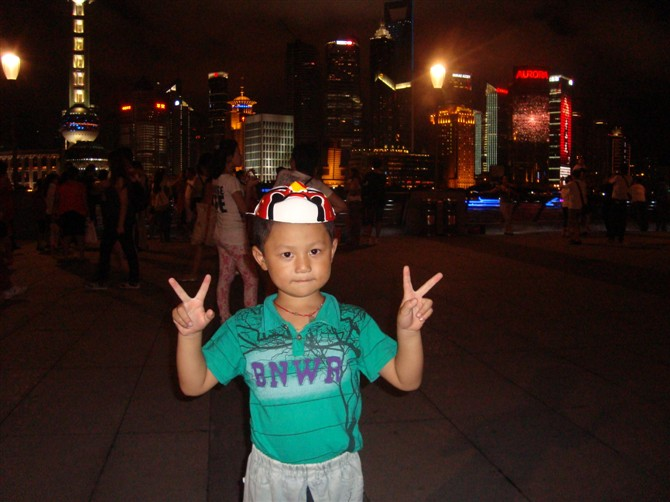
\includegraphics[width=\paperwidth]{Figure/30.jpg}
			};
			
			\node[anchor=center, text=DarkBlue] at ([yshift=-20cm]current page.north) {
				\begin{minipage}{0.85\paperwidth}
					\centering
					{\fontsize{36}{44}\sffamily\bfseries 强化学习} \\[0.5cm]
					{\fontsize{20}{28}\sffamily 从数学基础到机器人控制} \\[1.5cm]
					{\fontsize{14}{18}\kaishu 基于强化学习的机器人运动控制策略} \\[2cm]
					{\fontsize{16}{20}\Large 魏舟 } \\[0.5cm]
					{\large \today}
				\end{minipage}
			};
		\end{tikzpicture}
	\end{titlepage}
	
	\newpage
	\thispagestyle{empty}
	\vspace*{4cm}
	\begin{center}
		{\Large \kaishu 内容提要}
	\end{center}
	\vspace{1cm}
	
	本书从最基础的数学知识出发，系统介绍强化学习（Reinforcement Learning, RL）的理论、算法及其在机器人控制中的应用。全书共十二章：第1章回顾必要的数学基础；第2--4章建立马尔可夫决策过程的框架并介绍经典求解方法；第5--9章深入深度强化学习的核心算法；第10--12章聚焦机器人运动学、动力学及强化学习在实际机器人控制中的部署。
	
	本书的特点在于：（1）从概率论和线性代数的最基本概念开始，降低初学者的入门门槛；（2）所有算法均附有伪代码，便于读者实现；（3）在机器人控制部分，与Denavit-Hartenberg参数法和刚体动力学算法紧密衔接；（4）涵盖从仿真到真实机器人（Sim-to-Real）的最新研究进展。
	
	\vspace{2cm}
	\begin{flushright}
		\kaishu 魏舟 \\
		2025年7月
	\end{flushright}
	
	\newpage
	\tableofcontents
	
	\setcounter{page}{0}
	\thispagestyle{empty}
	\newpage
	
	% === CHAPTERS ===
	\chapter{数学基础}

\intro{``Mathematics is the language with which God has written the universe.''\par
\hfill --- Galileo Galilei\par
本章建立强化学习所需的数学基础。强化学习处于概率论、线性代数、优化理论和微积分的交叉点。掌握这些数学工具，是深入理解后续所有算法的前提。每一小节末尾均标注该知识点在强化学习中的具体应用场景，帮助读者建立概念之间的桥梁。}

% ======================================================================
\section{概率论基础}
% ======================================================================

概率论是强化学习的核心数学语言。智能体在不确定环境中决策，奖励信号带有随机性，状态转移可能是随机的--这些都要求我们使用概率工具来建模和分析。本节从随机变量的基本概念出发，逐步深入到重要性采样等高级技术。

% ----------------------------------------------------------------------
\subsection{随机变量与概率分布}
% ----------------------------------------------------------------------

\begin{mydefinition}{随机变量}
随机变量 $X$ 是从样本空间 $\Omega$ 到实数集 $\R$ 的一个可测函数。随机变量分为两类：
\begin{itemize}
    \item \textbf{离散随机变量}：取值于有限或可数无限集合$\{x_1, x_2, \dots\}$，由\textbf{概率质量函数}(PMF) $p(x) = \Pr(X = x)$ 描述。
    \item \textbf{连续随机变量}：取值于连续区间，由\textbf{概率密度函数}(PDF) $f(x)$ 描述，满足$\Pr(a \le X \le b) = \int_a^b f(x)\,dx$。
\end{itemize}
\end{mydefinition}

概率分布必须满足归一化条件：
\begin{myformula}
\sum_{x} p(x) = 1 \quad \text{(离散)}, \qquad \int_{-\infty}^{\infty} f(x)\,dx = 1 \quad \text{(连续)}
\end{myformula}

\textbf{常见的离散分布：}
\begin{itemize}
    \item \textbf{Bernoulli分布} $\mathrm{Bernoulli}(\theta)$：$p(x) = \theta^x (1-\theta)^{1-x}$，$x \in \{0,1\}$。描述单次二元试验。
    \item \textbf{分类分布 (Categorical)} $\mathrm{Cat}(\theta_1, \dots, \theta_K)$：$p(x = k) = \theta_k$，$\sum_k \theta_k = 1$。Bernoulli的多类推广。在RL中，随机策略 $\pi(a \mid s)$ 正是对每个状态$s$ 定义的一个分类分布。
    \item \textbf{二项分布} $\mathrm{Binomial}(n, \theta)$：$p(k) = \binom{n}{k} \theta^k (1-\theta)^{n-k}$。描述$n$ 次独立Bernoulli试验中成功的次数。
    \item \textbf{Poisson分布} $\mathrm{Poisson}(\lambda)$：$p(k) = \frac{\lambda^k e^{-\lambda}}{k!}$。描述单位时间内随机事件发生的次数，在排队论和强化学习的到达过程建模中有应用。
\end{itemize}

\textbf{常见的连续分布：}
\begin{itemize}
    \item \textbf{均匀分布} $U(a, b)$：$f(x) = \frac{1}{b-a}$，$x \in [a, b]$。
    \item \textbf{正态分布} $\mathcal{N}(\mu, \sigma^2)$：$f(x) = \frac{1}{\sqrt{2\pi\sigma^2}} \exp\left(-\frac{(x-\mu)^2}{2\sigma^2}\right)$。中心极限定理保证了许多随机现象的极限分布为正态分布。在RL中，策略梯度方法常用正态分布作为连续动作空间的策略参数化形式。
    \item \textbf{指数分布} $\mathrm{Exp}(\lambda)$：$f(x) = \lambda e^{-\lambda x}$，$x \ge 0$。具有无记忆性，与马尔可夫性质密切相关。
\end{itemize}

\begin{myTheorem}{概率分布函数的性质}
任一概率分布函数（PMF或PDF）$p(x)$ 满足：
\begin{enumerate}
    \item \textbf{非负性}：$p(x) \ge 0$ 对所有$x$ 成立。
    \item \textbf{归一化}：$\sum_x p(x) = 1$ 或$\int p(x)dx = 1$。
    \item \textbf{可加性}：对互斥事件 $A$ 和$B$，$\Pr(A \cup B) = \Pr(A) + \Pr(B)$。
\end{enumerate}
\end{myTheorem}

\begin{tikzpicture}[scale=1.2]
    \draw[->] (-0.5,0) -- (8,0) node[right] {$x$};
    \draw[->] (0,-0.2) -- (0,3.5) node[above] {$p(x)$};
    % Discrete PMF
    \foreach \x/\y in {1/1.2,2/2.8,3/2.0,4/0.8,5/0.3} {
        \draw[blue, thick] (\x,0) -- (\x,\y);
        \fill[blue] (\x,\y) circle (1.5pt);
        \fill[blue] (\x,0) circle (1.5pt);
    }
    \node[blue] at (3,-0.5) {离散分布 (PMF)};
    % Continuous PDF  
    \draw[domain=0.5:5.5,smooth,variable=\x,red,thick] plot ({\x+1.2},{2.0*exp(-(\x-2.5)^2/1.2)});
    \node[red] at (5.5,1.0) {连续分布 (PDF)};
\end{tikzpicture}

% ----------------------------------------------------------------------
\subsection{条件概率、贝叶斯公式与全概率公式}
% ----------------------------------------------------------------------

\begin{mydefinition}{条件概率}
事件 $A$ 在事代$B$ 已发生条件下的条件概率定义为：
\begin{myformula}
\Pr(A \mid B) = \frac{\Pr(A \cap B)}{\Pr(B)}, \quad \Pr(B) > 0
\end{myformula}
\end{mydefinition}

条件概率是强化学习的基石。策略$\pi(a \mid s)$ 本身就是条件概率：在状性$s$ 下选择动作 $a$ 的概率。状态转移概率$p(s' \mid s, a)$ 也是条件概率：在状性$s$ 执行动作 $a$ 后转移到 $s'$ 的概率。

由条件概率定义可直接导出\textbf{乘法法则}：
\begin{myformula}
\Pr(A \cap B) = \Pr(A \mid B) \Pr(B) = \Pr(B \mid A) \Pr(A)
\end{myformula}

推广分$n$ 个事件的\textbf{链式法则}：
\begin{myformula}
\Pr(A_1 \cap A_2 \cap \dots \cap A_n) = \Pr(A_1) \Pr(A_2 \mid A_1) \Pr(A_3 \mid A_1, A_2) \cdots \Pr(A_n \mid A_1, \dots, A_{n-1})
\end{myformula}

\textbf{链式法则在RL中的核心应用}：给定策略$\pi$ 和MDP，一条轨这$\tau = (s_0, a_0, s_1, a_1, \dots, s_T)$ 的概率为：
\begin{myformula}
\Pr(\tau) = p(s_0) \prod_{t=0}^{T-1} \pi(a_t \mid s_t) \, p(s_{t+1} \mid s_t, a_t)
\end{myformula}
这是策略梯度方法中似然比技巧的基础。

\begin{myTheorem}{全概率公式(Law of Total Probability)}
设$B_1, B_2, \dots, B_n$ 为样本空间的一个划分（互斥且穷尽），则对任意事件$A$：
\begin{myformula}
\Pr(A) = \sum_{i=1}^{n} \Pr(A \mid B_i) \Pr(B_i)
\end{myformula}
连续形式：$\Pr(A) = \int \Pr(A \mid B = b) \, f_B(b) \, db$。
\end{myTheorem}

\begin{proof}
由划分定义：$A = A \cap \left(\bigcup_{i=1}^{n} B_i\right) = \bigcup_{i=1}^{n} (A \cap B_i)$。由于$B_i$ 互斥，$(A \cap B_i)$ 也互斥，故：
\begin{align*}
\Pr(A) = \sum_{i=1}^{n} \Pr(A \cap B_i) = \sum_{i=1}^{n} \Pr(A \mid B_i) \Pr(B_i)
\end{align*}
\end{proof}

\textbf{全概率公式在RL中的应用}：Bellman方程的核心推导依赖全概率公式。状态值函数定义为：
\[
V^{\pi}(s) = \E_\pi[G_t \mid S_t = s] = \sum_a \pi(a \mid s) \sum_{s', r} p(s', r \mid s, a) [r + \gamma V^{\pi}(s')]
\]
这里对动使$a$ 求期望和对后继状性$(s', r)$ 求期望，本质上就是两次应用全概率公式。

\begin{myTheorem}{贝叶斯公式(Bayes' Rule)}
\begin{myformula}
\Pr(B_i \mid A) = \frac{\Pr(A \mid B_i) \Pr(B_i)}{\sum_{j=1}^{n} \Pr(A \mid B_j) \Pr(B_j)}
\end{myformula}
其中分母正是全概率公式。术语上：$\Pr(B_i)$ 为\textbf{先验概率}：$\Pr(B_i \mid A)$ 为\textbf{后验概率}：$\Pr(A \mid B_i)$ 为\textbf{似然}。
\end{myTheorem}

\begin{example}
\textbf{医学诊断与贝叶斯更新}：某疾病发病率为 $1\%$，检测准确率中$99\%$（真阳性率），假阳性率中$2\%$。若某人检测呈阳性，他真正患病的概率是多少？

计$D$ 为患病事件，$T^+$ 为检测阳性。已知：
\[
\Pr(D) = 0.01,\quad \Pr(T^+ \mid D) = 0.99,\quad \Pr(T^+ \mid \neg D) = 0.02
\]
由贝叶斯公式：
\begin{align*}
\Pr(D \mid T^+) &= \frac{0.99 \times 0.01}{0.99 \times 0.01 + 0.02 \times 0.99} \\
&= \frac{0.0099}{0.0099 + 0.0198} = \frac{0.0099}{0.0297} \approx 0.333
\end{align*}
代$33.3\%$！这个反直觉的结果说明：即使高准确率测试，对于罕见病，阳性结果也可能大部分是假阳性。

\textbf{RL启示}：在部分可观测环境中，智能体需要根据观测序列不断更新对隐藏状态的信念，这正是贝叶斯滤波的思想。
\end{example}

% ----------------------------------------------------------------------
\subsection{期望、方差与协方差}
% ----------------------------------------------------------------------

\begin{mydefinition}{期望 (Expectation)}
离散随机变量 $X$ 的期望为：
\[
\E[X] = \sum_{x} x \, p(x)
\]
连续随机变量：$\E[X] = \int x \, f(x) \, dx$。

对函数$g(X)$ 的期望：$\E[g(X)] = \sum_x g(x) p(x)$（离散）或$\int g(x) f(x) dx$（连续）。
\end{mydefinition}

\textbf{期望的线性性质}（极其重要）：
\begin{myformula}
\E[aX + bY] = a\E[X] + b\E[Y]
\end{myformula}
注意：线性性不要求 $X$ 和$Y$ 独立。这一性质简化了RL中大量推导。

\begin{mydefinition}{方差与标准差}
方差度量随机变量偏离其均值的程度：
\begin{align*}
\mathrm{Var}[X] &= \E[(X - \E[X])^2] = \E[X^2] - (\E[X])^2
\end{align*}
标准差$\sigma_X = \sqrt{\mathrm{Var}[X]}$，与 $X$ 具有相同量纲。
\end{mydefinition}

方差的性质：
\begin{itemize}
    \item $\mathrm{Var}[aX + b] = a^2 \mathrm{Var}[X]$
    \item 若$X, Y$ 独立，则 $\mathrm{Var}[X + Y] = \mathrm{Var}[X] + \mathrm{Var}[Y]$
    \item 若$X, Y$ 不独立，则$\mathrm{Var}[X + Y] = \mathrm{Var}[X] + \mathrm{Var}[Y] + 2\mathrm{Cov}[X, Y]$
\end{itemize}

\begin{mydefinition}{协方差与相关系数}
协方差度量两个随机变量的线性相关程度：
\[
\mathrm{Cov}[X, Y] = \E[(X - \E[X])(Y - \E[Y])] = \E[XY] - \E[X]\E[Y]
\]
相关系数（标准化协方差）：
\[
\rho_{XY} = \frac{\mathrm{Cov}[X, Y]}{\sqrt{\mathrm{Var}[X] \mathrm{Var}[Y]}} \in [-1, 1]
\]
\end{mydefinition}

\begin{remark} \textbf{为什么对RL重要？}
回报 $G_t = \sum_{k=0}^{\infty} \gamma^k R_{t+k+1}$ 是一个随机变量。RL算法的核心就是估计$\E[G_t \mid S_t = s]$（值函数）。方差在RL中同样关键：高方差意味着估计不稳定，actor-critic方法引入baseline的核心动机就是减少策略梯度估计的方差$\mathrm{Var}[\nabla_\theta J(\theta)]$。协方差在理解不同状态之间值估计的相关性、以及多任务强化学习中也很重要。
\end{remark}

% ----------------------------------------------------------------------
\subsection{大数定律与中心极限定理}
% ----------------------------------------------------------------------

\begin{myTheorem}{{大数定律（Law of Large Numbers, LLN）}}
设$X_1, X_2, \dots, X_n$ 为独立同分布 (i.i.d.) 随机变量，$\E[X_i] = \mu$。则样本均值依概率收敛于$\mu$：
\[
\bar{X}_n = \frac{1}{n} \sum_{i=1}^{n} X_i \xrightarrow{P} \mu \quad (n \to \infty)
\]
\emph{强}大数定律：$\bar{X}_n \xrightarrow{\text{a.s.}} \mu$（几乎必然收敛）。
\end{myTheorem}

LLN是统计估计方法的理论基础。在RL中，Monte Carlo方法的核心思想就是用大量采样轨迹的平均回报来估计值函数。例如，对状态$s$ 的$n$ 次访问得到的回报 $G^{(1)}, G^{(2)}, \dots, G^{(n)}$：
\[
V(s) \approx \frac{1}{n} \sum_{i=1}^{n} G^{(i)}
\]
LLN保证了当 $n \to \infty$ 时这个估计收敛到真实值。

\begin{myTheorem}{{中心极限定理（Central Limit Theorem, CLT）}}
设$X_1, \dots, X_n \overset{\text{i.i.d.}}{\sim} (\mu, \sigma^2)$，则标准化样本均值的分布收敛到标准正态分布：
\[
\frac{\bar{X}_n - \mu}{\sigma / \sqrt{n}} \xrightarrow{d} \mathcal{N}(0, 1) \quad (n \to \infty)
\]
等价地，$\bar{X}_n \approx \mathcal{N}\left(\mu, \frac{\sigma^2}{n}\right)$。
\end{myTheorem}

CLT告诉我们：估计误差大约以 $O(1/\sqrt{n})$ 的速率衰减，且误差近似服从正态分布。这为RL中构建置信区间和进行假设检验提供了理论基础。例如，在bandit问题中，Upper Confidence Bound (UCB) 算法正是基于Hoeffding不等式（CLT的泛化版本）来选择动作。

% ----------------------------------------------------------------------
\subsection{条件期望与全期望公式}
% ----------------------------------------------------------------------

\begin{mydefinition}{条件期望}
给定 $Y = y$ 时$X$ 的条件期望为：
\[
\E[X \mid Y = y] = \sum_x x \cdot \Pr(X = x \mid Y = y) \quad \text{或} \quad \int x \, f_{X \mid Y}(x \mid y) \, dx
\]
$\E[X \mid Y]$ 本身是一个关于$Y$ 的随机变量：当$Y = y$ 时取值为 $\E[X \mid Y = y]$。
\end{mydefinition}

\begin{myTheorem}{全期望公式(Law of Total Expectation)}
\begin{myformula}
\E[X] = \E_Y\big[\E_X[X \mid Y]\big]
\end{myformula}
即：无条件期望等于条件期望的期望。
\end{myTheorem}

\begin{proof}
对于离散情况：
\begin{align*}
\E_Y[\E_X[X \mid Y]] &= \sum_y \E[X \mid Y = y] \Pr(Y = y) \\
&= \sum_y \left(\sum_x x \Pr(X = x \mid Y = y)\right) \Pr(Y = y) \\
&= \sum_x x \sum_y \Pr(X = x, Y = y) = \sum_x x \Pr(X = x) = \E[X]
\end{align*}
\end{proof}

\textbf{全期望公式在RL中的核心应用}：它是Bellman方程推导的核心工具。例如，状态值函数$V^{\pi}(s) = \E[G_t \mid S_t = s]$：
\[
V^{\pi}(s) = \E[G_t \mid S_t = s] = \E[R_{t+1} + \gamma G_{t+1} \mid S_t = s]
\]
应用全期望公式，对$S_{t+1}$（和 $A_t$）取条件：
\begin{align*}
V^{\pi}(s) &= \E_{A_t \sim \pi(\cdot \mid s)}\left[\E_{S_{t+1}, R_{t+1}}\left[R_{t+1} + \gamma \E[G_{t+1} \mid S_{t+1}] \;\middle|\; S_t = s, A_t\right]\right] \\
&= \sum_a \pi(a \mid s) \sum_{s', r} p(s', r \mid s, a) \left[r + \gamma V^{\pi}(s')\right]
\end{align*}
这正是Bellman期望方程！可以说，理解全期望公式就理解了Bellman方程的本质。

全方差公式（方差分解）同样有用：
\[
\mathrm{Var}[X] = \E[\mathrm{Var}[X \mid Y]] + \mathrm{Var}[\E[X \mid Y]]
\]
在RL中，这一分解帮助我们理解回报方差中哪些来自环境随机性，哪些来自策略随机性。

% ----------------------------------------------------------------------
\subsection{重要性采样(Importance Sampling)}
% ----------------------------------------------------------------------

\begin{mydefinition}{重要性采样}
设我们希望估计$\E_{x \sim p}[f(x)]$，但难以代$p$ 采样。重要性采样利用一个易采样的提议分布$q$（满足$q(x) > 0$ 当$p(x) > 0$）：
\begin{myformula}
\E_{x \sim p}[f(x)] = \sum_x f(x) p(x) = \sum_x f(x) \frac{p(x)}{q(x)} q(x) = \E_{x \sim q}\left[\frac{p(x)}{q(x)} f(x)\right]
\end{myformula}
其中 $w(x) = p(x)/q(x)$ 称为\textbf{重要性权重}。
\end{mydefinition}

实际中，我们代$q$ 采样 $x^{(1)}, \dots, x^{(n)}$，构建估计：
\[
\hat{\mu}_{\mathrm{IS}} = \frac{1}{n} \sum_{i=1}^{n} w(x^{(i)}) f(x^{(i)})
\]

\textbf{在RL中的核心应用}：\textbf{离策略off-policy)学习}。当行为策略 $b$（用于采样）与目标策略$\pi$（待评估）不同时，我们需要用重要性采样校正分布差异。例如，在off-policy Monte Carlo中，一条轨这$\tau$ 的重要性权重为：
\[
w(\tau) = \prod_{t=0}^{T-1} \frac{\pi(A_t \mid S_t)}{b(A_t \mid S_t)}
\]
这本质上就是用重要性采样从$b$生成的轨迹中无偏估计$\pi$的值函数。

\begin{myTheorem}{重要性采样的无偏性与方差}
$\E_q[w(x) f(x)] = \E_p[f(x)]$，故IS估计是无偏的。其方差为：
\[
\mathrm{Var}_q[w(x) f(x)] = \E_q[w(x)^2 f(x)^2] - (\E_p[f(x)])^2
\]
当$p$ 和$q$ 差异很大时，重要性权重方差极大，导致估计不可靠。这就解释了为什么off-policy方法在策略差异大时需要额外的方差削减技术。
\end{myTheorem}

\textbf{加权重要性采样(Weighted IS)} 是一种偏差方差权衡：
\[
\hat{\mu}_{\mathrm{WIS}} = \frac{\sum_{i=1}^{n} w(x^{(i)}) f(x^{(i)})}{\sum_{i=1}^{n} w(x^{(i)})}
\]
WIS是有偏的，但方差通常远小于普通IS。在RL中，加权重要性采样常用于off-policy策略评估。

\begin{example}
设目标分布$p = \mathcal{N}(0, 1)$（标准正态），我们希望估计$\E_p[x^2] = 1$（方差）。
若我们只能用 $q = \mathcal{N}(1, 1)$ 采样。重要性权重：
\begin{align*}
w(x) = \frac{\frac{1}{\sqrt{2\pi}} e^{-x^2/2}}{\frac{1}{\sqrt{2\pi}} e^{-(x-1)^2/2}} = \exp\left(-\frac{x^2}{2} + \frac{(x-1)^2}{2}\right) = \exp\left(\frac{1}{2} - x\right)
\end{align*}
从$q$ 中采$n=10000$ 个样本并计算IS估计，可得到接近$1.0$的估计值（尽管$q$与$p$有偏移）。普通IS的权重方差较大，但WIS能给出更稳定的估计。
\end{example}

% ======================================================================
\section{线性代数基础}
% ======================================================================

强化学习中，值函数是向量（每个状态对应一个分量），转移概率是矩阵，策略评估本质上是求解线性方程组。扎实的线性代数是理解算法收敛性和实现高效计算的关键。

% ----------------------------------------------------------------------
\subsection{向量与矩阵}
% ----------------------------------------------------------------------

\begin{mydefinition}{向量}
$n$ 维实向量 $\mathbf{x} \in \R^n$ 是一个有序的 $n$ 元组：$\mathbf{x} = (x_1, x_2, \dots, x_n)\T$。在RL中，值函数$\mathbf{V} \in \R^{|\states|}$ 是一个向量，每一分量对应一个状态的值。
\end{mydefinition}

\textbf{向量运算：}
\begin{itemize}
    \item \textbf{内积}：$\langle \mathbf{x}, \mathbf{y} \rangle = \mathbf{x}\T \mathbf{y} = \sum_{i=1}^{n} x_i y_i$
    \item \textbf{外积}：$\mathbf{x} \mathbf{y}\T \in \R^{n \times m}$（若 $\mathbf{x} \in \R^n, \mathbf{y} \in \R^m$：
    \item \textbf{线性组合}：$\sum_{i=1}^{k} c_i \mathbf{v}_i$
\end{itemize}

在RL中，值函数的Bellman方程可以紧凑表示为向量形式：
\[
\mathbf{V}^{\pi} = \mathbf{R}^{\pi} + \gamma \mathbf{P}^{\pi} \mathbf{V}^{\pi}
\]
其中 $\mathbf{P}^{\pi} \in \R^{|\states| \times |\states|}$ 是策略$\pi$下的状态转移矩阵。

\begin{mydefinition}{矩阵}
$m \times n$ 矩阵 $\mathbf{A} \in \R^{m \times n}$：
\[
\mathbf{A} = \begin{bmatrix}
a_{11} & a_{12} & \cdots & a_{1n} \\
a_{21} & a_{22} & \cdots & a_{2n} \\
\vdots & \vdots & \ddots & \vdots \\
a_{m1} & a_{m2} & \cdots & a_{mn}
\end{bmatrix}
\]
\end{mydefinition}

\textbf{矩阵乘法} $(\mathbf{AB})_{ij} = \sum_{k} a_{ik} b_{kj}$：$\mathbf{A} \in \R^{m \times k}$：$\mathbf{B} \in \R^{k \times n}$）。矩阵乘法不满足交换律：$\mathbf{AB} \neq \mathbf{BA}$（一般情况）。

\textbf{特殊矩阵：}
\begin{itemize}
    \item \textbf{单位矩阵} $\mathbf{I}_n$，$(\mathbf{I})_{ij} = \delta_{ij}$（Kronecker delta），$\mathbf{I}\mathbf{A} = \mathbf{A}\mathbf{I} = \mathbf{A}$
    \item \textbf{对角矩阵} $\mathrm{diag}(d_1, \dots, d_n)$：非对角线元素为集
    \item \textbf{随机矩阵}：每行元素非负且和为1。\textbf{MDP的转移矩阵$\mathbf{P}^{\pi}$ 正是一个随机矩阵}。
\end{itemize}

% ----------------------------------------------------------------------
\subsection{特征值与特征向量}
% ----------------------------------------------------------------------

\begin{mydefinition}{特征值与特征向量}
对方阵$\mathbf{A} \in \R^{n \times n}$，若存在非零向量 $\mathbf{v}$ 和标量$\lambda$ 满足：
\begin{myformula}
\mathbf{A} \mathbf{v} = \lambda \mathbf{v}
\end{myformula}
分$\lambda$ 中$\mathbf{A}$ 的\textbf{特征值}：$\mathbf{v}$ 为对应的\textbf{特征向量}。
\end{mydefinition}

特征值由特征方程 $\det(\mathbf{A} - \lambda \mathbf{I}) = 0$ 确定。$n$ 阶矩阵有 $n$ 个特征值（计重数）。

\begin{myTheorem}{谱半征(Spectral Radius)}
矩阵 $\mathbf{A}$ 的谱半径定义为：
\[
\rho(\mathbf{A}) = \max_{i} |\lambda_i|
\]
其中 $\lambda_i$ 遍历 $\mathbf{A}$ 的所有特征值。

\textbf{核心结论}：对于随机矩阵$\mathbf{P}$（如MDP的转移矩阵）：$\rho(\mathbf{P}) = 1$。进一步，$\rho(\gamma \mathbf{P}^{\pi}) = \gamma < 1$（当 $\gamma < 1$）。这正是Bellman算子为压缩映射的代数本质。
\end{myTheorem}

\begin{myTheorem}{特征分解 (Eigendecomposition)}
若$\mathbf{A} \in \R^{n \times n}$ 机$n$ 个线性无关的特征向量 $\mathbf{v}_1, \dots, \mathbf{v}_n$（对应特征值$\lambda_1, \dots, \lambda_n$），则：
\[
\mathbf{A} = \mathbf{V} \boldsymbol{\Lambda} \mathbf{V}^{-1}
\]
其中 $\mathbf{V} = [\mathbf{v}_1 \; \cdots \; \mathbf{v}_n]$：$\boldsymbol{\Lambda} = \mathrm{diag}(\lambda_1, \dots, \lambda_n)$。
\end{myTheorem}

\textbf{特征分解在RL中的应用}：通过特征分解，Bellman方程的解析解 $\mathbf{V}^{\pi} = (\mathbf{I} - \gamma \mathbf{P}^{\pi})^{-1} \mathbf{R}^{\pi}$ 可写为：
\[
\mathbf{V}^{\pi} = \sum_{k=0}^{\infty} \gamma^k (\mathbf{P}^{\pi})^k \mathbf{R}^{\pi}
\]
使用特征分解 $(\mathbf{P}^{\pi})^k = \mathbf{V} \boldsymbol{\Lambda}^k \mathbf{V}^{-1}$，可见当 $\gamma < 1$ 时$\gamma^k \boldsymbol{\Lambda}^k \to \mathbf{0}$，保证了解的存在唯一性。

% ----------------------------------------------------------------------
\subsection{矩阵逆与伪逆}
% ----------------------------------------------------------------------

\begin{mydefinition}{逆矩阵}
若存在方阵$\mathbf{A}^{-1}$ 满足 $\mathbf{A} \mathbf{A}^{-1} = \mathbf{A}^{-1} \mathbf{A} = \mathbf{I}$，则称$\mathbf{A}$ 为\textbf{可逆}（非奇异）。
\end{mydefinition}

可逆的充要条件：$\det(\mathbf{A}) \neq 0$，等价于所有特征值均非零。

\textbf{在RL中的应用}：Bellman方程的解析解 $\mathbf{V}^{\pi} = (\mathbf{I} - \gamma \mathbf{P}^{\pi})^{-1} \mathbf{R}^{\pi}$ 需要求 $(\mathbf{I} - \gamma \mathbf{P}^{\pi})$ 的逆。当 $\gamma < 1$ 时，该矩阵总是可逆的，因为$\rho(\gamma \mathbf{P}^{\pi}) = \gamma < 1$，所以$\mathbf{I} - \gamma \mathbf{P}^{\pi}$ 的所有特征值满足$1 - \gamma \lambda_i > 0$，非奇异。

\textbf{Neumann级数}给出了逆的一个有用的级数表示：
\begin{myformula}
(\mathbf{I} - \mathbf{A})^{-1} = \sum_{k=0}^{\infty} \mathbf{A}^k, \quad \text{当} \rho(\mathbf{A}) < 1
\end{myformula}
代$\mathbf{A} = \gamma \mathbf{P}^{\pi}$：$\rho(\gamma \mathbf{P}^{\pi}) = \gamma < 1$），得：
\[
\mathbf{V}^{\pi} = \sum_{k=0}^{\infty} \gamma^k (\mathbf{P}^{\pi})^k \mathbf{R}^{\pi}
\]
这正是回报定习$\mathbf{V}^{\pi} = \E[\sum_{k=0}^{\infty} \gamma^k \mathbf{R}_{t+k+1}^{\pi}]$ 的矩阵形式。

\begin{mydefinition}{Moore-Penrose伪逆}
对任意矩阵$\mathbf{A} \in \R^{m \times n}$（可以不是方阵），伪逆$\mathbf{A}^{+} \in \R^{n \times m}$ 满足四条Penrose条件：
\begin{itemize}
    \item $\mathbf{A} \mathbf{A}^{+} \mathbf{A} = \mathbf{A}$
    \item $\mathbf{A}^{+} \mathbf{A} \mathbf{A}^{+} = \mathbf{A}^{+}$
    \item $(\mathbf{A} \mathbf{A}^{+})\T = \mathbf{A} \mathbf{A}^{+}$
    \item $(\mathbf{A}^{+} \mathbf{A})\T = \mathbf{A}^{+} \mathbf{A}$
\end{itemize}
\end{mydefinition}

伪逆在RL的最小二乘方法中有重要应用。LSTD (Least-Squares Temporal Difference) 和LSPI (Least-Squares Policy Iteration) 都需要求解超定线性系统，使用伪逆给出最小范数最小二乘解。

% ----------------------------------------------------------------------
\subsection{线性方程组的求解}
% ----------------------------------------------------------------------

考虑线性方程组 $\mathbf{A} \mathbf{x} = \mathbf{b}$，其中$\mathbf{A} \in \R^{n \times n}$：$\mathbf{b} \in \R^n$。

\begin{itemize}
    \item \textbf{直接法}：若 $\mathbf{A}$ 可逆，解为 $\mathbf{x} = \mathbf{A}^{-1} \mathbf{b}$。计算复杂度 $O(n^3)$（高斯消元）。适用于小规模问题（如小型GridWorld）。
    \item \textbf{迭代法}：对大规模问题（如$|\states| > 10^6$），直接求逆不可行，需要迭代求解。这正是动态规划方法（策略迭代、值迭代）在做的。
\end{itemize}

\textbf{迭代法的基本框架}：将 $\mathbf{A}$ 分裂中$\mathbf{A} = \mathbf{M} - \mathbf{N}$：$\mathbf{M}$ 易求逆），则迭代格式为：
\[
\mathbf{x}^{(k+1)} = \mathbf{M}^{-1} \mathbf{N} \mathbf{x}^{(k)} + \mathbf{M}^{-1} \mathbf{b}
\]

\textbf{在RL中}：Bellman方程 $\mathbf{V} = \mathbf{R}^{\pi} + \gamma \mathbf{P}^{\pi} \mathbf{V}$ 可写为标准形式$(\mathbf{I} - \gamma \mathbf{P}^{\pi}) \mathbf{V} = \mathbf{R}^{\pi}$。策略评估的迭代格式 $\mathbf{V}^{(k+1)} = \mathbf{R}^{\pi} + \gamma \mathbf{P}^{\pi} \mathbf{V}^{(k)}$ 正是可$\mathbf{M} = \mathbf{I}$：$\mathbf{N} = \gamma \mathbf{P}^{\pi}$ 的迭代法（Richardson迭代）。

迭代法的收敛速率用$\rho(\mathbf{M}^{-1} \mathbf{N})$ 决定。对上述迭代，收敛速率中$\rho(\gamma \mathbf{P}^{\pi}) = \gamma$：$\gamma$ 越接这，收敛越快。

% ----------------------------------------------------------------------
\subsection{向量与矩阵范数}
% ----------------------------------------------------------------------

\begin{mydefinition}{向量范数}
向量 $\mathbf{x} \in \R^n$ 的$L_p$ 范数定义为：
\begin{align*}
L_0\text{（伪）范数：}&\quad \|\mathbf{x}\|_0 = \text{非零元素个数} \\
L_1\text{范数：}&\quad \|\mathbf{x}\|_1 = \sum_{i=1}^{n} |x_i| \\
L_2\text{范数（欧氏范数）：}&\quad \|\mathbf{x}\|_2 = \sqrt{\sum_{i=1}^{n} x_i^2} \\
L_\infty\text{范数（最大范数）：}&\quad \|\mathbf{x}\|_\infty = \max_{i} |x_i|
\end{align*}
\end{mydefinition}

\textbf{在RL中的使用}：
\begin{itemize}
    \item \textbf{$L_\infty$范数}用于DP收敛准则：$\|\mathbf{V}^{(k+1)} - \mathbf{V}^{(k)}\|_\infty < \theta$ 意味着每个状态的值估计变化都不超过$\theta$，是策略评估停止条件的自然选择。
    \item \textbf{$L_2$范数}用于最小二乘方法：LSTD、DQN中的TD目标本质上是Minimizing Bellman residual的$L_2$范数。
    \item \textbf{$L_1$范数}用于稀疏性约束：LASSO正则化可获得稀疏值函数表示，在特征选择和可解释RL中有应用。
\end{itemize}

\begin{mydefinition}{诱导矩阵范数}
由向量范数诱导的矩阵范数：
\[
\|\mathbf{A}\|_p = \sup_{\mathbf{x} \neq \mathbf{0}} \frac{\|\mathbf{A}\mathbf{x}\|_p}{\|\mathbf{x}\|_p}
\]
常用诱导范数：
\begin{itemize}
    \item $\|\mathbf{A}\|_1 = \max_j \sum_i |a_{ij}|$（最大列和）
    \item $\|\mathbf{A}\|_\infty = \max_i \sum_j |a_{ij}|$（最大行和）
    \item $\|\mathbf{A}\|_2 = \sqrt{\rho(\mathbf{A}\T \mathbf{A})}$（谱范数：
\end{itemize}
\end{mydefinition}

\textbf{关键性质}：对任意诱导矩阵范数：$\rho(\mathbf{A}) \le \|\mathbf{A}\|$。对随机矩阵 $\mathbf{P}$：$\|\mathbf{P}\|_\infty = 1$（因为每行和中）。

% ----------------------------------------------------------------------
\subsection{梯度与Hessian矩阵}
% ----------------------------------------------------------------------

\begin{mydefinition}{梯度}
多元函数 $f: \R^n \to \R$ 在点 $\mathbf{x}$ 的梯度是偏导数构成的列向量：
\begin{myformula}
\nabla f(\mathbf{x}) = \left(\frac{\partial f}{\partial x_1}, \frac{\partial f}{\partial x_2}, \dots, \frac{\partial f}{\partial x_n}\right)\T
\end{myformula}
梯度指向函数增长最快的方向，$-\nabla f(\mathbf{x})$ 指向最速下降方向。
\end{mydefinition}

\textbf{关键梯度计算}（在RL中极其常用）：
\begin{itemize}
    \item $\nabla_{\mathbf{x}} (\mathbf{a}\T \mathbf{x}) = \mathbf{a}$
    \item $\nabla_{\mathbf{x}} (\mathbf{x}\T \mathbf{A} \mathbf{x}) = (\mathbf{A} + \mathbf{A}\T) \mathbf{x}$（若 $\mathbf{A}$ 对称则为 $2\mathbf{A}\mathbf{x}$：
    \item $\nabla_{\mathbf{x}} \|\mathbf{x}\|_2^2 = 2\mathbf{x}$
\end{itemize}

\begin{mydefinition}{Jacobian矩阵}
向量值函数$\mathbf{f}: \R^n \to \R^m$ 的Jacobian矩阵 $\mathbf{J} \in \R^{m \times n}$：
\[
(\mathbf{J})_{ij} = \frac{\partial f_i}{\partial x_j}
\]

\textbf{Hessian矩阵}是梯度函数的Jacobian（对标量函数 $f$）：
\[
\mathbf{H}_f(\mathbf{x}) = \nabla^2 f(\mathbf{x}) = \begin{bmatrix}
\frac{\partial^2 f}{\partial x_1^2} & \cdots & \frac{\partial^2 f}{\partial x_1 \partial x_n} \\
\vdots & \ddots & \vdots \\
\frac{\partial^2 f}{\partial x_n \partial x_1} & \cdots & \frac{\partial^2 f}{\partial x_n^2}
\end{bmatrix}_{n \times n}
\]
\end{mydefinition}

Hessian矩阵总是对称的（若$f$二阶连续可导）。Hessian刻画了函数的曲率：
\begin{itemize}
    \item $\mathbf{H} \succ 0$（正定），$f$ 在该点局部严格凸
    \item $\mathbf{H} \prec 0$（负定），$f$ 在该点局部严格凹
    \item $\mathbf{H}$ 不定：鞍点
\end{itemize}

\begin{remark} \textbf{RL中的应用}：
\begin{itemize}
    \item \textbf{策略梯度}：$\nabla_\theta J(\theta) = \E_\tau[\sum_t \nabla_\theta \log \pi_\theta(a_t \mid s_t) \cdot G_t]$，核心是计算对数策略的梯度。
    \item \textbf{自然梯度}：使用Fisher信息矩阵（对数似然的Hessian的负期望）进行参数更新，$\theta \leftarrow \theta + \alpha \mathbf{F}^{-1} \nabla_\theta J(\theta)$，实现了参数空间中的``不变''更新。
    \item \textbf{TRPO/PPO}：使用KL散度的Hessian（即Fisher矩阵）约束策略更新幅度。
    \item \textbf{二阶优化}：Newton法$\theta \leftarrow \theta - \mathbf{H}^{-1} \nabla f(\theta)$，收敛更快但每次迭代代价大。
\end{itemize}
\end{remark}

% ======================================================================
\section{优化基础}
% ======================================================================

优化是强化学习的另一支柱。值函数的最优性由Bellman最优方程刻画，本质是一个不动点问题；策略的改进等价于对策略空间的最优化；策略梯度方法直接对期望回报进行梯度上升。理解优化理论有助于深刻把握RL算法设计的内在逻辑。

% ----------------------------------------------------------------------
\subsection{凸集与凸函数}
% ----------------------------------------------------------------------

\begin{mydefinition}{凸集}
集合 $C \subseteq \R^n$ 称为凸集，若对任意$\mathbf{x}, \mathbf{y} \in C$ 和任意$\lambda \in [0, 1]$，有：
\[
\lambda \mathbf{x} + (1 - \lambda) \mathbf{y} \in C
\]
即：连接集合内任意两点的线段完全包含在集合中。
\end{mydefinition}

\begin{mydefinition}{凸函数}
定义在凸集$C$ 上的函数 $f$ 称为凸函数，若对任意 $\mathbf{x}, \mathbf{y} \in C$ 和$\lambda \in [0, 1]$：
\[
f(\lambda \mathbf{x} + (1 - \lambda) \mathbf{y}) \le \lambda f(\mathbf{x}) + (1 - \lambda) f(\mathbf{y})
\]
严格凸：不等式严格成立（$\mathbf{x} \neq \mathbf{y}$，$\lambda \in (0,1)$）。若不等式反向，则为\textbf{凹函数}。
\end{mydefinition}

\begin{tikzpicture}[scale=1.0]
    % Convex function
    \draw[->] (-0.5,0) -- (4,0) node[right] {$x$};
    \draw[->] (0,-0.5) -- (0,3.5) node[above] {$f(x)$};
    \draw[domain=0.2:3.8,smooth,variable=\x,blue,thick] plot ({\x},{0.3*(\x-2)^2+0.8});
    \draw[red,dashed] (0.8,{0.3*(0.8-2)^2+0.8}) -- (3.2,{0.3*(3.2-2)^2+0.8});
    \fill[red] (0.8,{0.3*(0.8-2)^2+0.8}) circle (1.5pt);
    \fill[red] (3.2,{0.3*(3.2-2)^2+0.8}) circle (1.5pt);
    \node at (2,-0.8) {凸函数：弦在函数上方};
\end{tikzpicture}
\qquad
\begin{tikzpicture}[scale=1.0]
    % Non-convex function  
    \draw[->] (-0.5,0) -- (4,0) node[right] {$x$};
    \draw[->] (0,-1.5) -- (0,2.0) node[above] {$f(x)$};
    \draw[domain=0.2:3.8,smooth,variable=\x,red,thick] plot ({\x},{1.5*sin(1.8*\x r)});
    \node at (2,-2.0) {非凸函数：存在局部最优};
\end{tikzpicture}

\textbf{凸函数的关键性质：}
\begin{enumerate}
    \item \textbf{局部最小值即全局最小值}：凸函数的任何局部极小点必为全局最小点。这是凸优化问题``容易''的根本原因。
    \item \textbf{一阶条件}：若 $f$ 可微，则 $f$ 函$\iff$ $f(\mathbf{y}) \ge f(\mathbf{x}) + \nabla f(\mathbf{x})\T (\mathbf{y} - \mathbf{x})$ 对所机$\mathbf{x}, \mathbf{y}$ 成立（函数图像在切线上方）。
    \item \textbf{二阶条件}：若 $f$ 二阶可微，则 $f$ 函$\iff$ $\nabla^2 f(\mathbf{x}) \succeq 0$（Hessian半正定）对所机$\mathbf{x}$ 成立。
\end{enumerate}

\begin{remark} \textbf{RL中的凸性}，
值函数的Bellman算子不是凸的（因为是线性算子），但许多RL子问题具有凸结构：
\begin{itemize}
    \item \textbf{线性函数逼近下的策略评估}：目标函数$\|\mathbf{V}_\theta - (\mathbf{R} + \gamma \mathbf{P} \mathbf{V}_\theta)\|^2$ 关于线性参数$\theta$是凸的（实际上是一个线性最小二乘问题）。
    \item \textbf{值迭代}：Bellman最优算子$\mathcal{T} V(s) = \max_a [R(s,a) + \gamma \sum_{s'} P(s' \mid s,a) V(s')]$ 关于 $V$ 是单调的但不是凸的（因$\max$）。
    \item \textbf{策略梯度}：目样$J(\theta)$ 通常是非凸的，这就是为什么策略梯度方法只能收敛到局部最优。
\end{itemize}
\end{remark}

% ----------------------------------------------------------------------
\subsection{梯度下降法}
% ----------------------------------------------------------------------

\begin{mydefinition}{梯度下降 (Gradient Descent)}
对于无约束优化问题$\min_{\mathbf{x} \in \R^n} f(\mathbf{x})$，梯度下降迭代：
\begin{myformula}
\mathbf{x}_{k+1} = \mathbf{x}_k - \alpha_k \nabla f(\mathbf{x}_k)
\end{myformula}
其中 $\alpha_k > 0$ 为\textbf{步长}（学习率）。
\end{mydefinition}

\begin{tikzpicture}[scale=1.1]
    % Contour plot of a quadratic
    \draw[->] (-0.5,0) -- (5,0) node[right] {$x_1$};
    \draw[->] (0,-0.5) -- (0,4) node[above] {$x_2$};
    \draw[blue!40,thick] (2.5,2.5) ellipse (1.8 and 1.5);
    \draw[blue!40,thick] (2.5,2.5) ellipse (1.2 and 1.0);
    \draw[blue!40,thick] (2.5,2.5) ellipse (0.6 and 0.5);
    \draw[blue!40,thick] (2.5,2.5) ellipse (0.2 and 0.15);
    \fill[red] (2.5,2.5) circle (2pt) node[below right] {$\mathbf{x}^*$};
    % Gradient descent path
    \fill (1.5,1.0) circle (1.5pt);
    \draw[->,red,thick] (1.5,1.0) -- (2.0,1.5);
    \draw[->,red,thick] (2.0,1.5) -- (2.25,1.9);
    \draw[->,red,thick] (2.25,1.9) -- (2.4,2.2);
    \draw[->,red,thick] (2.4,2.2) -- (2.47,2.38);
    \node at (1.5,0.5) {梯度下降轨迹};
\end{tikzpicture}

\textbf{步长选择}至关重要：
\begin{itemize}
    \item $\alpha$ 太小：收敛缓慢，浪费计算资源
    \item $\alpha$ 太大：可能震荡甚至发数
    \item \textbf{精确线搜索}：$\alpha_k = \arg\min_{\alpha > 0} f(\mathbf{x}_k - \alpha \nabla f(\mathbf{x}_k))$
    \item \textbf{Armijo条件}：$\alpha_k$ 满足 $f(\mathbf{x}_k - \alpha \nabla f(\mathbf{x}_k)) \le f(\mathbf{x}_k) - c\alpha \|\nabla f(\mathbf{x}_k)\|^2$，$c \in (0, 1)$
    \item \textbf{学习率衰减}：$\alpha_k = \frac{\alpha_0}{1 + \text{decay} \cdot k}$，常用于SGD的RL应用
\end{itemize}

\begin{myTheorem}{梯度下降的收敛性（$L$-光滑函数）}
计$f$ 是$L$-光滑函数：$\nabla f$ 是$L$-Lipschitz连续：$\|\nabla f(\mathbf{x}) - \nabla f(\mathbf{y})\| \le L \|\mathbf{x} - \mathbf{y}\|$）且有下界。若取常数步长$\alpha \le 1/L$，则梯度下降满足：
\[
\min_{0 \le k < K} \|\nabla f(\mathbf{x}_k)\|^2 \le \frac{2L(f(\mathbf{x}_0) - f^*)}{K}
\]
即收敛速率中$O(1/K)$。若 $f$ 进一步是 $\mu$-强凸的，则线性收敛：$f(\mathbf{x}_k) - f^* \le (1 - \mu/L)^k (f(\mathbf{x}_0) - f^*)$。
\end{myTheorem}

\begin{remark} \textbf{梯度下降与RL中的策略迭代}，
策略迭代的改进步骤本质上是广义的梯度下降：在策略空间中，沿值函数增长的方向更新策略。而值迭代中Bellman最优算子的不动点迭代可以看作求解隐式最优性方程的一种``最速下降'方法。自然策略梯度则使用Fisher信息矩阵作为预处理器，实现了参数空间中的不变梯度下降。
\end{remark}

% ----------------------------------------------------------------------
\subsection{随机梯度下降 (SGD)}
% ----------------------------------------------------------------------

在实际RL中，我们通常不知道完整的目标函数，而是通过采样获得梯度的随机估计。

\begin{mydefinition}{随机梯度下降}
目标 $\min_\theta F(\theta) = \E_{z \sim D}[f(\theta; z)]$。SGD迭代：
\begin{myformula}
\theta_{k+1} = \theta_k - \alpha_k \hat{\nabla} f(\theta_k; z_k)
\end{myformula}
其中 $z_k$ 是从数据分布 $D$ 中采样的一个（或一批）随机样本：$\hat{\nabla}$ 是无偏梯度估计：$\E_{z}[\hat{\nabla} f(\theta; z)] = \nabla F(\theta)$。
\end{mydefinition}

SGD的收敛分析需要额外的条件。经典结果（Robbins-Monro）要求步长满足：
\[
\sum_{k=1}^{\infty} \alpha_k = \infty, \qquad \sum_{k=1}^{\infty} \alpha_k^2 < \infty
\]
典型选择：$\alpha_k = \frac{1}{k}$ 我$\alpha_k = \frac{c}{\sqrt{k}}$。

\textbf{SGD在RL中的普遍性}：几乎所有的现代深度RL方法都使用SGD或其变体（Adam、RMSprop等）。原因很简单：环境模型未知，我们只能通过与环境的交互获得有限的样本数据来估计梯度。例如：
\begin{itemize}
    \item \textbf{DQN}：用经验回放（replay buffer）采样z = (s, a, r, s')$，对Q网络的参数\theta$执行SGD来最小化TD误差。
    \item \textbf{策略梯度}：$\nabla_\theta J \approx \frac{1}{N} \sum_{i=1}^{N} \sum_{t=0}^{T} \nabla_\theta \log \pi_\theta(a_t^{(i)} \mid s_t^{(i)}) \cdot \hat{G}_t^{(i)}$，用一批轨迹估计梯度。
    \item \textbf{Actor-Critic}：Actor用SGD更新策略参数，Critic用SGD更新值函数参数。
\end{itemize}

% ----------------------------------------------------------------------
\subsection{约束优化与Lagrange乘子法}
% ----------------------------------------------------------------------

\begin{mydefinition}{Lagrange乘子法}
考虑等式约束优化问题：
\[
\min_{\mathbf{x}} f(\mathbf{x}), \quad \text{s.t. } g_i(\mathbf{x}) = 0 \; (i = 1, \dots, m)
\]
定义Lagrange函数 $\mathcal{L}(\mathbf{x}, \boldsymbol{\lambda}) = f(\mathbf{x}) + \sum_{i=1}^{m} \lambda_i g_i(\mathbf{x})$。必要条件（KKT）：
\[
\nabla_{\mathbf{x}} \mathcal{L} = \nabla f(\mathbf{x}) + \sum_{i=1}^{m} \lambda_i \nabla g_i(\mathbf{x}) = \mathbf{0}, \quad g_i(\mathbf{x}) = 0
\]
\end{mydefinition}

对于不等式约条$h_j(\mathbf{x}) \le 0$，引入非负Lagrange乘子 $\mu_j \ge 0$，KKT条件补充互补松弛条件：$\mu_j h_j(\mathbf{x}) = 0$。

\textbf{对偶性(Duality)}：Lagrange对偶函数：
\[
q(\boldsymbol{\lambda}, \boldsymbol{\mu}) = \inf_{\mathbf{x}} \mathcal{L}(\mathbf{x}, \boldsymbol{\lambda}, \boldsymbol{\mu})
\]
对偶问题是$\max_{\boldsymbol{\lambda}, \boldsymbol{\mu} \ge 0} q(\boldsymbol{\lambda}, \boldsymbol{\mu})$。弱对偶性保证对偶最优值$\le$ 原始最优值；强对偶性（Slater条件成立时）保证等号成立。

\begin{remark} \textbf{Lagrange乘子法在高级RL中的关键应用}：
\begin{itemize}
    \item \textbf{TRPO}：$\max_\theta \E[\pi_\theta] \; \text{s.t.} \; D_{\mathrm{KL}}(\pi_{\mathrm{old}} \| \pi_\theta) \le \delta$。约束优化确保策略更新不过大，使用Lagrange乘子或对偶梯度下降处理。
    \item \textbf{PPO}：用截断（clipping）机制替代显式KL约束，等价于一种``转'约束优化。
    \item \textbf{约束马尔可夫决策过程 (CMDP)}：在安全RL中，额外约束期望代价不超过阈值。Lagrangian方法将约束问题转化为无约束max-min问题。
    \item \textbf{最大熵RL (SAC)}：目样$J(\pi) = \sum_t \E[r_t + \alpha \mathcal{H}(\pi(\cdot \mid s_t))]$：$\alpha$ 通过Lagrangian方法自适应调整以满足目标熵约束。
\end{itemize}
\end{remark}

% ----------------------------------------------------------------------
\subsection{KL散度}
% ----------------------------------------------------------------------

\begin{mydefinition}{KL散度 (Kullback-Leibler Divergence)}
对离散分布$p$ 和$q$（满足$q(x) = 0 \Rightarrow p(x) = 0$）：
\begin{myformula}
D_{\mathrm{KL}}(p \| q) = \sum_{x} p(x) \log \frac{p(x)}{q(x)}
\end{myformula}
对连续分布：$D_{\mathrm{KL}}(p \| q) = \int p(x) \log \frac{p(x)}{q(x)} dx$。
\end{mydefinition}

\textbf{KL散度的性质：}
\begin{itemize}
    \item \textbf{非负性}：$D_{\mathrm{KL}}(p \| q) \ge 0$，等号当且仅当$p = q$（几乎处处）。由Gibbs不等式可证。
    \item \textbf{非对称性}：$D_{\mathrm{KL}}(p \| q) \neq D_{\mathrm{KL}}(q \| p)$（一般情况）。这不是一个真正的距离度量。
    \item \textbf{与交叉熵的关系}：$D_{\mathrm{KL}}(p \| q) = H(p, q) - H(p)$，其中$H(p, q) = -\sum_x p(x) \log q(x)$ 是交叉熵，$H(p) = -\sum_x p(x) \log p(x)$ 是熵。
\end{itemize}

\begin{example}
\textbf{KL散度计算示例}：设 $p = \mathrm{Bernoulli}(0.7)$，$q = \mathrm{Bernoulli}(0.3)$。
\begin{align*}
D_{\mathrm{KL}}(p \| q) &= 0.7 \log \frac{0.7}{0.3} + 0.3 \log \frac{0.3}{0.7} \\
&= 0.7 \times 0.8473 + 0.3 \times (-0.8473) \\
&= 0.5931 - 0.2542 = 0.3389
\end{align*}
反过来$D_{\mathrm{KL}}(q \| p) = 0.3 \log(0.3/0.7) + 0.7 \log(0.7/0.3) = -0.2542 + 0.5931 = 0.3389$（巧合：Bernoulli分布因为对称性在此例中等值，但一般情况下 $p=0.9, q=0.1$ 时两者差异显著）。
\end{example}

\begin{remark} \textbf{KL散度在RL中的核心角色}：
\begin{itemize}
    \item \textbf{TRPO/PPO}：策略更新约条$D_{\mathrm{KL}}(\pi_{\mathrm{old}} \| \pi_\theta) \le \delta$ 防止破坏性的策略突变。
    \item \textbf{相对熵正则化}：目标函数加入熵须$-\alpha H(\pi)$ 鼓励探索。
    \item \textbf{变分推断}：在贝叶斯RL中，用KL散度度量近似后验与真实后验的差异。
    \item \textbf{信息论解释}：$D_{\mathrm{KL}}(p \| q)$ 衡量使用 $q$ 而非 $p$ 编码数据时的额外比特开销。
\end{itemize}
\end{remark}

% ======================================================================
\section{微积分回顾}
% ======================================================================

% ----------------------------------------------------------------------
\subsection{链式法则}
% ----------------------------------------------------------------------

\textbf{单变量链式法则}：若 $y = f(u)$，$u = g(x)$，则 $\frac{dy}{dx} = \frac{dy}{du} \cdot \frac{du}{dx}$。

\textbf{多变量链式法则}：若 $z = f(y_1, \dots, y_m)$，$y_i = g_i(x_1, \dots, x_n)$，则：
\[
\frac{\partial z}{\partial x_j} = \sum_{i=1}^{m} \frac{\partial z}{\partial y_i} \cdot \frac{\partial y_i}{\partial x_j}
\]

\textbf{在RL中的应用}：神经网络的值函数逼近中，反向传播算法就是链式法则的高效实现。策略梯度中：
\[
\nabla_\theta \log \pi_\theta(a \mid s) = \nabla_\theta \log\left(\frac{e^{f_\theta(s,a)}}{\sum_{a'} e^{f_\theta(s,a')}}\right)
\]
这个softmax策略的梯度计算本质上就是链式法则的反复应用。

% ----------------------------------------------------------------------
\subsection{对数求导技巧}
% ----------------------------------------------------------------------

\begin{myTheorem}{对数求导技差(Log-Derivative / Likelihood Ratio Trick)}
\begin{myformula}
\nabla_\theta \log f(\theta) = \frac{\nabla_\theta f(\theta)}{f(\theta)}
\end{myformula}
等价地，$\nabla_\theta f(\theta) = f(\theta) \nabla_\theta \log f(\theta)$。
\end{myTheorem}

这个看似平凡的技巧是\textbf{策略梯度定理}的核心！推导如下：
\begin{align*}
\nabla_\theta J(\theta) &= \nabla_\theta \E_{\tau \sim \pi_\theta}[R(\tau)] = \nabla_\theta \int p_\theta(\tau) R(\tau) d\tau \\
&= \int \nabla_\theta p_\theta(\tau) R(\tau) d\tau \\
&= \int p_\theta(\tau) \nabla_\theta \log p_\theta(\tau) \cdot R(\tau) d\tau \\
&= \E_{\tau \sim \pi_\theta}\left[R(\tau) \nabla_\theta \log p_\theta(\tau)\right]
\end{align*}
而$\log p_\theta(\tau) = \log p(s_0) + \sum_{t=0}^{T-1} \left[\log \pi_\theta(a_t \mid s_t) + \log p(s_{t+1} \mid s_t, a_t)\right]$，环境动性$p(s_{t+1} \mid s_t, a_t)$ 不依赖$\theta$，故：
\[
\nabla_\theta J(\theta) = \E_{\tau \sim \pi_\theta}\left[R(\tau) \sum_{t=0}^{T-1} \nabla_\theta \log \pi_\theta(a_t \mid s_t)\right]
\]
这就是REINFORCE算法的基础。对数求导技巧让我们能够对期望内部的分布参数求梯度。

% ----------------------------------------------------------------------
\subsection{压缩映射与Banach不动点定理}
% ----------------------------------------------------------------------

这是确保Bellman算子迭代收敛的最重要的数学定理。

\begin{mydefinition}{压缩映射 (Contraction Mapping)}
在度量空间$(X, d)$ 上，映射 $\mathcal{T}: X \to X$ 称为\textbf{压缩映射}，若存在常数 $\gamma \in [0, 1)$ 使得：
\[
d(\mathcal{T}(x), \mathcal{T}(y)) \le \gamma \, d(x, y), \quad \forall x, y \in X
\]
$\gamma$ 称为压缩因子。
\end{mydefinition}

\begin{myTheorem}{Banach不动点定理(Banach Fixed-Point Theorem)}
计$(X, d)$ 是完备度量空间，$\mathcal{T}: X \to X$ 是压缩映射。则：
\begin{enumerate}
    \item $\mathcal{T}$ 存在\textbf{唯一}不动点$x^*$：$\mathcal{T}(x^*) = x^*$。
    \item 对任意初值$x_0 \in X$，迭代序分$x_{k+1} = \mathcal{T}(x_k)$ 收敛分$x^*$。
    \item 收敛速率：$d(x_k, x^*) \le \frac{\gamma^k}{1 - \gamma} d(x_1, x_0)$（先验估计），$d(x_k, x^*) \le \frac{\gamma}{1 - \gamma} d(x_k, x_{k-1})$（后验估计）。
\end{enumerate}
\end{myTheorem}

\begin{proof}
\textbf{存在性}：由压缩性质 $d(x_{k+1}, x_k) = d(\mathcal{T}(x_k), \mathcal{T}(x_{k-1})) \le \gamma d(x_k, x_{k-1})$，递推征$d(x_{k+1}, x_k) \le \gamma^k d(x_1, x_0)$。对任意 $m > n$：
\begin{align*}
d(x_m, x_n) &\le \sum_{i=n}^{m-1} d(x_{i+1}, x_i) \le \sum_{i=n}^{m-1} \gamma^i d(x_1, x_0) \\
&= \gamma^n d(x_1, x_0) \sum_{i=0}^{m-n-1} \gamma^i < \frac{\gamma^n}{1 - \gamma} d(x_1, x_0) \to 0 \quad (n \to \infty)
\end{align*}
数$\{x_k\}$ 是Cauchy序列，由完备性知收敛于某 $x^* \in X$。

\textbf{不动点性质}：$x^* = \lim_{k \to \infty} x_{k+1} = \lim_{k \to \infty} \mathcal{T}(x_k) = \mathcal{T}(\lim_{k \to \infty} x_k) = \mathcal{T}(x^*)$（$\mathcal{T}$ 的连续性由压缩性保证）。

\textbf{唯一性}：若 $\mathcal{T}(x^*) = x^*$ 中$\mathcal{T}(y^*) = y^*$，则 $d(x^*, y^*) = d(\mathcal{T}(x^*), \mathcal{T}(y^*)) \le \gamma d(x^*, y^*)$。由于$\gamma < 1$，必机$d(x^*, y^*) = 0$，即 $x^* = y^*$。
\end{proof}

\begin{remark} \textbf{在RL中的核心应用：Bellman算子是压缩映射！}
这是动态规划方法和时序差分学习收敛性的理论基础。下面构造性地说明，

在$L_\infty$ 范数下，定义Bellman期望算子 $\mathcal{T}^{\pi}$：
\[
(\mathcal{T}^{\pi} V)(s) = \sum_a \pi(a \mid s) \sum_{s', r} p(s', r \mid s, a) [r + \gamma V(s')]
\]
对任意$V_1, V_2$：
\begin{align*}
\| \mathcal{T}^{\pi} V_1 - \mathcal{T}^{\pi} V_2 \|_\infty &= \max_s \left| \sum_a \pi(a \mid s) \sum_{s'} \gamma p(s' \mid s, a) [V_1(s') - V_2(s')] \right| \\
&\le \gamma \max_s \sum_a \pi(a \mid s) \sum_{s'} p(s' \mid s, a) |V_1(s') - V_2(s')| \\
&\le \gamma \max_{s'} |V_1(s') - V_2(s')| = \gamma \|V_1 - V_2\|_\infty
\end{align*}
数$\mathcal{T}^{\pi}$ 是以 $\gamma$ 为压缩因子的压缩映射。其唯一不动点正是$V^{\pi}$。类似地，Bellman最优算学$\mathcal{T}^{*}$ 也是压缩映射，其不动点是 $V^{*}$。
\end{remark}

这一数学事实保证了：
\begin{itemize}
    \item 策略评估（迭代施动$\mathcal{T}^{\pi}$）必定收敛到 $V^{\pi}$
    \item 值迭代（迭代施加 $\mathcal{T}^{*}$）必定收敛到 $V^{*}$
    \item TD学习的期望更新也是$\mathcal{T}^{\pi}$ 的随机近似，在适当条件下收数
\end{itemize}

% ======================================================================
\section{本章小结}
% ======================================================================

本章系统地梳理了强化学习所需的核心数学基础。概率论提供了不确定性建模的语言---条件概率、期望运算、全期望公式是理解Bellman方程推导的钥匙；线性代数为值函数的向量化表示和高效计算提供了工具；优化理论（梯度下降、约束优化、KL散度）是现代策略优化方法的数学支撑；微积分中的链式法则和对数求导技巧直接导出策略梯度定理；Banach不动点定理则是保证所有迭代算法收敛的定海神针。

在后继章节中，我们将看到这些数学概念如何自然地融入马尔可夫决策过程（第\ref{ch:mdp}章）、动态规划（第\ref{ch:dp}章）以及蒙特卡洛和时序差分方法之中。读者若发现任何数学概念生疏，请随时返回本章复习。

\emph{数学是RL的语法，算法是RL的修辞，而智能体在环境中学习的经验则是RL的诗篇。}

\section*{习题}

\begin{enumerate}
    \item 证明全期望公式：$\E[X] = \E_Y[\E[X \mid Y]]$。给出离散和连续两种情况的证明。
    \item 设$p = \mathcal{N}(0, 1)$，$q = \mathcal{N}(1, 1)$。计算重要性采样在 $n = 10, 100, 1000, 10000$ 样本下估计$\E_p[x^2]$ 的（理论）方差，并讨论普通IS与WIS的权衡。
    \item 证明Bellman期望算子 $\mathcal{T}^{\pi}$ 在$L_\infty$ 范数下是 $\gamma$-压缩映射。为什么这一性质对值迭代的收敛至关重要。
    \item 给定策略 $\pi$ 下的转移矩阵 $\mathbf{P}^{\pi}$，证是$\rho(\gamma \mathbf{P}^{\pi}) = \gamma$，并由此推断 $(\mathbf{I} - \gamma \mathbf{P}^{\pi})$ 可逆。
    \item 推导策略梯度定理：$\nabla_\theta J(\theta) = \E_{\tau \sim \pi_\theta}[\sum_t \nabla_\theta \log \pi_\theta(a_t \mid s_t) \cdot G_t]$。详细说明对数求导技巧和全期望公式在推导中的使用。
    \item 计算 $D_{\mathrm{KL}}(\mathcal{N}(\mu_1, \sigma_1^2) \| \mathcal{N}(\mu_2, \sigma_2^2))$ 的闭式表达式。讨论非对称性在策略约束中的应用。
\end{enumerate}

	\chapter{马尔可夫决策过程}\label{ch:mdp}

\intro{``The future is independent of the past given the present.''\par
\hfill --- Markov Property\par
马尔可夫决策过程（MDP）是强化学习问题的数学框架。它用精确的数学语言描述了智能体与环境交互的序列决策问题。本章从智能体-环境交互模型出发，逐步建立MDP的形式化定义，深入推导Bellman方程（RL的``基本定理''），并最终建立从马尔可夫链到MDP的完整理论层级。这是全书最重要的理论基础章节。}

% ======================================================================
\section{智能体-环境交互模型}
% ======================================================================

% ----------------------------------------------------------------------
\subsection{基本框架}
% ----------------------------------------------------------------------

强化学习问题的本质是：一个智能体（Agent）在环境（Environment）中反复交互，通过试错来学习最优决策。这个交互过程可以用以下循环来描述：

\begin{center}
\begin{tikzpicture}[node distance=2.5cm, auto]
    \node[draw, rounded corners, fill=blue!10, minimum width=3cm, minimum height=1.5cm] (agent) {\textbf{智能体 Agent}};
    \node[draw, rounded corners, fill=green!10, minimum width=3cm, minimum height=1.5cm, right=4cm of agent] (env) {\textbf{环境 Environment}};
    
    \draw[->, thick] (agent.east) -- node[above] {动作 $A_t$} (env.west);
    \draw[->, thick] (env.west) -- node[below, midway] {奖励 $R_{t+1}$} (agent.east);
    \draw[->, thick, bend left=30] (env.south west) to node[below left] {状态 $S_{t+1}$} (agent.south east);
    
    \node[below=0.8cm of agent] (timestep) at (agent.south) {时刻 $t$};
    \node[below=0.8cm of env] (timestep2) at (env.south) {时刻 $t+1$};
\end{tikzpicture}
\end{center}

在每个离散时间步 $t = 0, 1, 2, \dots$：
\begin{enumerate}
    \item 智能体观测环境的当前\textbf{状态} $S_t \in \states$。
    \item 基于该状态，智能体选择一个\textbf{动作} $A_t \in \actions$。若智能体使用策略 $\pi$，则 $A_t \sim \pi(\cdot \mid S_t)$。
    \item 环境接收动作，转移到新状态 $S_{t+1} \in \states$ 并向智能体返回一个\textbf{奖励} $R_{t+1} \in \R \subseteq \reward$。
\end{enumerate}
这一循环不断重复，产生一条\textbf{轨迹}（trajectory）：
\[
S_0, A_0, R_1, S_1, A_1, R_2, S_2, A_2, \dots
\]

\begin{mydefinition}{历史 (History)}
到时刻 $t$ 的历史 $H_t$ 包含了所有可观测的过去信息：
\[
H_t = (S_0, A_0, R_1, S_1, A_1, R_2, \dots, R_t, S_t)
\]
历史 $H_t$ 是智能体在时间 $t$ 做决策时可用的``全部知识''。
\end{mydefinition}

如果智能体必须记住完整历史才能做出最优决策，那么决策问题的复杂度将随 $t$ 指数增长。\textbf{马尔可夫性质}（下一节）提供了一个关键的简化假设。

% ----------------------------------------------------------------------
\subsection{关键概念的形式化}
% ----------------------------------------------------------------------

\begin{mydefinition}{状态 (State)}
状态 $S_t \in \states$ 是对环境在时刻 $t$ 状况的一种描述。状态空间 $\states$ 可以是：
\begin{itemize}
    \item \textbf{离散有限}：如棋盘位置（国际象棋）、网格单元（GridWorld）。$|\states| = N$。
    \item \textbf{连续}：如机器人的关节角度和角速度（$(\theta, \dot{\theta}) \in \R^{2d}$）。
\end{itemize}
\end{mydefinition}

\begin{mydefinition}{动作 (Action)}
动作 $A_t \in \actions$ 是智能体在时刻 $t$ 的决策。动作空间 $\actions$ 可以是：
\begin{itemize}
    \item \textbf{离散有限}：如上下左右移动（GridWorld）、{买入, 卖出, 持有}（交易）。
    \item \textbf{连续}：如施加给机器人关节的力矩值 $\tau \in \R^d$。
\end{itemize}
\end{mydefinition}

\begin{mydefinition}{奖励 (Reward)}
奖励 $R_{t+1} \in \R$ 是环境对智能体在状态 $S_t$ 执行动作 $A_t$ 后给出的即时反馈标量。奖励定义了RL问题的\textbf{目标}：智能体的目标是最大化累积奖励（回报），而非即时奖励。

\textbf{奖励假设} (Reward Hypothesis)：任何目标都可以形式化为最大化期望累积奖励。这是RL的基本公设。
\end{mydefinition}

\begin{remark}
奖励设计（reward shaping）是RL实践中最重要也最困难的环节之一。一个不恰当的奖励函数可能导致奖励欺骗（reward hacking）——智能体学到了形式正确但意图错误的策略。例如，训练机器人到达目标，如果直接给距离的负值作为惩罚，机器人可能学会在原地不动（如果终止条件不当）。
\end{remark}

% ======================================================================
\section{马尔可夫性质}
% ======================================================================

% ----------------------------------------------------------------------
\subsection{定义与内涵}
% ----------------------------------------------------------------------

\begin{mydefinition}{马尔可夫性质 (Markov Property)}
一个状态 $S_t$ 被称为\textbf{马尔可夫的}，当且仅当：
\begin{myformula}
\Pr(S_{t+1} = s', R_{t+1} = r \mid S_t = s, A_t = a) = \Pr(S_{t+1} = s', R_{t+1} = r \mid H_t)
\end{myformula}
即：给定当前状态和动作，未来（下一状态和奖励）与历史无关。简言之：\textbf{未来条件独立于过去，给定现在}。
\end{mydefinition}

\textbf{直观理解}：一个理想棋盘的状态（棋子位置）是马尔可夫的——给定当前棋盘布局和下一步走法，棋局的演变完全确定，不需要知道之前的对弈历史。相反，视频游戏的一个单帧画面通常不是马尔可夫的——单帧无法反映运动物体速度和方向，需要多帧信息。

\begin{mydefinition}{马尔可夫状态}
状态 $S_t$ 是马尔可夫的，当它包含了完成决策所需的``所有相关信息''。形式化地：
\[
\Pr(S_{t+1} \mid S_t, A_t) = \Pr(S_{t+1} \mid S_0, A_0, \dots, S_t, A_t)
\]
\end{mydefinition}

\textbf{马尔可夫性质的意义}：
\begin{enumerate}
    \item \textbf{计算效率}：决策仅依赖当前状态，无需维护完整历史。存储成本 $O(1)$ 而非 $O(t)$。
    \item \textbf{理论简化}：MDP理论对问题的分析变得简洁优雅。Bellman方程能成立正是因为马尔可夫性质。
    \item \textbf{模型学习}：只需学习 $\Pr(s', r \mid s, a)$，而非整个历史的条件分布。
\end{enumerate}

\begin{remark}
\textbf{这个假设合理吗？} 在许多实际问题中完美马尔可夫性质并不成立。处理非马尔可夫环境的策略包括：
\begin{itemize}
    \item \textbf{状态增强}：将最近 $k$ 帧图像拼接为一个状态（Atari DQN的经典做法），从而构造近似马尔可夫状态。
    \item \textbf{记忆机制}：使用RNN/LSTM作为策略网络的一部分，隐式编码历史信息。
    \item \textbf{信念MDP}：将信念（对真实状态的概率分布）作为新的``状态''，信念状态总是马尔可夫的。
\end{itemize}
\end{remark}

% ----------------------------------------------------------------------
\subsection{部分可观测马尔可夫决策过程 (POMDP)}
% ----------------------------------------------------------------------

\begin{mydefinition}{POMDP}
一个POMDP是七元组 $(\states, \actions, \trans, \reward, \Omega, \mathcal{O}, \gamma)$，其中：
\begin{itemize}
    \item $\states, \actions, \trans, \reward, \gamma$ 同MDP。
    \item $\Omega$：观测空间。智能体不直接观测到状态 $s$，而是收到观测 $o \in \Omega$。
    \item $\mathcal{O}: \states \times \actions \times \Omega \to [0, 1]$：观测概率。$\mathcal{O}(o \mid s', a) = \Pr(O_{t+1} = o \mid S_{t+1} = s', A_t = a)$。
\end{itemize}
\end{mydefinition}

POMDP是更一般的框架，MDP是 $\mathcal{O}(s \mid s', a) = 1$（完美观测）的特例。POMDP的复杂度远高于MDP，其策略需为历史映射：$a_t \sim \pi(\cdot \mid h_t)$。

\textbf{处理POMDP的两种范式}：
\begin{enumerate}
    \item \textbf{信念方法}：维护信念状态 $b(s) = \Pr(S_t = s \mid h_t)$。信念更新通过贝叶斯滤波：$b'(s') \propto \mathcal{O}(o \mid s', a) \sum_s p(s' \mid s, a) b(s)$。信念MDP将POMDP转化为在连续信念空间上的MDP，但其信念空间维度为 $|\states| - 1$，精确求解通常不可行。
    \item \textbf{直接方法}：用神经网络（如LSTM）直接从观测历史映射到动作，隐式学习信念表示。这是深度RL处理部分可观测性的主流方法。
\end{enumerate}

% ======================================================================
\section{MDP的形式化定义}
% ======================================================================

\begin{mydefinition}{马尔可夫决策过程 (MDP)}
一个有限MDP由五元组定义：
\begin{myformula}
(\states, \actions, \trans, \reward, \gamma)
\end{myformula}
其中：
\begin{itemize}
    \item $\states$：有限状态集，$s \in \states$。
    \item $\actions$：有限动作集，$a \in \actions$。在某些问题中动作集可依赖于状态：$\actions(s) \subseteq \actions$。
    \item $\trans: \states \times \actions \times \states \to [0, 1]$：\textbf{状态转移概率}。
    \[
    \trans_{ss'}^a = \Pr(S_{t+1} = s' \mid S_t = s, A_t = a)
    \]
    通常联合定义转移和奖励：$p(s', r \mid s, a) = \Pr(S_{t+1} = s', R_{t+1} = r \mid S_t = s, A_t = a)$。
    \item $\reward: \states \times \actions \times \states \to \R$（或$\reward(s,a)$，$\reward(s)$）：\textbf{奖励函数}。
    \item $\gamma \in [0, 1]$：\textbf{折扣因子}。$\gamma = 1$ 仅允许在episodic（有终止）任务中使用。
\end{itemize}
\end{mydefinition}

% ----------------------------------------------------------------------
\subsection{转移概率矩阵}
% ----------------------------------------------------------------------

对给定的动作 $a$，转移概率构成一个矩阵 $\mathbf{P}^a \in \R^{|\states| \times |\states|}$：
\[
\mathbf{P}^a = \begin{bmatrix}
p(s_1 \mid s_1, a) & p(s_2 \mid s_1, a) & \cdots & p(s_n \mid s_1, a) \\
p(s_1 \mid s_2, a) & p(s_2 \mid s_2, a) & \cdots & p(s_n \mid s_2, a) \\
\vdots & \vdots & \ddots & \vdots \\
p(s_1 \mid s_n, a) & p(s_n \mid s_n, a) & \cdots & p(s_n \mid s_n, a)
\end{bmatrix}
\]

$\mathbf{P}^a$ 是一个\textbf{行随机矩阵}（每行元素非负且和为1）。在给定策略 $\pi$ 下，整体的状态转移矩阵为：
\[
\mathbf{P}^{\pi} = \sum_a \mathbf{P}^a \cdot \mathbf{\Pi}^a
\]
其中 $\mathbf{\Pi}^a = \mathrm{diag}(\pi(a \mid s_1), \pi(a \mid s_2), \dots, \pi(a \mid s_n))$，或者更直接地：
\[
P^{\pi}(s' \mid s) = \sum_a \pi(a \mid s) \, p(s' \mid s, a)
\]

\begin{center}
\begin{tikzpicture}[node distance=2.5cm, every node/.style={circle, draw, minimum size=1cm}]
    \node[fill=blue!15] (s1) {$s_1$};
    \node[fill=blue!15, right of=s1] (s2) {$s_2$};
    \node[fill=blue!15, below of=s1] (s3) {$s_3$};
    
    \draw[->, thick] (s1) to[bend left=20] node[above, draw=none] {$0.3$} (s2);
    \draw[->, thick] (s2) to[bend left=20] node[below, draw=none] {$0.2$} (s1);
    \draw[->, thick] (s1) to[bend right=20] node[left, draw=none] {$0.4$} (s3);
    \draw[->, thick] (s3) to[bend right=20] node[right, draw=none] {$0.5$} (s1);
    \draw[->, thick] (s1) to[loop above] node[draw=none] {$0.3$} (s1);
    \draw[->, thick] (s2) to[loop above] node[draw=none] {$0.5$} (s2);
    \draw[->, thick] (s2) to node[right, draw=none] {$0.3$} (s3);
    \draw[->, thick] (s3) to[loop below] node[draw=none] {$0.5$} (s3);
    
    \node[draw=none, right=1cm of s2] {$\mathbf{P}^a$ 示例};
\end{tikzpicture}
\end{center}

% ----------------------------------------------------------------------
\subsection{奖励函数的三种形式}
% ----------------------------------------------------------------------

实际中奖励函数有三种常见形式，它们可以相互转化：

\begin{enumerate}
    \item \textbf{$R(s, a)$}：仅依赖状态和动作。$R_t = R(S_{t-1}, A_{t-1})$。Bandit问题的自然形式。
    \item \textbf{$R(s, a, s')$}：依赖状态、动作和后继状态。$R_t = R(S_{t-1}, A_{t-1}, S_t)$。MDP的完整形式，包含转移的不确定性。
    \item \textbf{$R(s)$}：仅依赖状态。$R_t = R(S_t)$。当奖励仅与所在位置相关时使用。
\end{enumerate}

这三种形式之间的转化：若奖励以 $R(s, a, s')$ 给出，可定义：
\begin{align*}
R(s, a) &= \sum_{s'} p(s' \mid s, a) \, R(s, a, s') \quad \text{(求期望)} \\
R(s) &= \sum_a \pi(a \mid s) \, R(s, a) \quad \text{(对动作求期望)}
\end{align*}

本书主要使用 $R(s, a)$ 或联合分布 $p(s', r \mid s, a)$。推导时用后者的形式最一般。

% ----------------------------------------------------------------------
\subsection{折扣因子 $\gamma$ 的作用}
% ----------------------------------------------------------------------

折扣因子 $\gamma$ 控制智能体对未来奖励的重视程度，其作用可以从多个角度理解：

\textbf{1. 数学角度——保证级数收敛}：回报定义为无限和：
\[
G_t = R_{t+1} + \gamma R_{t+2} + \gamma^2 R_{t+3} + \dots = \sum_{k=0}^{\infty} \gamma^k R_{t+k+1}
\]
若奖励有界 $|R_t| \le R_{\max}$，则 $|G_t| \le R_{\max} \sum_{k=0}^{\infty} \gamma^k = \frac{R_{\max}}{1 - \gamma}$（几何级数）。$\gamma < 1$ 保证了无限和收敛，使得无限持续任务中的值函数有良好定义。

\textbf{2. 经济学角度——时间偏好}：$\gamma$ 反映了``今天的一元钱比明天的一元钱更值钱''的偏好。$\gamma = 0.9$ 意味着 $k$ 步后的奖励按照 $0.9^k$ 衰减——10步后的奖励影响力仅为当步的 $0.9^{10} \approx 0.349$ 倍。

\textbf{3. 不确定性角度}：未来具有不确定性。$\gamma < 1$ 可以看作智能体对未来事件存在概率为 $1 - \gamma$ 的终止概率。换言之，折扣MDP等价于每一步以概率 $(1-\gamma)$ 终止、进入吸收态（零奖励）的未折扣MDP。

\textbf{4. 算法角度——收敛保证}：$\gamma < 1$ 使Bellman算子成为压缩映射（压缩因子恰好是 $\gamma$），从而保证迭代算法的收敛性。当 $\gamma = 1$ 时，需要额外的遍历性条件才能保证收敛。

\textbf{极限情况}：
\begin{itemize}
    \item $\gamma \to 0$：智能体极度短视，只关心即时奖励 $R_{t+1}$。策略退化为``贪心选择最大即时奖励''。
    \item $\gamma \to 1$：智能体眼光长远，几乎等权重地考虑所有未来奖励。更可能找到最优策略，但计算和收敛更困难。
    \item $\gamma = 1$：仅用于\textbf{分幕任务} (episodic tasks)，其中有终止状态的保证使回报总是有限。
\end{itemize}

% ======================================================================
\section{策略 (Policy)}
% ======================================================================

\begin{mydefinition}{策略}
策略 $\pi$ 定义了智能体在每个状态下如何选择动作，是智能体的``大脑''。
\begin{itemize}
    \item \textbf{确定性策略}：$\pi: \states \to \actions$，$\pi(s) = a$。在每个状态下指定唯一动作。
    \item \textbf{随机策略}：$\pi: \states \times \actions \to [0, 1]$，$\pi(a \mid s) = \Pr(A_t = a \mid S_t = s)$。给出动作的概率分布。
\end{itemize}
\end{mydefinition}

\textbf{为什么要使用随机策略？}
\begin{enumerate}
    \item \textbf{最优策略可能是随机的}：在POMDP中，随机策略可能严格优于所有确定性策略（Kuhn扑克是经典例证）。
    \item \textbf{探索需求}：确定性贪心策略在未知环境中可能导致``锁定''在次优行为。$\epsilon$-贪心策略在估计的Q值基础上加入随机探索。
    \item \textbf{策略梯度要求}：$\nabla_\theta \pi_\theta(a \mid s)$ 在确定性策略下无定义（或需要特殊处理如DPG）。
    \item \textbf{对手博弈}：在多方环境中，随机策略是最优均衡（如石头-剪刀-布，最优策略是等概率1/3选择每个动作）。
\end{enumerate}

策略具有\textbf{Markov性质}：$\pi(A_t \mid H_t) = \pi(A_t \mid S_t)$——仅根据当前状态决策。这是MDP理论的标准设定。(\emph{非Markov策略}在POMDP中才有必要性。)

在策略 $\pi$ 下，MDP退化为一个\textbf{马尔可夫奖励过程 (MRP)}，其状态转移为：
\[
P^{\pi}(s' \mid s) = \sum_{a \in \actions} \pi(a \mid s) \, p(s' \mid s, a)
\]
期望奖励为：$R^{\pi}(s) = \sum_a \pi(a \mid s) \, R(s, a)$。

% ======================================================================
\section{回报与值函数}
% ======================================================================

% ----------------------------------------------------------------------
\subsection{回报 (Return)}
% ----------------------------------------------------------------------

\begin{mydefinition}{回报}
从时间步 $t$ 开始的折扣回报定义为：
\begin{myformula}
G_t = R_{t+1} + \gamma R_{t+2} + \gamma^2 R_{t+3} + \dots = \sum_{k=0}^{\infty} \gamma^k R_{t+k+1}
\end{myformula}
对于分幕任务（有终止时间 $T$）：$G_t = \sum_{k=0}^{T-t-1} \gamma^k R_{t+k+1}$（求和到终止，不需要折扣也能保证有限）。
\end{mydefinition}

回报具有一个重要的递归结构：
\begin{myformula}
G_t = R_{t+1} + \gamma G_{t+1}
\end{myformula}
这是所有Bellman方程推导的起点。虽然简单，但意义深远：它意味着我们不需要等到episode结束才能学习——如果知道 $G_{t+1}$ 的估计，就能更新 $G_t$ 的估计。这正是TD学习的核心思想。

% ----------------------------------------------------------------------
\subsection{状态值函数}
% ----------------------------------------------------------------------

\begin{mydefinition}{状态值函数 $V^{\pi}(s)$}
策略 $\pi$ 下状态 $s$ 的值函数是从 $s$ 开始、遵循策略 $\pi$ 的期望回报：
\begin{myformula}
V^{\pi}(s) = \E_{\pi}[G_t \mid S_t = s] = \E_{\pi}\left[\sum_{k=0}^{\infty} \gamma^k R_{t+k+1} \;\middle|\; S_t = s\right]
\end{myformula}
其中 $\E_{\pi}$ 表示智能体的动作依据 $\pi$ 选取、状态转移依据环境动态 $p$。
\end{mydefinition}

$V^{\pi}(s)$ 回答了``处于状态 $s$ 有多好''的问题。它是长期累积奖励的期望。

\textbf{值函数的有界性}：若 $|R_t| \le R_{\max}$，则：
\[
|V^{\pi}(s)| = \left|\E\left[\sum_{k=0}^{\infty} \gamma^k R_{t+k+1}\right]\right| \le \sum_{k=0}^{\infty} \gamma^k \E[|R_{t+k+1}|] \le \frac{R_{\max}}{1 - \gamma}
\]

% ----------------------------------------------------------------------
\subsection{动作值函数}
% ----------------------------------------------------------------------

\begin{mydefinition}{{动作值函数 $Q^{\pi}(s, a)$}}
在策略 $\pi$ 下，在状态 $s$ 执行动作 $a$（之后仍遵循 $\pi$）的期望回报：
\begin{myformula}
Q^{\pi}(s, a) = \E_{\pi}[G_t \mid S_t = s, A_t = a] = \E_{\pi}\left[\sum_{k=0}^{\infty} \gamma^k R_{t+k+1} \;\middle|\; S_t = s, A_t = a\right]
\end{myformula}
\end{mydefinition}

$Q^{\pi}(s, a)$ 回答了``在状态 $s$ 执行动作 $a$ 有多好''。$Q$ 函数是 $V$ 函数按动作的分解。

\begin{myTheorem}{$V^{\pi}$ 与 $Q^{\pi}$ 的关系}
\begin{align}
V^{\pi}(s) &= \sum_{a \in \actions} \pi(a \mid s) \; Q^{\pi}(s, a) \label{eq:v-q-rel} \\
Q^{\pi}(s, a) &= \sum_{s', r} p(s', r \mid s, a) \left[ r + \gamma V^{\pi}(s') \right] \label{eq:q-v-rel}
\end{align}
\end{myTheorem}

\begin{proof}
\eqref{eq:v-q-rel} 直接由全期望公式得出：对动作 $A_t$ 的分布求期望。
\begin{align*}
V^{\pi}(s) &= \E_{\pi}[G_t \mid S_t = s] \\
&= \E_{A_t \sim \pi(\cdot \mid s)}\left[\E[G_t \mid S_t = s, A_t]\right] \\
&= \sum_a \pi(a \mid s) \, Q^{\pi}(s, a)
\end{align*}

\eqref{eq:q-v-rel} 由回报的递归结构：
\begin{align*}
Q^{\pi}(s, a) &= \E_{\pi}[R_{t+1} + \gamma G_{t+1} \mid S_t = s, A_t = a] \\
&= \sum_{s', r} p(s', r \mid s, a) \, \E_{\pi}[r + \gamma G_{t+1} \mid S_{t+1} = s'] \\
&= \sum_{s', r} p(s', r \mid s, a) \left[ r + \gamma \, V^{\pi}(s') \right]
\end{align*}
\end{proof}

\begin{center}
% Backup diagram for V(s)
\begin{tikzpicture}[scale=1.0]
    % Root node
    \fill[blue!30, draw=blue!60, thick] (0, 0) circle (0.4cm) node {$s$};
    
    % Action nodes
    \foreach \i/\ang in {1/135, 2/45} {
        \fill[white, draw=black, thick] ({1.5*cos(\ang)}, {1.5*sin(\ang)}) circle (0.3cm);
        \draw[->, thick] (0,0) -- ({1.5*cos(\ang)}, {1.5*sin(\ang)});
    }
    \node at (1.5, 1.5*0.707) {$a$};
    \node at (1.5, -1.5*0.707) {$\vdots$};
    
    % State nodes
    \foreach \j/\pos in {1/{2.8,0.8}, 2/{2.8,-0.8}} {
        \fill[green!20, draw=green!60, thick] (\pos) circle (0.35cm);
        \draw[->, thick] (1.5, 1.5*0.707) -- (\pos);
    }
    \draw[->, thick] (1.5, 1.5*0.707) -- (2.8, 0);
    \node at (2.8*1.15, 0.8*1.15) {$s'$};
    
    % Labels
    \node[below=1.8cm] at (current bounding box.center) {$V^{\pi}(s)$ 的Backup图};
\end{tikzpicture}
\qquad
% Backup diagram for Q(s,a)
\begin{tikzpicture}[scale=1.0]
    % Root node
    \fill[red!30, draw=red!60, thick] (0, 0) circle (0.4cm) node {$(s,a)$};
    
    % Reward branch
    \fill[gray!20, draw=gray!60] (1.5, 0.5) circle (0.25cm);
    \draw[->, thick] (0.2, 0.2) -- (1.3, 0.45);
    \node at (0.9, 0.6) {$r$};
    
    % State nodes
    \foreach \j/\pos in {1/{1.5,1.8}, 2/{1.5,0}, 3/{1.5,-1.8}} {
        \fill[green!20, draw=green!60, thick] (\pos) circle (0.35cm);
        \draw[->, thick] (0,0) -- (\pos);
    }
    \node at (1.5*1.15, 1.8*1.15) {$s'$};
    \node at (1.5, -1.5) {$\vdots$};
    
    \node[below=1.8cm] at (current bounding box.center) {$Q^{\pi}(s,a)$ 的Backup图};
\end{tikzpicture}
\end{center}

% ======================================================================
\section{Bellman方程}
% ======================================================================

Bellman方程是强化学习的基石，它建立了值函数在当前状态与后继状态之间的递归关系。本节详细推导Bellman期望方程和Bellman最优方程。

% ----------------------------------------------------------------------
\subsection{Bellman期望方程——$V^{\pi}$}
% ----------------------------------------------------------------------

\begin{myTheorem}{$V^{\pi}$ 的Bellman期望方程}
\begin{myformula}
V^{\pi}(s) = \sum_{a} \pi(a \mid s) \sum_{s', r} p(s', r \mid s, a) \left[ r + \gamma V^{\pi}(s') \right]
\end{myformula}
\end{myTheorem}

\begin{proof}
从定义出发，逐步推导。这个推导虽然看似繁琐，但每一步都有清晰的概率论依据，建议读者仔细领会。

\begin{align*}
V^{\pi}(s) &= \E_{\pi}[G_t \mid S_t = s] \\
&= \E_{\pi}[R_{t+1} + \gamma G_{t+1} \mid S_t = s] \quad \text{(回报的递归分解)} \\
&= \E_{\pi}[R_{t+1} \mid S_t = s] + \gamma \E_{\pi}[G_{t+1} \mid S_t = s]
\end{align*}

\textbf{第一项}：对动作取期望，再对奖励取期望。
\[
\E[R_{t+1} \mid S_t = s] = \sum_a \pi(a \mid s) \sum_{s', r} p(s', r \mid s, a) \, r
\]

\textbf{第二项}：需要引入中间变量。
\begin{align*}
\E[G_{t+1} \mid S_t = s] &= \sum_a \pi(a \mid s) \, \E[G_{t+1} \mid S_t = s, A_t = a] \\
&= \sum_a \pi(a \mid s) \sum_{s'} \Pr(S_{t+1} = s' \mid S_t = s, A_t = a) \, \E[G_{t+1} \mid S_{t+1} = s'] \\
&= \sum_a \pi(a \mid s) \sum_{s'} p(s' \mid s, a) \, V^{\pi}(s')
\end{align*}

将两部分合并（并将奖励项也展开）：
\begin{align*}
V^{\pi}(s) &= \sum_a \pi(a \mid s) \sum_{s', r} p(s', r \mid s, a) \, r \;+\; \gamma \sum_a \pi(a \mid s) \sum_{s'} p(s' \mid s, a) \, V^{\pi}(s') \\
&= \sum_{a} \pi(a \mid s) \sum_{s', r} p(s', r \mid s, a) \left[ r + \gamma V^{\pi}(s') \right]
\end{align*}
证毕。
\end{proof}

\textbf{Bellman方程的直观含义}：状态 $s$ 的值等于在 $s$ 执行一步动作的期望即时奖励，加上折扣后的下一状态值的期望。这完美体现了动态规划中``分而治之''的思想——将无限期问题分解为一步决策加一个子问题。

% ----------------------------------------------------------------------
\subsection{Bellman期望方程——$Q^{\pi}$}
% ----------------------------------------------------------------------

\begin{myTheorem}{$Q^{\pi}$ 的Bellman期望方程}
\begin{myformula}
Q^{\pi}(s, a) = \sum_{s', r} p(s', r \mid s, a) \left[ r + \gamma \sum_{a'} \pi(a' \mid s') \, Q^{\pi}(s', a') \right]
\end{myformula}
\end{myTheorem}

\begin{proof}
\begin{align*}
Q^{\pi}(s, a) &= \E_{\pi}[R_{t+1} + \gamma G_{t+1} \mid S_t = s, A_t = a] \\
&= \sum_{s', r} p(s', r \mid s, a) \, \E_{\pi}[r + \gamma G_{t+1} \mid S_{t+1} = s'] \\
&= \sum_{s', r} p(s', r \mid s, a) \left[ r + \gamma \sum_{a'} \pi(a' \mid s') \, Q^{\pi}(s', a') \right]
\end{align*}
其中最后一步使用了 $V^{\pi}(s') = \sum_{a'} \pi(a' \mid s') Q^{\pi}(s', a')$。
\end{proof}

% ----------------------------------------------------------------------
\subsection{Bellman方程的矩阵形式}
% ----------------------------------------------------------------------

将Bellman期望方程写为紧凑的矩阵形式，对于理解算法的代数结构和收敛性分析极为有用。

设 $\mathbf{V}^{\pi} \in \R^{|\states|}$ 为值函数向量，$\mathbf{R}^{\pi} \in \R^{|\states|}$ 为期望即时奖励向量：
\[
R^{\pi}(s) = \sum_a \pi(a \mid s) \sum_{s', r} p(s', r \mid s, a) \, r
\]
$\mathbf{P}^{\pi} \in \R^{|\states| \times |\states|}$ 为策略 $\pi$ 下的状态转移矩阵：
\[
P^{\pi}_{ss'} = \sum_a \pi(a \mid s) \, p(s' \mid s, a)
\]

则Bellman期望方程可写为：
\begin{myformula}
\mathbf{V}^{\pi} = \mathbf{R}^{\pi} + \gamma \mathbf{P}^{\pi} \mathbf{V}^{\pi}
\end{myformula}

移项可得线性方程组 $(\mathbf{I} - \gamma \mathbf{P}^{\pi}) \mathbf{V}^{\pi} = \mathbf{R}^{\pi}$。由于 $\gamma < 1$，$\rho(\gamma \mathbf{P}^{\pi}) = \gamma < 1$，矩阵 $\mathbf{I} - \gamma \mathbf{P}^{\pi}$ 可逆，解析解为：
\begin{myformula}
\mathbf{V}^{\pi} = (\mathbf{I} - \gamma \mathbf{P}^{\pi})^{-1} \mathbf{R}^{\pi}
\end{myformula}

\textbf{Neumann级数展开}（证明见第\ref{ch:dp}章）给出了另一种表示：
\[
\mathbf{V}^{\pi} = \sum_{k=0}^{\infty} \gamma^k (\mathbf{P}^{\pi})^k \mathbf{R}^{\pi}
\]
第 $k$ 项对应 $k$ 步之后期望奖励的贡献。这提供了直接求解的理论基础（对小规模MDP），但对于大规模问题（$|\states| > 10^4$），矩阵求逆的 $O(|\states|^3)$ 复杂度不可接受，必须使用迭代方法。

% ----------------------------------------------------------------------
\subsection{Bellman最优方程}
% ----------------------------------------------------------------------

\begin{mydefinition}{最优值函数}
最优状态值函数和最优动作值函数分别定义为：
\begin{align*}
V^{*}(s) &= \max_{\pi} V^{\pi}(s), \quad \forall s \in \states \\
Q^{*}(s, a) &= \max_{\pi} Q^{\pi}(s, a), \quad \forall s \in \states, a \in \actions
\end{align*}
\end{mydefinition}

\textbf{核心事实}：存在一个确定性最优策略 $\pi^{*}$ 同时最大化所有状态的值。对于有限MDP，最优策略总是存在的且可以是确定性的。

\begin{myTheorem}{Bellman最优方程 (Bellman Optimality Equation)}
\begin{align}
V^{*}(s) &= \max_{a \in \actions} \sum_{s', r} p(s', r \mid s, a) \left[ r + \gamma V^{*}(s') \right] \label{eq:bellman-opt-v} \\
Q^{*}(s, a) &= \sum_{s', r} p(s', r \mid s, a) \left[ r + \gamma \max_{a' \in \actions} Q^{*}(s', a') \right] \label{eq:bellman-opt-q}
\end{align}
\end{myTheorem}

\begin{proof}[推导思路]
对 $V^{*}$ 的Bellman最优方程：最优策略在每个状态选择最大化 $Q^{*}(s, a)$ 的动作。因此：
\[
V^{*}(s) = \max_{a} Q^{*}(s, a)
\]
代入 $Q^{*}$ 的定义：
\[
V^{*}(s) = \max_{a} \sum_{s', r} p(s', r \mid s, a) [r + \gamma V^{*}(s')]
\]
对 $Q^{*}$ 的方程：
\[
Q^{*}(s, a) = \sum_{s', r} p(s', r \mid s, a) [r + \gamma \max_{a'} Q^{*}(s', a')]
\]
因为后继状态 $s'$ 处最优策略会选择最优动作。
\end{proof}

\textbf{Bellman最优方程与Bellman期望方程的区别}：
\begin{itemize}
    \item \textbf{Bellman期望方程}：对给定策略 $\pi$ 的线性方程。唯一的解是 $V^{\pi}$。
    \item \textbf{Bellman最优方程}：含有 $\max$ 算子的非线性方程。唯一的解是 $V^{*}$。
\end{itemize}

\begin{myTheorem}{最优策略的贪心性}
给定 $Q^{*}$，最优策略可以直接以贪心方式提取：
\begin{myformula}
\pi^{*}(s) = \arg\max_{a \in \actions} Q^{*}(s, a)
\end{myformula}
若存在多个最大化动作，任意概率分配均构成最优策略。
\end{myTheorem}

这一性质至关重要：如果能够学习到 $Q^{*}$（或 $V^{*}$ 加模型），就可以提取出最优策略，无需额外的策略优化。

% ======================================================================
\section{与马尔可夫链的关系}
% ======================================================================

强化学习的理论基础可以组织为一个递进的层级结构：

\begin{center}
\begin{tikzpicture}[node distance=2cm]
    \node[draw, rounded corners, fill=orange!15, minimum width=8cm, minimum height=0.8cm] (mdp) {\textbf{马尔可夫决策过程 (MDP)}};
    \node[draw, rounded corners, fill=yellow!15, minimum width=6cm, minimum height=0.8cm, above=0.3cm of mdp] (mrp) {\textbf{马尔可夫奖励过程 (MRP)}};
    \node[draw, rounded corners, fill=green!15, minimum width=4cm, minimum height=0.8cm, above=0.3cm of mrp] (mc) {\textbf{马尔可夫链 (MC)}};
    
    \node[right=0.5cm of mdp] {$\states, \actions, \trans, \reward, \gamma$};
    \node[right=0.5cm of mrp] {$\states, \trans^{\pi}, \reward^{\pi}, \gamma$};
    \node[right=0.5cm of mc] {$\states, \trans^{\pi}$};
    
    \draw[->] (mc.south) -- (mrp.north) node[midway, right] {$+ \reward^{\pi}$};
    \draw[->] (mrp.south) -- (mdp.north) node[midway, right] {$+ \actions, \pi$};
\end{tikzpicture}
\end{center}

\begin{itemize}
    \item \textbf{马尔可夫链 (MC)}：仅有状态和转移概率 $\Pr(S_{t+1} \mid S_t)$，无动作、无奖励。MC是关于随机演化过程的模型，如天气变化模型。
    \item \textbf{马尔可夫奖励过程 (MRP)}：MC + 奖励函数 $R(s)$ + 折扣 $\gamma$。给定一个策略，MDP退化为MRP。MRP已经有值函数概念：$V(s) = \E[\sum \gamma^k R_{t+k+1} \mid S_t = s]$。
    \item \textbf{马尔可夫决策过程 (MDP)}：MRP + 动作空间。智能体能通过选择动作影响状态演化过程，目标是最优化累积奖励。
\end{itemize}

\textbf{将MDP看作MRP}：对任意给定的策略 $\pi$，MDP $(\states, \actions, \trans, \reward, \gamma)$ 退化成一个MRP $(\states, \trans^{\pi}, \reward^{\pi}, \gamma)$。这解释了为什么策略评估可以通过求解MRP的值函数来完成---策略固定后，动作维度被``积掉''了。

\textbf{将MDP看作MC}：若用确定性最优策略，MDP变成最优策略下的MC，此时每步动作固定，只剩状态的随机演化。

% ======================================================================
\section{GridWorld 完整示例}
% ======================================================================

考虑一个 $4 \times 4$ 的GridWorld问题：

\begin{center}
\begin{tikzpicture}[scale=1.2]
    \draw[step=1.0, gray, very thin] (0,0) grid (4,4);
    
    % Cell labels
    \foreach \x/\y/\v in {0/3/0, 1/3/1, 2/3/2, 3/3/3, 0/2/4, 1/2/5, 2/2/6, 3/2/7, 0/1/8, 1/1/9, 2/1/10, 3/1/11, 0/0/12, 1/0/13, 2/0/14, 3/0/15} {
        \node at (\x+0.5, \y+0.5) {$s_{\v}$};
    }
    
    % Terminal states
    \fill[red!20] (3,3) rectangle (4,4);
    \node at (3.5, 3.5) {$s_3$};
    \fill[red!20, draw=red] (3,0) rectangle (4,1);
    \node at (3.5, 0.5) {$s_{15}$};
    
    \node at (3.8, 4.3) {$R=+1$};
    \node at (3.8, -0.3) {$R=-1$};
    
    \draw[blue, thick, ->] (0.5, 3.5) -- (0.5, 4.3) node[above] {北};
    \draw[blue, thick, ->] (0.5, 3.5) -- (-0.2, 3.5) node[left] {西};
    \draw[blue, thick, ->] (0.5, 3.5) -- (1.2, 3.5) node[right] {东};
    \draw[blue, thick, ->] (0.5, 3.5) -- (0.5, 2.8) node[below] {南};
\end{tikzpicture}
\end{center}

\textbf{MDP定义}：
\begin{itemize}
    \item $\states = \{s_0, s_1, \dots, s_{15}\}$，共 $16$ 个状态。
    \item $\actions = \{\text{北, 南, 东, 西}\}$，共 $4$ 个动作。
    \item 转移概率：每个动作以 $0.8$ 概率按预期方向移动，$0.1$ 概率左偏，$0.1$ 概率右偏。撞墙则停留在原位置。
    \item 非终止状态奖励为 $-0.04$（每步小惩罚，鼓励尽快到达目标）。
    \item 两个终止状态：$s_3$（左上，$R=+1$），$s_{15}$（右下，$R=-1$）。
    \item $\gamma = 0.9$。
\end{itemize}

\textbf{均匀随机策略的值函数}：若策略在每种状态下均以 $0.25$ 等概率选择每个动作，我们来手动计算几个状态的值。

\textbf{终止状态}：$V(s_3) = V(s_{15}) = 0$（终止后不再有奖励）。

\textbf{非终止状态示例}——考虑 $s_2$（位置 (3,4)，紧邻正向终止态）：
在东移动作下：
\begin{align*}
Q(s_2, \text{东}) &= 0.8 \cdot (+1 - 0.04) + 0.1 \cdot (V(s_2) - 0.04) + 0.1 \cdot (V(s_1) - 0.04) + \gamma \cdot \text{后继值}
\end{align*}
由于等式两侧都含 $V$（互依赖），这需要联立求解16个线性方程。

用Python数值求解（参见配套代码），均匀随机策略在非终止状态的值大约在 $-0.5$ 到 $+0.3$ 之间。靠近 $+1$ 奖励的状态值为正（如 $s_2$），靠近 $-1$ 奖励的状态值为负。这表明即使随机行走，值函数也自然地编码了``距离好终点有多近''的信息。

对比之下，最优策略（通过值迭代求得，见第\ref{ch:dp}章）会选择一条最短路径到达 $+1$ 的终点，非终止状态值显著高于随机策略的值。

% ======================================================================
\section{本章小结}
% ======================================================================

本章建立了强化学习问题的最核心数学模型——马尔可夫决策过程。我们从智能体-环境交互循环出发，定义了状态、动作、奖励三要素。马尔可夫性质为复杂决策问题提供了关键的简化，使当前状态足以概括未来决策所需的所有历史信息。

MDP的五元组形式化 $(\states, \actions, \trans, \reward, \gamma)$ 精确刻画了序列决策问题。策略 $\pi$ 定义了智能体的行为方式；值函数 $V^{\pi}$ 和 $Q^{\pi}$ 量化了策略的优劣。本章最核心的成果是Bellman方程：

\begin{itemize}
    \item \textbf{Bellman期望方程}：$V^{\pi}(s) = \sum_a \pi(a \mid s) \sum_{s',r} p(s',r \mid s,a) [r + \gamma V^{\pi}(s')]$。给定策略，值函数满足的线性递归关系。
    \item \textbf{Bellman最优方程}：$V^{*}(s) = \max_a \sum_{s',r} p(s',r \mid s,a) [r + \gamma V^{*}(s')]$。最优值函数满足的非线性递归关系。
\end{itemize}

这两个方程是全书所有算法的理论源头：策略评估（第\ref{ch:dp}章）迭代求解Bellman期望方程；策略改进利用贪心性从 $Q^{\pi}$ 构造更优策略；值迭代迭代求解Bellman最优方程；TD学习是Bellman期望方程的随机近似；Q-learning是Bellman最优方程的随机近似。掌握了MDP和Bellman方程，就掌握了RL的语法。

\section*{习题}

\begin{enumerate}
    \item 证明：对于一个有限MDP，存在一个确定性最优策略（不需要随机化）。提示：考虑Bellman最优算子 $\mathcal{T}$。
    \item 推导 $Q^{\pi}$ 的Bellman方程，并在GridWorld上手动计算 $s_2$ 的 $Q(s_2, \text{东})$（仅写出方程形式）。
    \item 证明 $\|\mathbf{P}^{\pi}\|_\infty = 1$（在行和矩阵范数下）。由此证明 $\| \gamma \mathbf{P}^{\pi} \|_\infty = \gamma$。
    \item 一个MDP有 $3$ 个状态，$\gamma = 0.9$。均匀随机策略下的转移矩阵为：
    \[
    \mathbf{P}^{\pi} = \begin{bmatrix} 0.5 & 0.3 & 0.2 \\ 0.1 & 0.6 & 0.3 \\ 0.0 & 0.4 & 0.6 \end{bmatrix}, \quad \mathbf{R}^{\pi} = \begin{bmatrix} 1 \\ 0 \\ -1 \end{bmatrix}
    \]
    计算 $\mathbf{V}^{\pi}$ 的解析解：$\mathbf{V}^{\pi} = (\mathbf{I} - \gamma \mathbf{P}^{\pi})^{-1} \mathbf{R}^{\pi}$。
    \item 在 $\gamma = 0$ 和 $\gamma \to 1$ 两种极限下，Bellman最优方程分别退化成什么形式？最优策略的行为如何变化？
    \item 将一个普通的无折扣MDP（$\gamma = 1$，有终止状态）等价转化为带折扣的无限持续MDP（$\gamma < 1$，无终止状态）。给出转化公式。
\end{enumerate}

	\chapter{动态规划方法}\label{ch:dp}

\intro{``Those who cannot remember the past are condemned to repeat it.''\par
\hfill --- George Santayana\par
\hfill (但在动态规划中，我们恰恰利用``记住过去''来避免重复计算)\par
动态规划（Dynamic Programming，DP）是求解已知模型（complete knowledge）的MDP最优策略的一类经典方法。DP虽然不是现代大规模RL问题的直接解决方案（受限于维度灾难），但它是理解所有RL方法的理论基础。几乎所有的RL算法都可以看作是在模型未知时对DP思路的某种近似——策略评估近似、贪心策略改进近似，或两者的组合。}

% ======================================================================
\section{引言：DP在RL中的地位}
% ======================================================================

在深入具体算法之前，有必要先明确DP的使用前提和在RL大厦中的位置：

\textbf{DP的假设}（强假设——需要完整模型）：
\begin{enumerate}
    \item 状态集 $\states$ 和动作集 $\actions$ 是已知和有限的。
    \item 转移概率 $p(s', r \mid s, a)$ 对所有的 $(s, a, s', r)$ 都是已知的。
    \item 奖励函数是已知的。
\end{enumerate}

在这些假设下，DP能够精确求解MDP。实际上，DP的核心思想——利用值函数的递归结构（Bellman方程）将大问题分解为子问题——是所有RL方法的共同基因。

\textbf{DP的关键局限}：
\begin{itemize}
    \item \textbf{维度灾难 (Curse of Dimensionality)}：状态数 $|\states|$ 随状态变量的数量指数增长。一个 $d$ 维网格、每维 $k$ 个格点的状态空间大小为 $k^d$。对于 $d=10, k=100$，$|\states| = 100^{10} = 10^{20}$——在宇宙年龄尺度下也无法遍历。
    \item \textbf{需要完整模型}：多数现实问题中，环境模型 $p(s', r \mid s, a)$ 是未知的。
\end{itemize}

尽管有这些局限，DP为后续章节的模型自由方法提供了：
\begin{itemize}
    \item 收敛性的理论基准（对渐进性能的上限）
    \item 算法设计的结构性框架（评估/改进交替的GPI模式）
    \item 启发式思想（bootstrap、异步更新、优先扫描等）
\end{itemize}

% ======================================================================
\section{策略评估 (Policy Evaluation)}
% ======================================================================

% ----------------------------------------------------------------------
\subsection{问题陈述}
% ----------------------------------------------------------------------

\textbf{策略评估}（也称\textbf{预测问题}）：给定一个MDP和策略 $\pi$，计算该策略下的状态值函数 $V^{\pi}(s)$，对所有 $s \in \states$。

如果MDP规模很小（$|\states| \sim 10^3$），可以使用第\ref{ch:mdp}章导出的解析解：
\[
\mathbf{V}^{\pi} = (\mathbf{I} - \gamma \mathbf{P}^{\pi})^{-1} \mathbf{R}^{\pi}
\]
但这需要 $O(|\states|^3)$ 的计算量和 $O(|\states|^2)$ 的存储，对稍大规模的问题即变得不可行。

% ----------------------------------------------------------------------
\subsection{迭代策略评估}
% ----------------------------------------------------------------------

\textbf{核心思想}：将Bellman期望方程转化为迭代更新规则。

从任意初始值函数 $V_0$（例如全零向量）出发，迭代施加Bellman期望算子：
\[
V_{k+1}(s) \leftarrow \sum_{a} \pi(a \mid s) \sum_{s', r} p(s', r \mid s, a) \left[ r + \gamma V_k(s') \right]
\]
对所有的 $s \in \states$。当 $k \to \infty$ 时，序列 $\{V_k\}$ 收敛于 $V^{\pi}$。

\begin{myalgorithm}{迭代策略评估}
\begin{enumerate}
    \item \textbf{输入}：待评估的策略 $\pi$，收敛阈值 $\theta > 0$（小正数）。
    \item \textbf{初始化}：$V(s) \leftarrow 0$ 对所有 $s \in \states$（终止状态除外，恒为 $0$）。
    \item \textbf{循环}：
    \begin{enumerate}
        \item $\Delta \leftarrow 0$
        \item 对每个 $s \in \states$（非终止状态）：
        \begin{enumerate}
            \item $v \leftarrow V(s)$
            \item $V(s) \leftarrow \sum_{a} \pi(a \mid s) \sum_{s', r} p(s', r \mid s, a) \left[ r + \gamma V(s') \right]$
            \item $\Delta \leftarrow \max(\Delta, |v - V(s)|)$
        \end{enumerate}
        \item 若 $\Delta < \theta$，停止并返回 $V \approx V^{\pi}$。
    \end{enumerate}
\end{enumerate}
\end{myalgorithm}

\textbf{停止准则的解读}：$\Delta = \max_s |V_{k+1}(s) - V_k(s)|$ 是值函数迭代两步之间的最大变化量。当 $\Delta < \theta$ 时，可认为值函数已``足够接近''真实 $V^{\pi}$。基于Banach不动点定理的后验估计：
\[
\|V_k - V^{\pi}\|_\infty \le \frac{\gamma}{1 - \gamma} \|V_k - V_{k-1}\|_\infty \le \frac{\gamma}{1 - \gamma} \theta
\]
故 $\Delta < \theta$ 保证了解与真值的 $L_\infty$ 距离不超过 $\frac{\gamma}{1-\gamma} \theta$。

% ----------------------------------------------------------------------
\subsection{收敛性分析}
% ----------------------------------------------------------------------

\begin{myTheorem}{迭代策略评估的收敛性}
设 $V_0$ 为任意初始值函数。由迭代 $V_{k+1} = \mathcal{T}^{\pi} V_k$ 生成的序列 $\{V_k\}$ 以速率 $\gamma^k$ 收敛到唯一不动点 $V^{\pi}$：
\[
\|V_k - V^{\pi}\|_\infty \le \gamma^k \|V_0 - V^{\pi}\|_\infty
\]
\end{myTheorem}

\begin{proof}
这是Banach不动点定理的直接推论。第\ref{ch:mdp}章已证明 $\mathcal{T}^{\pi}$ 在 $L_\infty$ 范数下是以 $\gamma$ 为压缩因子的压缩映射：
\[
\|\mathcal{T}^{\pi} V_1 - \mathcal{T}^{\pi} V_2\|_\infty \le \gamma \|V_1 - V_2\|_\infty
\]
对 $V_k = \mathcal{T}^{\pi} V_{k-1} = (\mathcal{T}^{\pi})^k V_0$ 和 $V^{\pi} = \mathcal{T}^{\pi} V^{\pi}$：
\begin{align*}
\|V_k - V^{\pi}\|_\infty &= \|(\mathcal{T}^{\pi})^k V_0 - (\mathcal{T}^{\pi})^k V^{\pi}\|_\infty \\
&\le \gamma^k \|V_0 - V^{\pi}\|_\infty
\end{align*}
由于 $\gamma < 1$，$\gamma^k \to 0$，证毕。
\end{proof}

\textbf{收敛速率}：每次迭代使误差缩小 $\gamma$ 倍。若 $\gamma = 0.9$，每步误差减少 $10\%$——这意味着需要大约 $230$ 步才能将初始误差缩小到 $10^{-10}$ 倍（$0.9^{230} \approx 3 \times 10^{-11}$）。若 $\gamma = 0.99$，则需约 $2300$ 步。这就是为什么接近1的折扣因子会使DP收敛变慢。

% ----------------------------------------------------------------------
\subsection{GridWorld策略评估实例}
% ----------------------------------------------------------------------

回到第\ref{ch:mdp}章介绍的 $4 \times 4$ GridWorld。我们对均匀随机策略（每个动作概率 $0.25$）执行策略评估。$\gamma = 0.9$，非终止状态奖励为 $-1$（为简化演示取 $-1$ 而非 $-0.04$）。

\begin{center}
\begin{tikzpicture}[scale=1.3]
    \draw[step=1.0, gray, very thin] (0,0) grid (4,4);
    
    % V values after convergence (approximate)
    \node at (0.5, 3.5) {$0.0$};  % terminal +1
    \node at (1.5, 3.5) {$0.6$};
    \node at (2.5, 3.5) {$0.7$};
    \node at (3.5, 3.5) {$0.7$};
    \node at (0.5, 2.5) {$0.3$};
    \node at (1.5, 2.5) {$0.5$};
    \node at (2.5, 2.5) {$0.6$};
    \node at (3.5, 2.5) {$0.4$};
    \node at (0.5, 1.5) {$-0.1$};
    \node at (1.5, 1.5) {$0.1$};
    \node at (2.5, 1.5) {$0.0$};
    \node at (3.5, 1.5) {$-0.5$};
    \node at (0.5, 0.5) {$-1.1$};
    \node at (1.5, 0.5) {$-0.8$};
    \node at (2.5, 0.5) {$-0.8$};
    \node at (3.5, 0.5) {$0.0$};  % terminal -1
    
    \fill[red!15] (0,3) rectangle (1,4);
    \fill[red!15] (3,0) rectangle (4,1);
    \node[red] at (0.5, 4.3) {$R=+1$ (终止)};
    \node[red] at (3.5, -0.3) {$R=-1$ (终止)};
\end{tikzpicture}
\end{center}

\textbf{观察}：
\begin{itemize}
    \item 均匀随机策略下，值函数在正奖励终止状态附近为正（``好''的区域），在负奖励终止状态附近为负（``坏''的区域）。
    \item 远离终止状态的值接近 $0$：因为随机游走到达终点的概率较低，且每步 $-1$ 的惩罚被 $\gamma^k$ 折扣后累计不大。
    \item 某些状态的值呈非对称分布，反映了墙体的阻挡效应（撞墙反弹）。
\end{itemize}

\textbf{迭代过程}（前几步的 $V$ 变化）：
\begin{itemize}
    \item $k=0$：$V_0(s) = 0$ 对所有 $s$。
    \item $k=1$：$V_1(s) = -1$（所有非终止状态，因为每步获得 $-1$）。
    \item $k=2$：$V_2(s_2) \approx -1 + 0.9 \times 0.25 \times (+1) \approx -0.775$（开始感知到正奖励终点的影响）。
    \item $\dots$
    \item $k \approx 100$：已接近收敛值。
\end{itemize}

% ======================================================================
\section{策略改进 (Policy Improvement)}
% ======================================================================

策略评估回答了``给定 $\pi$，$V^{\pi}$ 是什么''。但我们的终极目标不是评价策略，而是\textbf{改进}策略。策略改进定理为这一目标提供了理论基础。

% ----------------------------------------------------------------------
\subsection{策略改进定理}
% ----------------------------------------------------------------------

\begin{myTheorem}{策略改进定理 (Policy Improvement Theorem)}
设 $\pi$ 和 $\pi'$ 为确定性策略。如果对所有 $s \in \states$：
\begin{myformula}
Q^{\pi}(s, \pi'(s)) \ge V^{\pi}(s)
\end{myformula}
则改进后的策略 $\pi'$ 至少和 $\pi$ 一样好：
\[
V^{\pi'}(s) \ge V^{\pi}(s), \quad \forall s \in \states
\]
若上式中对至少一个状态有严格大于，则 $\pi'$ 严格优于 $\pi$。
\end{myTheorem}

\begin{proof}
这个证明是RL中一个经典且优雅的论证。我们逐层展开。

\begin{align*}
V^{\pi}(s) &\le Q^{\pi}(s, \pi'(s)) \quad \text{(前提条件)} \\
&= \E[R_{t+1} + \gamma V^{\pi}(S_{t+1}) \mid S_t = s, A_t = \pi'(s)] \\
&\le \E[R_{t+1} + \gamma Q^{\pi}(S_{t+1}, \pi'(S_{t+1})) \mid S_t = s, A_t = \pi'(s)] \quad \text{(再次使用前提条件)} \\
&= \E_{\pi'}[R_{t+1} + \gamma \E[R_{t+2} + \gamma V^{\pi}(S_{t+2}) \mid S_{t+1}, A_{t+1} = \pi'(S_{t+1})] \mid S_t = s] \\
&\le \dots \quad \text{(反复展开)}
\end{align*}

不断将 $V^{\pi}$ 替换为 $Q^{\pi}(\cdot, \pi'(\cdot))$，最终得到：
\begin{align*}
V^{\pi}(s) &\le \E_{\pi'}[R_{t+1} + \gamma R_{t+2} + \gamma^2 R_{t+3} + \dots \mid S_t = s] \\
&= V^{\pi'}(s)
\end{align*}
\end{proof}

\textbf{定理的直观含义}：如果你在每个状态下选一个比起当前策略更好的动作（以 $Q^{\pi}$ 为准），然后一直执行这个新策略，那么新策略整体上至少不会比原策略差。

% ----------------------------------------------------------------------
\subsection{贪心策略改进}
% ----------------------------------------------------------------------

基于策略改进定理，一种自然的策略改进方法是\textbf{贪心策略}：对每个状态，选择最大化 $Q^{\pi}(s, a)$ 的动作：
\begin{myformula}
\pi'(s) = \arg\max_{a \in \actions} Q^{\pi}(s, a) = \arg\max_{a \in \actions} \sum_{s', r} p(s', r \mid s, a) \left[ r + \gamma V^{\pi}(s') \right]
\end{myformula}

若有多个最大化动作，可以任意选择其中之一（或任意概率分配）。这种改进方式产生的新策略满足 $Q^{\pi}(s, \pi'(s)) = \max_a Q^{\pi}(s, a) \ge \sum_a \pi(a \mid s) Q^{\pi}(s, a) = V^{\pi}(s)$，因此满足策略改进定理的条件，必然是改进（或至少不退化）。

\begin{remark}
\textbf{策略改进何时终止？} 当贪心策略不再改变时，即对所有 $s$：
\[
\pi(s) = \arg\max_a Q^{\pi}(s, a)
\]
此时 $\pi$ 满足 Bellman 最优方程，因此 $\pi = \pi^{*}$。直观上：如果按照当前的 $\pi$ 评估出的 $V^{\pi}$ 的贪心策略就是 $\pi$ 本身，那 $\pi$ 已经是最优的了（已无改进空间）。
\end{remark}

\begin{example}
\textbf{GridWorld策略改进演示}。在第\ref{ch:mdp}章的GridWorld上，对均匀随机策略执行一轮评估后，在各状态按贪心动作改进策略。

对状态 $s_2$（位置 (2, 4)），四个动作的 $Q$ 值（近似）为：
\begin{itemize}
    \item 北：碰墙，大致 $Q \approx -1 + 0.9 V(s_2) \approx -1 + 0.9 \times 0.6 = -0.46$
    \item 南：$Q \approx -1 + 0.9 V(s_6) \approx -1 + 0.9 \times 0.5 = -0.55$
    \item 东：$Q \approx -1 + 0.9 V(s_3) \approx -1 + 0.9 \times 0.0 = -1.0$（直接进入+1终止态，但$V(s_3)=0$因为是终止态）
    \item \textbf{西}：$Q \approx -1 + 0.9 V(s_1) \approx -1 + 0.9 \times 0.6 = -0.46$
\end{itemize}
（注意：这里的数值是示意性的，实际Q值因有转移随机性而不同。准确说，东移有较高概率进入正奖励终止态，$Q$值应最高。）

改进后的策略会选择最优动作。在大多数靠近正奖励的状态，最优动作指向正奖励终点方向；靠近负奖励终点的状态则远离它。
\end{example}

% ======================================================================
\section{策略迭代 (Policy Iteration)}
% ======================================================================

% ----------------------------------------------------------------------
\subsection{算法描述}
% ----------------------------------------------------------------------

策略迭代将策略评估和策略改进交替进行，形成一个收敛到最优策略的递归循环：

\begin{center}
\begin{tikzpicture}[node distance=2cm]
    \node[draw, rounded corners, fill=blue!15, minimum width=3.5cm, minimum height=1.2cm] (eval) {\textbf{策略评估}};
    \node[draw, rounded corners, fill=green!15, minimum width=3.5cm, minimum height=1.2cm, right=0.5cm of eval] (improve) {\textbf{策略改进}};
    
    \draw[->, thick] (eval.east) -- node[above] {$V^{\pi}$} (improve.west);
    \draw[->, thick, bend right=40] (improve.south) to node[below] {$\pi \leftarrow \pi'$（贪心）} (eval.south);
    
    \node[below=0.5cm of eval] (pi) {$\pi \xrightarrow{E} V^{\pi}$};
    \node[below=0.5cm of improve] (pi2) {$V^{\pi} \xrightarrow{I} \pi'$};
    
    \node[draw, rounded corners, fill=gray!10, minimum width=9cm, minimum height=0.6cm, above=2.5cm of eval] (title) {\textbf{策略迭代循环：} $\pi_0 \xrightarrow{E} V^{\pi_0} \xrightarrow{I} \pi_1 \xrightarrow{E} V^{\pi_1} \xrightarrow{I} \pi_2 \xrightarrow{E} \dots \xrightarrow{I} \pi^{*}$};
\end{tikzpicture}
\end{center}

\begin{myalgorithm}{策略迭代 (Policy Iteration)}
\begin{enumerate}
    \item \textbf{初始化}：
    \begin{itemize}
        \item $V(s) \in \R$ 对所有 $s \in \states$ 任意初始化。
        \item $\pi(s) \in \actions(s)$ 对所有 $s \in \states$ 任意初始化（例如均匀随机）。
    \end{itemize}
    \item \textbf{策略评估 (Policy Evaluation)}：
    \begin{enumerate}
        \item 循环直到收敛（$\Delta < \theta$）：
        \[
        V(s) \leftarrow \sum_{s', r} p(s', r \mid s, \pi(s)) \left[ r + \gamma V(s') \right]
        \]
        （对确定性 $\pi$，$\pi(a \mid s)$ 退化为极端分布）
    \end{enumerate}
    \item \textbf{策略改进 (Policy Improvement)}：
    \begin{enumerate}
        \item $\mathrm{policy\_stable} \leftarrow \mathrm{true}$
        \item 对每个 $s \in \states$：
        \begin{enumerate}
            \item $\text{old\_action} \leftarrow \pi(s)$
            \item $\pi(s) \leftarrow \arg\max_{a} \sum_{s', r} p(s', r \mid s, a) \left[ r + \gamma V(s') \right]$
            \item 若 $\text{old\_action} \neq \pi(s)$，则 $\mathrm{policy\_stable} \leftarrow \mathrm{false}$
        \end{enumerate}
        \item 若 $\mathrm{policy\_stable}$，停止并返回 $V$ 和 $\pi$（即 $V^{*}$ 和 $\pi^{*}$）。
        \item 否则，转步骤2。
    \end{enumerate}
\end{enumerate}
\end{myalgorithm}

% ----------------------------------------------------------------------
\subsection{收敛性与复杂度}
% ----------------------------------------------------------------------

\begin{myTheorem}{策略迭代的收敛性}
在有限MDP上，策略迭代在有限步内收敛到最优策略 $\pi^{*}$ 和最优值函数 $V^{*}$。
\end{myTheorem}

\begin{proof}
有限MDP的策略空间是有限的：确定性策略总数为 $|\actions|^{|\states|}$（每个状态选择 $|\actions|$ 个动作之一）。每一次策略改进都严格优于前一个策略（除非已是最优），因此不会重复同一个非最优策略。由于策略数为有限，算法必然在有限步内终止于最优策略。
\end{proof}

\textbf{每次策略评估的计算量}：每次扫描所有 $|\states|$ 个状态，每个状态需要遍历 $|\actions|$ 个动作和 $|\states|$ 个后继状态，复杂度为 $O(|\states|^2 |\actions|)$。策略评估需要 $\approx \frac{\log(1/\varepsilon)}{1-\gamma}$ 次扫描（取决于 $\gamma$ 和精度 $\varepsilon$）。

\textbf{策略改进的复杂度}：$O(|\states|^2 |\actions|)$（与一次评估扫描相同）。

\textbf{策略迭代的次数}：尽管理论上最多 $|\actions|^{|\states|}$ 次迭代，实际上通常只需很少的迭代次数（典型为 5~20 次）即可收敛。

% ----------------------------------------------------------------------
\subsection{GridWorld策略迭代实例}
% ----------------------------------------------------------------------

对 $4 \times 4$ GridWorld，$\gamma = 0.9$，应用策略迭代：

\begin{center}
\begin{tikzpicture}[scale=1.3]
    \draw[step=1.0, gray, very thin] (0,0) grid (4,4);
    
    % Optimal V values (approximate)
    \node at (0.5, 3.5) {$0.00$};
    \node at (1.5, 3.5) {$0.73$};
    \node at (2.5, 3.5) {$0.81$};
    \node at (3.5, 3.5) {$0.81$};
    \node at (0.5, 2.5) {$0.59$};
    \node at (1.5, 2.5) {$0.66$};
    \node at (2.5, 2.5) {$0.73$};
    \node at (3.5, 2.5) {$0.59$};
    \node at (0.5, 1.5) {$0.48$};
    \node at (1.5, 1.5) {$0.53$};
    \node at (2.5, 1.5) {$0.48$};
    \node at (3.5, 1.5) {$0.00$};
    \node at (0.5, 0.5) {$0.39$};
    \node at (1.5, 0.5) {$0.43$};
    \node at (2.5, 0.5) {$0.39$};
    \node at (3.5, 0.5) {$0.00$};
    
    % Optimal policy arrows
    \draw[->, blue, thick] (1.5,3.5) -- (0.8,3.5);
    \draw[->, blue, thick] (2.5,3.5) -- (2.2,3.5);
    \draw[->, blue, thick] (3.5,3.5) -- (3.2,3.5);
    \draw[->, blue, thick] (0.5,2.5) -- (0.5,3.2);
    \draw[->, blue, thick] (1.5,2.5) -- (1.5,3.2);
    \draw[->, blue, thick] (2.5,2.5) -- (1.8,2.5);
    \draw[->, blue, thick] (3.5,2.5) -- (3.5,1.8);
    \draw[->, blue, thick] (0.5,1.5) -- (0.5,2.2);
    \draw[->, blue, thick] (1.5,1.5) -- (1.5,2.2);
    \draw[->, blue, thick] (2.5,1.5) -- (2.5,0.8);
    \draw[->, blue, thick] (0.5,0.5) -- (0.5,1.2);
    \draw[->, blue, thick] (1.5,0.5) -- (0.8,0.5);
    \draw[->, blue, thick] (2.5,0.5) -- (2.5,1.2);
    
    \fill[red!15] (0,3) rectangle (1,4);
    \fill[red!15] (3,0) rectangle (4,1);
\end{tikzpicture}
\end{center}

\textbf{关键观察}：
\begin{itemize}
    \item 最优策略将所有状态导向 $+1$ 奖励的终点。
    \item 最优值函数从 $+1$ 终点向外递减，衰减因子即为 $0.9$ 递减。
    \item $s_9$（位置 (2,1)，即最右下角非终止态）和 $s_{13}$（位置 (1,0)）有一个有趣的``远离 $-1$''的趋势，但由于值迭代会寻找整体最优，它们也可能被拖向 $+1$（取决于具体奖励设置）。
    \item 与均匀随机策略的值函数相比，最优值函数显著更高——这正是``好决策''的回报。
\end{itemize}

% ======================================================================
\section{值迭代 (Value Iteration)}
% ======================================================================

策略迭代的瓶颈在于每次外循环需要完整的策略评估（多轮内循环扫描直至收敛）。值迭代优雅地将评估和改进``合二为一''，用一次扫描兼做评估和改进。

% ----------------------------------------------------------------------
\subsection{算法推导}
% ----------------------------------------------------------------------

\textbf{思想}：如果我们在策略评估中只执行\textbf{一次}扫描（而非多次直到收敛），然后立即进行策略改进，会发生什么？将两者浓缩为一步更新：
\[
V_{k+1}(s) \leftarrow \max_{a \in \actions} \sum_{s', r} p(s', r \mid s, a) \left[ r + \gamma V_k(s') \right]
\]

这就是\textbf{值迭代}！它将Bellman最优方程直接转化为迭代更新规则。初看起来，这是把策略改进的 $\max_a$ 操作嵌入到了评估扫描中。实际上，这是在迭代求解Bellman最优算子 $\mathcal{T}^{*}$ 的不动点：
\[
V_{k+1} = \mathcal{T}^{*} V_k, \quad \text{其中 } (\mathcal{T}^{*} V)(s) = \max_a \sum_{s', r} p(s', r \mid s, a) [r + \gamma V(s')]
\]

\begin{myalgorithm}{值迭代 (Value Iteration)}
\begin{enumerate}
    \item \textbf{初始化}：$V(s) \leftarrow 0$ 对所有 $s \in \states$（终止状态为 $0$）。
    \item \textbf{循环}：
    \begin{enumerate}
        \item $\Delta \leftarrow 0$
        \item 对每个 $s \in \states$：
        \begin{enumerate}
            \item $v \leftarrow V(s)$
            \item $V(s) \leftarrow \max_{a} \sum_{s', r} p(s', r \mid s, a) \left[ r + \gamma V(s') \right]$
            \item $\Delta \leftarrow \max(\Delta, |v - V(s)|)$
        \end{enumerate}
        \item 若 $\Delta < \theta$，停止迭代。
    \end{enumerate}
    \item \textbf{提取最优策略}：
    \[
    \pi(s) \leftarrow \arg\max_{a} \sum_{s', r} p(s', r \mid s, a) \left[ r + \gamma V(s') \right]
    \]
    对所有 $s \in \states$。
\end{enumerate}
\end{myalgorithm}

% ----------------------------------------------------------------------
\subsection{收敛性讨论}
% ----------------------------------------------------------------------

\begin{myTheorem}{值迭代的收敛性}
Bellman最优算子 $\mathcal{T}^{*}$ 在 $L_\infty$ 范数下也是以 $\gamma$ 为压缩因子的压缩映射。因此值迭代 $V_{k+1} = \mathcal{T}^{*} V_k$ 对任意初始 $V_0$ 收敛到 $V^{*}$：
\[
\|V_k - V^{*}\|_\infty \le \gamma^k \|V_0 - V^{*}\|_\infty
\]
\end{myTheorem}

\begin{proof}
对任意 $V_1, V_2$：
\begin{align*}
\| \mathcal{T}^{*} V_1 - \mathcal{T}^{*} V_2 \|_\infty &= \max_s \left| \max_a \sum_{s', r} p(s', r \mid s, a) [r + \gamma V_1(s')] - \max_a \sum_{s', r} p(s', r \mid s, a) [r + \gamma V_2(s')] \right|
\end{align*}

利用不等式 $|\max_a f(a) - \max_a g(a)| \le \max_a |f(a) - g(a)|$：
\begin{align*}
&\le \max_s \max_a \left| \sum_{s', r} p(s', r \mid s, a) \cdot \gamma [V_1(s') - V_2(s')] \right| \\
&\le \max_s \max_a \gamma \sum_{s'} p(s' \mid s, a) |V_1(s') - V_2(s')| \\
&\le \gamma \max_{s'} |V_1(s') - V_2(s')| = \gamma \|V_1 - V_2\|_\infty
\end{align*}
由Banach不动点定理，序列收敛到唯一不动点 $V^{*}$（Bellman最优方程的解）。
\end{proof}

\textbf{与策略迭代的关系}：值迭代可视为策略迭代的一种极端形式——在每次策略评估中只做一次扫描（$k=1$ 轮内循环）。虽然每次外循环的评估不精确，但通过大量外循环的迭代，最终仍收敛到最优值函数。

% ----------------------------------------------------------------------
\subsection{从 $V^{*}$ 提取 $\pi^{*}$}
% ----------------------------------------------------------------------

值迭代直接求得 $V^{*}$ 而非 $\pi^{*}$。从 $V^{*}$ 恢复最优策略只需一次贪心选择：
\[
\pi^{*}(s) = \arg\max_{a} \sum_{s', r} p(s', r \mid s, a) [r + \gamma V^{*}(s')]
\]

一个微妙的点是：可能存在多个动作同时最大化Q值（例如有两条等价的最优路径）。此时任意选择其中之一都是最优的。但在值迭代的中间阶段（$V_k$ 尚未收敛到 $V^{*}$），$V_k$ 对应的贪心策略不一定是最终的 $\pi^{*}$——贪心策略可能比 $V_k$ 本身更早稳定。这意味着：即使 $V_k$ 还不够精确，其贪心策略可能已经是最优的了。

\begin{remark}
\textbf{贪心策略早于值函数收敛}：在许多问题中，当值迭代只运行到 ``$V_k$ 的贪心策略不再变化'' 时即可停止（即使 $\Delta$ 刚下降了几个数量级），因为此时最优策略已经找到，继续迭代只是在精细调优值函数的绝对值。这可以在实践中节约大量计算。
\end{remark}

% ----------------------------------------------------------------------
\subsection{策略迭代 vs 值迭代}
% ----------------------------------------------------------------------

\begin{center}
\begin{tabular}{p{5cm} p{5cm}}
\hline
\textbf{策略迭代} & \textbf{值迭代} \\
\hline
每外循环：完整策略评估（多轮扫描至收敛） & 每扫描：一次更新，评估+改进合一 \\
内循环扫描多（收敛慢于外循环） & 只有外层循环，每次扫描简单 \\
总扫描次数较少（外循环次数 $\approx 5\sim20$） & 总扫描次数较多（需 $\sim 100+$） \\
每次扫描计算量大（全评估） & 每次扫描计算量小（单步更新） \\
对 $\gamma$ 接近 $1$ 更敏感 & $\gamma$ 影响的是全扫描次数 \\
\hline
\end{tabular}
\end{center}

实践中通常使用值迭代，因为它实现更简单且总效率往往不差。对于特别大的状态空间，策略评估的完整收敛成本过高，值迭代的一步评估思路更实际。

% ======================================================================
\section{广义策略迭代 (Generalized Policy Iteration, GPI)}
% ======================================================================

\begin{mydefinition}{广义策略迭代}
GPI是指\textbf{几乎所有RL方法}的共同框架：策略评估和策略改进这两个过程交替或交织进行，互相促进，最终驱动策略和值函数同时趋近最优。
\end{mydefinition}

\begin{center}
\begin{tikzpicture}[scale=1.2]
    % Axes
    \draw[->] (0,0) -- (6,0) node[right] {$\pi$ 是最优的？};
    \draw[->] (0,0) -- (0,5) node[above] {$V$ 能准确评估 $\pi$？};
    
    % Policy improvement arrow
    \draw[->, red, very thick, bend left=60] (0.5,5.2) to node[above] {\textbf{策略改进}} (5.5,0.2);
    \draw[->, red, very thick] (4.5,-0.3) to (5.5,0.2);
    
    % S-shaped trajectory
    \draw[blue, thick] (1.0,0.5) -- (1.8,3.5);
    \draw[blue, thick] (1.8,3.5) -- (2.5,2.0) -- (3.5,4.5) -- (4.5,3.5) -- (5.0,5.0);
    \fill[blue] (5.0,5.0) circle (2pt) node[above right] {$(\pi^{*}, V^{*})$};
    
    % Annotations
    \node[below=0.3cm] at (3,0) {\small 策略改进使策略更接近最优};
    \node[left=0.3cm, rotate=90] at (0,2.5) {\small 策略评估使值函数更精确};
    
    % Legend
    \node[red] at (3, -0.8) {$\longrightarrow$ 策略改进方向};
    \node[blue] at (3, -1.2) {$\longrightarrow$ GPI轨迹};
\end{tikzpicture}
\end{center}

\textbf{GPI的精髓}：
\begin{itemize}
    \item \textbf{评估与改进相互对抗}：评估将值函数拉向当前策略的真实值；改进将策略拉离当前策略（朝向贪心方向）。两者形成``推-拉''动态。
    \item \textbf{两者最终和解于最优}：当且仅当策略对自身的值函数贪心时，评估和改进达成一致——此时策略即为最优。
    \item \textbf{几乎任何顺序均可}：可以在每次评估扫描后改进，可以评估若干扫描后改进一次，可以只改进部分状态……只要两个过程都持续进行，且没有过程完全停止（除非已达最优），GPI最终收敛到最优解。
\end{itemize}

\begin{myTheorem}{GPI的收敛性（非正式）}
在一个有限MDP中，只要策略评估和策略改进过程无限次地对每个状态执行，且评估最终准确地识别当前策略的值函数，GPI必然收敛到最优策略和最优值函数。
\end{myTheorem}

\textbf{GPI是RL的统一范式}：
\begin{itemize}
    \item \textbf{动态规划}：精确模型下的精确评估+精确改进。
    \item \textbf{Monte Carlo}：采样下的近似评估+$\epsilon$-贪心改进。
    \item \textbf{TD学习}：bootstrap近似评估+$\epsilon$-贪心改进。
    \item \textbf{Actor-Critic}：Actor（策略改进）和Critic（策略评估）两个显式组件。
    \item \textbf{DQN}：Q-learning（值迭代的采样版本）= GPI，但评估和改进合并在单步更新中。
\end{itemize}

% ======================================================================
\section{异步动态规划}
% ======================================================================

前述DP方法都是\textbf{同步}的——每步扫描更新\textbf{所有}状态后才进入下一步。这对大规模状态空间（$|\states| > 10^6$）是不可承受的。异步DP放松了这一约束，允许以任意顺序更新状态。

% ----------------------------------------------------------------------
\subsection{就地动态规划 (In-Place DP)}
% ----------------------------------------------------------------------

\textbf{同步DP}：
\begin{align*}
V_{k+1}(s) &\leftarrow \sum_a \pi(a \mid s) \sum_{s', r} p(s', r \mid s, a) [r + \gamma V_k(s')], \quad \forall s
\end{align*}
同步DP需要同时保留新旧两个数组，内存为 $2 \cdot |\states|$。

\textbf{就地DP}：只维护一个值函数数组，使用最新的值：
\[
V(s) \leftarrow \sum_a \pi(a \mid s) \sum_{s', r} p(s', r \mid s, a) [r + \gamma V(s')]
\]
更新 $V(s_1)$ 后立即使用新的 $V(s_1)$ 来更新 $V(s_2)$（如果 $s_2$ 的更新依赖 $s_1$）。这类似于Gauss-Seidel迭代法（相比Jacobi迭代的同步版本）。

\textbf{就地DP的优势}：
\begin{itemize}
    \item 内存减半（$|\states|$ 而非 $2|\states|$）。
    \item 通常收敛更快，因为新信息立即被后续更新利用。
    \item 更新顺序可以影响收敛速度——状态按某种``重要性''顺序更新可能显著加速。
\end{itemize}

% ----------------------------------------------------------------------
\subsection{优先扫描 (Prioritized Sweeping)}
% ----------------------------------------------------------------------

并非所有状态的价值相同——某些状态的值函数变化剧烈（如靠近奖励源），某些则几乎不变。优先扫描将计算资源集中在``最需要更新''的状态上。

\begin{myalgorithm}{优先扫描 (Prioritized Sweeping)}
\begin{enumerate}
    \item 维护一个优先队列，键为状态的Bellman更新量（预期变化量）。
    \item 初始化：对所有状态计算Bellman误差，插入优先队列。
    \item \textbf{循环}直到收敛或预算耗尽：
    \begin{enumerate}
        \item 从优先队列取出优先级最高的状态 $s$。
        \item 仅对 $s$ 执行Bellman更新：$V(s) \leftarrow \max_a \sum_{s', r} p(s', r \mid s, a) [r + \gamma V(s')]$。
        \item 计算 $s$ 的值变化量 $\delta = |V_{\text{new}}(s) - V_{\text{old}}(s)|$。
        \item 对所有可能转移到 $s$ 的前驱状态 $\bar{s}$（满足 $p(s \mid \bar{s}, a) > 0$ 的 $\bar{s}$），将其优先级提升（加上 $\gamma \cdot p(s \mid \bar{s}, a) \cdot \delta$ 相关的量）。
    \end{enumerate}
\end{enumerate}
\end{myalgorithm}

\textbf{思想}：当状态 $s$ 的值发生变化时，所有能到达 $s$ 的前驱状态的值也会受到影响（通过Bellman方程的递归）。这个影响以 $\gamma$ 为折扣传播。优先扫描正是沿着反向转移图传播更新优先级。

\textbf{效果}：在稀疏奖励的环境中（如迷宫寻路，仅在终点有奖励），优先扫描从终点反向向外广播值更新，比同步扫描（每次更新所有状态）高效得多。经验表明，优先扫描常能将收敛所需的总更新次数减少 $1\sim2$ 个数量级。

% ----------------------------------------------------------------------
\subsection{实时动态规划 (Real-Time DP, RTDP)}
% ----------------------------------------------------------------------

RTDP是一种\textbf{在线、基于轨迹}的异步DP变体。智能体在与环境（或模拟器）交互的过程中，仅更新实际访问到的状态的值函数。

\textbf{RTDP的更新规则}（对访问到的状态 $S_t$）：
\[
V(S_t) \leftarrow \max_a \sum_{s', r} p(s', r \mid S_t, a) [r + \gamma V(s')]
\]
随后智能体按当前贪心策略选择动作并转移到下一状态。

\textbf{RTDP的优势}：
\begin{itemize}
    \item \textbf{聚焦相关性}：只更新可能被最优策略访问到的状态（``相关状态''），忽略不相关的状态空间区域。对于大状态空间、稀疏奖励的问题，这可以极大节约计算。
    \item \textbf{在线与离线结合}：可在仿真环境中运行RTDP以学习（或改进）策略，然后部署到真实环境。
    \item \textbf{随时终止性}：即使未完全收敛，RTDP的当前贪心策略在已探索的``相关状态''区域通常是准最优的。
\end{itemize}

\textbf{RTDP的收敛性}：在适当的探索条件下（所有相关状态被无限次访问），RTDP收敛到最优值函数。相关状态集合由最优策略可到达的状态定义。

RTDP可以看作值迭代的采样异步版本，也可以视为Q-learning在已知模型条件下的原型。两者都在实际访问到的状态上做Bellman更新，区别在于Q-learning不需要环境模型（用 $r + \gamma \max_{a'} Q(s', a')$ 取代求期望），而RTDP需要模型来精确计算后继状态的期望。

% ======================================================================
\section{DP的效率与局限}
% ======================================================================

% ----------------------------------------------------------------------
\subsection{计算复杂度分析}
% ----------------------------------------------------------------------

设 $n = |\states|$，$m = |\actions|$。

\begin{itemize}
    \item \textbf{策略评估（一次扫描）}：$O(n^2 m)$。对每个 $s$（$n$个），遍历每个 $a$（$m$个），对每个 $a$ 需对所有可能的 $s'$（$n$个）求和。
    \item \textbf{策略改进（一次扫描）}：$O(n^2 m)$。同样的遍历量，但加入了 $\max$ 操作。
    \item \textbf{值迭代（一次扫描）}：$O(n^2 m)$。
    \item \textbf{策略迭代（收敛）}：设外循环 $K_{\pi}$ 次，每次外循环内有评估需 $L_{\text{eval}}$ 次扫描，总计 $O(K_{\pi} \cdot L_{\text{eval}} \cdot n^2 m)$。
    \item \textbf{值迭代（收敛）}：需 $K_V$ 次扫描，总计 $O(K_V \cdot n^2 m)$。$K_V \propto \frac{1}{1-\gamma} \log \frac{1}{\varepsilon}$。
\end{itemize}

\textbf{对实际问题的不可行性}：如果 $n = 10^6$，$m = 10$，$n^2 m = 10^{13}$。即使每秒执行 $10^9$ 次浮点运算，单次扫描也需要 $10^4$ 秒（约 $3$ 小时）。而值迭代可能需要上百次扫描——这使得DP在中等规模以上就完全不可行。

% ----------------------------------------------------------------------
\subsection{维度灾难 (Curse of Dimensionality)}
% ----------------------------------------------------------------------

维度灾难是DP面临的最根本性挑战。考虑离散化连续控制问题：
\begin{itemize}
    \item 机器人的位姿空间：6个自由度（3D位置 + 3D朝向）。若每维离散化为 $10$ 个区间，状态空间大小为 $10^6$。若每维离散化为 $100$ 个区间，则状态数为 $10^{12}$——完全无法处理。
    \item 多智能体系统：$k$ 个智能体，每个 $d$ 个可能状态，联合状态空间为 $d^k$。
\end{itemize}

\textbf{应对维度灾难的策略}（仅简述，后续章节详细展开）：
\begin{itemize}
    \item \textbf{函数逼近}：用参数化函数 $V_\theta(s)$ 近似值函数，而非显式存储每个状态的值。这正是深度RL的核心思想。
    \item \textbf{层次化分解}：将大MDP分解为小MDP的层次结构。
    \item \textbf{采样方法}：如Monte Carlo和TD方法——仅利用实际经历的轨迹更新值函数（而非扫描全部状态）。这正是第\ref{ch:mdp}章后续的TD和第5章MC的核心。
    \item \textbf{因子化表示}：利用MDP的稀疏结构（如动态贝叶斯网络）来紧凑表示转移概率。
\end{itemize}

% ----------------------------------------------------------------------
\subsection{需要完整模型}
% ----------------------------------------------------------------------

DP的第二个关键局限是要求完整的环境模型 $p(s', r \mid s, a)$。在多数实际问题中这个模型不可得：
\begin{itemize}
    \item \textbf{物理仿真器}：可能有近似模型，但常带误差。
    \item \textbf{游戏引擎}：内部模型对玩家（智能体）不可见。
    \item \textbf{真实世界}：根本没有精确模型——机器人操作的真实物理系统、金融市场的动态、用户点击广告的行为等。
\end{itemize}

\textbf{处理模型缺失的方法}：
\begin{itemize}
    \item \textbf{基于模型RL}：先学习环境模型（model learning），再在学得的模型上使用DP。这是MBRL（Model-Based RL）的基本思路。
    \item \textbf{无模型RL}：完全放弃显式模型，直接从经验中学习值函数或策略。Monte Carlo、TD、Q-learning、策略梯度等均属此类，将在后续章节详细介绍。
\end{itemize}

% ======================================================================
\section{数值示例：策略迭代 vs 值迭代}
% ======================================================================

\begin{example}
考虑一个简单的 $2$ 状态、$2$ 动作MDP：
\begin{itemize}
    \item $\states = \{s_1, s_2\}$，$\actions = \{a_1, a_2\}$
    \item 转移：
    \begin{align*}
    p(s_1 \mid s_1, a_1) &= 0.5, \quad p(s_2 \mid s_1, a_1) = 0.5 \\
    p(s_1 \mid s_1, a_2) &= 0.0, \quad p(s_2 \mid s_1, a_2) = 1.0 \\
    p(s_1 \mid s_2, a_1) &= 0.0, \quad p(s_2 \mid s_2, a_1) = 1.0 \\
    p(s_1 \mid s_2, a_2) &= 0.8, \quad p(s_2 \mid s_2, a_2) = 0.2
    \end{align*}
    \item 奖励：$R(s_1, a_1) = 5$，$R(s_1, a_2) = 10$，$R(s_2, a_1) = -1$，$R(s_2, a_2) = 2$
    \item $\gamma = 0.9$
\end{itemize}

\textbf{策略迭代求解}：
\begin{enumerate}
    \item \textbf{初始策略} $\pi_0 = (a_1, a_2)$（在 $s_1$ 选 $a_1$，在 $s_2$ 选 $a_2$）。
    
    \item \textbf{策略评估}：解方程 $V(s) = R(s, \pi_0(s)) + \gamma \sum_{s'} p(s' \mid s, \pi_0(s)) V(s')$。
    \begin{align*}
    V(s_1) &= 5 + 0.9 \cdot [0.5 V(s_1) + 0.5 V(s_2)] \\
    V(s_2) &= 2 + 0.9 \cdot [0.8 V(s_1) + 0.2 V(s_2)]
    \end{align*}
    解得：$V(s_1) \approx 22.0$，$V(s_2) \approx 19.3$。
    
    \item \textbf{策略改进}：
    \begin{align*}
    Q(s_1, a_1) &= 5 + 0.9 \cdot [0.5 \cdot 22.0 + 0.5 \cdot 19.3] = 23.6 \\
    Q(s_1, a_2) &= 10 + 0.9 \cdot [0.0 \cdot 22.0 + 1.0 \cdot 19.3] = 27.4 \\
    Q(s_2, a_1) &= -1 + 0.9 \cdot [0.0 \cdot 22.0 + 1.0 \cdot 19.3] = 16.4 \\
    Q(s_2, a_2) &= 2 + 0.9 \cdot [0.8 \cdot 22.0 + 0.2 \cdot 19.3] = 21.3
    \end{align*}
    贪心策略：$\pi_1(s_1) = a_2$（$27.4 > 23.6$），$\pi_1(s_2) = a_2$（$21.3 > 16.4$）。$\pi_1 = (a_2, a_2)$。
    
    \item \textbf{第二次策略评估}（$\pi_1 = (a_2, a_2)$）：
    \begin{align*}
    V(s_1) &= 10 + 0.9 \cdot V(s_2) \\
    V(s_2) &= 2 + 0.9 \cdot [0.8 V(s_1) + 0.2 V(s_2)]
    \end{align*}
    解得：$V(s_1) \approx 29.9$，$V(s_2) \approx 22.1$。
    
    \item \textbf{再次策略改进}：对 $\pi_1$ 的 $V$ 计算各 $Q$ 值，发现贪心策略仍是 $(a_2, a_2)$。策略稳定，停止。
\end{enumerate}

最优策略 $\pi^{*} = (a_2, a_2)$，最优值 $V^{*}(s_1) \approx 29.9$，$V^{*}(s_2) \approx 22.1$。

\textbf{值迭代求解}（从 $V_0 = (0, 0)$ 开始）：
\begin{align*}
k=1:&\quad V_1(s_1) = \max(5 + 0, 10 + 0) = 10, \quad V_1(s_2) = \max(-1 + 0, 2 + 0) = 2 \\
k=2:&\quad V_2(s_1) = \max(5 + 0.9[0.5\cdot10+0.5\cdot2], 10 + 0.9\cdot2) = \max(9.4, 11.8) = 11.8 \\
     &\quad V_2(s_2) = \max(-1 + 0.9\cdot2, 2 + 0.9[0.8\cdot10+0.2\cdot2]) = \max(0.8, 9.6) = 9.6 \\
\dots &\quad \text{逐步收敛到 } V^{*}
\end{align*}
值迭代也是收敛到相同的最优值，但需要更多次扫描（本小问题约需 $50\sim100$ 次扫描达高精度）。
\end{example}

% ======================================================================
\section{本章小结}
% ======================================================================

动态规划是求解已知模型的MDP的经典方法，它建立在Bellman方程提供的递归结构之上。本章依次介绍了：

\begin{enumerate}
    \item \textbf{策略评估}：通过迭代施加Bellman期望算子，从任意初值收敛到 $V^{\pi}$。收敛性由Banach不动点定理保证，速度为 $\gamma^k$。
    \item \textbf{策略改进定理}：提供了一个严格的保证——如果在所有状态下按贪心方式改进动作选择，新策略至少不差于旧策略。这是策略改进的基石。
    \item \textbf{策略迭代}：交替执行策略评估和策略改进，保证在有限步内收敛到最优。它是``先想好再行动''的典范。
    \item \textbf{值迭代}：将评估和改进合并为一次Bellman最优算子的迭代。实现更简洁，通常实践中更常用。
    \item \textbf{广义策略迭代 (GPI)}：揭示了几乎所有RL方法的统一结构——评估与改进的不断交织。DP、MC、TD、Actor-Critic 都可以在这个框架下理解。
    \item \textbf{异步DP}：就地DP、优先扫描、RTDP等异步方法通过对计算资源的智能分配，在一定程度上缓解维度灾难的压力。
\end{enumerate}

尽管DP因维度灾难和模型要求而在大规模实际问题中无法直接应用，但其思想深刻地影响了后续所有RL方法。可以毫不夸张地说：\textbf{理解DP，就理解了RL算法设计的DNA。}

后续章节将逐步放松DP的两个核心假设：第\ref{ch:mdp}章后续将引入Monte Carlo方法（无模型、从经验学习），以及TD学习（bootstrap + 采样），这些方法可以在未知环境模型的情况下学习。第7章将引入函数逼近，处理连续/大规模状态空间。

\section*{习题}

\begin{enumerate}
    \item 编程实现GridWorld（$4 \times 4$）的策略评估（均匀随机策略，$\gamma=0.9$，$R=-1$每步）。绘制 $V$ 随迭代次数的收敛曲线（$\|V_k - V_{k-1}\|_\infty$ vs $k$）。验证收敛速率约为 $\gamma^k$。
    
    \item 证明策略改进定理的完整版本：若 $Q^{\pi}(s, \pi'(s)) \ge V^{\pi}(s)$ 对所有 $s$，则 $V^{\pi'} \ge V^{\pi}$。解释为什么这个不等式在 $s$ 处以严格大于成立时，$\pi'$ 严格优于 $\pi$。
    
    \item 给出一个反例MDP，其中策略迭代确实需要超过一次外循环才能找到最优策略（即初始策略的贪心改进不是最优策略）。
    
    \item 证明Bellman最优算子 $\mathcal{T}^{*}$ 在 $L_\infty$ 范数下是 $\gamma$-压缩映射。为什么需要 $|\max_a f(a) - \max_a g(a)| \le \max_a |f(a) - g(a)|$ 这一关键不等式？
    
    \item 分析：为什么 $\gamma \to 1$ 时策略迭代和值迭代都变得非常慢？从压缩因子的角度给出定量解释。
    
    \item 对GridWorld示例，手动或编程执行优先扫描。比较优先扫描与同步值迭代达到相同精度所需的state更新总次数。
    
    \item 证明：在有限MDP中，GPI框架下的任何方法，只要评估和改进过程都不提前终止（除非已达最优），且无限次执行，必然收敛到 $(\pi^{*}, V^{*})$。
\end{enumerate}

	\chapter{蒙特卡洛与时序差分学习}

\intro{模型无关的强化学习——不需要知道环境的转移概率和奖励函数，仅通过与环境的交互经验来学习最优策略。}

\section{引言：从模型已知到模型未知}

在前三章中，我们建立了马尔可夫决策过程（MDP）的理论框架，并讨论了动态规划方法。动态规划（如策略迭代和值迭代）的核心前提是我们必须知道环境的完整模型——即状态转移概率 $\trans(s'|s,a)$ 和奖励函数 $\reward(s,a)$。然而，在大多数实际应用中，这些模型信息是未知的。我们不可能提前知道一个机器人从某个关节角度移动到另一个角度的精确概率分布，也无法预知金融市场对某个交易行为的精确反应。

本章和下一章将重点讨论\textbf{模型无关的强化学习}（Model-Free RL），即智能体无需了解环境的内部动态，仅通过与环境的实际交互来学习。模型无关方法可以分为两大类：

\begin{enumerate}
    \item \textbf{蒙特卡洛方法}（Monte Carlo, MC）：通过完整的轨迹（episode）来估计值函数，适用于回合制（episodic）任务。
    \item \textbf{时序差分方法}（Temporal Difference, TD）：通过单步或少量步骤的转移来更新值函数，既可用于回合制任务，也可用于连续任务。
\end{enumerate}

这两种方法的巧妙结合与扩展构成了现代深度强化学习的理论基石。

\begin{mydefinition}{模型无关学习（Model-Free Learning）}
模型无关学习是指智能体在不拥有环境模型 $\trans$ 和 $\reward$ 的情况下，仅通过与环境交互获得的经验数据 $(S_t, A_t, R_{t+1}, S_{t+1})$ 来学习值函数或策略的方法。
\end{mydefinition}

\begin{tikzpicture}[auto, node distance=2.5cm, thick]
    \node[draw, rounded corners, fill=blue!10, text width=3cm, align=center] (dp) {动态规划\\(DP)\\需要完整模型};
    \node[draw, rounded corners, fill=red!10, text width=3cm, align=center, right=of dp, xshift=2cm] (mc) {蒙特卡洛\\(MC)\\仅需经验, 无模型};
    \node[draw, rounded corners, fill=green!10, text width=3cm, align=center, right=of mc, xshift=2cm] (td) {时序差分\\(TD)\\仅需经验, 无模型};
    
    \draw[->, >= stealth, line width=0.8pt] (dp) -- node[above, text width=2cm, align=center, font=\footnotesize] {增加模型\\依赖性} (mc);
    \draw[->, >= stealth, line width=0.8pt] (mc) -- node[above, text width=2cm, align=center, font=\footnotesize] {减少方差\\增加偏差} (td);
\end{tikzpicture}

\section{蒙特卡洛方法}

\subsection{从经验中学习}

蒙特卡洛方法基于一个朴素而强大的思想：通过对随机样本的平均来估计未知量。在强化学习中，"样本"就是一条完整的经验轨迹（episode），"未知量"是状态值函数 $v_{\pi}(s)$ 或动作值函数 $q_{\pi}(s,a)$。

\begin{mydefinition}{蒙特卡洛方法（Monte Carlo Method）}
给定策略 $\pi$，蒙特卡洛方法通过从该策略出发的完整回合中观察到的实际累计回报（return）来估计值函数。具体而言：
$$v_{\pi}(s) \doteq \E_{\pi}[G_t \mid S_t = s] \approx \frac{1}{N}\sum_{i=1}^{N} G_t^{(i)}$$
其中 $G_t^{(i)}$ 是第 $i$ 条轨迹中从状态 $s$ 首次出现时的实际回报。
\end{mydefinition}

考虑一个简单的网格世界示例来理解 MC 的采样过程：

\begin{example}
在一个 $3\times 3$ 的网格世界中，智能体从左上角出发，每次可以选择上、下、左、右四个动作（确定性执行）。到达右下角的目标位置获得 $+1$ 的奖励并终止。其他位置奖励为 $0$。策略为均匀随机策略 $\pi(a|s) = 1/4$。

图\ref{fig:mc-sampling} 展示了两条从该策略出发的采样轨迹，以及如何利用它们估计值函数。
\end{example}

\begin{figure}[H]
\centering
\begin{tikzpicture}[scale=0.65, every node/.style={scale=0.85}]
    % Grid world
    \draw[step=1.5, black, thin] (0,0) grid (4.5,4.5);
    
    % Labels
    \node at (0.75,3.75) {S};
    \node at (3.75,0.75) {G};
    
    % Trajectory 1 arrows (drawn manually)
    \draw[->, >= stealth, red, line width=1.2pt] (0.75,2.7) -- (0.75,1.8);
    \draw[->, >= stealth, red, line width=1.2pt] (0.75,1.2) -- (0.75,0.3);
    \draw[->, >= stealth, red, line width=1.2pt] (1.7,0.75) -- (2.6,0.75);
    \draw[->, >= stealth, red, line width=1.2pt] (3.2,0.75) -- (3.75,0.75);
    
    % Trajectory 2 arrows
    \draw[->, >= stealth, blue, line width=1.2pt, dashed] (0.75,2.7) -- (1.65,3.75);
    \draw[->, >= stealth, blue, line width=1.2pt, dashed] (2.2,3.75) -- (3.1,3.75);
    \draw[->, >= stealth, blue, line width=1.2pt, dashed] (3.65,3.75) -- (3.65,2.85);
    \draw[->, >= stealth, blue, line width=1.2pt, dashed] (3.65,2.3) -- (3.65,1.4);
    \draw[->, >= stealth, blue, line width=1.2pt, dashed] (3.65,1.2) -- (3.65,0.75);
\end{tikzpicture}
\caption{MC 采样示意图：红色实线为轨迹1（右-下-右-右），蓝色虚线为轨迹2（右-右-下-下-下）。两条轨迹的回报分别用于更新所访问状态的值估计。}
\label{fig:mc-sampling}
\end{figure}

\subsection{First-Visit MC 与 Every-Visit MC}

在一条回合中，同一个状态可能被访问多次。根据计算状态值的方式不同，蒙特卡洛方法分为两种变体。

\begin{mydefinition}{First-Visit MC 与 Every-Visit MC}
\begin{itemize}
    \item \textbf{First-Visit MC}：对于每个状态 $s$，仅使用该状态在回合中\textbf{第一次出现}时的回报 $G_t$ 来更新 $V(s)$ 的估计。这意味着每个回合中每个状态最多贡献一个样本。
    \item \textbf{Every-Visit MC}：对于每个状态 $s$，使用该状态在回合中\textbf{每次出现}时的回报 $G_t$ 来更新 $V(s)$ 的估计。这意味着每个状态在同一个回合中可能贡献多个样本。
\end{itemize}
\end{mydefinition}

两种方法的具体差异如下：

\begin{myformula}
\textbf{First-Visit MC 策略评估}
\end{myformula}

\begin{myalgorithm}{First-Visit MC 策略评估}
\textbf{输入：} 待评估的策略 $\pi$

\textbf{初始化：}
\quad 对所有 $s \in \states$，任意初始化 $V(s)$
\quad 对所有 $s \in \states$，初始化一个空列表 $\text{Returns}(s)$

\textbf{循环}（对每个回合）：
\quad 使用策略 $\pi$ 生成一个完整的回合：$S_0, A_0, R_1, S_1, A_1, R_2, \ldots, S_{T-1}, A_{T-1}, R_T$
\quad $G \leftarrow 0$
\quad \textbf{循环} $t = T-1, T-2, \ldots, 0$：
\quad \quad $G \leftarrow \gamma G + R_{t+1}$
\quad \quad \textbf{如果} $S_t$ 在 $S_0, S_1, \ldots, S_{t-1}$ 中未出现过：
\quad \quad \quad 将 $G$ 添加到 $\text{Returns}(S_t)$
\quad \quad \quad $V(S_t) \leftarrow \text{average}(\text{Returns}(S_t))$
\end{myalgorithm}

\begin{remark}
两种方法在理论上都是无偏的（unbiased），但 Every-Visit MC 因为同一回合内的样本存在相关性，其方差通常比 First-Visit MC 大。随着回合数量趋于无穷大，两种方法都依概率收敛到真实值 $v_{\pi}(s)$。
\end{remark}

\subsection{MC 策略评估的收敛性}

蒙特卡洛方法对状态值的估计是\textbf{无偏的}。对于 First-Visit MC，我们有：
$$\E[V(s)] = v_{\pi}(s)$$

这是因为每次访问状态 $s$ 的回报 $G_t$ 的期望正是 $v_{\pi}(s)$，而样本均值是总体均值的无偏估计量。

但是，MC 估计器的一个显著缺点是\textbf{高方差}。回报 $G_t$ 的方差来自两个方面：
\begin{enumerate}
    \item 环境本身的内在随机性（随机转移和随机奖励）
    \item 策略的随机性（如 $\varepsilon$-贪心策略中的随机动作选择）
\end{enumerate}

较长的回合通常会积累更多的随机性，导致回报方差更大。因此，MC 方法在处理长轨迹任务时效率较低。

\subsection{MC 估计动作值函数 $Q^{\pi}$}

在没有环境模型的情况下，仅知道状态值 $V(s)$ 是不够的。为了进行策略改进，我们需要知道动作值函数 $Q(s,a)$，因为策略改进需要比较不同动作的值：
$$\pi'(s) = \arg\max_a Q^{\pi}(s,a)$$

MC 方法以类似的方式估计 $Q(s,a)$：对每个状态-动作对 $(s,a)$，记录从该对出发所获得的实际回报，然后取平均值。

\begin{mydefinition}{MC 对 Q 值的估计}
$$Q(s,a) \approx \frac{1}{N(s,a)}\sum_{i=1}^{N(s,a)} G_{t}^{(i)}$$
其中 $N(s,a)$ 是状态-动作对 $(s,a)$ 被访问的次数，$G_{t}^{(i)}$ 是从该对被访问时开始的第 $i$ 次实际回报。
\end{mydefinition}

然而，当策略是确定性的（deterministic）时，某些动作可能从未被选择过，导致相应的 $Q(s,a)$ 无法被估计。这就引出了探索-利用（exploration-exploitation）的核心问题。

\subsection{探索与利用：Exploring Starts}

\begin{mydefinition}{探索-利用权衡（Exploration-Exploitation Trade-off）}
\begin{itemize}
    \item \textbf{探索（Exploration）}：尝试未知或信息不足的动作，以获取更多关于环境的信息，可能发现更好的长期策略。
    \item \textbf{利用（Exploitation）}：根据当前的知识选择最优动作，以最大化即时或短期回报。
\end{itemize}
\end{mydefinition}

\textbf{Exploring Starts}（探索性起始）是 MC 中确保所有状态-动作对都有非零概率被访问的一种条件：假设每个回合可以从\textbf{任意}状态-动作对 $(s,a)$ 开始，且每个对都有正的概率被选为起始点。

\begin{myTheorem}{Exploring Starts MC 控制}
在 Exploring Starts 条件下，MC 方法的策略迭代过程——策略评估（估计 $Q^{\pi_k}$）和策略改进（$\pi_{k+1}(s)=\arg\max_a Q^{\pi_k}(s,a)$）——收敛到最优策略 $\pi^*$ 和最优动作值函数 $Q^*$。
\end{myTheorem}

然而，Exploring Starts 在实际应用中很少可行——我们通常无法自由选择起始状态。因此，需要更实用的探索策略。

\subsection{$\varepsilon$-贪心策略}

$\varepsilon$-贪心（$\varepsilon$-greedy）策略是强化学习中最常用且最简单的探索策略。

\begin{mydefinition}{$\varepsilon$-贪心策略（$\varepsilon$-Greedy）}
给定动作值函数 $Q(s,a)$，$\varepsilon$-贪心策略定义为：
$$\pi(a|s) = \begin{cases}
1 - \varepsilon + \frac{\varepsilon}{|\actions(s)|}, & \text{如果 } a = \arg\max_{a'} Q(s,a') \\
\frac{\varepsilon}{|\actions(s)|}, & \text{否则}
\end{cases}$$
其中 $\varepsilon \in [0,1]$ 是探索率。当 $\varepsilon = 0$ 时，策略退化为纯贪心策略；当 $\varepsilon = 1$ 时，策略退化为均匀随机策略。
\end{mydefinition}

$\varepsilon$-贪心策略保证了所有动作都有非零概率被选择，从而确保了对状态空间的持续探索。一个关键的见解是：

\begin{myTheorem}{$\varepsilon$-贪心策略改进定理}
对于任意 $\varepsilon$-软性策略 $\pi$（即 $\pi(a|s) \geq \varepsilon/|\actions(s)|$ 对所有 $a$ 和 $s$ 成立），其贪心改进 $\pi'$（除仍保持 $\varepsilon$ 随机外）保证是对 $\pi$ 的严格改进，即 $v_{\pi'}(s) \geq v_{\pi}(s)$ 对所有 $s$ 成立。
\end{myTheorem}

\subsection{GLIE 条件}

为了确保 $\varepsilon$-贪心策略下的 MC 控制能够收敛到最优策略，我们需要满足 GLIE（Greedy in the Limit with Infinite Exploration）条件。

\begin{mydefinition}{GLIE（Greedy in the Limit with Infinite Exploration）}
一个探索策略序列 $\{\pi_k\}$ 满足 GLIE 条件，如果：
\begin{enumerate}
    \item \textbf{无限探索}：每个状态-动作对 $(s,a)$ 被无限次访问，即 $\lim_{k\to\infty} N_k(s,a) = \infty$。
    \item \textbf{极限贪心}：策略在极限下变得贪心，即 $\lim_{k\to\infty} \pi_k(a|s) = 1$ 当 $a = \arg\max_{a'} Q(s,a')$。
\end{enumerate}
\end{mydefinition}

一个典型的满足 GLIE 条件的策略是将 $\varepsilon$ 设为随回合递减的值，例如 $\varepsilon_k = 1/k$。这样，在早期充分探索，后期逐渐趋向最优贪心策略。

\subsection{On-Policy MC 控制}

On-policy 方法使用同一个策略来\textbf{生成动作}（行为策略）和\textbf{评估与改进}（目标策略）。

\begin{myalgorithm}{On-Policy First-Visit MC 控制（$\varepsilon$-贪心）}
\textbf{初始化：}
\quad 对所有 $s \in \states, a \in \actions(s)$，任意初始化 $Q(s,a)$
\quad 对所有 $s \in \states, a \in \actions(s)$，初始化一个空列表 $\text{Returns}(s,a)$
\quad 设定探索率 $\varepsilon \in (0,1]$

\textbf{循环}（对每个回合）：
\quad 使用 $\varepsilon$-贪心策略 $\pi$ 生成一个回合：
\quad \quad $S_0, A_0, R_1, S_1, A_1, R_2, \ldots, S_{T-1}, A_{T-1}, R_T$
\quad $G \leftarrow 0$
\quad \textbf{循环} $t = T-1, T-2, \ldots, 0$：
\quad \quad $G \leftarrow \gamma G + R_{t+1}$
\quad \quad \textbf{如果} $(S_t, A_t)$ 在 $(S_0, A_0), \ldots, (S_{t-1}, A_{t-1})$ 中未出现过：
\quad \quad \quad 将 $G$ 添加到 $\text{Returns}(S_t, A_t)$
\quad \quad \quad $Q(S_t, A_t) \leftarrow \text{average}(\text{Returns}(S_t, A_t))$
\quad \quad \quad $A^* \leftarrow \arg\max_a Q(S_t, a)$
\quad \quad \quad \textbf{对所有} $a \in \actions(S_t)$：
\quad \quad \quad \quad $\pi(a|S_t) \leftarrow \begin{cases}
1-\varepsilon+\varepsilon/|\actions(S_t)|, & a = A^*\\
\varepsilon/|\actions(S_t)|, & a \neq A^*
\end{cases}$
\end{myalgorithm}

\subsection{Off-Policy MC 与重要性采样}

Off-policy 方法允许使用一个策略（行为策略 $b$）来生成数据，同时评估和改进另一个策略（目标策略 $\pi$）。这带来了更高的数据效率——我们可以重用历史数据来评估不同的策略。

\begin{mydefinition}{On-Policy vs Off-Policy}
\begin{itemize}
    \item \textbf{On-Policy}：行为策略 $b$ = 目标策略 $\pi$。简单但数据效率低。
    \item \textbf{Off-Policy}：行为策略 $b \neq$ 目标策略 $\pi$。复杂但可以利用旧数据。要求覆盖条件：$\pi(a|s) > 0 \Rightarrow b(a|s) > 0$。
\end{itemize}
\end{mydefinition}

\textbf{重要性采样（Importance Sampling）}是 Off-policy 方法的核心数学工具。当样本来自行为策略 $b$ 而非目标策略 $\pi$ 时，我们需要对回报进行加权校正。

\begin{mydefinition}{重要性采样比率}
在时刻 $t$ 之后，轨迹 $\tau_{t:T-1} = (A_t, S_{t+1}, A_{t+1}, \ldots, S_T)$ 在策略 $\pi$ 和 $b$ 下的相对概率为：
$$\rho_{t:T-1} \doteq \prod_{k=t}^{T-1} \frac{\pi(A_k|S_k)}{b(A_k|S_k)}$$

这个比值称为\textbf{重要性采样比率}（importance sampling ratio）。
\end{mydefinition}

\begin{proof}
轨迹的概率在策略 $\pi$ 下为：
$$\Pr\{\tau \mid \pi\} = \prod_{k=t}^{T-1} \pi(A_k|S_k) \cdot \trans(S_{k+1}|S_k, A_k)$$

在策略 $b$ 下为：
$$\Pr\{\tau \mid b\} = \prod_{k=t}^{T-1} b(A_k|S_k) \cdot \trans(S_{k+1}|S_k, A_k)$$

两者相除，环境转移项 $\trans$ 恰好约去：
$$\frac{\Pr\{\tau \mid \pi\}}{\Pr\{\tau \mid b\}} = \prod_{k=t}^{T-1} \frac{\pi(A_k|S_k)}{b(A_k|S_k)} = \rho_{t:T-1}$$

这正是重要性采样比率的魅力所在——我们\textbf{不需要知道环境模型}$\trans$就能校正策略差异。
\end{proof}

\subsubsection{普通重要性采样与加权重要性采样}

\begin{mydefinition}{两种重要性采样估计器}
设我们有 $N$ 条由行为策略 $b$ 生成的轨迹，其中第 $i$ 条从状态 $s$ 的首次访问开始的回报为 $G^{(i)}$，重要性采样比率为 $\rho^{(i)}$。

\begin{itemize}
    \item \textbf{普通重要性采样（Ordinary IS）}：
    $$V(s) \doteq \frac{\sum_{i=1}^{N} \rho^{(i)} G^{(i)}}{N}$$
    
    \item \textbf{加权重要性采样（Weighted IS）}：
    $$V(s) \doteq \frac{\sum_{i=1}^{N} \rho^{(i)} G^{(i)}}{\sum_{i=1}^{N} \rho^{(i)}}$$
\end{itemize}
\end{mydefinition}

两种估计器的性质对比：

\begin{table}[H]
\centering
\caption{普通IS与加权IS的对比}
\begin{tabular}{@{}lll@{}}
\toprule
性质 & 普通IS & 加权IS \\
\midrule
偏差 & 无偏（unbiased） & 有偏（biased），但渐近无偏 \\
方差 & 无界（可能极大） & 有界（较小） \\
收敛性 & 收敛较慢 & 收敛较快，更实用 \\
\bottomrule
\end{tabular}
\end{table}

\begin{remark}
在实际中，加权重要性采样因为方差更加可控，通常优于普通重要性采样。但其偏差在早期样本较少时可能较大，随着样本数增加而逐渐减小。
\end{remark}

\subsection{MC 方法的优缺点总结}

\begin{table}[H]
\centering
\caption{MC 方法的优缺点}
\begin{tabular}{@{}p{4cm}p{6cm}@{}}
\toprule
优点 & 缺点 \\
\midrule
不依赖环境模型（Model-Free） & 仅适用于回合制（episodic）任务 \\
对每个状态的估计是独立的（无 bootstrap） & 高方差，特别是长轨迹任务 \\
值函数估计是\textbf{无偏的} & 需要完整的回合，不适合在线学习 \\
收敛到全局最优（满足条件时） & 样本效率低，在随机环境中方差极大 \\
易于理解，实现简单 & Off-policy 重要性采样的方差可能失控 \\
\bottomrule
\end{tabular}
\end{table}

\section{时序差分学习}

\subsection{核心思想：Bootstrap}

时序差分（Temporal Difference, TD）学习是强化学习中最重要的思想之一。与 MC 方法必须等到回合结束后才能更新的"延迟学习"不同，TD 方法可以在每一步之后立即更新值函数估计——这种"猜测从猜测中学习"的过程称为\textbf{自助法（bootstrapping）}。

\begin{mydefinition}{TD 的核心思想}
TD 方法将 MC 的目标 $G_t$（实际回报）替换为 $R_{t+1} + \gamma V(S_{t+1})$（一步自助目标），从而实现逐步更新：
$$V(S_t) \leftarrow V(S_t) + \alpha [R_{t+1} + \gamma V(S_{t+1}) - V(S_t)]$$

其中 $\alpha \in (0,1]$ 是学习率（步长参数），$R_{t+1} + \gamma V(S_{t+1})$ 称为\textbf{TD 目标}，$R_{t+1} + \gamma V(S_{t+1}) - V(S_t)$ 称为\textbf{TD 误差}（TD error），记为 $\delta_t$。
\end{mydefinition}

这种更新方式的关键哲学是：我们不需要等到知道真实结果；我们可以用当前对下一个状态的（可能不准确的）估计来更新当前状态的估计。

\subsection{TD(0) 算法}

最简单的 TD 方法是 TD(0)，也称一步 TD。

\begin{myalgorithm}{表格型 TD(0) 用于策略评估}
\textbf{输入：} 待评估的策略 $\pi$

\textbf{算法参数：} 步长 $\alpha \in (0,1]$

\textbf{初始化：} 对所有 $s \in \states$，任意初始化 $V(s)$（终止状态 $V(\text{terminal}) = 0$）

\textbf{循环}（对每个回合）：
\quad 初始化 $S$（回合的起始状态）
\quad \textbf{循环}（对回合中的每一步）：
\quad \quad $A \leftarrow$ 根据 $\pi(\cdot|S)$ 选择的动作
\quad \quad 执行动作 $A$，观察 $R$ 和 $S'$（来自环境）
\quad \quad $V(S) \leftarrow V(S) + \alpha[R + \gamma V(S') - V(S)]$
\quad \quad $S \leftarrow S'$
\quad \textbf{直到} $S$ 是终止状态
\end{myalgorithm}

\subsection{TD 误差 $\delta_t$ 的含义}

TD 误差 $\delta_t = R_{t+1} + \gamma V(S_{t+1}) - V(S_t)$ 具有深刻的含义。

\begin{proof}[$\delta_t$ 与值函数误差的关系]
考虑 \bellman{} 方程：$v_{\pi}(s) = \sum_a \pi(a|s) \sum_{s', r} p(s', r|s,a)[r + \gamma v_{\pi}(s')]$

如果 $V$ 是精确的值函数（即 $V = v_{\pi}$），则 $\E[\delta_t \mid S_t = s] = 0$。

反之，$\delta_t$ 衡量了我们当前估计偏离 \bellman{} 方程的幅度。从更新规则看：
$$V(S_t) \leftarrow V(S_t) + \alpha \delta_t$$

当 $\delta_t > 0$ 时，$V(S_t)$ 被低估，需要上调；当 $\delta_t < 0$ 时，$V(S_t)$ 被高估，需要下调。这正是 TD 误差驱动学习的直观机制。
\end{proof}

\subsection{TD 的偏差-方差分析}

这是理解 MC 和 TD 之间根本差异的关键分析。

\begin{mydefinition}{TD 目标的偏差-方差分解}
考虑 TD 目标 $R_{t+1} + \gamma V(S_{t+1})$：
\begin{itemize}
    \item 相对于真实值 $v_{\pi}(S_t)$，TD 目标引进了\textbf{偏差}：因为 $V(S_{t+1})$ 本身是当前值函数的估计，可能不准确。这种偏差来源于 bootstrap。
    \item 这个目标的\textbf{方差}比 MC 目标 $G_t$ 小得多：MC 目标包含了轨迹中所有未来奖励的全部随机性，而 TD 目标只包含即时奖励 $R_{t+1}$ 的单步随机性。
\end{itemize}
\end{mydefinition}

\begin{table}[H]
\centering
\caption{MC 与 TD 的偏差-方差对比}
\begin{tabular}{@{}p{3cm}p{4cm}p{4cm}@{}}
\toprule
性质 & MC（实际回报 $G_t$） & TD（自助目标） \\
\midrule
目标 & 实际回报 & 即时奖励 + 估计值 \\
偏差 & \textbf{无偏}（$\E[G_t] = v_{\pi}$） & \textbf{有偏}（初始 $V$ 不准确时） \\
方差 & \textbf{高方差}（累积多步随机性） & \textbf{低方差}（仅单步随机性） \\
收敛速度 & 慢（高方差导致） & 快（但可能收敛到次优解） \\
函数近似 & 困难 & 相对容易 \\
\bottomrule
\end{tabular}
\end{table}

\subsection{MC vs TD：随机游走示例}

考虑一个经典的随机游走（Random Walk）问题来说明 MC 与 TD 的差异。

\begin{example}[随机游走（Random Walk）]
有 5 个非终止状态 A, B, C, D, E（记为状态 1--5），以及左右两个终止状态（左端奖励为 0，右端奖励为 1）。每个状态的动作是以相等的概率向左或向右移动一步。折扣因子 $\gamma = 1$。

该问题的真实值函数可以通过线性方程组精确求解。真实值（从左到右）为：$\frac{1}{6}, \frac{2}{6}, \frac{3}{6}, \frac{4}{6}, \frac{5}{6}$。

\begin{figure}[H]
\centering
\begin{tikzpicture}[>=stealth, node distance=1.5cm]
    % Terminal states
    \node[draw, circle, minimum size=0.8cm, fill=red!20] (T0) {0};
    \node[draw, circle, minimum size=0.8cm, right=of T0] (A) {A};
    \node[draw, circle, minimum size=0.8cm, right=of A] (B) {B};
    \node[draw, circle, minimum size=0.8cm, right=of B] (C) {C};
    \node[draw, circle, minimum size=0.8cm, right=of C] (D) {D};
    \node[draw, circle, minimum size=0.8cm, right=of D] (E) {E};
    \node[draw, circle, minimum size=0.8cm, right=of E, fill=green!20] (T1) {1};
    
    \draw[->] (A) edge[bend left] (T0);
    \draw[->] (A) edge[bend right] (B);
    \draw[->] (B) edge[bend left] (A);
    \draw[->] (B) edge[bend right] (C);
    \draw[->] (C) edge[bend left] (B);
    \draw[->] (C) edge[bend right] (D);
    \draw[->] (D) edge[bend left] (C);
    \draw[->] (D) edge[bend right] (E);
    \draw[->] (E) edge[bend left] (D);
    \draw[->] (E) edge[bend right] (T1);
    
    \node[below=0.5cm, font=\footnotesize] at ($(A)!0.5!(E)$) {每个状态以等概率（0.5）向左或向右移动};
\end{tikzpicture}
\caption{随机游走问题：5个非终止状态，左右两个终止状态分别给出奖励0和1。}
\label{fig:random-walk}
\end{figure}

在该问题中，实验表明：
\begin{itemize}
    \item \textbf{MC 方法}：收敛到均方误差最小的解（即与真实值的平方误差最小），对每个状态独立估计，不受相邻状态影响。
    \item \textbf{TD 方法}：收敛到 \bellman{} 方程的解（最大似然 MDP 模型下的正确值函数），因为 TD 利用了状态的\textbf{马尔可夫结构}——相邻状态的值通过 \bellman{} 方程关联。
\end{itemize}
\end{example}

\begin{remark}
这个"随机游走"例子揭示了 TD 方法的一个核心优势：当环境具有马尔可夫性时，TD 可以利用状态之间的时序结构进行更高效的估计。而 MC 方法则完全独立地处理每个状态，忽略了这种时序相关性。这就是为什么在大多数马尔可夫环境中，TD 方法比 MC 收敛得更快。
\end{remark}

\section{SARSA — On-Policy TD 控制}

\subsection{更新公式}

SARSA 是 TD 预测的直接控制扩展。其名称来源于每次更新使用的五元组：$(S_t, A_t, R_{t+1}, S_{t+1}, A_{t+1})$。

\begin{myformula}
\textbf{SARSA 更新规则}
$$Q(S_t, A_t) \leftarrow Q(S_t, A_t) + \alpha [R_{t+1} + \gamma Q(S_{t+1}, A_{t+1}) - Q(S_t, A_t)]$$
\end{myformula}

SARSA 是 on-policy 方法：行为策略和目标策略都是 $\varepsilon$-贪心策略。这意味着 $A_{t+1}$ 是根据与 $A_t$ 相同的 $\varepsilon$-贪心策略选出的。

\begin{myalgorithm}{SARSA（On-policy TD 控制）}
\textbf{算法参数：} 步长 $\alpha \in (0,1]$，探索率 $\varepsilon > 0$

\textbf{初始化：} 对所有 $s \in \states, a \in \actions(s)$，任意初始化 $Q(s,a)$（终止状态 $Q(\text{terminal},\cdot)=0$）

\textbf{循环}（对每个回合）：
\quad 初始化 $S$
\quad 使用从 $Q$ 导出的 $\varepsilon$-贪心策略选择 $A$（对当前 $S$）
\quad \textbf{循环}（对回合中的每一步）：
\quad \quad 执行动作 $A$，观察 $R$ 和 $S'$
\quad \quad 使用从 $Q$ 导出的 $\varepsilon$-贪心策略选择 $A'$（对 $S'$）
\quad \quad $Q(S,A) \leftarrow Q(S,A) + \alpha[R + \gamma Q(S',A') - Q(S,A)]$
\quad \quad $S \leftarrow S'$; $A \leftarrow A'$
\quad \textbf{直到} $S$ 是终止状态
\end{myalgorithm}

\subsection{Cliff Walking 示例}

Cliff Walking 是经典的用于说明 SARSA 和 Q-Learning 行为差异的示例。

\begin{example}[Cliff Walking]
考虑一个 $4\times 12$ 的网格世界：
\begin{itemize}
    \item 智能体从左下角 (4,1) 出发，目标是右下角 (4,12)。
    \item 底部一行从第 2 列到第 11 列是悬崖（cliff）：掉入悬崖获得奖励 $-100$ 并重置到起点。
    \item 其他所有移动的奖励为 $-1$。
    \item 动作：上、下、左、右（确定性执行，边界不动）。
\end{itemize}
\end{example}

\begin{figure}[H]
\centering
\begin{tikzpicture}[scale=0.55, every node/.style={scale=0.85}]
    % Grid
    \draw[step=1, gray!50, thin] (0,0) grid (12,4);
    
    % Cliff (bottom row, columns 2-11, y=0)
    \fill[red!30] (1,0) rectangle (11,1);
    \node[font=\footnotesize, text=red!70!black] at (6,0.5) {悬崖 (Cliff)};
    
    % Start position
    \fill[blue] (0.5,0.5) circle (0.15);
    \node[font=\footnotesize\bfseries, blue] at (0,0) {S};
    
    % Goal position
    \fill[green!70!black] (11.5,0.5) circle (0.15);
    \node[font=\footnotesize\bfseries, green!50!black] at (11.5,0) {G};
    
    % Safe path (SARSA) - goes above the cliff
    \draw[->, >=stealth, blue!60, line width=1.5pt, rounded corners=3pt] 
        (0.5,0.5) -- (0.5,1.5) -- (11.5,1.5) -- (11.5,0.5);
    \node[font=\footnotesize, blue!60, align=center] at (6,1.8) {SARSA 的安全路径（绕开悬崖）};
    
    % Optimal path (Q-Learning) - along cliff edge
    \draw[->, >=stealth, red!60, dashed, line width=1.5pt, rounded corners=3pt] 
        (0.5,0.5) -- (1.5,0.5) -- (1.5,1.5) -- (10.5,1.5) -- (10.5,0.5) -- (11.5,0.5);
    \node[font=\footnotesize, red!60, align=center] at (6,1.0) {Q-Learning 的最优路径（贴近悬崖）};
\end{tikzpicture}
\caption{Cliff Walking 问题示意图。SARSA 学会绕开悬崖走更安全的路径，而 Q-Learning 学会紧贴悬崖边缘的最优路径（但更危险）。}
\label{fig:cliff-walking}
\end{figure}

在这个任务中：
\begin{itemize}
    \item \textbf{Q-Learning} 学会最优路径：紧贴悬崖移动，因为它最大化期望回报，不考虑探索时的风险。
    \item \textbf{SARSA} 学会安全路径：绕开悬崖上方移动。因为它是 on-policy 方法，它考虑的是 $\varepsilon$-贪心策略下的实际行为。在探索期间，有一定概率会执行随机动作，如果紧贴悬崖，随机动作可能导致掉入悬崖。
\end{itemize}

\subsection{SARSA 的收敛性}

\begin{myTheorem}{SARSA 收敛条件}
在满足以下条件时，SARSA 以概率 1 收敛到最优 $Q^*$ 和 $\pi^*$：
\begin{enumerate}
    \item 状态-动作空间是有限的。
    \item 所有状态-动作对被无限次访问（GLIE 条件）。
    \item 策略在极限下趋于贪心策略。
    \item 学习率满足标准的随机逼近条件：$\sum_{t} \alpha_t = \infty$ 且 $\sum_{t} \alpha_t^2 < \infty$。
\end{enumerate}
\end{myTheorem}

\section{Q-Learning — Off-Policy TD 控制}

\subsection{更新公式}

Q-Learning 是强化学习中最著名、最广泛使用的 off-policy 控制算法。其核心思想是：在更新 $Q(S_t, A_t)$ 时，使用 $S_{t+1}$ 处所有可能动作中的\textbf{最大} Q 值作为近似最优值。

\begin{myformula}
\textbf{Q-Learning 更新规则}
$$Q(S_t, A_t) \leftarrow Q(S_t, A_t) + \alpha [R_{t+1} + \gamma \max_{a} Q(S_{t+1}, a) - Q(S_t, A_t)]$$
\end{myformula}

关键的洞察在于：Q-Learning 直接学习\textbf{最优}动作值函数 $Q^*$，无论当前使用什么行为策略。这就是 off-policy 的本质——目标策略是贪心策略（取 $\max$），而行为策略可以是任意探索策略（如 $\varepsilon$-贪心）。

\begin{myalgorithm}{Q-Learning（Off-policy TD 控制）}
\textbf{算法参数：} 步长 $\alpha \in (0,1]$，探索率 $\varepsilon > 0$

\textbf{初始化：} 对所有 $s \in \states, a \in \actions(s)$，任意初始化 $Q(s,a)$

\textbf{循环}（对每个回合）：
\quad 初始化 $S$
\quad \textbf{循环}（对回合中的每一步）：
\quad \quad 使用从 $Q$ 导出的行为策略选择 $A$（例如 $\varepsilon$-贪心）
\quad \quad 执行动作 $A$，观察 $R$ 和 $S'$
\quad \quad $Q(S,A) \leftarrow Q(S,A) + \alpha[R + \gamma \max_a Q(S',a) - Q(S,A)]$
\quad \quad $S \leftarrow S'$
\quad \textbf{直到} $S$ 是终止状态
\end{myalgorithm}

\subsection{SARSA vs Q-Learning 对比}

\begin{table}[H]
\centering
\caption{SARSA 与 Q-Learning 的深度对比}
\begin{tabular}{@{}p{3cm}p{4cm}p{4cm}@{}}
\toprule
维度 & SARSA & Q-Learning \\
\midrule
学习类型 & On-policy & Off-policy \\
目标策略 & $\varepsilon$-贪心 & 纯贪心（最大 Q 值） \\
行为策略 & $\varepsilon$-贪心 & 任意（通常也是 $\varepsilon$-贪心） \\
更新目标 & $R + \gamma Q(S', A')$ & $R + \gamma \max_a Q(S', a)$ \\
对探索的处理 & 考虑探索代价 & 忽略探索代价 \\
风险态度 & 较保守（安全优先） & 较激进（最优优先） \\
Cliff Walking 行为 & 走安全路径 & 走最优（危险）路径 \\
\bottomrule
\end{tabular}
\end{table}

\begin{proof}[Q-Learning 收敛性的直觉解释]
Q-Learning 的更新规则可以看作是随机近似法对以下 \bellman{} 最优方程的求解：
$$Q^*(s,a) = \E\left[R_{t+1} + \gamma \max_{a'} Q^*(S_{t+1}, a') \mid S_t=s, A_t=a\right]$$

由于 $\max$ 算子，$Q$ 值被逐步拉向最优解。即使在行为策略不是贪心的情况下，只要每个状态-动作对都被充分探索，Q-Learning 仍然能正确学习 $Q^*$，因为它在更新中考虑的是最优后续动作，而非实际执行的动作。
\end{proof}

\section{Expected SARSA}

Expected SARSA 是 SARSA 的一种推广，它在更新中使用了 $S_{t+1}$ 处所有动作的\textbf{期望} Q 值，而非特定的 $A_{t+1}$。

\begin{myformula}
\textbf{Expected SARSA 更新规则}
$$Q(S_t, A_t) \leftarrow Q(S_t, A_t) + \alpha \left[R_{t+1} + \gamma \sum_{a} \pi(a|S_{t+1}) Q(S_{t+1}, a) - Q(S_t, A_t)\right]$$
\end{myformula}

Expected SARSA 可以视为 SARSA 和 Q-Learning 的中间地带：
\begin{itemize}
    \item 当 $\pi$ 是目标策略时，它是 on-policy 方法；当 $\pi$ 是贪心策略时，它就等价于 Q-Learning。
    \item 消除了 SARSA 中因随机选择 $A_{t+1}$ 带来的额外方差，因此通常比 SARSA 表现更稳定。
    \item 计算开销比 SARSA 大（需要遍历所有动作计算期望），但在动作空间不大时可以接受。
\end{itemize}

\section{Double Q-Learning}

\subsection{过估计问题}

Q-Learning 的一个显著缺陷是\textbf{过估计}（overestimation）——即学到的 Q 值系统性地高于真实最优 Q 值。这一问题的主要原因在于 $\max$ 算子。

\begin{proof}[过估计的数学原因]
假设在某状态 $s'$，所有动作的真实 Q 值都相同（为简单起见），但由于估计噪声，$Q(s',a)$ 在真实值附近波动。即：$Q(s',a) = Q^*(s',a) + \varepsilon_a$，其中 $\varepsilon_a$ 是均值为零的噪声。

那么：
$$\E[\max_a Q(s',a)] = \E[\max_a (Q^*(s',a) + \varepsilon_a)] \geq \max_a \E[Q^*(s',a) + \varepsilon_a] = \max_a Q^*(s',a)$$

Jensen 不等式表明，凸函数（这里是 $\max$）的期望不小于期望的函数值。因此：
$$\E[\max_a Q(s',a)] \geq \max_a Q^*(s',a)$$

随着动作空间增大，过估计的程度也会增加（更多的噪声项竞争最大值）。
\end{proof}

\subsection{双估计器解决方案}

Double Q-Learning 通过维护两套独立的 Q 值表来解决过估计问题：一个用于选择最优动作，另一个用于评估该动作的值。

\begin{myalgorithm}{Double Q-Learning}
\textbf{初始化：} 两套 Q 值 $Q_1$ 和 $Q_2$，均任意初始化

\textbf{循环}（对每个回合）：
\quad 初始化 $S$
\quad \textbf{循环}（对回合中的每一步）：
\quad \quad 基于 $Q_1 + Q_2$ 选择 $A$（例如 $\varepsilon$-贪心）
\quad \quad 执行 $A$，观察 $R$ 和 $S'$
\quad \quad 以 0.5 的概率：
\quad \quad \quad $Q_1(S,A) \leftarrow Q_1(S,A) + \alpha[R + \gamma Q_2(S', \arg\max_a Q_1(S',a)) - Q_1(S,A)]$
\quad \quad 否则：
\quad \quad \quad $Q_2(S,A) \leftarrow Q_2(S,A) + \alpha[R + \gamma Q_1(S', \arg\max_a Q_2(S',a)) - Q_2(S,A)]$
\quad \quad $S \leftarrow S'$
\quad \textbf{直到} $S$ 是终止状态
\end{myalgorithm}

\begin{remark}
Double Q-Learning 的关键在于将"动作选择"和"动作评估"解耦。当用 $Q_1$ 选择最优动作 $a^* = \arg\max_a Q_1(S',a)$ 时，用 $Q_2$ 来评估这个动作的值 $Q_2(S', a^*)$。由于 $Q_1$ 和 $Q_2$ 的估计噪声是独立的，过估计得到了有效控制。实验表明，Double Q-Learning 在多个基准任务上显著优于标准 Q-Learning。
\end{remark}

\section{TD($\lambda$) 与资格迹}

\subsection{$n$-步回报}

在 MC（使用整个轨迹的回报）和 TD(0)（仅使用一步回报）之间，存在一个连续的谱系——$n$-步方法。

\begin{mydefinition}{$n$-步回报}
$$G_{t:t+n} \doteq R_{t+1} + \gamma R_{t+2} + \cdots + \gamma^{n-1} R_{t+n} + \gamma^n V_{t+n-1}(S_{t+n})$$
其中 $V_{t+n-1}$ 是在时间 $t+n-1$ 时对 $V$ 的估计。
\end{mydefinition}

当 $n=1$ 时，$G_{t:t+1}$ 就是 TD(0) 的目标 $R_{t+1} + \gamma V(S_{t+1})$。当 $n \to \infty$ 时，$G_{t:\infty}$ 就是 MC 的完整回报 $G_t$。

$n$-步方法的更新规则为：
$$V(S_t) \leftarrow V(S_t) + \alpha [G_{t:t+n} - V(S_t)]$$

\begin{remark}
$n$ 是一个可调的超参数。较小的 $n$ 使算法更偏向 TD（低方差，有偏），较大的 $n$ 使算法更偏向 MC（无偏，高方差）。在实践中，适中的 $n$ 值（如 $n=3$ 到 $n=10$）通常能达到最佳的偏差-方差折中。
\end{remark}

\subsection{$\lambda$-回报：指数加权平均}

与其选择一个固定的 $n$，TD($\lambda$) 方法通过\textbf{指数加权平均}将\textbf{所有} $n$-步回报结合起来。

\begin{mydefinition}{$\lambda$-回报（前向视角）}
$$G_t^{\lambda} \doteq (1-\lambda) \sum_{n=1}^{\infty} \lambda^{n-1} G_{t:t+n}$$
其中 $\lambda \in [0,1]$ 控制衰减速度。对于回合制任务，截断到终止时刻 $T$：
$$G_t^{\lambda} \doteq (1-\lambda) \sum_{n=1}^{T-t-1} \lambda^{n-1} G_{t:t+n} + \lambda^{T-t-1} G_t$$
\end{mydefinition}

参数 $\lambda$ 的含义：
\begin{itemize}
    \item $\lambda = 0$：$G_t^{\lambda} = G_{t:t+1}$，退化为 TD(0)。
    \item $\lambda = 1$：$G_t^{\lambda} = G_t$，退化为 MC。
    \item $\lambda \in (0,1)$：所有 $n$-步回报的加权混合，$n$ 越大权重越小。
\end{itemize}

\subsection{前向视角与后向视角}

\begin{mydefinition}{前向视角（Forward View）与后向视角（Backward View）}
\begin{itemize}
    \item \textbf{前向视角}：更新 $V(S_t)$ 时，向前看未来的回报和使用未来的值估计。这是理论上的视角，但在计算上不实用——必须等到回合结束才能计算所有 $n$-步回报。
    \item \textbf{后向视角}：利用\textbf{资格迹（eligibility traces）}，在每个时间步维护一个对每个状态"新鲜度"的记忆。当收到 TD 误差时，根据资格迹对所有近期访问过的状态进行更新。这种视角可以在线、增量地实现。
\end{itemize}
\end{mydefinition}

\subsection{资格迹}

资格迹是 TD($\lambda$) 后向视角的核心概念。

\begin{mydefinition}{资格迹（Eligibility Trace）}
状态 $s$ 在时刻 $t$ 的资格迹 $e_t(s)$ 定义为：
$$e_t(s) = \begin{cases}
\gamma \lambda e_{t-1}(s) + 1, & \text{如果 } s = S_t \\
\gamma \lambda e_{t-1}(s), & \text{否则}
\end{cases}$$

其中 $e_0(s) = 0$。对于动作值函数 $Q(s,a)$ 的资格迹，定义类似。
\end{mydefinition}

直观理解：资格迹衡量了每个状态在"导致"当前奖励中的\textbf{贡献程度}。近期访问的状态有较高的资格迹（"新鲜"），久远的状态资格迹在指数衰减中逐渐趋于零。

\begin{figure}[H]
\centering
\begin{tikzpicture}[>=stealth]
    % Time axis
    \draw[->] (0,0) -- (12,0) node[right] {$t$};
    
    % Epochs where state s is visited
    \foreach \x in {1, 3, 6, 9} {
        \draw[thick, red] (\x, 0) -- (\x, 0.3);
        \node[red, font=\footnotesize] at (\x, 0.5) {$s$};
    }
    
    % Eligibility trace envelope
    \draw[blue, thick, domain=0:11, samples=200] plot (\x, {1.5*exp(-0.5*(max(0,\x-1))) + 1.5*exp(-0.5*(max(0,\x-3))) + 1.5*exp(-0.5*(max(0,\x-6))) + 1.5*exp(-0.5*(max(0,\x-9)))});
    
    \node[blue, font=\footnotesize, above=1.2cm] at (5,0) {资格迹 $e_t(s)$};
    \node[font=\footnotesize] at (7,-0.8) {每次访问状态 $s$ 时资格迹跳跃增加，随后指数衰减};
\end{tikzpicture}
\caption{资格迹在时序上的演化。每当状态 $s$ 被访问时，$e(s)$ 增加 1，之后随时间按 $\gamma\lambda$ 指数衰减。}
\label{fig:eligibility-trace}
\end{figure}

\subsection{TD($\lambda$) 算法}

利用资格迹，后向视角的 TD($\lambda$) 可以高效地在每一步进行更新：

\begin{myalgorithm}{表格型 TD($\lambda$) 策略评估}
\textbf{输入：} 待评估的策略 $\pi$

\textbf{初始化：} 对所有 $s$，任意初始化 $V(s)$，初始化资格迹 $e(s)=0$

\textbf{循环}（对每个回合）：
\quad 初始化 $S$
\quad \textbf{循环}（对回合中的每一步）：
\quad \quad 根据 $\pi(\cdot|S)$ 选择并执行动作 $A$，观察 $R, S'$
\quad \quad $\delta \leftarrow R + \gamma V(S') - V(S)$ \quad \color{gray} \% TD 误差
\quad \quad $e(S) \leftarrow e(S) + 1$ \quad \color{gray} \% 累积资格迹
\quad \quad \textbf{对所有} $s$：
\quad \quad \quad $V(s) \leftarrow V(s) + \alpha \delta e(s)$
\quad \quad \quad $e(s) \leftarrow \gamma \lambda e(s)$
\quad \quad $S \leftarrow S'$
\quad \textbf{直到} $S$ 是终止状态
\end{myalgorithm}

关键观察：资格迹充当了\textbf{信用分配}的机制。当收到一个 TD 误差 $\delta$ 时，不仅当前状态被更新，所有\textbf{近期访问过的、资格迹尚未完全衰减的状态}也都按比例接受更新。这等价于在时间维度上做了一次\textbf{平滑}。

\begin{proof}[前向视角与后向视角的等价性]
可以证明，对于 off-line 更新（在所有更新完成后一次性应用），前向视角的 TD($\lambda$) 与后向视角的 TD($\lambda$) 产生\textbf{完全相同}的值函数更新。对于 on-line 更新（每步立即更新），两者略有不同，但在实践中的差异通常可以忽略不计。这一等价性背后是精巧的替换求和顺序的代数证法，我们在此不展开，但建议有兴趣的读者参考 Sutton \& Barto 教材第 12 章。
\end{proof}

\subsection{SARSA($\lambda$)}

将资格迹的思想与 SARSA 结合，得到 SARSA($\lambda$)：

\begin{myalgorithm}{SARSA($\lambda$)}
\textbf{初始化：} 对所有 $s,a$，任意初始化 $Q(s,a)$；$e(s,a)=0$

\textbf{循环}（对每个回合）：
\quad 初始化 $S$
\quad 根据 $Q$ 的 $\varepsilon$-贪心选择 $A$
\quad \textbf{循环}（对回合中的每一步）：
\quad \quad 执行 $A$，观察 $R, S'$
\quad \quad 根据 $Q$ 的 $\varepsilon$-贪心选择 $A'$
\quad \quad $\delta \leftarrow R + \gamma Q(S', A') - Q(S,A)$
\quad \quad $e(S,A) \leftarrow e(S,A) + 1$
\quad \quad \textbf{对所有} $s, a$：
\quad \quad \quad $Q(s,a) \leftarrow Q(s,a) + \alpha \delta e(s,a)$
\quad \quad \quad $e(s,a) \leftarrow \gamma \lambda e(s,a)$
\quad \quad $S \leftarrow S'$; $A \leftarrow A'$
\quad \textbf{直到} $S$ 是终止状态
\end{myalgorithm}

\section{三类方法的统一对比}

\subsection{DP、MC、TD 的统一框架}

我们可以将强化学习中的三类核心方法整理为以下对比框架：

\begin{table}[H]
\centering
\caption{DP、MC、TD 的核心差异}
\begin{tabular}{@{}p{3cm}p{3.5cm}p{3.5cm}p{3.5cm}@{}}
\toprule
维度 & DP（动态规划） & MC（蒙特卡洛） & TD（时序差分） \\
\midrule
是否需要模型 & 是 & 否 & 否 \\
更新时机 & 迭代扫描 & 回合结束后 & 每步 \\
是否 Bootstraps & 是 & 否 & 是 \\
是否采样 & 否（全期望） & 是（采样） & 是（采样） \\
偏差 & 无偏（模型正确时） & 无偏 & 有偏 \\
方差 & 零（确定性） & 高 & 较低 \\
计算开销 & 高（全扫描） & 中 & 低 \\
\bottomrule
\end{tabular}
\end{table}

\subsection{Bootstrap vs Sampling 的二维框架}

如图 \ref{fig:dp-mc-td-triangle} 所示，我们可以将 DP、MC 和 TD 方法组织在一个二维图中，坐标轴分别为"是否 Bootstrap"和"是否采样"。

\begin{figure}[H]
\centering
\begin{tikzpicture}[scale=1.3, >=stealth]
    % Axes
    \draw[->] (0,0) -- (6,0) node[right] {\textbf{Bootstrap}（自助法）};
    \draw[->] (0,0) -- (0,5) node[above] {\textbf{Sampling}（采样）};
    
    \node[font=\footnotesize] at (3.2,-0.3) {深度（bootstraps）};
    \node[font=\footnotesize, rotate=90] at (-0.4,2.5) {高度（samples）};
    
    % Labels at axes
    \node[font=\footnotesize] at (-0.2,0) {否};
    \node[font=\footnotesize] at (5.5,0) {是};
    \node[font=\footnotesize] at (0,4.8) {是};
    \node[font=\footnotesize] at (0,0) {否};
    
    % DP - no sampling, full bootstrapping
    \fill[red!60] (4.5, 0.3) circle (0.15);
    \node[red!80!black, font=\small\bfseries, anchor=west] at (4.5, 0.3) {DP};
    
    % MC - full sampling, no bootstrapping
    \fill[blue!60] (0.3, 4.5) circle (0.15);
    \node[blue!80!black, font=\small\bfseries, anchor=west] at (0.3, 4.5) {MC};
    
    % TD - sampling + bootstrapping
    \fill[green!60!black] (4.5, 4.5) circle (0.15);
    \node[green!50!black, font=\small\bfseries, anchor=west] at (4.5, 4.5) {TD};
    
    % Exhaustive search - neither
    \fill[gray!60] (0.3, 0.3) circle (0.15);
    \node[gray!60, font=\small\bfseries, anchor=west] at (0.3, 0.3) {穷举搜索};
    
    % Triangle
    \draw[thick, dashed, gray] (4.5,0.3) -- (0.3,4.5);
    \draw[thick, dashed, gray] (0.3,4.5) -- (4.5,4.5);
    \draw[thick, dashed, gray] (4.5,4.5) -- (4.5,0.3);
    
    % n-step arrow
    \draw[->, >=stealth, ultra thick, purple] (0.3,4.5) 
        .. controls (1.5,4.0) and (3.0,4.0) .. node[above, sloped, font=\footnotesize, purple] {$n$-步方法} (4.5,4.5);
    
    % TD-lambda arrow
    \draw[->, >=stealth, ultra thick, orange] (0.3,4.5) 
        .. controls (2.0,3.0) and (3.0,2.0) .. node[below, sloped, font=\footnotesize, orange] {TD($\lambda$)} (4.5,4.5);
\end{tikzpicture}
\caption{DP-MC-TD 三角形：无论从采样的角度还是自助的角度，这三类方法构成了强化学习的完整方法论空间。$n$-步方法和 TD($\lambda$) 在 MC 和 TD 的连线上实现了平滑过渡。}
\label{fig:dp-mc-td-triangle}
\end{figure}

\subsection{偏差-方差权衡表}

选择 MC、TD(0) 还是某个中间方案，本质上是在偏差与方差之间做权衡：

\begin{table}[H]
\centering
\caption{不同方法的偏差-方差-收敛速度对比}
\begin{tabular}{@{}p{2.5cm}p{2.5cm}p{2.5cm}p{2.5cm}p{2.5cm}@{}}
\toprule
性质 & MC & $n$-步 TD & TD(0) & TD($\lambda$) \\
\midrule
偏差 & 无偏 & 低偏 & 有偏 & 可调 \\
方差 & 极高 & 中等 & 低 & 可调 \\
收敛速度 & 慢 & 中等 & 快 & 快 \\
需完整回合 & 是 & 是 & 否 & 否 \\
在线更新 & 否 & 否 & 是 & 是 \\
\bottomrule
\end{tabular}
\end{table}

\section{本章小结}

本章我们系统地介绍了模型无关强化学习的三大方法族：蒙特卡洛方法、时序差分学习以及它们通过资格迹的优雅统一。核心要点回顾：

\begin{enumerate}
    \item \textbf{MC 方法}从完整经验轨迹中直接估计值函数，是无偏但高方差的方法。通过重要性采样可以实现 off-policy 学习，但方差问题严重。
    \item \textbf{TD(0)}通过单步 bootstrapping 实现逐步更新，方差低但有偏。在大多数马尔可夫环境中比 MC 收敛更快。
    \item \textbf{SARSA}是 on-policy 控制方法，将探索代价考虑在内；\textbf{Q-Learning}是 off-policy 方法，直接学习最优策略，但存在过估计问题。
    \item \textbf{Double Q-Learning}通过双估计器解耦动作选择和评估，有效解决了过估计问题。
    \item \textbf{TD($\lambda$)}通过资格迹将 MC 和 TD 统一在一个框架下，参数 $\lambda$ 提供了从低方差到无偏的平滑过渡。
    \item \textbf{DP-MC-TD 三角形}揭示了强化学习方法的两个核心维度：Bootstrap vs Sampling，所有方法都可以在这个框架下定位。
\end{enumerate}

本章讨论的表格型方法在状态和动作空间较大时面临"维度灾难"。下一章我们将引入函数近似技术，将值函数用参数化的函数（如神经网络）表示，从而扩展到高维连续空间。

	\chapter{值函数近似与深度Q网络}

\intro{从表格到神经网络——当状态空间爆炸式增长时，函数近似成为强化学习得以前往高维世界的桥梁。}

\section{从表格到函数近似}

\subsection{维度灾难}

在前几章中，我们处理的都是"表格型"（tabular）强化学习——$V(s)$ 或 $Q(s,a)$ 存储在一个大表中，每个状态（或状态-动作对）占据一个独立的表项。这种方法在状态空间较小（如棋盘游戏的状态数）时可行，但在现实世界中，状态空间往往是连续的或极其庞大的。

考虑以下维度的爆炸式增长：

\begin{example}[维度灾难的具体表现]
假设一个机器人有：
\begin{itemize}
    \item 关节角度：7 个自由度，每个量化为 100 个离散值 $\rightarrow$ $100^7 = 10^{14}$ 种关节配置。
    \item 物体位置：3 个坐标 $(x, y, z)$，每个量化为 1000 个值 $\rightarrow$ $1000^3 = 10^9$ 种位置。
    \item 速度：与位置类似的维度数。
\end{itemize}

仅这些便产生 $10^{14} \times 10^9 \times 10^9 = 10^{32}$ 种可能的状态——远超任何可存储和可遍历的规模。这就是\textbf{维度灾难}（Curse of Dimensionality）。
\end{example}

\begin{mydefinition}{维度灾难（Curse of Dimensionality）}
随着状态空间的维度增加，状态数量呈指数级增长。这不仅导致存储不可行，还使得每个状态的访问频率指数下降，从而无法通过表格型方法进行有效学习。
\end{mydefinition}

解决维度灾难的核心手段是\textbf{函数近似}（Function Approximation）：用一个参数化的函数 $\hat{v}(s, \mathbf{w})$ 或 $\hat{q}(s, a, \mathbf{w})$ 来逼近真实的 $v_{\pi}(s)$ 或 $q_{\pi}(s,a)$。参数的数量通常远小于状态的数量，从而实现了泛化（generalization）——对类似状态给予类似的值估计。

\subsection{线性函数近似}

最简单的函数近似形式是\textbf{线性函数近似}（Linear Function Approximation）。

\begin{mydefinition}{线性值函数近似}
设 $\mathbf{x}(s) = [x_1(s), x_2(s), \ldots, x_d(s)]\T \in \R^d$ 是状态 $s$ 的特征向量（feature vector），参数向量 $\mathbf{w} = [w_1, w_2, \ldots, w_d]\T \in \R^d$。线性近似为：
$$\hat{v}(s, \mathbf{w}) \doteq \mathbf{w}\T \mathbf{x}(s) = \sum_{i=1}^{d} w_i x_i(s)$$
\end{mydefinition}

特征工程是线性方法的核心：需要手工设计能够刻画状态本质属性的特征。常见的特征构造方法包括：
\begin{itemize}
    \item \textbf{多项式基函数}：对连续状态取多项式特征，如 $\mathbf{x}(s) = [1, s, s^2, \ldots]$
    \item \textbf{傅里叶基函数}：使用不同频率的正弦/余弦函数作为基
    \item \textbf{粗编码}（Coarse Coding）：用多个重叠的感受野覆盖状态空间
    \item \textbf{瓦片编码}（Tile Coding）：将状态空间划分为多层偏移的格网，每个状态激活若干瓦片
    \item \textbf{径向基函数}（RBF）：以某些中心点为基准的高斯函数
\end{itemize}

\begin{remark}
线性方法在数学上具有优雅的收敛性保证（在 on-policy 情况下），并且计算简单。但其表达能力有限——当真实值函数是非线性时，无论特征多么精巧，线性近似都存在不可消除的近似误差。
\end{remark}

\subsection{非线性近似与神经网络}

当状态空间高维且值函数的结构复杂时（如图像、高维传感器数据），手工设计特征变得极为困难。这正是\textbf{深度神经网络}大显身手的场景。

\begin{mydefinition}{神经网络值函数近似}
一个 $L$ 层的前馈神经网络定义了一个从状态到值的映射：
$$\hat{v}(s, \mathbf{w}) = f_L(\mathbf{W}_L \cdot f_{L-1}(\cdots f_1(\mathbf{W}_1 \cdot \mathbf{x}(s) + \mathbf{b}_1) \cdots) + \mathbf{b}_L)$$
其中 $\mathbf{w}$ 是所有层权重和偏置的集合，$f_i$ 是非线性激活函数（如 ReLU、tanh），$\mathbf{x}(s)$ 是状态的原始表示（可能直接是图像像素）。
\end{mydefinition}

神经网络的\textbf{自动特征提取}能力使其成为处理高维感知输入（如图像、声音）的理想选择。深度强化学习的核心突破——Deep Q-Network（DQN）——正是建立在用深度卷积神经网络来近似 Q 函数的基础之上。

\subsection{预测目标：最小化均方值误差}

在函数近似框架下，我们无法再对每个状态进行完美的估计。学习的目标变为最小化某种分布加权下的预测误差。

\begin{mydefinition}{均方值误差（Mean Squared Value Error, MSVE）}
令 $\mu(s)$ 为状态 $s$ 的\textbf{访问分布}（on-policy distribution）——在策略 $\pi$ 下状态 $s$ 被访问到的稳态概率。则加权均方误差为：
$$\overline{\text{VE}}(\mathbf{w}) \doteq \sum_{s \in \states} \mu(s) \left[ v_{\pi}(s) - \hat{v}(s, \mathbf{w}) \right]^2$$
\end{mydefinition}

然而，我们无法直接计算 $\overline{\text{VE}}$——因为真实的 $v_{\pi}(s)$ 是未知的。因此，我们只能通过目标值（如 TD 目标、MC 回报等）来间接优化参数。

\section{随机梯度下降用于值函数}

\subsection{SGD 更新规则}

假设我们可以对每个状态 $s$ 获得一个"监督信号" $U_t$（代表对 $v_{\pi}(S_t)$ 的某种估计），则随机梯度下降（SGD）的更新规则为：

\begin{myformula}
\textbf{值函数近似的 SGD 更新}
$$\mathbf{w}_{t+1} \doteq \mathbf{w}_t - \frac{1}{2}\alpha \nabla_{\mathbf{w}} \left[ U_t - \hat{v}(S_t, \mathbf{w}_t) \right]^2$$
$$= \mathbf{w}_t + \alpha \left[ U_t - \hat{v}(S_t, \mathbf{w}_t) \right] \nabla_{\mathbf{w}} \hat{v}(S_t, \mathbf{w}_t)$$
\end{myformula}

对于线性情形 $\hat{v}(s,\mathbf{w}) = \mathbf{w}\T \mathbf{x}(s)$，梯度化简为：
$$\mathbf{w}_{t+1} = \mathbf{w}_t + \alpha \left[ U_t - \mathbf{w}_t\T \mathbf{x}(S_t) \right] \mathbf{x}(S_t)$$

\subsection{半梯度方法}

\begin{mydefinition}{半梯度方法（Semi-Gradient Methods）}
当目标 $U_t$ 本身依赖于 $\mathbf{w}$ 时（如在 TD 方法中 $U_t = R_{t+1} + \gamma \hat{v}(S_{t+1}, \mathbf{w})$），标准的 SGD 不再是真正的梯度下降——因为我们在对 $U_t$ 求导时忽略了 $U_t$ 对 $\mathbf{w}$ 的依赖。这种忽略目标中对参数的依赖关系的做法称为\textbf{半梯度方法}。
\end{mydefinition}

半梯度方法的更新规则为：
$$\mathbf{w}_{t+1} = \mathbf{w}_t + \alpha \left[ R_{t+1} + \gamma \hat{v}(S_{t+1}, \mathbf{w}_t) - \hat{v}(S_t, \mathbf{w}_t) \right] \nabla_{\mathbf{w}} \hat{v}(S_t, \mathbf{w}_t)$$

\begin{remark}
半梯度方法不是真正的梯度下降，因此没有收敛到局部最优的保证。但在实践中，半梯度方法收敛得很快（通常比真正的梯度方法快），而且对于线性函数近似，在 on-policy 情况下是可以证明收敛的。
\end{remark}

\subsection{线性 TD(0) 的收敛性}

\begin{myTheorem}{线性 TD(0) 的收敛性}
对于 on-policy 的线性 TD(0)（即使用 $\hat{v}(s,\mathbf{w}) = \mathbf{w}\T\mathbf{x}(s)$ 来估计给定策略 $\pi$ 的值函数），在满足标准的步长条件和访问到所有状态的前提下，参数 $\mathbf{w}$ 以概率 1 收敛到 TD 固定点 $\mathbf{w}_{\text{TD}}$。该固定点满足：
$$\mathbf{w}_{\text{TD}} = \mathbf{A}^{-1} \mathbf{b}$$
其中：
\begin{align*}
\mathbf{A} &= \E[\mathbf{x}(S_t)(\mathbf{x}(S_t) - \gamma \mathbf{x}(S_{t+1}))\T] \\
\mathbf{b} &= \E[R_{t+1} \mathbf{x}(S_t)]
\end{align*}

而且，$\overline{\text{VE}}(\mathbf{w}_{\text{TD}}) \leq \frac{1}{1-\gamma} \min_{\mathbf{w}} \overline{\text{VE}}(\mathbf{w})$，即 TD 解的误差不超过最小可能误差的 $1/(1-\gamma)$ 倍。
\end{myTheorem}

\section{DQN 详细介绍}

\subsection{DQN 架构}

Deep Q-Network（DQN），由 Mnih et al.（2015）在 Nature 上发表，是将深度学习与 Q-Learning 结合的里程碑式工作。DQN 使用深度卷积神经网络来处理原始的 Atari 2600 游戏画面（$210\times 160$ 像素的 RGB 图像），直接从像素中学习最优策略。

\begin{figure}[H]
\centering
\begin{tikzpicture}[>=stealth, node distance=1.8cm, font=\footnotesize]
    % Input
    \node[draw, fill=blue!10, minimum width=1.8cm, minimum height=1.2cm, align=center] (input) {输入\\$84\times 84\times 4$\\（4帧堆叠）};
    
    % Conv1
    \node[draw, fill=green!10, minimum width=2cm, minimum height=1.2cm, align=center, right=of input] (conv1) {Conv1\\$8\times 8$, stride 4\\32 filters, ReLU};
    
    % Conv2
    \node[draw, fill=green!10, minimum width=2cm, minimum height=1.2cm, align=center, right=of conv1] (conv2) {Conv2\\$4\times 4$, stride 2\\64 filters, ReLU};
    
    % Conv3
    \node[draw, fill=green!10, minimum width=2cm, minimum height=1.2cm, align=center, right=of conv2] (conv3) {Conv3\\$3\times 3$, stride 1\\64 filters, ReLU};
    
    % FC1
    \node[draw, fill=orange!10, minimum width=2cm, minimum height=1.2cm, align=center, below=of conv3] (fc1) {FC\\512 units\\ReLU};
    
    % Output
    \node[draw, fill=red!10, minimum width=2cm, minimum height=1.2cm, align=center, below=of fc1] (output) {Output\\$|\actions|$ units\\Q-values};
    
    % Arrows
    \draw[->, thick] (input) -- (conv1);
    \draw[->, thick] (conv1) -- (conv2);
    \draw[->, thick] (conv2) -- (conv3);
    \draw[->, thick] (conv3) -- (fc1);
    \draw[->, thick] (fc1) -- (output);
    
    % Feature labels
    \node[font=\tiny, above=0.3cm of conv1] {20x20x32};
    \node[font=\tiny, above=0.3cm of conv2] {9x9x64};
    \node[font=\tiny, above=0.3cm of conv3] {7x7x64};
\end{tikzpicture}
\caption{DQN 的网络架构（基于 Atari 版本的经典设计）。输入是最近 4 帧游戏画面的堆叠（提供运动信息），经三层卷积和一层全连接后输出每个动作的 Q 值。}
\label{fig:dqn-arch}
\end{figure}

DQN 与标准 Q-Learning 有两个核心的不同：\textbf{经验回放}（Experience Replay）和\textbf{目标网络}（Target Network）。这两项创新解决了深度学习与强化学习结合时面临的两个根本性挑战。

\subsection{经验回放}

\begin{mydefinition}{经验回放（Experience Replay）}
经验回放是一种将智能体的经验 $(S_t, A_t, R_{t+1}, S_{t+1})$ 存储在一个\textbf{回放缓冲区}（replay buffer）$\mathcal{D}$ 中，然后在训练时从缓冲区中\textbf{随机均匀采样}小批量（mini-batch）经验的技术。
\end{mydefinition}

经验回放解决了两个问题：

\textbf{1. 打破数据相关性。} 在强化学习中，相邻时间步的经验高度相关（$S_t$ 与 $S_{t+1}$ 相似）。如果直接用这些相关数据训练神经网络，相当于在极度非独立同分布（non-i.i.d.）的数据上进行 SGD，会严重破坏优化过程。随机采样打破了这种时序相关性。

\textbf{2. 提高数据效率。} 每条经验可以被多次用于训练，而不是使用一次后即丢弃。这在经验采集代价高昂的场景下尤为重要。

\begin{figure}[H]
\centering
\begin{tikzpicture}[>=stealth, node distance=1.3cm]
    % Environment
    \node[draw, fill=gray!10, minimum width=2.5cm, minimum height=1cm, align=center] (env) {环境};
    
    % Agent
    \node[draw, fill=blue!10, minimum width=2.5cm, minimum height=1cm, align=center, right=of env, xshift=2cm] (agent) {智能体\\（$\varepsilon$-贪心）};
    
    % Replay Buffer
    \node[draw, fill=green!10, minimum width=3cm, minimum height=1.5cm, align=center, below=of env, yshift=-1cm] (buffer) {经验回放缓冲区 $\mathcal{D}$\\(存储最近 $N$ 条经验)};
    
    % Training
    \node[draw, fill=orange!10, minimum width=3cm, minimum height=1.5cm, align=center, below=of agent, yshift=-1cm] (train) {训练\\随机采样 mini-batch\\SGD 更新网络};
    
    % Arrows
    \draw[->, thick] (agent) -- node[above, font=\footnotesize] {动作 $A_t$} (env);
    \draw[->, thick] (env.north) -- ++(0,0.5) -| node[above right, font=\footnotesize] {状态 $S_{t+1}$, 奖励 $R_{t+1}$} (agent.north);
    
    \draw[->, thick] (agent) -- node[right, font=\footnotesize, align=left] {存储} (buffer.north east);
    \draw[->, thick] (env) -- node[left, font=\footnotesize, align=right] {经验} (buffer.north west);
    
    \draw[->, thick] (buffer) -- node[below, font=\footnotesize, align=center] {采样} (train);
    \draw[->, thick] (train) -- node[right, font=\footnotesize, align=left] {更新} (agent.south east);
\end{tikzpicture}
\caption{经验回放的工作流程：智能体与环境交互产生的经验存入缓冲区；训练时从缓冲区中随机采样多个经验组成 mini-batch 用于更新网络参数。}
\label{fig:experience-replay}
\end{figure}

\subsection{目标网络}

\begin{mydefinition}{目标网络（Target Network）}
目标网络 $\hat{Q}(s,a;\mathbf{w}^{-})$ 是一个结构完全相同的第二份网络，但其参数 $\mathbf{w}^{-}$ 不是每一步都更新，而是周期性地从主网络（在线网络）$\hat{Q}(s,a;\mathbf{w})$ 复制过来（硬更新）或按比例融合（软更新）。
\end{mydefinition}

目标网络的引入解决了自举（bootstrapping）的"追逐移动目标"问题。在标准的 Q-Learning 中，损失函数为：
$$L(\mathbf{w}) = \E\left[ \left( R_{t+1} + \gamma \max_{a'} \hat{Q}(S_{t+1}, a'; \mathbf{w}) - \hat{Q}(S_t, A_t; \mathbf{w}) \right)^2 \right]$$

问题在于：损失中的目标项 $R_{t+1} + \gamma \max_{a'} \hat{Q}(S_{t+1}, a'; \mathbf{w})$ 和预测项 $\hat{Q}(S_t, A_t; \mathbf{w})$ 都依赖同一个参数 $\mathbf{w}$。这等价于在目标不断改变的情况下做回归——GD 很容易发散。

\textbf{解决方案}：使用目标网络固定目标：
$$L(\mathbf{w}) = \E\left[ \left( R_{t+1} + \gamma \max_{a'} \hat{Q}(S_{t+1}, a'; \mathbf{w}^{-}) - \hat{Q}(S_t, A_t; \mathbf{w}) \right)^2 \right]$$

目标网络参数 $\mathbf{w}^{-}$ 的更新方式：
\begin{itemize}
    \item \textbf{硬更新}（Hard Update）：每 $C$ 步完全复制 $\mathbf{w}^{-} \leftarrow \mathbf{w}$。
    \item \textbf{软更新}（Soft Update）：每步做加权移动平均 $\mathbf{w}^{-} \leftarrow \tau \mathbf{w} + (1-\tau) \mathbf{w}^{-}$，其中 $\tau \ll 1$（如 $\tau = 0.001$）。
\end{itemize}

\subsection{完整算法伪代码}

\begin{myalgorithm}{Deep Q-Network（DQN）}
\textbf{初始化：}
\quad 初始化经验回放缓冲区 $\mathcal{D}$，容量为 $N$
\quad 初始化在线网络参数 $\mathbf{w}$（随机）
\quad 初始化目标网络参数 $\mathbf{w}^{-} \leftarrow \mathbf{w}$

\textbf{循环} episode $= 1, 2, \ldots, M$：
\quad 初始化状态 $S_1$（或状态序列）
\quad \textbf{循环} $t = 1, 2, \ldots, T$：
\quad \quad 以概率 $\varepsilon$ 随机选择动作 $A_t$，
\quad \quad 否则选择 $A_t = \arg\max_a \hat{Q}(\phi(S_t), a; \mathbf{w})$
\quad \quad 执行 $A_t$，观察 $R_{t+1}$ 和 $S_{t+1}$
\quad \quad 将转移 $(\phi(S_t), A_t, R_{t+1}, \phi(S_{t+1}))$ 存入 $\mathcal{D}$
\quad \quad 从 $\mathcal{D}$ 中随机采样 mini-batch $\{(\phi_j, A_j, R_j, \phi_j')\}_{j=1}^{B}$
\quad \quad \textbf{对每个} $j$：
\quad \quad \quad $y_j = \begin{cases}
R_j, & \text{如果 } \phi_j' \text{ 是终止状态}\\
R_j + \gamma \max_{a'} \hat{Q}(\phi_j', a'; \mathbf{w}^{-}), & \text{否则}
\end{cases}$
\quad \quad 对损失 $L = \frac{1}{B}\sum_j (y_j - \hat{Q}(\phi_j, A_j; \mathbf{w}))^2$ 做一次梯度下降步
\quad \quad 每 $C$ 步：$\mathbf{w}^{-} \leftarrow \mathbf{w}$ \quad \color{gray}\% 硬更新目标网络
\quad \textbf{直到} 回合终止
\end{myalgorithm}

\subsection{Atari 游戏中的表现}

DQN 在 49 款 Atari 2600 游戏中进行了测试，使用完全相同的网络架构、超参数和训练算法。结果令人震惊：

\begin{itemize}
    \item 在 29 款游戏中，DQN 的表现超越了专业人类玩家的水平。
    \item 在 22 款游戏中，DQN 的表现比人类玩家差。
    \item 整体中位表现为人类水平的约 75\%（后来被改进版 DQN 大幅超越）。
\end{itemize}

这一结果证明了\textbf{通用}强化学习系统的可行性：同一个算法，不做任何针对特定游戏的调整，仅通过原始像素输入，就能学会玩多数游戏。

\section{DQN 改进系列}

自 DQN 提出以来，学术界涌现出一系列改进，逐步将 Atari 上的表现推向新的高度。

\subsection{Double DQN}

Double DQN（van Hasselt et al., 2016）将前文讨论的 Double Q-Learning 的思想融入 DQN 框架，以解决过估计问题。

\begin{myformula}
\textbf{Double DQN 的 TD 目标}
$$y_t^{\text{DDQN}} = R_{t+1} + \gamma \hat{Q}\left(S_{t+1}, \arg\max_{a} \hat{Q}(S_{t+1}, a; \mathbf{w}); \mathbf{w}^{-}\right)$$
\end{myformula}

关键的改变：用\textbf{在线网络} $\mathbf{w}$ 选择最优动作（arg max），用\textbf{目标网络} $\mathbf{w}^{-}$ 评估该动作的值。这两个网络使用不同的参数，估计噪声（部分）独立，从而降低过估计。

\begin{proof}[Double DQN 降低过估计的直觉]
设在线网络和目标网络对最优动作的估计误差分别为 $\varepsilon_{\mathbf{w}}$ 和 $\varepsilon_{\mathbf{w}^{-}}$。在标准 DQN 中：
$$\E[\max_{a'} \hat{Q}(S',a';\mathbf{w}^{-})] \geq \max_{a'} Q^*(S',a')$$

在 Double DQN 中：
$$\E[\hat{Q}(S', {\arg\max}_a \hat{Q}(S',a;\mathbf{w}); \mathbf{w}^{-})]$$

如果在线网络偶尔错误地选择了一个因噪声而看起来更好的次优动作，目标网络（独立于此噪声）会对该动作给出一个不那么高的估值，从而抑制了过估计。
\end{proof}

\subsection{Dueling DQN}

Dueling DQN（Wang et al., 2016）提出了一种创新的网络架构：将 Q 函数分解为\textbf{状态值函数} $V(s)$ 和\textbf{优势函数}（advantage function）$A(s,a)$ 的和。

\begin{mydefinition}{Dueling 架构}
$$\hat{Q}(s, a; \mathbf{w}, \boldsymbol{\alpha}, \boldsymbol{\beta}) = \hat{V}(s; \mathbf{w}, \boldsymbol{\alpha}) + \left( \hat{A}(s, a; \mathbf{w}, \boldsymbol{\beta}) - \frac{1}{|\actions|}\sum_{a'} \hat{A}(s, a'; \mathbf{w}, \boldsymbol{\beta}) \right)$$
其中 $\mathbf{w}$ 是共享的卷积层参数，$\boldsymbol{\alpha}$ 和 $\boldsymbol{\beta}$ 分别是 $V$ 流和 $A$ 流的全连接层参数。
\end{mydefinition}

\begin{figure}[H]
\centering
\begin{tikzpicture}[>=stealth, node distance=0.8cm, font=\footnotesize]
    % Input
    \node[draw, fill=blue!10, minimum width=2.5cm, minimum height=1cm, align=center] (input) {输入\\$84\times 84\times 4$};
    
    % Shared Conv layers
    \node[draw, fill=green!10, minimum width=2.5cm, minimum height=1cm, align=center, below=of input] (conv) {共享卷积层\\（3 Conv + BN）};
    
    % Split
    \node[draw, fill=gray!20, minimum width=1cm, minimum height=0.6cm, align=center, below=of conv, xshift=-1.5cm] (Vstream) {$V$ 流};
    \node[draw, fill=gray!20, minimum width=1cm, minimum height=0.6cm, align=center, below=of conv, xshift=1.5cm] (Astream) {$A$ 流};
    
    % V output
    \node[draw, fill=red!10, minimum width=1.8cm, minimum height=1cm, align=center, below=of Vstream] (Vout) {$\hat{V}(s)$\\(标量)};
    
    % A output
    \node[draw, fill=orange!10, minimum width=1.8cm, minimum height=1cm, align=center, below=of Astream] (Aout) {$\hat{A}(s,\cdot)$\\($|\actions|$维向量)};
    
    % Combine
    \node[draw, fill=purple!10, minimum width=3.5cm, minimum height=1cm, align=center, below=of Vout, xshift=0.75cm, yshift=-0.3cm] (Qout) {$\hat{Q}(s,a) = \hat{V}(s) + \hat{A}(s,a) - \frac{1}{|\actions|}\sum_{a'}\hat{A}(s,a')$};
    
    % Arrows
    \draw[->, thick] (input) -- (conv);
    \draw[->, thick] (conv.south) -- ++(0,-0.2) -| (Vstream.north);
    \draw[->, thick] (conv.south) -- ++(0,-0.2) -| (Astream.north);
    \draw[->, thick] (Vstream) -- (Vout);
    \draw[->, thick] (Astream) -- (Aout);
    \draw[->, thick] (Vout.south) -- ++(0,-0.3) -| (Qout);
    \draw[->, thick] (Aout.south) -- ++(0,-0.3) -| (Qout);
\end{tikzpicture}
\caption{Dueling DQN 架构。输入经共享卷积层处理后分流为两个分支：$V$ 流输出标量状态值，$A$ 流输出每个动作的优势值，两者组合得到最终的 Q 值。}
\label{fig:dueling-arch}
\end{figure}

Dueling 架构的主要优势：在某些状态下，所有动作的值几乎相同（例如前方是空旷道路），我们不需要精确知道每个动作的 Q 值，只需知道 $V(s)$。Dueling 架构可以更高效地学习这种模式，因为 $V$ 流不需要为每个动作学习。

\subsection{Prioritized Experience Replay}

标准的经验回放是均匀随机采样的。但直观上，并不是所有经验都同等重要——那些"出乎意料"的、导致较大 TD 误差的经验应该被更频繁地学习。

\begin{mydefinition}{优先经验回放（Prioritized Experience Replay）}
采样概率与 TD 误差的大小成正比：
$$P(i) \propto |\delta_i|^{\alpha}$$
其中 $\alpha \in [0,1]$ 控制优先化的程度（$\alpha=0$ 退化为均匀采样），$\delta_i$ 是第 $i$ 条经验的 TD 误差。

为修正优先采样引入的偏差，使用重要性采样权重对梯度更新进行加权：
$$w_i = \left(\frac{1}{N \cdot P(i)}\right)^{\beta}$$
其中 $\beta \in [0,1]$ 控制偏差修正的程度。
\end{mydefinition}

实践中使用 Sum-Tree 数据结构来实现 $O(\log N)$ 的采样和更新复杂度。

\subsection{Multi-step DQN}

将 TD(0) 替换为 $n$-步回报，可以在偏差和方差之间取得更好的折中：

\begin{myformula}
\textbf{$n$-步 DQN 的 TD 目标}
$$y_t^{(n)} = \sum_{k=0}^{n-1} \gamma^k R_{t+k+1} + \gamma^n \max_{a} \hat{Q}(S_{t+n}, a; \mathbf{w}^{-})$$
\end{myformula}

Multi-step 方法使奖励信号传播得更快（每次更新覆盖更长的轨迹段），在奖励稀疏的任务中效果尤为显著。

\subsection{Noisy Nets}

标准的 DQN 使用 $\varepsilon$-贪心进行探索，这是一种"无状态"的探索——每个状态下的动作随机性仅取决于 $\varepsilon$，不依赖于智能体对自身不确定性的估计。

\begin{mydefinition}{噪声网络（Noisy Nets）}
将网络的权重参数改为从分布中采样：
$$\mathbf{w} = \boldsymbol{\mu} + \boldsymbol{\sigma} \odot \boldsymbol{\varepsilon}$$
其中 $\boldsymbol{\mu}$ 和 $\boldsymbol{\sigma}$ 是可学习参数，$\boldsymbol{\varepsilon}$ 是从标准正态分布（或因子化高斯分布）中采样的噪声。$\odot$ 表示逐元素乘法。
\end{mydefinition}

噪声网络实现了\textbf{状态依赖的探索}——网络可以学习在不同状态下施加不同程度的探索。在训练过程中，网络逐渐学会何时"自信"（$\boldsymbol{\sigma}$ 变小，减少探索），何时"不确定"（$\boldsymbol{\sigma}$ 变大，增加探索）。

\subsection{Distributional RL}

标准 Q-Learning 学习的是累积回报的\textbf{期望值}（均值）。但在许多场景下，回报的\textbf{完整分布}包含更丰富的信息——例如方差、偏度等可以用来衡量风险。

\begin{mydefinition}{分位数回归 DQN（QR-DQN）}
不再输出标量 Q 值，而是输出 Q 值分布在一组分位数（如 $N=200$ 个分位数）上的值 $\theta_i(s,a)$。损失函数使用分位数 Huber 损失：
$$\mathcal{L} = \frac{1}{N}\sum_{i=1}^{N}\sum_{j=1}^{N} \rho_{\hat{\tau}_i}^{\kappa}\left( \delta_{ij} \right)$$
其中 $\delta_{ij} = R + \gamma \theta_j(S', a^*) - \theta_i(S,A)$，$\rho$ 是分位数损失，$\kappa$ 是 Huber 损失的阈值参数。
\end{mydefinition}

C51 和 QR-DQN 是分布强化学习的两个代表算法。C51 将回报分布离散化为 51 个"原子"（固定位置的支撑点），学习这些原子的概率质量。

\subsection{Rainbow：集大成者}

\begin{mydefinition}{Rainbow}
Rainbow（Hessel et al., 2018）将 DQN 的六个改进全部整合到一个算法中：
\begin{enumerate}
    \item Double DQN（解耦动作选择与评估）
    \item Dueling DQN（V + A 分解）
    \item Prioritized Experience Replay（优先回放）
    \item Multi-step DQN（$n$-步回报）
    \item Noisy Nets（噪声网络探索）
    \item Distributional RL（C51 分布学习）
\end{enumerate}
\end{mydefinition}

\begin{figure}[H]
\centering
\begin{tikzpicture}[scale=1.0, >=stealth]
    % Main box
    \node[draw, thick, fill=yellow!5, rounded corners, minimum width=12cm, minimum height=2.5cm] (rainbow) at (0,0) {};
    \node[font=\large\bfseries, above=0.8cm] at (rainbow.north) {Rainbow};
    
    % Sub-components
    \node[draw, fill=blue!15, rounded corners, minimum width=2.2cm, minimum height=1.2cm, align=center, font=\footnotesize] (ddqn) at (-4.5,0.3) {Double\\DQN};
    \node[draw, fill=green!15, rounded corners, minimum width=2.2cm, minimum height=1.2cm, align=center, font=\footnotesize] (pri) at (-1.5,0.3) {Prioritized\\Replay};
    \node[draw, fill=orange!15, rounded corners, minimum width=2.2cm, minimum height=1.2cm, align=center, font=\footnotesize] (duel) at (1.5,0.3) {Dueling\\Architecture};
    \node[draw, fill=red!15, rounded corners, minimum width=2.2cm, minimum height=1.2cm, align=center, font=\footnotesize] (multi) at (4.5,0.3) {Multi-step\\Returns};
    
    \node[draw, fill=purple!15, rounded corners, minimum width=2.2cm, minimum height=1.2cm, align=center, font=\footnotesize] (noisy) at (-4.5,-0.7) {Noisy\\Nets};
    \node[draw, fill=cyan!15, rounded corners, minimum width=2.2cm, minimum height=1.2cm, align=center, font=\footnotesize] (dist) at (0,-0.7) {Distributional\\RL};
    
    % Connecting lines
    \draw[->, gray, thick] (ddqn) -- (pri);
    \draw[->, gray, thick] (pri) -- (duel);
    \draw[->, gray, thick] (duel) -- (multi);
    \draw[->, gray, thick] (noisy) -- (dist);
    \draw[->, gray, thick] (ddqn) -- (noisy);
    \draw[->, gray, thick] (multi) -- (dist);
    
    % Result
    \node[font=\footnotesize, below=0.5cm of rainbow, text width=10cm, align=center] {
        Rainbow 在 Atari 上的中位人类归一化得分远超任何一个单独改进；
        消融实验表明每个组件都做出了正向贡献，但贡献大小因游戏而异。
    };
\end{tikzpicture}
\caption{Rainbow 架构示意：六项改进的有机整合。消融研究发现每个组件都有贡献，其中 Prioritized Replay 和 Multi-step 在许多游戏中贡献最大。}
\label{fig:rainbow}
\end{figure}

\section{连续动作空间的挑战}

\subsection{为什么 DQN 不适合连续动作}

DQN 的一个根本限制：在连续动作空间中，无法直接取 $\max$。DQN 的动作选择依赖于：
$$a^* = \arg\max_{a \in \actions} \hat{Q}(s, a; \mathbf{w})$$

当 $\actions$ 是离散且规模较小时（如 Atari 中的 4--18 个离散动作），遍历所有动作即可找到 $\arg\max$。但当动作空间是连续的（如机器人的关节力矩、方向盘的转角），不可能遍历无穷多个动作。

\begin{mydefinition}{连续动作空间中的 $\arg\max$ 问题}
在连续动作空间中，$\max_{a} \hat{Q}(s,a)$ 是一个非凸优化问题，通常没有闭式解。可能的解法包括：
\begin{enumerate}
    \item \textbf{离散化}：将连续空间划分为有限的离散动作。但精度和计算量的折中往往不可接受。
    \item \textbf{梯度上升}：对 $\hat{Q}(s,a)$ 关于 $a$ 求梯度，迭代优化找到近似最优动作。每次动作选择都需要求解一个优化子问题，开销大且可能陷入局部最优。
    \item \textbf{交叉熵方法（CEM）}等随机搜索算法：同样计算开销大。
\end{enumerate}
\end{mydefinition}

这些局限性自然地引出了下一章的主题——策略梯度方法，它们原生地支持连续动作空间。

\section{本章小结}

本章从函数近似的基本概念出发，逐步引出了现代深度强化学习的基础架构 DQN 及其一系列改进。核心要点：

\begin{enumerate}
    \item \textbf{函数近似}解决了维度灾难，使强化学习可以扩展到高维、连续的状态空间。
    \item \textbf{线性方法}有理论保证但表达能力有限；\textbf{深度神经网络}表达能力强，但与强化学习的结合需要技术上的创新。
    \item \textbf{DQN 的两大创新}——经验回放（打破数据相关性，提高数据效率）和目标网络（稳定训练）——使深度 Q-Learning 在 Atari 游戏上取得了突破性成功。
    \item \textbf{DQN 的改进系列}（Double DQN, Dueling DQN, PRI, Multi-step, Noisy Nets, Distributional RL）各自瞄准 DQN 的一个特定缺陷，Rainbow 将它们整合在一起达到了最佳性能。
    \item \textbf{连续动作空间}下 DQN 面临 $\arg\max$ 不可解的问题，这构成了策略梯度方法的天然动机。
\end{enumerate}

	\chapter{策略梯度方法}

\intro{不学值、不贪心——直接对策略建模，让梯度指引智能体走向最优决策。}

\section{为什么需要策略梯度}

\subsection{DQN 在连续动作空间的局限}

如上一章所述，基于值函数的方法（如 DQN）在连续动作空间下面临一个根本性困难：$\arg\max_a Q(s,a)$ 是一个无法精确求解的非凸连续优化问题。虽然可以使用梯度上升、随机搜索等方法近似，但这带来了额外的计算开销和不稳定性。

而现实世界的许多重要问题恰恰具有连续动作空间：
\begin{itemize}
    \item \textbf{机器人控制}：关节力矩是连续向量。
    \item \textbf{自动驾驶}：方向盘角度、油门、刹车都是连续量。
    \item \textbf{资源分配}：功率、带宽等在连续区间内调整。
    \item \textbf{金融交易}：买入/卖出的数量是连续的。
\end{itemize}

\subsection{随机策略的天然优势}

策略梯度方法提供了一种截然不同的视角：\textbf{直接对策略参数化}并沿梯度方向优化。这意味着策略不是一个隐式的贪心选择（$\arg\max_a Q(s,a)$），而是显式的概率分布 $\pi_{\boldsymbol{\theta}}(a|s)$。

\begin{mydefinition}{基于策略的方法（Policy-Based Methods）}
基于策略的方法直接学习一个参数化的策略函数：
$$\pi_{\boldsymbol{\theta}}(a|s) = \Pr(A_t = a \mid S_t = s, \boldsymbol{\theta})$$
参数 $\boldsymbol{\theta}$ 通过基于梯度的优化方法来调整，使策略在任务中的期望回报最大化。
\end{mydefinition}

随机策略相比确定性策略有以下几个关键优势：

\begin{enumerate}
    \item \textbf{天然的探索能力}：策略是一个概率分布，本身就包含了探索机制，不需要借助外部的 $\varepsilon$-贪心等启发式方法。
    \item \textbf{适用于部分可观测环境}：在 POMDP（部分可观测 MDP）中，随机策略通常优于确定性策略。最优策略可能需要在信息缺失时随机化。
    \item \textbf{避免策略退化}：在策略迭代中，确定性策略可能在两个状态间震荡（比如：在状态 A 选动作 1 导致状态 B，在状态 B 选动作 2 导致状态 A，但两者都不好）。随机策略可以平滑地混合两个动作。
    \item \textbf{更简单的收敛理论}：策略梯度是真实的梯度，优化的是明确的目标函数，不像值函数方法有时不稳定的"半梯度"。
\end{enumerate}

\subsection{策略的参数化表示}

策略可以由任意可微函数表示。最常见的两种方案：

\begin{itemize}
    \item \textbf{离散动作空间}：使用 Softmax 策略：
    $$\pi_{\boldsymbol{\theta}}(a|s) = \frac{e^{h(s,a;\boldsymbol{\theta})}}{\sum_{a'} e^{h(s,a';\boldsymbol{\theta})}}$$
    其中 $h(s,a;\boldsymbol{\theta})$ 是"偏好函数"（通常由神经网络输出）。

    \item \textbf{连续动作空间}：使用高斯策略（Gaussian Policy）：
    $$\pi_{\boldsymbol{\theta}}(a|s) = \frac{1}{\sqrt{2\pi\sigma_{\boldsymbol{\theta}}(s)^2}} \exp\left(-\frac{(a - \mu_{\boldsymbol{\theta}}(s))^2}{2\sigma_{\boldsymbol{\theta}}(s)^2}\right)$$
    网络的输出是均值 $\mu_{\boldsymbol{\theta}}(s)$ 和标准差 $\sigma_{\boldsymbol{\theta}}(s)$，动作从该高斯分布中采样。
\end{itemize}

\section{策略梯度定理}

\subsection{目标函数}

策略梯度方法的目标是最大化某个性能度量 $J(\boldsymbol{\theta})$：

\begin{mydefinition}{策略性能度量 $J(\boldsymbol{\theta})$}
\begin{itemize}
    \item \textbf{回合制任务}（episodic）：使用起始状态的值
    $$J(\boldsymbol{\theta}) \doteq v_{\pi_{\boldsymbol{\theta}}}(s_0) = \E_{\pi_{\boldsymbol{\theta}}}[G_0 \mid S_0 = s_0]$$
    
    \item \textbf{连续任务}（continuing）：使用平均奖励率
    $$J(\boldsymbol{\theta}) \doteq \lim_{T\to\infty} \frac{1}{T} \E_{\pi_{\boldsymbol{\theta}}}\left[\sum_{t=0}^{T-1} R_{t+1}\right]$$
\end{itemize}
\end{mydefinition}

在本章中，我们主要讨论回合制任务的 $J(\boldsymbol{\theta}) = v_{\pi_{\boldsymbol{\theta}}}(s_0)$。本章的核心问题是：\textbf{如何计算 $\nabla_{\boldsymbol{\theta}} J(\boldsymbol{\theta})$？}

\subsection{对数导数技巧}

在深入推导策略梯度定理之前，我们需要一个关键的数学工具——\textbf{对数导数技巧}（log-derivative trick），也称为\textbf{似然比技巧}（likelihood ratio trick）。

\begin{myformula}
\text{对数导数技巧}
\nabla_{\boldsymbol{\theta}} \pi_{\boldsymbol{\theta}}(a|s) = \pi_{\boldsymbol{\theta}}(a|s) \cdot \frac{\nabla_{\boldsymbol{\theta}} \pi_{\boldsymbol{\theta}}(a|s)}{\pi_{\boldsymbol{\theta}}(a|s)} = \pi_{\boldsymbol{\theta}}(a|s) \cdot \nabla_{\boldsymbol{\theta}} \log \pi_{\boldsymbol{\theta}}(a|s)\end{myformula}

这个技巧之所以重要，是因为它将梯度表达为"概率 $\times$ 对数概率的梯度"的形式。当我们需要计算涉及概率分布采样的期望的梯度时，这个技巧允许我们将梯度"移入"期望内部，从而可以用 Monte Carlo 采样来估计。

\subsection{轨迹概率的梯度}

考虑一条轨迹 $\tau = (S_0, A_0, R_1, S_1, A_1, R_2, \ldots, S_{T-1}, A_{T-1}, R_T, S_T)$。在策略 $\pi_{\boldsymbol{\theta}}$ 和环境动态 $\trans$ 下，轨迹的概率为：

\begin{myformula}
\text{轨迹概率}
P(\tau \mid \boldsymbol{\theta}) = p_0(S_0) \prod_{t=0}^{T-1} \pi_{\boldsymbol{\theta}}(A_t \mid S_t) \cdot \trans(S_{t+1} \mid S_t, A_t)\end{myformula}

对两边取对数：
$$\log P(\tau \mid \boldsymbol{\theta}) = \log p_0(S_0) + \sum_{t=0}^{T-1} \left[ \log \pi_{\boldsymbol{\theta}}(A_t \mid S_t) + \log \trans(S_{t+1} \mid S_t, A_t) \right]$$

对 $\boldsymbol{\theta}$ 求梯度——关键洞察出现了：

\begin{myformula}
\text{轨迹对数概率的梯度}
\nabla_{\boldsymbol{\theta}} \log P(\tau \mid \boldsymbol{\theta}) = \sum_{t=0}^{T-1} \nabla_{\boldsymbol{\theta}} \log \pi_{\boldsymbol{\theta}}(A_t \mid S_t)\end{myformula}

\textbf{环境转移项 $\trans(S_{t+1} \mid S_t, A_t)$ 消失了！}因为 $\trans$ 不依赖于 $\boldsymbol{\theta}$。这是一个极为重要的结果：\textbf{策略梯度不需要环境模型}。我们只需要轨迹中每一步的对数策略梯度之和。

\subsection{策略梯度定理的推导}

现在我们可以正式推导策略梯度定理。

\begin{myTheorem}{策略梯度定理（Policy Gradient Theorem）}
对于回合制 MDP，策略性能的梯度为：
$$\nabla_{\boldsymbol{\theta}} J(\boldsymbol{\theta}) = \E_{\pi_{\boldsymbol{\theta}}}\left[ \sum_{t=0}^{T-1} G_t \cdot \nabla_{\boldsymbol{\theta}} \log \pi_{\boldsymbol{\theta}}(A_t \mid S_t) \right]$$
其中 $G_t = \sum_{k=0}^{T-t-1} \gamma^k R_{t+k+1}$ 是从时间 $t$ 开始的折扣回报。
\end{myTheorem}

\begin{proof}[策略梯度定理的详细推导]
首先，将 $J(\boldsymbol{\theta})$ 写为对轨迹的期望形式：
$$J(\boldsymbol{\theta}) = \E_{\tau \sim P(\cdot\mid\boldsymbol{\theta})}[G_0(\tau)] = \int P(\tau \mid \boldsymbol{\theta}) \, G_0(\tau) \, d\tau$$

对 $\boldsymbol{\theta}$ 求梯度：
\begin{align*}
\nabla_{\boldsymbol{\theta}} J(\boldsymbol{\theta}) &= \int \nabla_{\boldsymbol{\theta}} P(\tau \mid \boldsymbol{\theta}) \, G_0(\tau) \, d\tau \\
&= \int P(\tau \mid \boldsymbol{\theta}) \, \nabla_{\boldsymbol{\theta}} \log P(\tau \mid \boldsymbol{\theta}) \, G_0(\tau) \, d\tau \quad \text{（对数导数技巧）}\\
&= \E_{\tau \sim P(\cdot\mid\boldsymbol{\theta})}\left[ \nabla_{\boldsymbol{\theta}} \log P(\tau \mid \boldsymbol{\theta}) \cdot G_0(\tau) \right]
\end{align*}

代入 $\nabla_{\boldsymbol{\theta}} \log P(\tau \mid \boldsymbol{\theta}) = \sum_{t=0}^{T-1} \nabla_{\boldsymbol{\theta}} \log \pi_{\boldsymbol{\theta}}(A_t \mid S_t)$：

\begin{align*}
\nabla_{\boldsymbol{\theta}} J(\boldsymbol{\theta}) &= \E_{\pi_{\boldsymbol{\theta}}}\left[ \sum_{t=0}^{T-1} \nabla_{\boldsymbol{\theta}} \log \pi_{\boldsymbol{\theta}}(A_t \mid S_t) \cdot G_0(\tau) \right] \\
&= \E_{\pi_{\boldsymbol{\theta}}}\left[ \sum_{t=0}^{T-1} G_t \cdot \nabla_{\boldsymbol{\theta}} \log \pi_{\boldsymbol{\theta}}(A_t \mid S_t) \right]
\end{align*}

最后一步利用了因果关系：在时间 $t$ 的动作 $A_t$ 只能影响 $t$ 之后的奖励，所以可以用 $G_t$ 替代 $G_0$（早期的回报与 $A_t$ 无关，其期望为 0　贡献）。
\end{proof}

\subsection{为什么不需要环境模型}

策略梯度定理的美妙之处在于：我们只需要能够从策略 $\pi_{\boldsymbol{\theta}}$ 中采样轨迹，并记录各步的对数概率梯度 $\nabla_{\boldsymbol{\theta}} \log \pi_{\boldsymbol{\theta}}(A_t|S_t)$ 和回报 $G_t$。整个过程中不需要知道 $\trans$ 或 $\reward$——环境模型完全被抽象掉了。

这也是策略梯度方法适合\textbf{真实机器人}等实际应用的深层原因：我们无法精确建模世界的物理规律，但可以让机器人不断尝试，从经验中估计梯度方向。

\begin{table}[H]
\centering
\caption{策略梯度与 Q-Learning 的模型依赖性对比}
\begin{tabular}{@{}p{5.5cm}p{5.5cm}@{}}
\toprule
策略梯度 & Q-Learning \\
\midrule
直接学习策略 $\pi_{\boldsymbol{\theta}}$ & 先学习 $Q^*$，再推导策略 \\
天然支持连续动作 & 需要 $\arg\max$，不适合连续动作 \\
随机策略，内置探索 & 确定性策略，需要外部探索 \\
真实的梯度优化 & 近似的半梯度优化 \\
高方差（需要方差减小技术） & 方差相对较低（bootstrap） \\
\bottomrule
\end{tabular}
\end{table}

\section{REINFORCE：蒙特卡洛策略梯度}

\subsection{算法推导}

REINFORCE（Williams, 1992）是策略梯度定理的最直接实现：使用 Monte Carlo 方法来估计梯度。

\begin{myformula}
\text{REINFORCE 的梯度估计}
\nabla_{\boldsymbol{\theta}} J(\boldsymbol{\theta}) \approx \frac{1}{N}\sum_{i=1}^{N}\sum_{t=0}^{T_i-1} G_t^{(i)} \cdot \nabla_{\boldsymbol{\theta}} \log \pi_{\boldsymbol{\theta}}(A_t^{(i)} \mid S_t^{(i)})\end{myformula}

对应的参数更新公式：
$$\boldsymbol{\theta} \leftarrow \boldsymbol{\theta} + \alpha \cdot G_t \cdot \nabla_{\boldsymbol{\theta}} \log \pi_{\boldsymbol{\theta}}(A_t \mid S_t)$$

\subsection{算法伪代码}

\begin{myalgorithm}{REINFORCE（蒙特卡洛策略梯度）}
\textbf{输入：} 可微策略参数化 $\pi_{\boldsymbol{\theta}}(a|s)$

\textbf{算法参数：} 学习率 $\alpha > 0$，折扣因子 $\gamma \in [0,1]$

\textbf{初始化：} 策略参数 $\boldsymbol{\theta}$（随机初始化）

\textbf{循环}（对每个回合）：
\quad 使用 $\pi_{\boldsymbol{\theta}}$ 生成一条完整轨迹：
\quad \quad $S_0, A_0, R_1, S_1, A_1, R_2, \ldots, S_{T-1}, A_{T-1}, R_T$
\quad \textbf{循环} $t = 0, 1, \ldots, T-1$：
\quad \quad $G \leftarrow \sum_{k=t}^{T-1} \gamma^{k-t} R_{k+1}$ \quad \color{gray}\% 从时刻 $t$ 开始的折扣回报
\quad \quad $\boldsymbol{\theta} \leftarrow \boldsymbol{\theta} + \alpha \gamma^t \cdot G \cdot \nabla_{\boldsymbol{\theta}} \log \pi_{\boldsymbol{\theta}}(A_t \mid S_t)$
\end{myalgorithm}

\begin{remark}
$\nabla_{\boldsymbol{\theta}} \log \pi_{\boldsymbol{\theta}}(A_t \mid S_t)$ 的含义：它指向\textbf{增加}在状态 $S_t$ 下选择动作 $A_t$ 的概率的方向。REINFORCE 的核心直觉是：
\begin{itemize}
    \item 如果 $G_t$ 很大（正），则增大 $\pi_{\boldsymbol{\theta}}(A_t|S_t)$——好的动作应该更频繁地被选择。
    \item 如果 $G_t$ 很小（负），则减小 $\pi_{\boldsymbol{\theta}}(A_t|S_t)$——坏的动作应该被避免。
\end{itemize}
更新幅度正比于"动作有多好"（$G_t$）乘以"动作对参数有多敏感"（梯度）。
\end{remark}

\subsection{高方差问题}

REINFORCE 最大的问题是\textbf{高方差}。方差来源包括：

\begin{enumerate}
    \item \textbf{轨迹长度的方差}：不同轨迹的步数不同，回报的方差随步数累积。
    \item \textbf{环境随机性}：在相同的状态和动作下，由于环境转移的随机性，实际接收到的奖励可能差异很大。
    \item \textbf{策略随机性}：策略本身在采样动作时引入了额外的随机性。
\end{enumerate}

高方差导致两个后果：
\begin{itemize}
    \item \textbf{收敛缓慢}：梯度的噪声太大，需要极小的学习率和大量的样本才能收敛。
    \item \textbf{不稳定}：偶尔出现的高回报或低回报样本可能导致参数的剧烈震荡。
\end{itemize}

\section{方差减小技术}

\subsection{Baseline}

减小策略梯度方差的第一个标准技巧是引入\textbf{基线（baseline）}函数。

\begin{myformula}
\text{带基线的策略梯度}
\nabla_{\boldsymbol{\theta}} J(\boldsymbol{\theta}) = \E_{\pi_{\boldsymbol{\theta}}}\left[ \sum_{t=0}^{T-1} (G_t - b(S_t)) \cdot \nabla_{\boldsymbol{\theta}} \log \pi_{\boldsymbol{\theta}}(A_t \mid S_t) \right]
\end{myformula}
其中 $b(s)$ 是任意\text{仅依赖于状态}（不依赖于动作）的函数。

\begin{proof}[基线不减梯度的期望]
我们需要证明 $\E_{\pi_{\boldsymbol{\theta}}}[b(S_t) \nabla_{\boldsymbol{\theta}} \log \pi_{\boldsymbol{\theta}}(A_t \mid S_t)] = 0$：

\begin{align*}
\E_{\pi_{\boldsymbol{\theta}}}[b(S_t) \nabla_{\boldsymbol{\theta}} \log \pi(A_t|S_t)] 
&= \E_{S_t}[b(S_t) \cdot \E_{A_t \sim \pi_{\boldsymbol{\theta}}(\cdot|S_t)}[\nabla_{\boldsymbol{\theta}} \log \pi(A_t|S_t)]]
\end{align*}

内层期望为：
\begin{align*}
\E_{A_t \sim \pi_{\boldsymbol{\theta}}}[\nabla_{\boldsymbol{\theta}} \log \pi_{\boldsymbol{\theta}}(A_t|S_t)] 
&= \sum_a \pi_{\boldsymbol{\theta}}(a|S_t) \cdot \frac{\nabla_{\boldsymbol{\theta}} \pi_{\boldsymbol{\theta}}(a|S_t)}{\pi_{\boldsymbol{\theta}}(a|S_t)} \\
&= \sum_a \nabla_{\boldsymbol{\theta}} \pi_{\boldsymbol{\theta}}(a|S_t) \\
&= \nabla_{\boldsymbol{\theta}} \sum_a \pi_{\boldsymbol{\theta}}(a|S_t) = \nabla_{\boldsymbol{\theta}} 1 = \mathbf{0}
\end{align*}

因此基线项对内层期望无贡献，整个期望为零。基线\textbf{不引入偏差，但可以大幅减小方差}。
\end{proof}

\textbf{而基线为什么减小方差？}直观上，$G_t$ 在最优策略下对\emph{所有}动作都是正的（只要问题设计合理）。如果没有基线，所有动作的概率都会被增大，只是好动作增大多一些、坏动作增大小一些。有了基线，好的动作（$G_t > b$）概率增大，差的动作（$G_t < b$）概率减小。这使得梯度方向更"纯粹"——它区分了相对好坏而不是绝对好坏。

\subsection{最优基线的推导}

一个自然的问题是：什么样的基线 $b(s)$ 最优？

\begin{myTheorem}{最优基线}
最小化策略梯度方差的最优基线为：
$$b^*(s) = \frac{\E[G_t \cdot \|\nabla_{\boldsymbol{\theta}} \log \pi(A_t|S_t)\|^2 \mid S_t = s]}{\E[\|\nabla_{\boldsymbol{\theta}} \log \pi(A_t|S_t)\|^2 \mid S_t = s]}$$
这是一个加权平均回报，权重是每个动作对应的对数梯度范数。

在通常情况下（梯度范数对不同动作近似相等），最优基线近似为：
$$b^*(s) \approx \E[G_t \mid S_t = s] = v_{\pi_{\boldsymbol{\theta}}}(s)$$
\end{myTheorem}

\begin{remark}
这一结论极为重要：\textbf{状态值函数 $v_{\pi}(s)$ 是最优基线的良好近似}。这直接引出了 Actor-Critic 架构——用 Critic 来估计 $v_{\pi}(s)$ 作为 Actor 的基线。
\end{remark}

\subsection{引入优势函数}

用 $V^{\pi}(S_t)$ 作为基线后，梯度变为：
$$\nabla_{\boldsymbol{\theta}} J(\boldsymbol{\theta}) = \E_{\pi_{\boldsymbol{\theta}}}\left[ \sum_{t} (G_t - V^{\pi}(S_t)) \cdot \nabla_{\boldsymbol{\theta}} \log \pi_{\boldsymbol{\theta}}(A_t \mid S_t) \right]$$

\begin{mydefinition}{优势函数（Advantage Function）}
动作 $a$ 在状态 $s$ 下的\textbf{优势}定义为：
$$A^{\pi}(s,a) \doteq Q^{\pi}(s,a) - V^{\pi}(s)$$
它衡量了选择动作 $a$ 相对于"平均"可以多获得多少回报。$A^{\pi} > 0$ 表示该动作优于平均，$A^{\pi} < 0$ 表示劣于平均。
\end{mydefinition}

使用优势函数，策略梯度可以写成：
$$\nabla_{\boldsymbol{\theta}} J(\boldsymbol{\theta}) = \E_{\pi_{\boldsymbol{\theta}}}\left[ \sum_{t} A^{\pi_{\boldsymbol{\theta}}}(S_t, A_t) \cdot \nabla_{\boldsymbol{\theta}} \log \pi_{\boldsymbol{\theta}}(A_t \mid S_t) \right]$$

\begin{figure}[H]
\centering
\begin{tikzpicture}[>=stealth, scale=1.2]
    % Axes
    \draw[->] (0,0) -- (5.5,0) node[right] {训练步数};
    \draw[->] (0,-2.5) -- (0,2.5) node[above] {梯度估计};
    
    % REINFORCE (high variance)
    \draw[red, thick, name path=reinforce] plot[smooth, tension=0.6] coordinates {
        (0,0) (0.3,0.2) (0.5,-0.5) (0.8,1.2) (1.0,-0.3) (1.2,-1.0) (1.5,0.8) (1.7,1.5)
        (2.0,-0.2) (2.2,-1.2) (2.5,0.5) (2.7,1.8) (3.0,-0.8) (3.2,-1.5) (3.5,0.3)
        (3.7,1.2) (4.0,-0.5) (4.2,-0.8) (4.5,0.6) (4.7,1.3) (5.0,-0.4)
    };
    \fill[red, opacity=0.15] plot[smooth, tension=0.6] coordinates {
        (0,0) (0.3,0.2) (0.5,-0.5) (0.8,1.2) (1.0,-0.3) (1.2,-1.0) (1.5,0.8) (1.7,1.5)
        (2.0,-0.2) (2.2,-1.2) (2.5,0.5) (2.7,1.8) (3.0,-0.8) (3.2,-1.5) (3.5,0.3)
        (3.7,1.2) (4.0,-0.5) (4.2,-0.8) (4.5,0.6) (4.7,1.3) (5.0,-0.4)
    } -- (5,1.3) -- cycle;
    
    % REINFORCE with baseline (low variance)
    \draw[blue, thick, name path=baseline] plot[smooth, tension=0.6] coordinates {
        (0,0) (0.3,0.03) (0.5,0.15) (0.8,0.22) (1.0,0.31) (1.2,0.27) (1.5,0.38) (1.7,0.45)
        (2.0,0.50) (2.2,0.55) (2.5,0.62) (2.7,0.68) (3.0,0.73) (3.2,0.79) (3.5,0.85)
        (3.7,0.92) (4.0,0.97) (4.2,1.02) (4.5,1.08) (4.7,1.15) (5.0,1.20)
    };
    \fill[blue, opacity=0.15] plot[smooth, tension=0.6] coordinates {
        (0,0) (0.3,0.03) (0.5,0.15) (0.8,0.22) (1.0,0.31) (1.2,0.27) (1.5,0.38) (1.7,0.45)
        (2.0,0.50) (2.2,0.55) (2.5,0.62) (2.7,0.68) (3.0,0.73) (3.2,0.79) (3.5,0.85)
        (3.7,0.92) (4.0,0.97) (4.2,1.02) (4.5,1.08) (4.7,1.15) (5.0,1.20)
    } -- (5,0.8) -- cycle;
    
    % Legend
    \node[red, font=\footnotesize] at (4.5, 2.0) {REINFORCE（无基线）};
    \node[blue, font=\footnotesize] at (4.5, -0.3) {REINFORCE（带基线）};
    
    \node[font=\footnotesize] at (2.7, -2.2) {带基线的梯度估计方差显著减小，收敛更平滑};
\end{tikzpicture}
\caption{REINFORCE 无基线（红色，高方差）与带基线（蓝色，低方差）的梯度估计对比示意。基线将绝对回报转为相对优势，大幅减小了估计的波动。}
\label{fig:baseline-comparison}
\end{figure}

\section{Actor-Critic 架构}

\subsection{架构设计}

Actor-Critic 方法是策略梯度方法（Actor）和值函数方法（Critic）的有机结合，是目前最主流的深度强化学习范式之一。

\begin{mydefinition}{Actor-Critic}
\begin{itemize}
    \item \textbf{Actor（演员）}：策略函数 $\pi_{\boldsymbol{\theta}}(a|s)$，负责\textbf{选择动作}。参数 $\boldsymbol{\theta}$ 通过策略梯度更新。
    \item \textbf{Critic（评论家）}：值函数 $V_{\mathbf{w}}(s)$ 或 $Q_{\mathbf{w}}(s,a)$，负责\textbf{评估动作的好坏}。参数 $\mathbf{w}$ 通过 TD 学习更新。
\end{itemize}
Critic 的输出用于构造优势函数的估计，作为 Actor 梯度中的"信号"，告诉 Actor 哪些动作值得加强、哪些应该削弱。
\end{mydefinition}

\begin{figure}[H]
\centering
\begin{tikzpicture}[>=stealth, node distance=1.5cm, font=\footnotesize]
    % Environment
    \node[draw, fill=gray!10, minimum width=3cm, minimum height=1.5cm, align=center] (env) {环境};
    
    % Actor
    \node[draw, fill=blue!15, minimum width=2.5cm, minimum height=1.5cm, align=center, left=of env, xshift=-1cm] (actor) {Actor $\pi_{\boldsymbol{\theta}}(a|s)$\\（策略网络）};
    
    % Critic
    \node[draw, fill=green!15, minimum width=2.5cm, minimum height=1.5cm, align=center, right=of env, xshift=1cm] (critic) {Critic $V_{\mathbf{w}}(s)$\\（值网络）};
    
    % TD Error node
    \node[draw, fill=orange!15, minimum width=3cm, minimum height=1cm, align=center, below=of env, yshift=-0.5cm] (td) {TD 误差 $\delta_t$};
    
    % Arrows
    \draw[->, thick] (actor.east) -- node[above] {$A_t$} (env.west);
    \draw[->, thick] (env.north) -- ++(0,0.5) -| node[above right] {$S_{t+1}, R_{t+1}$} (critic.north);
    \draw[->, thick] (env.north) -- ++(0,0.2) -| node[above left] {$S_t$} (actor.north);
    
    \draw[->, thick] (critic.south) -- ++(0,-0.5) -| node[right] {$V(S_t), V(S_{t+1})$} (td.east);
    \draw[->, thick] (env.south) -- (td.north);
    
    \draw[->, thick, red] (td.west) -- ++(-1.5,0) |- node[left] {$\delta_t$ 指导更新} (actor.south);
    \draw[->, thick, green!50!black] (td.east) -- ++(1,0) |- node[right] {$\delta_t$ 更新} (critic.south);
\end{tikzpicture}
\caption{Actor-Critic 架构。Actor 选择动作，Critic 评估值函数，TD 误差 $\delta_t$ 同时驱动两个网络的更新。}
\label{fig:actor-critic}
\end{figure}

\subsection{Actor 更新}

Actor 使用带基线的策略梯度：
$$\nabla_{\boldsymbol{\theta}} J(\boldsymbol{\theta}) \approx \sum_t \delta_t \cdot \nabla_{\boldsymbol{\theta}} \log \pi_{\boldsymbol{\theta}}(A_t \mid S_t)$$

其中 $\delta_t = R_{t+1} + \gamma V_{\mathbf{w}}(S_{t+1}) - V_{\mathbf{w}}(S_t)$ 是 TD 误差，用作优势函数 $A(S_t, A_t)$ 的近似。

\begin{proof}[TD 误差作为优势函数的无偏估计]
优势函数的定义为 $A^{\pi}(s,a) = Q^{\pi}(s,a) - V^{\pi}(s)$。

TD 误差的期望为：
\begin{align*}
\E_{\pi}[\delta_t \mid S_t = s, A_t = a] &= \E_{\pi}[R_{t+1} + \gamma V(S_{t+1}) - V(S_t) \mid S_t = s, A_t = a] \\
&= \E[R_{t+1} + \gamma V(S_{t+1}) \mid S_t = s, A_t = a] - V(s) \\
&= Q(s,a) - V(s) = A(s,a)
\end{align*}

因此，$\delta_t$ 是优势函数的一个无偏（但含噪声的）估计。在实际中使用这个估计既简单又有效。
\end{proof}

\subsection{Critic 更新}

Critic 使用标准的 TD 学习来更新其参数 $\mathbf{w}$：
$$\mathbf{w} \leftarrow \mathbf{w} + \beta \cdot \delta_t \cdot \nabla_{\mathbf{w}} V_{\mathbf{w}}(S_t)$$

其中 $\beta$ 是 Critic 的学习率。Critic 的损失函数为：
$$L(\mathbf{w}) = \frac{1}{2}\delta_t^2 = \frac{1}{2}[R_{t+1} + \gamma V_{\mathbf{w}}(S_{t+1}) - V_{\mathbf{w}}(S_t)]^2$$

这是标准的半梯度 TD 更新（忽略了 $V_{\mathbf{w}}(S_{t+1})$ 对 $\mathbf{w}$ 的依赖）。

\subsection{A2C：Advantage Actor-Critic}

A2C（Advantage Actor-Critic）是同步的、基于优势函数的 Actor-Critic 算法。与 A3C（异步版本）相比，A2C 使用同步更新，等待所有并行 worker 完成后再统一更新全局参数。

\begin{myalgorithm}{A2C（Advantage Actor-Critic）}
\textbf{初始化：} Actor 参数 $\boldsymbol{\theta}$，Critic 参数 $\mathbf{w}$（随机）

\textbf{循环}（对每个回合）：
\quad $t \leftarrow 0$，初始化 $S_0$
\quad \textbf{循环}（回合未终止）：
\quad \quad 采样 $A_t \sim \pi_{\boldsymbol{\theta}}(\cdot \mid S_t)$
\quad \quad 执行 $A_t$，观察 $R_{t+1}$ 和 $S_{t+1}$
\quad \quad 存储 $(S_t, A_t, R_{t+1})$
\quad \quad $t \leftarrow t+1$
\quad \quad \textbf{如果} $S_t$ 是终止状态或 $t$ 达到 $t_{\max}$：
\quad \quad \quad \textbf{对} $k = t-1, \ldots, 0$（从后向前）：
\quad \quad \quad \quad $R \leftarrow \begin{cases}
0 & \text{终止}\\
V_{\mathbf{w}}(S_{k+1}) & \text{否则}
\end{cases}$
\quad \quad \quad \quad \textbf{对} $i = k, \ldots, t-1$：
\quad \quad \quad \quad \quad $R \leftarrow R_i + \gamma R$
\quad \quad \quad \quad \quad $\delta \leftarrow R - V_{\mathbf{w}}(S_i)$
\quad \quad \quad \quad \quad $\mathbf{w} \leftarrow \mathbf{w} + \beta \delta \nabla_{\mathbf{w}} V_{\mathbf{w}}(S_i)$
\quad \quad \quad \quad \quad $\boldsymbol{\theta} \leftarrow \boldsymbol{\theta} + \alpha \delta \nabla_{\boldsymbol{\theta}} \log \pi_{\boldsymbol{\theta}}(A_i \mid S_i)$
\quad \quad \quad 重置存储
\end{myalgorithm}

\subsection{A3C：Asynchronous Advantage Actor-Critic}

A3C（Mnih et al., 2016）是 A2C 的异步版本。它的核心思想是\textbf{并行化}：创建多个 worker（每个 worker 有自己独立的环境实例和网络副本），各 worker 异步地向全局网络推送梯度更新，然后同步最新的全局参数。

\begin{mydefinition}{A3C 的关键特性}
\begin{enumerate}
    \item \textbf{异步并行}：多个 worker 独立运行，无需等待彼此，充分利用多核 CPU 的计算能力。
    \item \textbf{探索多样性}：不同 worker 的网络参数略有差异（因异步更新），导致行为策略自然多样化，增强了整体探索。
    \item \textbf{无需经验回放}：A3C 是在线的（on-policy），使用 $n$-步回报进行训练，不需要经验回放缓冲区。
    \item \textbf{熵正则化}：在损失函数中添加策略熵项 $-\beta H(\pi_{\boldsymbol{\theta}}(\cdot|S_t))$，鼓励持续探索，防止策略过早收敛到次优确定性策略。
\end{enumerate}
\end{mydefinition}

\begin{figure}[H]
\centering
\begin{tikzpicture}[>=stealth, node distance=1.2cm, font=\footnotesize]
    % Global Network
    \node[draw, fill=red!15, minimum width=4cm, minimum height=1.5cm, align=center, rounded corners] (global) at (0,3) {全局网络（Global Network）\\$\pi_{\boldsymbol{\theta}}(a|s)$, $V_{\mathbf{w}}(s)$};
    
    % Workers
    \node[draw, fill=blue!15, minimum width=2.5cm, minimum height=1.5cm, align=center, rounded corners] (w1) at (-4,0) {Worker 1\\Env 1};
    \node[draw, fill=blue!15, minimum width=2.5cm, minimum height=1.5cm, align=center, rounded corners] (w2) at (0,0) {Worker 2\\Env 2};
    \node[draw, fill=blue!15, minimum width=2.5cm, minimum height=1.5cm, align=center, rounded corners] (w3) at (4,0) {Worker 3\\Env 3};
    
    % Push gradients (up)
    \draw[->, thick, red!60] (w1.north) -- node[right, font=\tiny] {推送梯度} ++(0,1.2) -| (global.south west);
    \draw[->, thick, red!60] (w2.north) -- node[right, font=\tiny] {推送梯度} ++(0,1.2) -- (global.south);
    \draw[->, thick, red!60] (w3.north) -- node[right, font=\tiny] {推送梯度} ++(0,1.2) -| (global.south east);
    
    % Pull parameters (down)
    \draw[->, thick, blue!60, dashed] (global.south) -- ++(0,-0.5) -| node[below left, font=\tiny] {拉取参数} (w2.north east);
    \draw[->, thick, blue!60, dashed] (global.south west) -- ++(-0.8,-0.5) -| (w1.north);
    \draw[->, thick, blue!60, dashed] (global.south east) -- ++(0.8,-0.5) -| (w3.north);
    
    % Dots for more workers
    \node[font=\large] at (-1.5,0) {\dots};
    \node[font=\large] at (1.5,0) {\dots};
\end{tikzpicture}
\caption{A3C 的并行架构。每个 worker 在自己的环境副本中独立收集经验，计算梯度并异步推送到全局网络；同时从全局网络拉取最新参数。多个 worker 的独立探索自然地增强了训练的多样性。}
\label{fig:a3c-arch}
\end{figure}

A3C 在 Atari 游戏上达到了与 DQN 相当甚至更好的性能，同时训练速度快得多（多核并行），且不需要 GPU 也能有效运行。

\section{确定性策略梯度}

\subsection{DPG 理论}

前述的策略梯度方法都是针对随机策略。Silver et al.（2014）提出了\textbf{确定性策略梯度}（Deterministic Policy Gradient, DPG），将策略梯度框架扩展到确定性策略。

\begin{mydefinition}{确定性策略}
确定性策略 $\mu_{\boldsymbol{\theta}} : \states \to \actions$ 是一个从状态到动作的映射（而非概率分布）：
$$a = \mu_{\boldsymbol{\theta}}(s)$$
\end{mydefinition}

\textbf{为什么使用确定性策略？}在随机策略中，梯度估计的方差来自于对动作的采样。确定性策略消除了这一层方差，可能产生更高效的梯度估计——在高维动作空间中尤其如此。

\begin{myTheorem}{确定性策略梯度定理}
对于确定性策略 $\mu_{\boldsymbol{\theta}}(s)$，性能目标的梯度为：
$$\nabla_{\boldsymbol{\theta}} J(\boldsymbol{\theta}) = \E_{s \sim \rho^{\mu}}\left[ \nabla_{\boldsymbol{\theta}} \mu_{\boldsymbol{\theta}}(s) \cdot \nabla_a Q^{\mu}(s,a) \big|_{a=\mu_{\boldsymbol{\theta}}(s)} \right]$$
其中 $\rho^{\mu}$ 是策略 $\mu$ 下的折扣状态分布。
\end{myTheorem}

\begin{proof}[DPG 梯度的推导思路]
DPG 的推导利用了链式法则：$\boldsymbol{\theta}$ 的变化影响策略 $\mu(s)$，$\mu(s)$ 的变化影响 Q 值 $Q(s,\mu(s))$，而我们的目标是最大化所有状态下的期望 Q 值。梯度的"两端"分别是：
\begin{itemize}
    \item $\nabla_{\boldsymbol{\theta}} \mu_{\boldsymbol{\theta}}(s)$：策略输出关于参数的梯度（Actor 的雅可比矩阵）
    \item $\nabla_a Q^{\mu}(s,a)|_{a=\mu_{\boldsymbol{\theta}}(s)}$：Q 函数关于动作的梯度（Critic 提供）
\end{itemize}
两者相乘即得到参数更新的方向。
\end{proof}

\subsection{Off-policy DPG}

DPG 的一个关键特性是它可以自然地以 off-policy 方式运行。因为梯度估计不涉及对动作的采样期望（动作是确定性计算的），所以行为策略可以和目标策略不同。这为 DDPG（Deep Deterministic Policy Gradient）的提出铺平了道路。

\begin{myalgorithm}{DDPG（Deep Deterministic Policy Gradient）}
\textbf{初始化：}
\quad Critic 网络 $Q_{\mathbf{w}}(s,a)$ 和 Actor 网络 $\mu_{\boldsymbol{\theta}}(s)$（随机）
\quad 目标网络 $Q_{\mathbf{w}^{-}}$ 和 $\mu_{\boldsymbol{\theta}^{-}}$（参数复制自主网络）
\quad 经验回放缓冲区 $\mathcal{D}$

\textbf{循环}（对每个回合）：
\quad 初始化探索噪声过程 $\mathcal{N}$
\quad 获取初始状态 $S_1$
\quad \textbf{循环} $t = 1, 2, \ldots, T$：
\quad \quad 选择动作 $A_t = \mu_{\boldsymbol{\theta}}(S_t) + \mathcal{N}_t$
\quad \quad 执行 $A_t$，观察 $R_{t+1}, S_{t+1}$
\quad \quad 将 $(S_t, A_t, R_{t+1}, S_{t+1})$ 存入 $\mathcal{D}$
\quad \quad 从 $\mathcal{D}$ 采样 mini-batch
\quad \quad 计算 TD 目标 $y = R + \gamma Q_{\mathbf{w}^{-}}(S', \mu_{\boldsymbol{\theta}^{-}}(S'))$
\quad \quad 更新 Critic：最小化 $(y - Q_{\mathbf{w}}(S,A))^2$
\quad \quad 更新 Actor：$\nabla_{\boldsymbol{\theta}} J \approx \frac{1}{B}\sum \nabla_a Q_{\mathbf{w}}(s,a)|_{a=\mu_{\boldsymbol{\theta}}(s)} \nabla_{\boldsymbol{\theta}} \mu_{\boldsymbol{\theta}}(s)$
\quad \quad 软更新目标网络：$\mathbf{w}^{-} \leftarrow \tau \mathbf{w} + (1-\tau)\mathbf{w}^{-}$
\quad \quad \quad \quad \quad \quad \;\; $\boldsymbol{\theta}^{-} \leftarrow \tau \boldsymbol{\theta} + (1-\tau)\boldsymbol{\theta}^{-}$
\end{myalgorithm}

\section{方法对比与总结}

\subsection{Value-Based vs Policy-Based vs Actor-Critic}

\begin{table}[H]
\centering
\caption{三类强化学习方法的系统对比}
\begin{tabular}{@{}p{2.8cm}p{3.2cm}p{3.2cm}p{3.2cm}@{}}
\toprule
维度 & Value-Based（DQN等） & Policy-Based（REINFORCE等） & Actor-Critic（A2C, PPO等） \\
\midrule
核心思想 & 学习最优值函数 & 直接优化策略 & 策略+值函数联合优化 \\
动作空间 & 离散 & 连续/离散均可 & 连续/离散均可 \\
策略类型 & 贪心/$\varepsilon$-贪心 & 随机策略 & 随机/确定性均可 \\
探索方式 & 外部（$\varepsilon$-贪心） & 内在（概率采样） & 结合两者 \\
样本效率 & 高（经验回放） & 低（on-policy） & 中等或高 \\
方差 & 低 & 高 & 中等 \\
偏差 & 高（TD bootstrap） & 无偏（MC更新） & 中等 \\
收敛性 & 不稳定（non-convex） & 收敛到局部最优 & 收敛到局部最优 \\
并行化 & 困难 & 容易 & 容易（A3C） \\
典型算法 & DQN, Rainbow & REINFORCE, TRPO & A2C, A3C, PPO, DDPG \\
\bottomrule
\end{tabular}
\end{table}

\subsection{实际选择指南}

\begin{enumerate}
    \item \textbf{离散、小动作空间 + 视觉输入}：DQN 系列（Rainbow）是最佳选择，经验回放使样本效率极高。
    \item \textbf{连续动作空间}：Actor-Critic 方法是唯一实用的选择。DDPG/TD3 用于确定性策略，PPO/SAC 用于随机策略。
    \item \textbf{需要快速原型验证}：A2C/A3C 或 PPO 实现简单、鲁棒性好，是很好的起点。
    \item \textbf{样本效率至关重要（如真实机器人）}：Off-policy 的 Actor-Critic（如 SAC、TD3）利用经验回放。
    \item \textbf{高维动作空间}：确定性策略梯度（DDPG/TD3）可能更有效，因为不需要对动作分布积分。
\end{enumerate}

\subsection{本章小结}

策略梯度方法将强化学习从"找到最好的值"的思维范式切换到了"直接优化行为"的范式。本章的核心要点包括：

\begin{enumerate}
    \item \textbf{策略梯度定理}是本章的理论基石——它告诉我们梯度的方向可以通过采样的轨迹来估计，而且\textbf{不需要知道环境模型}。
    \item \textbf{REINFORCE}是最直接的实现，但因高方差问题在实践中效率低下。
    \item \textbf{基线（baseline）}技术在不引入偏差的前提下显著降低方差，最优基线近似为状态值函数 $V(s)$。
    \item \textbf{Actor-Critic}将策略学习和值函数学习优雅地结合在一起：Critic 提供低方差的优势估计，Actor 据此调整策略。
    \item \textbf{A3C}通过异步并行实现了高效的训练，无需经验回放。
    \item \textbf{确定性策略梯度（DPG）}为连续控制提供了另一种高效的选择，DDPG 将其与深度学习结合。
    \item 三类方法（Value-Based, Policy-Based, Actor-Critic）各有优劣，实际应用中应根据任务特点选择最适合的方法。
\end{enumerate}

\begin{remark}
从下一章开始，我们将进入高级策略梯度方法的讨论，包括 TRPO（Trust Region Policy Optimization）和 PPO（Proximal Policy Optimization），这些方法通过约束策略更新的幅度进一步提高了训练的稳定性和样本效率。
\end{remark}

	
% ======================================================================
% 第7章  TRPO、PPO 与 GAE
% ======================================================================
\chapter{TRPO、PPO 与 GAE}

\intro{信任区域与近端优化——从理论上约束策略更新，\\
在工程上实现稳定、高效的策略梯度方法。}

\section{从策略梯度到 TRPO}

在第六章中，我们详细介绍了策略梯度（Policy Gradient, PG）方法及其各类变体。尽管这些方法在理论上具有良好的收敛性质，但在实际应用中面临着若干严峻挑战。本节将从这些问题出发，逐步引出信任区域策略优化（Trust Region Policy Optimization, TRPO）的核心思想。

\subsection{策略梯度的困境}

回顾 REINFORCE 算法及其 Actor-Critic 扩展，它们都基于如下的策略梯度定理：

\begin{myformula}
\nabla_\theta J(\theta) = \E_{\tau \sim \pi_\theta}\left[ \sum_{t=0}^{T} \nabla_\theta \log \pi_\theta(a_t \mid s_t) \Psi_t \right]
\end{myformula}

其中 $\Psi_t$ 可以是累积回报 $G_t$、优势函数 $A(s_t, a_t)$ 或 TD 误差 $\delta_t$。然而，这一朴素形式的策略梯度在实际中存在以下问题：

\begin{enumerate}
    \item \textbf{步长敏感性（Step-Size Sensitivity）}：策略梯度是典型的 on-policy 方法，每次策略更新后，旧的样本便不能再使用。如果步长太大，策略可能"越过"了性能更好的区域，导致灾难性崩溃；如果步长太小，学习进展极其缓慢。不同于监督学习中可以通过验证集诊断步长问题，RL 中错误的步长会直接破坏策略，且这种破坏是不可逆的。
    
    \item \textbf{样本效率低下（Low Sample Efficiency）}：每次梯度估计都需要从当前策略采样全新的一批轨迹。在高维连续控制任务中，收集一条轨迹的代价高昂，而 on-policy 的约束使我们必须频繁地丢弃旧样本。
    
    \item \textbf"高方差（High Variance）"：即使引入了基线（Baseline）来降低方差，REINFORCE 在长轨迹上的方差仍然巨大，导致训练不稳定。
\end{enumerate}

\subsubsection{一个好策略是如何被"摧毁"的}

考虑一个简单的例子：假设当前策略 $\pi_{\theta_k}$ 在某个状态下以 $0.6$ 的概率选择动作 $a_1$（好动作），以 $0.4$ 的概率选择 $a_2$（坏动作）。在一次策略梯度更新后，新策略 $\pi_{\theta_{k+1}}$ 变成以 $0.05$ 的概率选择 $a_1$，以 $0.95$ 的概率选择 $a_2$。由于策略的剧烈变化，后续采样到的轨迹质量急剧下降，梯度估计也随之恶化，形成正反馈的恶性循环。

\begin{myTheorem}{策略更新的"破坏半径"}
令 $\theta$ 和 $\theta'$ 为两组策略参数，$D_{\text{TV}}(\pi_\theta \| \pi_{\theta'}) = \max_s D_{\text{TV}}(\pi_\theta(\cdot\mid s) \| \pi_{\theta'}(\cdot\mid s))$。Schulman 等（2015）证明了以下下界：

\[
J(\theta') \ge L_{\theta}(\theta') - C \cdot D_{\text{KL}}^{\max}(\theta, \theta')
\]

其中 $L_{\theta}(\theta') = \E_{s,a \sim \pi_{\theta}} \left[ \frac{\pi_{\theta'}(a\mid s)}{\pi_{\theta}(a\mid s)} A^{\pi_\theta}(s,a) \right]$，$C = \frac{4\epsilon\gamma}{(1-\gamma)^2}$，$\epsilon = \max_{s,a} |A^{\pi_\theta}(s,a)|$。
\end{myTheorem}

这个定理的意义在于：只要新旧策略之间的 KL 散度足够小，新策略的真实性能就不会低于某个可计算的下界。这就为"保守更新"提供了理论依据——我们不应在参数空间中走得太远，而应在策略分布空间中保持克制。

\subsection{重要性采样与 Off-Policy 过渡}

要利用旧策略的样本更新新策略，自然需要引入重要性采样（Importance Sampling）。设 $\pi_{\theta_{\text{old}}}$ 为采样策略（行为策略），$\pi_\theta$ 为目标策略，优势函数为 $\hat{A}_t$，则 off-policy 策略梯度为：

\begin{myformula}
\nabla_\theta J(\theta) = \E_{(s_t, a_t) \sim \pi_{\theta_{\text{old}}}}
\left[ \frac{\pi_\theta(a_t \mid s_t)}{\pi_{\theta_{\text{old}}}(a_t \mid s_t)} \,
\nabla_\theta \log \pi_\theta(a_t \mid s_t) \, \hat{A}_t \right]
\end{myformula}

对应的替代目标（Surrogate Objective）为：

\begin{myformula}
L_{\theta_{\text{old}}}(\theta) = \E_{(s_t, a_t) \sim \pi_{\theta_{\text{old}}}}
\left[ \frac{\pi_\theta(a_t \mid s_t)}{\pi_{\theta_{\text{old}}}(a_t \mid s_t)} \, \hat{A}_t \right]
\end{myformula}

\begin{remark}
重要性采样虽然在数学上是无偏的，但当重要性权重 $\frac{\pi_\theta}{\pi_{\theta_{\text{old}}}}$ 的方差过大时，梯度估计的质量会严重下降。这正是我们在使用 off-policy 数据时需要"近距离"约束的原因。
\end{remark}

\subsubsection{重要性权重的方差问题}

考虑重要性权重的期望：

\[
\E_{a \sim \pi_{\text{old}}} \left[ \frac{\pi_\theta(a)}{\pi_{\text{old}}(a)} \right]
= \sum_a \pi_{\text{old}}(a) \frac{\pi_\theta(a)}{\pi_{\text{old}}(a)} = \sum_a \pi_\theta(a) = 1
\]

虽然期望为 1，但当两个分布差异较大时，某些样本的权重可能远远超过 1，另一些则趋近于 0。极端情况下，$\pi_{\text{old}}(a)$ 很小但 $\pi_\theta(a)$ 很大，导致权重 $\frac{\pi_\theta}{\pi_{\text{old}}} \gg 1$，使得个别样本主导整个梯度估计，有效样本量大幅下降。

\begin{mydefinition}{{有效样本量（Effective Sample Size, ESS）}}
给定重要性权重 $w_i = \frac{\pi_\theta(a_i)}{\pi_{\text{old}}(a_i)}$，有效样本量定义为：

\[
\text{ESS} = \frac{(\sum_i w_i)^2}{\sum_i w_i^2}
\]

当 ESS 过低时，梯度估计变得不可靠，策略更新方向可能完全错误。
\end{mydefinition}

\subsection{TRPO 的约束优化形式}

TRPO 的核心思想是将策略改进建模为一个带约束的优化问题：在保持新旧策略"足够接近"的前提下，最大化替代目标。

\begin{mydefinition}{TRPO 优化问题}
\[
\begin{aligned}
\max_{\theta} \quad & \E_{s, a \sim \pi_{\theta_{\text{old}}}}
\left[ \frac{\pi_\theta(a \mid s)}{\pi_{\theta_{\text{old}}}(a \mid s)} \, \hat{A}(s, a) \right] \\[4pt]
\text{s.t.} \quad & \E_{s \sim \rho_{\theta_{\text{old}}}}
\left[ D_{\text{KL}}\big( \pi_{\theta_{\text{old}}}(\cdot \mid s) \;\|\; \pi_\theta(\cdot \mid s) \big) \right] \le \delta
\end{aligned}
\]
\end{mydefinition}

其中 $\rho_{\theta_{\text{old}}}$ 是旧策略下的状态访问分布，$\delta$ 是信任区域半径（通常取 $\delta \approx 0.01$）。KL 散度度量的是策略在每一个状态下输出分布的差异，这正是我们真正关心的"策略距离"。

\begin{figure}[H]
\centering
\begin{tikzpicture}[scale=1.2]
    \draw[->,thick] (-3,0) -- (3,0) node[right] {参数 $\theta_1$};
    \draw[->,thick] (0,-3) -- (0,3) node[above] {参数 $\theta_2$};
    
    \fill[blue!20] (0,0) circle (1.5);
    \draw[blue!60, thick] (0,0) circle (1.5);
    \node[blue!80] at (0.5, 1.2) {\footnotesize 信任区域};
    
    \fill[red!20] (0,0) circle (2.5);
    \draw[red!40, dashed] (0,0) circle (2.5);
    \node[red!60] at (1.8, 0.8) {\footnotesize 参数空间};
    
    \fill[blue] (0,0) circle (2pt) node[below=2pt] {\tiny $\theta_{\text{old}}$};
    \fill[green!60!black] (1.2,0.3) circle (2pt) node[below=2pt] {\tiny 自然梯度};
    \fill[red!60] (1.8,0.5) circle (2pt) node[above=2pt] {\tiny 朴素梯度};
    
    \draw[->, green!60!black, thick] (0,0) -- (1.2,0.3);
    \draw[->, red!60, thick] (0,0) -- (1.8,0.5);
    
    \node[align=center] at (0,-2.8) {\footnotesize 内圈：策略分布的信任区域（KL约束）\\
    \footnotesize 外圈：参数空间中相同 Euclidean 距离的区域};
\end{tikzpicture}
\caption{信任区域示意：参数空间中的相同 Euclidean 步长，在策略分布空间中的"实际距离"可能差异巨大。TRPO 直接在策略分布空间（KL距离）中限定步长。}
\label{fig:trust_region}
\end{figure}

\subsubsection{为什么约束在策略空间而非参数空间}

图~\ref{fig:trust_region} 说明了关键直觉：参数空间中的 Euclidean 距离与策略分布之间的距离之间没有简单的对应关系。在某些参数方向上，微小的参数变化可能导致策略分布的剧烈改变（高曲率方向）；而在另一些方向上，较大的参数变化可能对策略分布几乎没有影响。TRPO 通过 KL 散度直接在策略分布空间中设定约束，确保每一步更新都是"安全"的。

\subsection{Fisher 信息矩阵与自然梯度}

在实际求解 TRPO 的约束优化问题时，KL 散度约束是非线性的，直接处理困难。TRPO 采用的做法是：将目标函数和 KL 散度约束分别做一阶和二阶泰勒近似。

\subsubsection{泰勒展开}

替代目标的一阶近似（即策略梯度）：

\[
L_{\theta_{\text{old}}}(\theta) \approx \nabla_\theta L_{\theta_{\text{old}}}(\theta)\big|_{\theta=\theta_{\text{old}}} \cdot (\theta - \theta_{\text{old}}) = g\T (\theta - \theta_{\text{old}})
\]

其中 $g = \nabla_\theta L_{\theta_{\text{old}}}(\theta)|_{\theta=\theta_{\text{old}}}$。

KL 散度的二阶近似（一阶项在 $\theta = \theta_{\text{old}}$ 处为零，因为 $\pi_{\theta_{\text{old}}}$ 是 KL 散度的最小值点）：

\[
\E_s\left[ D_{\text{KL}}(\pi_{\theta_{\text{old}}} \| \pi_\theta) \right]
\approx \frac{1}{2} (\theta - \theta_{\text{old}})\T F (\theta - \theta_{\text{old}})
\]

其中 $F$ 是 Fisher 信息矩阵（Fisher Information Matrix, FIM）。

\begin{mydefinition}{Fisher 信息矩阵（策略梯度语境）}
对于参数化的策略 $\pi_\theta$，Fisher 信息矩阵定义为：

\[
F = \E_{s \sim \rho_{\theta_{\text{old}}}} \;
\E_{a \sim \pi_{\theta_{\text{old}}}(\cdot \mid s)}
\left[ \nabla_\theta \log \pi_\theta(a \mid s) \;
\nabla_\theta \log \pi_\theta(a \mid s)\T \right]
\bigg|_{\theta = \theta_{\text{old}}}
\]

$F$ 是一个 $d \times d$ 的半正定矩阵（$d$ 为参数维度），也是 $\log \pi_\theta$ 在该点的\emph{负期望 Hessian}。
\end{mydefinition}

\subsubsection{Fisher 信息矩阵的直观意义}

FIM 度量了参数空间中每个方向上"策略分布变化的敏感度"。在 FIM 大的方向上，微小的参数变化就会引起策略分布的剧烈改变；在 FIM 小的方向上，参数变化对策略的影响微乎其微。正因为如此，FIM 是参数空间的 Riemannian 度量张量——它告诉我们参数空间中真正的"距离"应该怎样测量。

\begin{myTheorem}{FIM 与 KL 散度的关系}
Fisher 信息矩阵 $F$ 是 KL 散度在 $\theta_{\text{old}}$ 处对 $\theta$ 的 Hessian：

\[
F = \nabla^2_{\theta} \;
\E_s\left[ D_{\text{KL}}\big( \pi_{\theta_{\text{old}}}(\cdot \mid s) \;\|\; \pi_\theta(\cdot \mid s) \big) \right]
\bigg|_{\theta = \theta_{\text{old}}}
\]

这解释了为什么约束的泰勒展开中一阶项消失、二阶项正是 $\frac{1}{2}(\Delta\theta)\T F (\Delta\theta)$。
\end{myTheorem}

\subsubsection{自然梯度}

用上述近似后，TRPO 的子问题变为：

\begin{myformula}
\max_{\Delta\theta} \quad g\T \Delta\theta \qquad
\text{s.t.} \quad \frac{1}{2} \Delta\theta\T F \Delta\theta \le \delta
\end{myformula}

此问题有解析解（通过 Lagrange 乘子法可得）：

\begin{myformula}
\Delta\theta = \sqrt{\frac{2\delta}{g\T F^{-1} g}} \; F^{-1} g
\end{myformula}

$F^{-1} g$ 被称为\emph{自然梯度}（Natural Gradient）。直观上，自然梯度是将普通的策略梯度 $g$ 用 Fisher 信息矩阵的逆做了一次"旋转与缩放"——抑制高曲率方向的步长，放大低曲率方向的步长，使得在策略分布空间中的位移均匀。

\begin{remark}
自然梯度的概念最初由 Amari（1998）在信息几何领域提出。在统计学中，Fisher 信息矩阵定义了概率分布族上的 Riemannian 度量，而自然梯度就是该度量下的最速上升方向。将这一思想应用于策略优化，正是 TRPO 的理论核心。
\end{remark}

\subsection{共轭梯度法求解}

在实际的深度 RL 中，神经网络参数 $d$ 往往是百万量级的。直接计算 $F^{-1}$ 的代价是 $O(d^3)$，完全不可行。TRPO 使用共轭梯度法（Conjugate Gradient, CG）来近似求解 $F^{-1}g$。

\subsubsection{共轭梯度法概述}

共轭梯度法是一种迭代求解线性系统 $F x = g$ 的方法，每次迭代只需计算一次矩阵-向量积 $F v$，无需显式构造或求逆 $F$。关键优势：

\begin{enumerate}
    \item 只需 $O(d)$ 的存储空间（而非 $O(d^2)$）
    \item 每步迭代代价 $O(d^2)$（通过自动微分高效计算 $F v$）
    \item 通常只需 $10 \sim 20$ 步即可收敛到足够精度
\end{enumerate}

\subsubsection{高效计算 $F v$}

Fisher 信息矩阵 $F$ 不直接存储。矩阵-向量积 $F v$ 可以通过以下方式高效计算：

\begin{myformula}
F v = \nabla_\theta \left( \E_{s,a} \left[ \left( \nabla_\theta \log \pi_\theta(a \mid s)\T v \right)^2 \right] \right)
\end{myformula}

在实际代码实现中，$Fv$ 可通过两次自动微分求得：先计算 $\nabla_\theta \log \pi_\theta\T v$（一个标量），再对其求梯度。

\begin{myalgorithm}{共轭梯度法求解线性系统 Fx = g}
\textbf{输入}：矩阵-向量积算子 $F(\cdot)$，目标向量 $g$，迭代次数 $K$，容忍度 $\epsilon$\\
\textbf{输出}：近似解 $x \approx F^{-1} g$
\begin{enumerate}
    \item $x_0 \leftarrow 0$，$r_0 \leftarrow g$（残差），$p_0 \leftarrow g$（共轭方向）
    \item \textbf{for} $k = 0, 1, \dots, K-1$ \textbf{do}：
    \item \quad $\alpha_k \leftarrow \dfrac{r_k\T r_k}{p_k\T (F p_k)}$
    \item \quad $x_{k+1} \leftarrow x_k + \alpha_k p_k$
    \item \quad $r_{k+1} \leftarrow r_k - \alpha_k (F p_k)$
    \item \quad \textbf{if} $\|r_{k+1}\| < \epsilon$ \textbf{then break}
    \item \quad $\beta_k \leftarrow \dfrac{r_{k+1}\T r_{k+1}}{r_k\T r_k}$
    \item \quad $p_{k+1} \leftarrow r_{k+1} + \beta_k p_k$
    \item \textbf{end for}
    \item \textbf{return} $x_{k+1}$
\end{enumerate}
\end{myalgorithm}

\subsection{线性搜索}

共轭梯度法求出的解 $x \approx F^{-1}g$ 给出了\emph{方向}，但还需要确定\emph{步长}。TRPO 采用线性搜索（Line Search）来找到满足以下条件的最大步长 $\beta^j$（$j = 0, 1, 2, \dots$）：

\begin{enumerate}
    \item \textbf{KL 散度约束}：实际 KL 散度 $\le \delta$（硬约束）
    \item \textbf{性能改进}：替代目标 $L_{\theta_{\text{old}}}(\theta) \ge 0$（确保不退化）
\end{enumerate}

具体而言，令 $\theta = \theta_{\text{old}} + \beta^j \cdot \Delta\theta$（$\beta \in (0, 1)$ 为衰减因子，通常 $\beta = 0.5$），逐步减小 $j$（即缩小步长），直到两个条件同时满足。

\begin{figure}[H]
\centering
\begin{tikzpicture}[scale=1.0]
    \draw[->] (-3,0) -- (3,0) node[right] {$x$};
    \draw[->] (0,-0.5) -- (0,5) node[above] {$L(\theta_{\text{old}} + x \cdot \Delta\theta)$};
    
    \draw[domain=-3:3, smooth, blue!60, thick] plot (\x, {4 - exp(-0.5*\x*\x) * 0.5 - 0.5*\x*\x * 0.3});
    
    \filldraw (0,3.5) circle (2pt) node[above] {$\theta_{\text{old}}$};
    
    \draw[green!60!black, thick] (0,3.5) -- (2.5, 2.8) node[midway, above, sloped] {\tiny 自然梯度方向};
    
    \filldraw[red] (0.8, 3.9) circle (2pt) node[above=6pt] {\tiny $\beta^0$: 违反KL};
    \filldraw[orange] (2.0, 2.6) circle (2pt) node[below=6pt] {\tiny $\beta^1$: 性能下降};
    \filldraw[green!60!black] (1.5, 4.2) circle (2pt) node[above=6pt] {\tiny $\beta^2$: 接受};
    
    \node at (0, -1) {\footnotesize 线性搜索：沿自然梯度方向逐步缩步长，直到满足约束};
\end{tikzpicture}
\caption{线性搜索示意：从全步长开始逐步缩小，直至找到同时满足 KL 约束和性能改进条件的步长。}
\label{fig:line_search}
\end{figure}

\subsection{TRPO 完整算法}

\begin{myalgorithm}{信任区域策略优化（TRPO）}
\textbf{超参数}：KL 目标 $\delta$，回溯因子 $\beta$，CG 步数 $K$，CG 阻尼系数 $c$\\
\textbf{输入}：初始策略参数 $\theta_0$，初始价值函数参数 $\phi_0$
\begin{enumerate}
    \item \textbf{for} iteration $= 0, 1, 2, \dots$ \textbf{do}：
    \item \quad 使用策略 $\pi_k = \pi_{\theta_k}$ 收集一批轨迹 $\mathcal{D}_k = \{\tau_i\}$
    \item \quad 对每条轨迹计算优势估计 $\hat{A}_1, \hat{A}_2, \dots, \hat{A}_T$（使用 GAE）
    \item \quad 计算策略梯度：
    \quad $g = \frac{1}{|\mathcal{D}_k|} \sum \nabla_\theta \log \pi_\theta(a_t \mid s_t) \, \hat{A}_t \big|_{\theta_k}$
    \item \quad 使用共轭梯度法求解 $F x = g$，得到自然梯度方向 $x \approx F^{-1} g$
    \item \quad 计算建议步长：$\Delta\theta = \sqrt{\frac{2\delta}{x\T F x}} \; x$
    \item \quad 线性搜索：找到最小的 $j \ge 0$ 使得：
    \begin{enumerate}
        \item $\overline{D}_{\text{KL}}(\theta_{\text{old}} \| \theta_{\text{new}}) \le \delta$
        \item $L_{\theta_{\text{old}}}(\theta_{\text{new}}) \ge 0$
    \end{enumerate}
    其中 $\theta_{\text{new}} = \theta_k + \beta^j \Delta\theta$
    \item \quad 更新策略参数：$\theta_{k+1} \leftarrow \theta_{\text{new}}$
    \item \quad 使用均方误差更新价值函数参数 $\phi_{k+1}$（拟合回报或价值目标）
    \item \textbf{end for}
\end{enumerate}
\end{myalgorithm}

\begin{remark}
TRPO 的共轭梯度步骤虽然避免了 $O(d^3)$ 的矩阵求逆，但整个算法仍然相当复杂，特别是需要计算和存储 Fisher 矩阵-向量积、需要线性搜索等。这些工程复杂性直接催生了 PPO 的诞生。
\end{remark}

\section{GAE：泛化优势估计}

在策略梯度方法中，优势函数 $A(s_t, a_t)$ 的估计质量直接影响训练的稳定性和效率。本节介绍的泛化优势估计（Generalized Advantage Estimation, GAE）提供了一种优雅的方式，在偏差和方差之间通过单一参数 $\lambda$ 进行连续调节。

\subsection{优势函数估计的偏差-方差权衡}

回顾优势函数的定义：

\[
A^{\pi}(s_t, a_t) = Q^{\pi}(s_t, a_t) - V^{\pi}(s_t)
\]

在实践中有多种方式来估计 $A(s_t, a_t)$：

\begin{enumerate}
    \item \textbf{MC 估计}（$\lambda = 1$ 的极端）：
    \[
    \hat{A}_t^{\text{MC}} = G_t - V(s_t) = \sum_{l=0}^{\infty} \gamma^l r_{t+l} - V(s_t)
    \]
    无偏但方差大。需要完整的轨迹回报，且由于累积了所有未来随机性，估计的方差随轨迹长度线性增长。
    
    \item \textbf{TD(0) 估计}（$\lambda = 0$ 的极端）：
    \[
    \hat{A}_t^{\text{TD}(0)} = \delta_t = r_t + \gamma V(s_{t+1}) - V(s_t)
    \]
    即一步 TD 误差。方差小但有偏（依赖于价值函数近似的质量）。$V(s)$ 的不准确性直接引入系统性偏差。
\end{enumerate}

\begin{myTheorem}{TD 误差与优势函数的关系}
对于任意策略 $\pi$，$k$-步优势估计可以表示为 $k$ 个 TD 误差的折扣和：

\[
\hat{A}_t^{(k)} = \sum_{l=0}^{k-1} \gamma^l \delta_{t+l}^{\;V}
\]

其中 $\delta_t^{\;V} = r_t + \gamma V(s_{t+1}) - V(s_t)$ 是一步 TD 误差。特别地，当 $k \to \infty$ 时，$\hat{A}_t^{(\infty)} = \sum_{l=0}^{\infty} \gamma^l \delta_{t+l}^{\;V} = A^{\pi}(s_t, a_t)$（无偏）。
\end{myTheorem}

\subsection{GAE($\lambda$) 的定义}

GAE 的核心思想是：取所有 $k$-步优势估计的指数加权平均，权重由 $\lambda$ 控制。

\begin{mydefinition}{GAE($\lambda$)}
对于 $0 \le \lambda \le 1$，泛化优势估计定义为：

\[
\hat{A}_t^{\text{GAE}(\lambda)} = (1-\lambda) \sum_{k=1}^{\infty} \lambda^{k-1} \hat{A}_t^{(k)}
\]

等价地，可以用 TD 误差表示为：

\begin{myformula}
\hat{A}_t^{\text{GAE}(\lambda)} = \sum_{l=0}^{\infty} (\gamma \lambda)^l \, \delta_{t+l}^{\;V}
\end{myformula}
\end{mydefinition}

其中 $\delta_t^{\;V} = r_t + \gamma V(s_t) - V(s_{t-1})$ 在使用中更常见的写法是 $\delta_t = r_t + \gamma V(s_{t+1}) - V(s_t)$。

\subsubsection{$\lambda$ 参数的作用}

$\lambda$ 可以被理解为一个"偏差-方差旋钮"：

\begin{itemize}
    \item \textbf{$\lambda = 0$}：$\hat{A}_t^{\text{GAE}(0)} = \delta_t$，即一步 TD 误差。最低方差，最高偏差（强烈依赖价值函数精度）。
    \item \textbf{$\lambda = 1$}：$\hat{A}_t^{\text{GAE}(1)} = \sum_{l=0}^{\infty} \gamma^l \delta_{t+l} = G_t - V(s_t)$，即 MC 估计。无偏但方差最大。
    \item \textbf{$0 < \lambda < 1$}：在两者之间平滑过渡。实际中 $\lambda \approx 0.95$ 是一个非常稳健的选择。
\end{itemize}

\begin{figure}[H]
\centering
\begin{tikzpicture}[scale=1.0]
    \draw[->] (-0.3,0) -- (11.5,0) node[right] {步数 $l$（从当前时刻开始）};
    \draw[->] (0,-0.3) -- (0,5.5) node[above] {权重（归一化）};
    \foreach \y in {0,1,2,3,4,5} {
        \draw[gray!30] (-0.1,\y) -- (11,\y);
        \node[gray!60, left] at (0,\y) {\tiny \y};
    }
    \foreach \x in {0,2,4,6,8,10} {
        \draw[gray!30] (\x*1.05, -0.1) -- (\x*1.05, 5.2);
        \node[gray!60, below] at (\x*1.05, 0) {\tiny \x};
    }
    % lambda = 0: single bar at l=0, zero elsewhere
    \draw[blue!60, thick] (0,0) -- (0,5.0);
    \fill[blue!60] (0,5.0) circle (3pt);
    \fill[blue!60] (1.05,0.03) circle (3pt);
    \foreach \i in {2,3,4,5,6,7,8,9,10} {
        \fill[blue!60] (\i*1.05, 0.03) circle (2pt);
    }
    % lambda = 0.95: exponential decay
    \draw[green!60!black, thick] (0,5.0) -- (1.05, 4.75) -- (2.1, 4.51) -- (3.15, 4.29) 
        -- (4.2, 4.07) -- (5.25, 3.87) -- (6.3, 3.68) -- (7.35, 3.49) 
        -- (8.4, 3.32) -- (9.45, 3.15) -- (10.5, 2.99);
    \foreach \x/\y in {0/5.0, 1.05/4.75, 2.1/4.51, 3.15/4.29, 4.2/4.07, 5.25/3.87} {
        \fill[green!60!black] (\x,\y) circle (3pt);
    }
    \foreach \x/\y in {6.3/3.68, 7.35/3.49, 8.4/3.32, 9.45/3.15, 10.5/2.99} {
        \fill[green!60!black] (\x,\y) circle (2pt);
    }
    % lambda = 1: constant
    \draw[red!60, thick, dashed] (0,0.05) -- (10.5, 0.05);
    \foreach \i in {0,1,...,10} {
        \fill[red!60] (\i*1.05, 0.05) circle (2pt);
    }
    % Legend
    \fill[blue!60] (7.5, 5.2) circle (3pt); \node[blue!70, right] at (7.7,5.2) {\small $\lambda=0$};
    \fill[green!60!black] (7.5, 4.8) circle (3pt); \node[green!70!black, right] at (7.7,4.8) {\small $\lambda=0.95$};
    \fill[red!60] (7.5, 4.4) circle (3pt); \node[red!70, right] at (7.7,4.4) {\small $\lambda=1.0$};
\end{tikzpicture}
\caption{GAE 中各步 TD 误差的权重分布（以 $\gamma\lambda$ 衰减）。$\lambda=0$ 时仅使用当前 TD 误差；$\lambda=0.95$ 时权重以半衰期约 13 步的速度衰减；$\lambda=1$ 时各步权重相等。}
\label{fig:gae_weights}
\end{figure}

\subsubsection{GAE 的递推计算}

在实际编程中，GAE 可以通过反向递推高效计算，无需存储所有 TD 误差：

\begin{myalgorithm}{GAE 的递推计算}
\textbf{输入}：奖励序列 $\{r_0, r_1, \dots, r_{T-1}\}$，价值估计 $\{V(s_0), V(s_1), \dots, V(s_T)\}$（$V(s_T)=0$ 或由网络估计），折扣 $\gamma$，参数 $\lambda$\\
\textbf{输出}：优势序列 $\{\hat{A}_0, \hat{A}_1, \dots, \hat{A}_{T-1}\}$
\begin{enumerate}
    \item 初始化 $g \leftarrow 0$（累积优势）
    \item \textbf{for} $t = T-1, T-2, \dots, 0$ \textbf{do}：
    \item \quad $\delta_t \leftarrow r_t + \gamma V(s_{t+1}) - V(s_t)$
    \item \quad $g \leftarrow \delta_t + \gamma \lambda \, g$
    \item \quad $\hat{A}_t \leftarrow g$
    \item \textbf{end for}
    \item \textbf{return} $\{\hat{A}_0, \dots, \hat{A}_{T-1}\}$
\end{enumerate}
\end{myalgorithm}

\subsection{GAE 在 PPO 中的使用}

在 PPO 中，GAE 是默认的优势估计方法。价值网络 $V_\phi$ 被训练来最小化：

\[
\mathcal{L}_V(\phi) = \frac{1}{T} \sum_{t=0}^{T-1} \big( V_\phi(s_t) - V_t^{\text{target}} \big)^2
\]

其中 $V_t^{\text{target}} = \hat{A}_t + V_{\phi_{\text{old}}}(s_t)$，即用旧的 $V$ 加上当前 GAE 优势来构造更准确的价值目标。

\begin{remark}
GAE 之所以在 PPO 中表现优异，有两个原因：（1）PPO 的多轮更新机制对优势估计的方差比较容忍，可以选用较大的 $\lambda$（如 0.95）；（2）GAE 递推计算与 PPO 的数据收集流水线天然契合，可以实现高效的向量化实现。
\end{remark}

\section{PPO：近端策略优化}

PPO（Proximal Policy Optimization）是 TRPO 的工程化版本，由 Schulman 等人在 2017 年提出。它保留了 TRPO "保守更新"的核心思想，但用极其简洁的 clipped 目标函数替代了 TRPO 复杂的二阶优化。PPO 已成为实际中应用最广泛的策略梯度算法。

\subsection{从 TRPO 到 PPO 的简化思路}

回顾 TRPO 的约束优化问题：

\[
\max_\theta \; \E \left[ \frac{\pi_\theta}{\pi_{\text{old}}} \hat{A} \right]
\quad \text{s.t.} \quad \E[D_{\text{KL}}(\pi_{\text{old}} \| \pi_\theta)] \le \delta
\]

TRPO 通过二阶近似 + 共轭梯度 + 线性搜索来求解，工程实现复杂。PPO 的核心洞见是：与其在优化过程中显式地维护 KL 约束，不如直接在目标函数中"惩罚"过大的策略更新。这引出了 PPO 的两种变体。

\subsection{PPO-Clip}

PPO-Clip 是最常用的变体，其目标函数为：

\begin{mydefinition}{PPO-Clip 目标函数}
定义概率比（probability ratio）$r_t(\theta) = \dfrac{\pi_\theta(a_t \mid s_t)}{\pi_{\theta_{\text{old}}}(a_t \mid s_t)}$，则：

\begin{myformula}
\mathcal{L}^{\text{CLIP}}(\theta) = \E_t \Big[ \min\big(
    r_t(\theta) \hat{A}_t,\;
    \operatorname{clip}\big(r_t(\theta),\; 1-\epsilon,\; 1+\epsilon\big) \hat{A}_t
\big) \Big]
\end{myformula}

其中 $\epsilon$ 是裁剪范围（通常取 $0.1$ 或 $0.2$），$\hat{A}_t$ 是优势估计。
\end{mydefinition}

\subsubsection{PPO-Clip 的直观解释}

裁剪操作的核心逻辑取决于 $\hat{A}_t$ 的符号：

\begin{enumerate}
    \item \textbf{当 $\hat{A}_t > 0$（好动作）}：我们希望增加 $r_t(\theta) = \frac{\pi_\theta}{\pi_{\text{old}}}$，即增大该动作的概率。但裁剪上界 $1+\epsilon$ 阻止了 $r_t$ 超过 $1+\epsilon$，防止策略变化过大。
    
    \item \textbf{当 $\hat{A}_t < 0$（坏动作）}：我们希望减小 $r_t(\theta)$。但裁剪下界 $1-\epsilon$ 阻止了 $r_t$ 降到 $1-\epsilon$ 以下，同样防止策略变化过大。
\end{enumerate}

$\min$ 操作确保了：当实际 $r_t$ 已经越过了裁剪边界时，梯度被切断（梯度为 0），该样本不再对参数更新产生贡献。

\begin{figure}[H]
\centering
\begin{tikzpicture}[scale=1.2]
    % Axes
    \draw[->] (-0.5,0) -- (4.5,0) node[right] {$r_t(\theta) = \frac{\pi_\theta}{\pi_{\text{old}}}$};
    \draw[->] (0,-1.5) -- (0,3.0) node[above] {$\mathcal{L}^{\text{CLIP}}$};
    
    % Reference line at r=1
    \draw[dashed, gray] (2, -1.5) -- (2, 3.0);
    \node[gray] at (2, -1.8) {$1$};
    
    % Clip bounds
    \draw[dashed, red!60] (1.6, -1.5) -- (1.6, 3.0);
    \node[red!60] at (1.6, -1.8) {\footnotesize $1-\epsilon$};
    \draw[dashed, red!60] (2.4, -1.5) -- (2.4, 3.0);
    \node[red!60] at (2.4, -1.8) {\footnotesize $1+\epsilon$};
    
    % Case A > 0 (blue)
    \draw[blue!60, very thick] (0,0) -- (1.6, 0.4);
    \draw[blue!60, very thick] (1.6, 0.4) -- (2.4, 0.6);
    \draw[blue!60, very thick, dashed] (2.4, 0.6) -- (4.5, 1.125); % unbounded version
    \draw[blue!60, very thick] (2.4, 0.6) -- (4.5, 0.6); % clipped (flat)
    \node[blue!70, rotate=14] at (3.2, 1.2) {\footnotesize $r\hat{A}$（无裁剪）};
    \node[blue!70] at (3.2, 0.4) {\footnotesize 裁剪后的 $\mathcal{L}$};
    \node[blue!70] at (0.8, 0.1) {\footnotesize $\hat{A}>0$};
    
    % Case A < 0 (red)
    \draw[red!60, very thick] (0,0) -- (1.6, -0.4);
    \draw[red!60, very thick] (1.6, -0.4) -- (2.4, -0.6);
    \draw[red!60, very thick, dashed] (2.4, -0.6) -- (4.5, -1.125); % unbounded
    \draw[red!60, very thick] (2.4, -0.6) -- (4.5, -0.6); % clipped (flat)
    \node[red!70] at (3.2, -1.0) {\footnotesize $\hat{A}<0$};
    
    \filldraw (2,0) circle (1.5pt) node[below=3pt] {\tiny $\theta_{\text{old}}$};
\end{tikzpicture}
\caption{PPO-Clip 目标函数的几何解释。蓝色曲线对应 $\hat{A}>0$ 的情况：$r_t$ 从 1 增大时目标函数上升，但越过 $1+\epsilon$ 后被裁平（梯度为零）。红色曲线对应 $\hat{A}<0$ 的情况：$r_t$ 从 1 减小时目标函数上升，但越过 $1-\epsilon$ 后被裁平。}
\label{fig:ppo_clip}
\end{figure}

\subsubsection{PPO-Clip 为什么有效}

\begin{proof}[PPO-Clip 的函数形式推导]
考虑最大化 $\mathcal{L}^{\text{CLIP}}$ 的梯度行为。

当 $\hat{A}_t > 0$：
\[
\frac{\partial \mathcal{L}^{\text{CLIP}}}{\partial \theta} =
\begin{cases}
\hat{A}_t \cdot \nabla_\theta r_t(\theta), & r_t(\theta) < 1+\epsilon \\
0, & r_t(\theta) \ge 1+\epsilon
\end{cases}
\]
即当概率比已经超过 $1+\epsilon$ 时，梯度被截断，策略不再继续"强化"该动作。

当 $\hat{A}_t < 0$：
\[
\frac{\partial \mathcal{L}^{\text{CLIP}}}{\partial \theta} =
\begin{cases}
\hat{A}_t \cdot \nabla_\theta r_t(\theta), & r_t(\theta) > 1-\epsilon \\
0, & r_t(\theta) \le 1-\epsilon
\end{cases}
\]
即当概率比已经低于 $1-\epsilon$ 时，梯度被截断，策略不再继续"惩罚"该动作。
\end{proof}

\subsection{PPO-Penalty}

PPO 的另一种变体——PPO-Penalty（也称 PPO-KL）直接在目标函数中添加 KL 散度惩罚项：

\begin{mydefinition}{PPO-Penalty 目标函数}
\[
\mathcal{L}^{\text{PEN}}(\theta) = \E_t \left[
    r_t(\theta) \hat{A}_t - \beta \cdot D_{\text{KL}}\big( \pi_{\theta_{\text{old}}}(\cdot \mid s_t) \;\|\; \pi_\theta(\cdot \mid s_t) \big)
\right]
\]
\end{mydefinition}

其中 $\beta$ 是惩罚系数。与原版 TRPO 不同的是，PPO-Penalty 使用\emph{自适应}的 $\beta$ 系数。

\subsubsection{自适应 KL 系数}

PPO-Penalty 的核心机制是根据实际 KL 散度与目标值 $d_{\text{targ}}$ 的偏差来动态调节 $\beta$：

\begin{myalgorithm}{自适应 KL 系数调节}
\textbf{输入}：当前 KL 散度 $d = \E_t[D_{\text{KL}}(\pi_{\text{old}} \| \pi_\theta)]$，目标 KL $d_{\text{targ}}$\\
\textbf{每轮策略更新后执行}：
\begin{enumerate}
    \item \textbf{if} $d < d_{\text{targ}} / 1.5$：\\
    \quad $\beta \leftarrow \beta / 2$ \quad（惩罚太强，放松约束）
    \item \textbf{else if} $d > d_{\text{targ}} \times 1.5$：\\
    \quad $\beta \leftarrow \beta \times 2$ \quad（策略变化太大，收紧约束）
    \item \textbf{else}：\\
    \quad 保持 $\beta$ 不变
\end{enumerate}
\end{myalgorithm}

通常设置 $d_{\text{targ}} = 0.01$，与 TRPO 中的 $\delta$ 一致。

\begin{remark}
在实践中，PPO-Clip 比 PPO-Penalty 更受欢迎，主要原因是：（1）PPO-Clip 超参数更少（只需 $\epsilon$）；（2）PPO-Clip 的目标函数形式更简洁，梯度计算更直接；（3）实验表明 PPO-Clip 在大多数任务上表现不逊于甚至优于 PPO-Penalty。Schulman 等人的原始论文也推荐 PPO-Clip 作为默认选择。
\end{remark}

\subsection{Critic Loss 与 Value Clipping}

PPO 中价值网络（Critic）同样受益于"裁剪"技术。类似于策略目标的裁剪，我们可以对价值更新也施加约束：

\begin{mydefinition}{PPO Value Clipping 损失}
设 $V^{\text{target}}_t = \hat{A}_t + V_{\phi_{\text{old}}}(s_t)$ 为价值目标，则：
\[
\mathcal{L}^{\text{VF}}(\phi) = \E_t \Big[ \max\big(
    (V_\phi(s_t) - V^{\text{target}}_t)^2,\;
    \big( V_{\phi_{\text{old}}}(s_t) + \operatorname{clip}(V_\phi(s_t) - V_{\phi_{\text{old}}}(s_t), -\epsilon_v, \epsilon_v) - V^{\text{target}}_t \big)^2
\big) \Big]
\]
\end{mydefinition}

其中 $\epsilon_v$ 通常取与策略裁剪相同的值（如 $0.2$）。Value Clipping 防止价值网络在一次更新中变化过大，进一步增强了训练的稳定性。

\subsection{完整 PPO 算法}

\begin{myalgorithm}{近端策略优化（PPO-Clip）}
\textbf{超参数}：裁剪范围 $\epsilon$，价值裁剪范围 $\epsilon_v$，GAE 参数 $\lambda$，折扣因子 $\gamma$，\\
\qquad\qquad PPO epoch 数 $K$，mini-batch 大小 $M$，熵系数 $c_{\text{ent}}$\\
\textbf{输入}：初始策略参数 $\theta_0$，初始价值参数 $\phi_0$
\begin{enumerate}
    \item \textbf{for} iteration $= 0, 1, 2, \dots$ \textbf{do}：
    \item \quad 使用当前策略 $\pi_{\theta_k}$ 收集 $N$ 步交互数据
    \item \quad \quad $\{(s_t, a_t, r_t, s_{t+1}, \log\pi_{\theta_k}(a_t\mid s_t), V_{\phi_k}(s_t))\}_{t=0}^{N-1}$
    \item \quad 计算 GAE 优势 $\hat{A}_1, \dots, \hat{A}_{N-1}$ 和价值目标 $V_t^{\text{target}}$
    \item \quad 对优势进行归一化：$\hat{A} \leftarrow \dfrac{\hat{A} - \mu_{\hat{A}}}{\sigma_{\hat{A}} + \varepsilon}$
    \item \quad \textbf{for} epoch $= 1, 2, \dots, K$ \textbf{do}：
    \item \quad \quad 将数据随机打乱，划分为大小为 $M$ 的 mini-batches
    \item \quad \quad \textbf{for each} mini-batch \textbf{do}：
    \item \quad \quad \quad 计算概率比 $r_t(\theta) = \dfrac{\pi_\theta(a_t \mid s_t)}{\pi_{\theta_k}(a_t \mid s_t)}$
    \item \quad \quad \quad 计算裁剪目标：
    \quad $\mathcal{L}^{\text{CLIP}} = \frac{1}{M} \sum \min(r_t \hat{A}_t, \operatorname{clip}(r_t, 1-\epsilon, 1+\epsilon) \hat{A}_t)$
    \item \quad \quad \quad 计算价值损失：$\mathcal{L}^{\text{VF}} = \frac{1}{M} \sum (V_\phi(s_t) - V_t^{\text{target}})^2$（或使用 value clipping）
    \item \quad \quad \quad 计算熵正则项：$\mathcal{L}^{\text{ENT}} = \frac{1}{M} \sum \mathcal{H}(\pi_\theta(\cdot \mid s_t))$
    \item \quad \quad \quad 总损失：$\mathcal{L} = -\mathcal{L}^{\text{CLIP}} + c_1 \mathcal{L}^{\text{VF}} - c_{\text{ent}} \mathcal{L}^{\text{ENT}}$
    \item \quad \quad \quad 使用 Adam（或其他优化器）更新 $\theta$ 和 $\phi$
    \item \quad \quad \textbf{end for}
    \item \quad \textbf{end for}
    \item \textbf{end for}
\end{enumerate}
\end{myalgorithm}

\subsection{超参数建议}

经过大量实验验证，以下超参数配置在多数任务上表现稳健：

\begin{table}[H]
\centering
\caption{PPO 推荐超参数配置}
\begin{tabular}{@{}lcl@{}}
\toprule
\textbf{超参数} & \textbf{推荐值} & \textbf{说明} \\
\midrule
裁剪范围 $\epsilon$ & $0.2$ & 对大多数任务有效 \\
GAE $\lambda$       & $0.95$ & 偏差-方差之间良好平衡 \\
折扣因子 $\gamma$    & $0.99$ & 标准选择 \\
PPO epochs $K$     & $10$   & 对小型任务 \\
Mini-batch 大小 $M$ & $64$   & GPGPU友好 \\
熵系数 $c_{\text{ent}}$ & $0.01$ & 适度鼓励探索 \\
学习率               & $3\times10^{-4}$ & Adam 默认 \\
每轮交互步数           & $2048$  & 标准 MuJoCo 设置 \\
\bottomrule
\end{tabular}
\label{tab:ppo_hyper}
\end{table}

\begin{remark}
PPO 的超参数在不同任务间具有很好的\emph{可迁移性}。OpenAI 的员工曾开玩笑说："PPO 好到我们几乎不需要调参。" 虽然有些夸张，但 PPO 的确显著降低了 RL 实验的工程门槛。
\end{remark}

\subsection{PPO 为什么广泛流行}

PPO 后来居上，成为 RL 社区的事实标准（特别是在 OpenAI 内部），原因可以归纳为以下几点：

\begin{enumerate}
    \item \textbf{实现简洁}：PPO-Clip 的核心逻辑仅需约 10 行代码，远少于 TRPO 的数百行。这极大地降低了出错概率和维护成本。
    \item \textbf{性能稳定}：裁剪机制提供了一种"软"的信任区域约束，在大多数基准测试中与 TRPO 持平或更优，且对超参数不敏感。
    \item \textbf{样本效率适中}：虽然不如 SAC 等 off-policy 算法样本效率高，但批量更新（多轮 epoch + mini-batch）充分压榨了每批数据的价值。
    \item \textbf{易于并行化}：PPO 的数据收集阶段可以自然地通过多个并行环境加速，这使其在分布式训练场景（如 OpenAI Five、GPT 系列 RLHF）中大放异彩。
    \item \textbf{通用性}：PPO 适用于离散和连续动作空间，只需修改策略网络的输出层即可。
\end{enumerate}

\section{PPO 的实现细节}

虽然 PPO 的算法思路清晰，但正确的实现涉及大量细节。本节将从工程角度逐一拆解。

\subsection{多轮更新的意义}

PPO 在每个 iteration 中收集一批数据后，会对此数据做 $K$ 轮（epoch）的梯度更新。这与 on-policy 方法"用完即弃"的传统形成了鲜明对比。

多轮更新的关键在于：\textbf{裁剪操作限制了每轮更新中策略变化的幅度}。即使进行了 $K$ 轮更新，只要 $\epsilon$ 足够小，$r_t(\theta)$ 就不会偏离 $1$ 太远，数据仍然"近似有效的"。这使得 PPO 在不牺牲稳定性的前提下，显著提升了样本利用率。

\subsection{Mini-Batch 训练}

每轮 epoch 中，数据被随机打乱并分割为大小为 $M$ 的 mini-batch。这种做法有两个好处：

\begin{enumerate}
    \item \textbf{梯度估计更加稳定}：不同 mini-batch 之间的随机噪声起到了隐式的正则化作用。
    \item \textbf{更好地利用 GPU 并行性}：适中的 batch 大小（如 64 或 128）可以在单个 GPU 上高效做矩阵乘法。
\end{enumerate}

\subsection{优势归一化}

在计算 PPO 损失之前，通常对优势估计进行归一化：

\[
\hat{A} \leftarrow \frac{\hat{A} - \mu_{\hat{A}}}{\sigma_{\hat{A}} + \varepsilon}
\]

其中 $\mu_{\hat{A}}$ 和 $\sigma_{\hat{A}}$ 分别是该批数据中所有优势值的均值和标准差。

优势归一化的好处包括：

\begin{itemize}
    \item \textbf{尺度不变性}：不同任务和不同训练阶段的优势值量级可能相差数个数量级。归一化后，梯度更新幅度更加稳定，减少了对学习率的敏感性。
    \item \textbf{信号平衡}：均值归零意味着约一半的样本有正优势（被"鼓励"），一半有负优势（被"惩罚"），避免了更新方向偏向某一侧。
    \item \textbf{与裁剪机制互补}：归一化使得 $r_t \hat{A}_t$ 的值域更可控，裁剪机制更容易发挥作用。
\end{itemize}

\subsection{熵正则项}

PPO 的完整损失函数包含一个熵正则项（Entropy Bonus），用于鼓励策略保持一定程度的随机性（即探索）：

\[
\mathcal{L}^{\text{ENT}}(\theta) = \frac{1}{N} \sum_{t} \mathcal{H}(\pi_\theta(\cdot \mid s_t))
\]

其中 $\mathcal{H}(\pi_\theta(\cdot \mid s_t)) = -\sum_a \pi_\theta(a \mid s_t) \log \pi_\theta(a \mid s_t)$（离散动作）或 $- \E_{a \sim \pi_\theta}[\log \pi_\theta(a \mid s_t)]$（连续动作）。

熵正则项的作用是防止策略过早收敛到次优的确定性策略（即"过早收敛"问题）。$c_{\text{ent}}$ 的典型取值为 $0.01$，对于探索困难的任务可以适当增大。

\begin{figure}[H]
\centering
\begin{tikzpicture}[node distance=2cm, auto,
    block/.style={rectangle, draw=blue!60, fill=blue!10, thick, minimum width=4cm, minimum height=0.8cm, align=center},
    diamondnode/.style={diamond, draw=red!60, fill=red!10, thick, minimum width=2.5cm, minimum height=0.8cm, align=center, aspect=2},
    arrow/.style={->, >=stealth, thick}]
    
    \node[block] (collect) {数据收集\\使用 $\pi_{\theta_k}$ 交互 $N$ 步};
    \node[block, below=of collect] (gae) {计算 GAE 优势\\和价值目标};
    \node[block, below=of gae] (norm) {优势归一化};
    \node[diamondnode, below=of norm] (epoch) {for epoch = 1..K};
    \node[block, below=of epoch, xshift=-3cm] (minibatch) {Mini-batch 训练\\计算 $\mathcal{L}^{\text{CLIP}}$, $\mathcal{L}^{\text{VF}}$, $\mathcal{L}^{\text{ENT}}$};
    \node[block, below=of epoch, xshift=3cm] (update) {Adam 更新\\$\theta$, $\phi$};
    \node[block, below=of minibatch] (done) {完成本 iteration};
    
    \draw[arrow] (collect) -- (gae);
    \draw[arrow] (gae) -- (norm);
    \draw[arrow] (norm) -- (epoch);
    \draw[arrow] (epoch) -| (minibatch);
    \draw[arrow] (minibatch) -- (update);
    \draw[arrow] (update) |- (epoch);
    \draw[arrow] (epoch) -- (done);
    
    \node[right=0.5cm of collect, align=left, text=blue!60] {\footnotesize $\log\pi_{\text{old}}$, $V_{\text{old}}$ 保存};
    \node[right=0.5cm of gae, align=left, text=blue!60] {\footnotesize $\lambda=0.95$, $\gamma=0.99$};
    \node[right=0.5cm of norm, align=left, text=blue!60] {\footnotesize 均值为 $0$，标准差为 $1$};
\end{tikzpicture}
\caption{PPO 训练循环流程图。从数据收集到多轮 mini-batch 更新的完整流程。}
\label{fig:ppo_flow}
\end{figure}

\subsection{学习率调度}

在实际训练中，常常使用学习率调度来提升收敛质量：

\begin{itemize}
    \item \textbf{线性衰减}：$\alpha_k = \alpha_0 \cdot (1 - \frac{k}{K_{\text{total}}})$
    \item \textbf{余弦退火}：$\alpha_k = \alpha_{\min} + \frac{1}{2}(\alpha_0 - \alpha_{\min})(1 + \cos(\pi \frac{k}{K_{\text{total}}}))$
    \item \textbf{固定学习率}：在 PPO 中，固定学习率配合裁剪机制已经在多数任务上表现良好
\end{itemize}

\subsection{完整训练循环（代码级别伪代码）}

\begin{myalgorithm}{PPO 完整训练循环}
\begin{enumerate}
    \item 初始化策略网络 $\pi_\theta$ 和价值网络 $V_\phi$
    \item 初始化优化器 optimizer($\theta$, $\phi$)
    \item \textbf{for} iteration $= 1, 2, \dots, N_{\text{iter}}$ \textbf{do}：
    \item \quad $\mathcal{B} \leftarrow \{\}$ \qquad \% 空缓冲区
    \item \quad \textbf{for} step $= 1, 2, \dots, T$ \textbf{do}：
    \item \quad \quad 采样 $a \sim \pi_\theta(\cdot \mid s)$，执行 $a$，观察 $r, s'$
    \item \quad \quad 存入 $\mathcal{B}$：$(s, a, r, s', \log\pi_\theta(a\mid s), V_\phi(s))$
    \item \quad \quad \textbf{if} $s'$ 是终止状态 \textbf{then} 重置环境
    \item \quad \textbf{end for}
    \item \quad 从 $\mathcal{B}$ 计算 $\hat{A}_t^{\text{GAE}}$ 和 $V_t^{\text{target}}$
    \item \quad $\hat{A} \leftarrow (\hat{A} - \mu) / (\sigma + \varepsilon)$
    \item \quad \textbf{for} epoch $= 1, 2, \dots, K$ \textbf{do}：
    \item \quad \quad 打乱 $\mathcal{B}$ 并构造 mini-batches
    \item \quad \quad \textbf{for each} mini-batch $\mathcal{M}$ \textbf{do}：
    \item \quad \quad \quad 计算 $r_t = \exp(\log\pi_\theta(a_t\mid s_t) - \log\pi_{\text{old}}(a_t\mid s_t))$
    \item \quad \quad \quad $\mathcal{L}_{\text{clip}} = \E_{\mathcal{M}}[ \min(r_t \hat{A}_t, \operatorname{clip}(r_t, 1-\epsilon, 1+\epsilon)\hat{A}_t) ]$
    \item \quad \quad \quad $\mathcal{L}_{\text{vf}} = \E_{\mathcal{M}}[ (V_\phi(s_t) - V_t^{\text{target}})^2 ]$
    \item \quad \quad \quad $\mathcal{L}_{\text{ent}} = \E_{\mathcal{M}}[ \mathcal{H}(\pi_\theta(\cdot\mid s_t)) ]$
    \item \quad \quad \quad $\mathcal{L} = -\mathcal{L}_{\text{clip}} + c_1 \mathcal{L}_{\text{vf}} - c_{\text{ent}} \mathcal{L}_{\text{ent}}$
    \item \quad \quad \quad 反向传播，更新 $\theta$, $\phi$
    \item \quad \quad \textbf{end for}
    \item \quad \textbf{end for}
    \item \textbf{end for}
\end{enumerate}
\end{myalgorithm}

\section{实验与对比分析}

\subsection{TRPO vs PPO 在 MuJoCo 上的性能}

在 Schulman 等人（2017）的原始论文中，PPO 在 OpenAI Gym MuJoCo 基准（包括 HalfCheetah、Hopper、Walker2d、Swimmer、Ant、Humanoid 等）上进行了系统评估。主要结论包括：

\begin{enumerate}
    \item \textbf{PPO 在几乎所有任务上都达到或超过了 TRPO 的性能}，且训练更加稳定。
    \item \textbf{PPO 的样本效率与 TRPO 相当}，但计算开销显著更低（因为不需要共轭梯度迭代）。
    \item \textbf{PPO 在不同的随机种子下性能方差更小}，表现出更好的鲁棒性。
\end{enumerate}

\subsection{PPO-Clip vs PPO-Penalty}

两种 PPO 变体的对比实验显示：

\begin{itemize}
    \item 在大多数连续控制任务上，PPO-Clip 的表现与 PPO-Penalty 相当或略优。
    \item PPO-Clip 的参数更少（少一个自适应调度的超参数 $\beta$），工程实现更简洁。
    \item PPO-Penalty 的 KL 惩罚机制在理论上有更好的可解释性，但在实践中自适应 $\beta$ 的调节滞后效应有时会导致训练的不稳定。
\end{itemize}

社区最终形成了以 PPO-Clip 为默认选择、PPO-Penalty 作为备选方案的共识。

\subsection{PPO 的泛化能力}

PPO 已被成功应用于远超原论文范畴的广泛领域：

\begin{itemize}
    \item \textbf{大型语言模型对齐（RLHF）}：InstructGPT 和 ChatGPT 的训练中，PPO 被用作强化学习阶段的算法。在这个场景中，"动作"是生成下一个 token，"奖励"来自人类偏好模型。
    \item \textbf{游戏 AI}：OpenAI Five（Dota 2）使用 PPO 在数万个 CPU 核心上并行训练。
    \item \textbf{机器人操作}：从仿真到真实世界的迁移学习中，PPO 因其稳定性和易于并行化的特点被广泛使用。
    \item \textbf{推荐系统}：PPO 被用于在线推荐和广告投放中的策略优化。
\end{itemize}

\section{本章小结}

本章系统介绍了从策略梯度到 PPO 的发展脉络。TRPO 为策略更新提供了优雅的约束优化框架，但其复杂的二阶优化限制了工程适用性。GAE($\lambda$) 在优势估计的偏差-方差权衡上给出了灵活的调节手段。PPO 通过简洁的裁剪机制，保留了 TRPO 的"保守更新"思想，同时大幅简化了实现，成为事实上的 RL 标准算法。下一章我们将转向连续动作空间中的深度强化学习方法。


	
% ======================================================================
% 第8章  连续动作空间的深度强化学习
% ======================================================================
\chapter{连续动作空间的深度强化学习}

\intro{从离散到连续——当动作是关节力矩而非按钮选择，\\
深度强化学习如何应对高维连续控制的挑战。}

\section{连续控制问题}

在前面章节介绍的 DQN 及其变体中，我们讨论的核心是离散动作空间：智能体在每个状态下从有限的动作集合 $\actions = \{a_1, a_2, \dots, a_m\}$ 中选择一个动作。然而，许多现实世界的控制问题——机器人的关节力矩、汽车的转向角度、无人机的旋翼推力——都是\emph{连续}的。

\subsection{连续动作空间的形式化}

\begin{mydefinition}{连续动作空间 MDP}
在连续动作空间中，MDP 被定义为 $\langle \states, \actions, \trans, \reward, \gamma \rangle$，其中：

\begin{itemize}
    \item $\states \subseteq \R^{d_s}$ 为状态空间（通常是连续的）
    \item $\actions \subseteq \R^{d_a}$ 为动作空间（连续的，通常是有界超立方体）
    \item $\trans(s' \mid s, a)$ 为转移概率
    \item $\reward(s, a)$ 为奖励函数
\end{itemize}

策略 $\pi: \states \to \mathcal{P}(\actions)$ 将每个状态映射到动作空间上的一个概率分布。
\end{mydefinition}

常见的形式是 $\actions = [a_{\min}, a_{\max}]^{d_a}$，即一个有界超立方体。例如，一个 7 自由度的机械臂的动作空间是 $\actions = [-1, 1]^7$，每个维度对应一个关节的（归一化后的）力矩。

\subsection{DQN 的失效}

DQN 及其变体之所以难以直接应用于连续动作空间，根源在于其动作选择机制：

\[
a^* = \arg\max_{a \in \actions} Q(s, a; \theta)
\]

在离散空间中，$|\actions|$ 是有限的（例如 Atari 游戏中通常为 4--18 个动作），可以直接计算所有动作的 $Q$ 值并取最大。但在连续空间中，$\actions$ 是无限集合，$\arg\max$ 操作退化为一个非凸优化问题——需要在每个决策步骤求解一个高维的最优化问题，这在计算上是不现实的。

\begin{figure}[H]
\centering
\begin{tikzpicture}[scale=1.0]
    % Left: discrete
    \draw[->] (-2.5,0) -- (2.5,0) node[right] {$a$};
    \draw[->] (0,-0.5) -- (0,2.5) node[above] {$Q(s,a)$};
    \draw[domain=-2:2, smooth, blue!40, dashed] plot (\x, {1.5 - 0.5*(\x)^2});
    
    \foreach \x in {-1.5, -0.8, 0, 0.7, 1.5} {
        \filldraw[red] (\x, {1.5 - 0.5*(\x)^2}) circle (2pt);
    }
    \node at (0,-1) {\small 离散：有限个 $a$，可枚举};
    
    % Right: continuous
    \begin{scope}[xshift=6cm]
    \draw[->] (-2.5,0) -- (2.5,0) node[right] {$a \in \R$};
    \draw[->] (0,-0.5) -- (0,2.5) node[above] {$Q(s,a)$};
    \draw[domain=-2.3:2.3, smooth, blue!60, very thick] 
        plot (\x, {1.5 - 0.3*(\x)^2 + 0.15*sin(4*\x r)});
    \filldraw[red] (0, {1.5}) circle (2pt) node[above right] {\tiny $\max$?};
    \node at (0,-1) {\small 连续：无限个 $a$，需优化};
    \end{scope}
\end{tikzpicture}
\caption{离散动作空间（左）与连续动作空间（右）的对比。在连续空间中，$\arg\max_a Q(s,a)$ 退化为非凸优化问题，无法通过简单枚举求解。}
\label{fig:disc_cont}
\end{figure}

\subsection{应对策略：三类方法}

解决连续动作空间 RL 的方法可以归纳为三大类：

\begin{enumerate}
    \item \textbf{策略梯度方法}：直接学习参数化的策略 $\pi_\theta(a \mid s)$，输出动作分布的参数（如高斯分布的均值和方差），避免了 $\arg\max$ 问题。PPO 属于此类。
    
    \item \textbf{确定性策略梯度（DPG）系列}：学习确定性策略 $\mu_\theta(s)$，直接输出动作值。需要特殊的探索机制（如噪声注入）。DDPG、TD3 属于此类。
    
    \item \textbf{基于价值的扩展}：将连续动作空间离散化，或学习可微分的 $Q$ 函数后用梯度上升求解 $\max_a Q(s,a)$。NAF（Normalized Advantage Functions）属于此类，但应用范围有限。
\end{enumerate}

本章将重点介绍第二类方法，即 DDPG $\to$ TD3 $\to$ SAC 这一技术路线。

\section{DDPG：深度确定性策略梯度}

DDPG（Deep Deterministic Policy Gradient）由 Lillicrap 等人于 2015 年提出，是将 DQN 的核心思想——经验回放与目标网络——成功移植到连续动作空间的里程碑式工作。

\subsection{确定性策略梯度回顾}

在第六章中，我们介绍了 Silver 等人（2014）的确定性策略梯度（Deterministic Policy Gradient, DPG）定理。

\begin{myTheorem}{确定性策略梯度定理}
对于确定性策略 $a = \mu_\theta(s)$，在 MDP 中的性能梯度为：

\[
\nabla_\theta J(\mu_\theta) = \E_{s \sim \rho^\mu}
\left[ \nabla_\theta \mu_\theta(s) \; \nabla_a Q^\mu(s, a) \big|_{a = \mu_\theta(s)} \right]
\]

与随机策略梯度相比，DPG 在 $a$ 的维度较高时具有更低的方差（因为不需要对动作空间做重要性采样）。
\end{myTheorem}

\subsubsection{链式法则的展开}

上述定理的直观理解可以通过链式法则来说明：

\[
\frac{\partial J}{\partial \theta} = \frac{\partial J}{\partial a} \cdot \frac{\partial a}{\partial \theta}
= \nabla_a Q(s, a) \cdot \nabla_\theta \mu_\theta(s)
\]

策略参数 $\theta$ 的更新依赖于两个信号：
\begin{itemize}
    \item $\nabla_a Q(s, a)$：Critic 告诉我们"动作应该往哪个方向调整"（从 $Q$ 值角度）
    \item $\nabla_\theta \mu_\theta(s)$：Actor 告诉我们"参数应该往哪个方向调整"（从策略参数化角度）
\end{itemize}

\subsection{Actor-Critic 架构}

DDPG 使用标准的 Actor-Critic 架构：

\begin{itemize}
    \item \textbf{Actor（策略网络）} $\mu(s; \theta^\mu)$：输入状态 $s$，输出确定性动作 $a$。网络的输出层使用 $\tanh$（或其他有界激活函数）以匹配动作空间的范围。
    
    \item \textbf{Critic（$Q$ 网络）} $Q(s, a; \theta^Q)$：输入状态 $s$ 和动作 $a$，输出 Q 值。动作 $a$ 通常在网络的中间层引入。
\end{itemize}

\begin{remark}
在 DDPG 中，Critic 网络通常在第一层全连接层之后才将动作 $a$ 作为附加输入（而非在第一层就拼接 $s$ 和 $a$）。这种做法有助于减少 Q 函数对动作的过拟合。
\end{remark}

\subsection{DQN 技巧的移植}

DDPG 的核心贡献在于将 DQN 的两大稳定化技巧成功应用于连续控制的 Actor-Critic 框架。

\subsubsection{经验回放（Experience Replay）}

与 DQN 相同，DDPG 使用一个回放缓冲区 $\mathcal{D}$ 存储交互经验 $(s_t, a_t, r_t, s_{t+1})$，并在每次更新时随机采样一个小批量（mini-batch）来打破数据间的时序相关性。

\begin{myformula}
y_i = r_i + \gamma \, Q'(s_{i+1}, \mu'(s_{i+1}; \theta^{\mu'}); \theta^{Q'})
\end{myformula}

其中 $Q'$ 和 $\mu'$ 是目标网络（下一小节）。

\subsubsection{目标网络与软更新}

不同于 DQN 的"硬更新"（每隔 C 步将在线网络的参数完全复制到目标网络），DDPG 使用了"软更新"（Soft Target Updates）：

\begin{mydefinition}{软更新（Soft Update / Polyak Averaging）}
对于目标参数 $\theta^-$ 和在线参数 $\theta$，软更新定义为：

\[
\theta^- \leftarrow \tau \,\theta + (1 - \tau)\,\theta^-
\]

其中 $\tau \ll 1$（通常 $\tau = 0.001$ 或 $0.005$）为软更新系数。
\end{mydefinition}

软更新的优势在于：目标网络在每个训练步都被缓慢更新，这使得目标值的变化是平滑的，显著提升了训练的稳定性。$\tau$ 越小，目标网络变化越慢（越稳定但滞后越严重）；$\tau$ 越大，目标网络更新越快（跟踪能力更强但可能引起不稳定）。

\begin{remark}
软更新是 DDPG 区别于 DQN 的一个关键设计选择。在 DQN 中，Q 网络本身是不稳定的，硬更新提供了明确的"稳定锚点"；在 DDPG 中，Actor-Critic 的双网络结构 + 软更新共同提供了稳定性。
\end{remark}

\subsection{Ornstein-Uhlenbeck 噪声}

确定性策略 $\mu_\theta(s)$ 的输出是确定的——但在训练初期需要充分的探索。DDPG 通过在策略输出上叠加 Ornstein-Uhlenbeck（OU）噪声来引入探索：

\begin{mydefinition}{OU 过程}
OU 过程是一个具有均值回复特性的随机过程：

\[
dx_t = \theta (\mu - x_t) dt + \sigma dW_t
\]

离散化形式为：
\[
x_{t+1} = x_t + \theta (\mu - x_t) \Delta t + \sigma \sqrt{\Delta t} \, \mathcal{N}(0, I)
\]

其中 $\theta > 0$ 控制均值回复速度，$\mu$ 为长期均值，$\sigma$ 为波动率。
\end{mydefinition}

OU 噪声的特点是：对时间有相关性（不像是高斯白噪声），相邻时间步的噪声值相似，因此在物理系统中产生平滑的探索轨迹。

\begin{remark}
在实际实现中，许多从业者发现简单的零均值高斯噪声 $a = \mu_\theta(s) + \mathcal{N}(0, \sigma^2)$ 效果通常不差于 OU 噪声，且实现更简单。OU 噪声的优势主要在具有惯性（动量）的物理系统中体现。
\end{remark}

\subsection{批量归一化}

DDPG 的作者特别强调了批量归一化（Batch Normalization, BN）的重要性。在连续控制任务中，状态的不同维度（如位置、速度、角度）的量纲和数值范围可能差异巨大。BN 通过将每一层的激活值归一化到零均值和单位方差，有效地解决了这个问题。

不过需要注意的是，BN 在目标网络和在线网络中的统计量是独立维护的，这可能在训练早期引入额外的方差。

\subsection{DDPG 完整算法}

\begin{myalgorithm}{深度确定性策略梯度（DDPG）}
\textbf{超参数}：软更新系数 $\tau$，折扣因子 $\gamma$，回放缓冲区容量 $N$，batch 大小 $B$\\
\textbf{输入}：初始化 Actor $\mu(s;\theta^\mu)$，Critic $Q(s,a;\theta^Q)$
\begin{enumerate}
    \item 初始化目标网络：$\theta^{\mu'} \leftarrow \theta^\mu$，$\theta^{Q'} \leftarrow \theta^Q$
    \item 初始化回放缓冲区 $\mathcal{D} \leftarrow \emptyset$
    \item 初始化 OU 噪声过程 $\mathcal{N}_{\text{OU}}$
    \item \textbf{for} episode $= 1, 2, \dots, M$ \textbf{do}：
    \item \quad 获取初始状态 $s_0$
    \item \quad \textbf{for} $t = 0, 1, 2, \dots, T$ \textbf{do}：
    \item \quad \quad 选择动作：$a_t = \mu(s_t; \theta^\mu) + \mathcal{N}_{\text{OU},t}$
    \item \quad \quad 执行 $a_t$，观察 $r_t$, $s_{t+1}$，存入 $\mathcal{D}$
    \item \quad \quad 从 $\mathcal{D}$ 中随机采样 batch $\{(s_i, a_i, r_i, s_{i+1})\}_{i=1}^{B}$
    \item \quad \quad 计算目标值：$y_i = r_i + \gamma \, Q'(s_{i+1}, \mu'(s_{i+1}; \theta^{\mu'}); \theta^{Q'})$
    \item \quad \quad 更新 Critic：$\mathcal{L}_{\text{critic}} = \frac{1}{B} \sum_i (Q(s_i, a_i; \theta^Q) - y_i)^2$
    \item \quad \quad 更新 Actor：$\nabla_{\theta^\mu} J \approx \frac{1}{B} \sum_i \nabla_a Q(s, a; \theta^Q)|_{a=\mu(s_i)} \nabla_{\theta^\mu} \mu(s_i; \theta^\mu)$
    \item \quad \quad 软更新目标网络：
    \begin{align*}
        \theta^{Q'} &\leftarrow \tau \theta^Q + (1-\tau) \theta^{Q'} \\
        \theta^{\mu'} &\leftarrow \tau \theta^\mu + (1-\tau) \theta^{\mu'}
    \end{align*}
    \item \quad \textbf{end for}
    \item \textbf{end for}
\end{enumerate}
\end{myalgorithm}

\section{TD3：双延迟深度确定性策略梯度}

尽管 DDPG 在许多连续控制任务上取得了成功，但它存在几个已知的严重问题。TD3（Twin Delayed DDPG）由 Fujimoto 等人于 2018 年提出，仅通过三项精巧的改进就大幅提升了 DDPG 的稳定性和性能。

\subsection{DDPG 的三大问题}

\begin{enumerate}
    \item \textbf{过估计偏差（Overestimation Bias）}：由于 $\max$ 操作的固有特性（即使没有误差，$\E[\max(X)] \ge \max(\E[X])$），加上函数近似误差，DDPG 的 Critic 会系统性地高估 Q 值。在 DDPG 中，目标值计算 $y = r + \gamma Q'(s', \mu'(s'))$ 虽然没有显式的 $\max$，但 $\mu'$ 本身就是最大化 $Q'$ 的方向（通过 $\nabla_a Q'$ 训练），因此过估计依然存在。
    
    \item \textbf{高方差（High Variance）}：Actor 的更新依赖于 Critic 的梯度 $\nabla_a Q$。如果 Critic 不够准确，Actor 会沿着错误的方向被更新。由于 Actor 和 Critic 是交替更新的，这种误差会相互放大，形成恶性循环。
    
    \item \textbf{超参数敏感性}：DDPG 对学习率、软更新系数 $\tau$、噪声参数等高度敏感。同一个超参数组合在不同任务上的表现可能天差地别，调参成本极高。
\end{enumerate}

\subsection{改进一：Clipped Double Q-Learning}

为缓解过估计偏差，TD3 借鉴了 Double Q-Learning 的思想，但做了关键的改进。

\begin{mydefinition}{Clipped Double Q-Learning（CDQ）}
TD3 维护两个独立的 Critic 网络 $Q_{\phi_1}$ 和 $Q_{\phi_2}$（以及对应的目标网络 $Q'_{\phi_1}$ 和 $Q'_{\phi_2}$）。目标值计算为：

\begin{myformula}
y = r + \gamma\, \min_{j=1,2} Q'_{\phi_j}(s', a')
\end{myformula}

其中 $a' = \mu'(s')$（目标 Actor 的输出）。取 $\min$ 而非 $\max$ 是 CDQ 的核心——两个 Q 网络都倾向于高估，但取较小者可以有效抑制过估计。
\end{mydefinition}

与标准 Double Q-Learning（用一个网络选动作，另一个网络评估）不同，CDQ 不区分"选择"和"评估"——两个网络都参与动作评估，取最小值来获得一个保守且更准确的估计。

\begin{figure}[H]
\centering
\begin{tikzpicture}[
    node distance=1.5cm,
    block/.style={rectangle, draw=blue!60, fill=blue!8, thick, minimum width=3cm, minimum height=0.7cm, align=center},
    net/.style={rectangle, draw=red!50, fill=red!5, thick, minimum width=2.2cm, minimum height=0.6cm, align=center},
    arrow/.style={->, >=stealth, thick}]
    
    \node[block] (state) {状态 $s$};
    
    \node[block, below left=of state, xshift=-1cm] (actor) {Actor $\mu_\theta(s)$};
    \node[block, below right=of state, xshift=1cm] (actort) {Target Actor $\mu_{\theta'}(s')$};
    
    \node[net, below=of actor, xshift=-1.5cm] (q1) {Critic 1\\$Q_{\phi_1}(s,a)$};
    \node[net, below=of actor, xshift=1.5cm] (q2) {Critic 2\\$Q_{\phi_2}(s,a)$};
    
    \node[net, below=of actort, xshift=-0.8cm] (tq1) {Target Critic 1\\$Q'_{\phi_1}(s',a')$};
    \node[net, below=of actort, xshift=0.8cm] (tq2) {Target Critic 2\\$Q'_{\phi_2}(s',a')$};
    
    \node[block, below=of tq1, xshift=0.8cm, fill=green!10, draw=green!60] (minop) {$\min(Q_1', Q_2')$};
    
    \draw[arrow] (state) -- (actor);
    \draw[arrow] (state) -- (actort);
    \draw[arrow] (actor) -- (q1);
    \draw[arrow] (actor) -- (q2);
    \draw[arrow] (actort) -- (tq1);
    \draw[arrow] (actort) -- (tq2);
    \draw[arrow] (tq1) -- (minop);
    \draw[arrow] (tq2) -- (minop);
    
    \node[right=0.5cm of minop] {目标值 $y$};
\end{tikzpicture}
\caption{TD3 的双 Critic 架构。两个独立的 Critic 独立评估，通过取 $\min$ 抑制过估计偏差。Actor 仅通过 $Q_1$ 更新（$Q_2$ 仅用于目标值计算）。}
\label{fig:td3_twin}
\end{figure}

\subsection{改进二：延迟策略更新}

TD3 的第二个改进是降低 Actor 的更新频率。具体来说：

\begin{mydefinition}{延迟策略更新（Delayed Policy Updates）}
Critic 网络每步都更新，而 Actor 网络和目标网络每 $d$ 步才更新一次（通常 $d = 2$）。
\end{mydefinition}

延迟更新的直觉是：如果 Critic 还不够准确，基于不准确的 Critic 来更新 Actor 只会引入噪声。等 Critic 先"赶上"（多更新几次），再同步更新 Actor，可以有效降低方差。

\begin{remark}
这个技巧可以理解为一种隐式的方差缩减。在标准的交替更新中，Actor 的每一步更新都可能受到 Critic 随机误差的影响。延迟更新将 Actor 的更新间隔拉长到 Critic 更新的 $d$ 倍，相当于在更准确的 $Q$ 估计下做策略改进。
\end{remark}

\subsection{改进三：目标策略平滑}

过估计偏差的另一个来源是 Q 函数对动作的尖锐峰值——函数近似器可能在状态-动作空间中的某些区域产生不真实的尖锐峰值，而目标 Actor $\mu'$ 正好指向这些峰值。为缓解此问题，TD3 对目标动作添加噪声：

\begin{mydefinition}{目标策略平滑（Target Policy Smoothing）}
在计算目标值时，对目标 Actor 的输出添加裁剪后的高斯噪声：

\begin{myformula}
a' = \mu'(s') + \operatorname{clip}\big( \mathcal{N}(0, \sigma_{\text{target}}),\; -c,\; c \big)
\end{myformula}

其中 $\sigma_{\text{target}}$ 为目标噪声标准差，$c$ 为裁剪范围。典型的参数为 $\sigma_{\text{target}} = 0.2$，$c = 0.5$。
\end{mydefinition}

目标策略平滑的核心直觉是：在目标动作的邻域内对 Q 值做平滑——如果 Q 函数在 $a'$ 附近的确有一个尖峰，添加噪声后 $a'$ 会偏离尖峰的最优点，Q 值会降低，从而抑制了过估计。

\subsubsection{为什么目标平滑有效}

可以将目标平滑理解为一种隐式的正则化：

\[
y = r + \gamma \, \E_{\epsilon} \left[ \min_{j=1,2} Q'_{\phi_j}(s', \mu'(s') + \epsilon) \right], \quad \epsilon \sim \operatorname{clip}(\mathcal{N}(0, \sigma^2), -c, c)
\]

对邻域内 Q 值的平均使得 Critic 倾向于学习"平滑"的 Q 函数——在好的动作附近 Q 值都较高，而非仅在某个精确的动作值上有极高的 Q 值。这增加了策略的鲁棒性。

\subsection{TD3 完整算法}

\begin{myalgorithm}{双延迟深度确定性策略梯度（TD3）}
\textbf{超参数}：延迟步数 $d$，目标噪声 $\sigma_{\text{target}}$，裁剪范围 $c$，\\
\qquad\qquad 软更新系数 $\tau$，折扣因子 $\gamma$，探索噪声 $\sigma_{\text{explore}}$\\
\textbf{输入}：Actor $\mu_\theta$, Critics $Q_{\phi_1}, Q_{\phi_2}$（及对应的目标网络）
\begin{enumerate}
    \item 初始化目标网络：$\theta' \leftarrow \theta$, $\phi_1' \leftarrow \phi_1$, $\phi_2' \leftarrow \phi_2$
    \item 初始化回放缓冲区 $\mathcal{D} \leftarrow \emptyset$
    \item \textbf{for} $t = 1, 2, \dots, T_{\max}$ \textbf{do}：
    \item \quad 选择动作：$a = \mu_\theta(s) + \epsilon$，$\epsilon \sim \mathcal{N}(0, \sigma_{\text{explore}})$
    \item \quad 执行 $a$，观察 $r$, $s'$，存入 $\mathcal{D}$
    \item \quad 从 $\mathcal{D}$ 中采样 batch $\mathcal{B} = \{(s, a, r, s', d)\}$
    \item \quad 计算目标动作：$\tilde{a} = \mu_{\theta'}(s') + \operatorname{clip}(\epsilon', -c, c)$，$\epsilon' \sim \mathcal{N}(0, \sigma_{\text{target}})$
    \item \quad 计算目标值：$y = r + \gamma(1-d) \min_{j=1,2} Q_{\phi_j'}(s', \tilde{a})$
    \item \quad 更新 Critic：$\mathcal{L}_j = \frac{1}{|\mathcal{B}|} \sum (Q_{\phi_j}(s, a) - y)^2$，$j=1,2$
    \item \quad \textbf{if} $t \bmod d = 0$ \textbf{then}：
    \item \quad \quad 更新 Actor：$\nabla_\theta J \approx \frac{1}{|\mathcal{B}|} \sum \nabla_a Q_{\phi_1}(s, a)|_{a=\mu_\theta(s)} \nabla_\theta \mu_\theta(s)$
    \item \quad \quad 软更新目标网络：
    \begin{align*}
        \phi_j' &\leftarrow \tau \phi_j + (1-\tau) \phi_j', \quad j=1,2 \\
        \theta' &\leftarrow \tau \theta + (1-\tau) \theta'
    \end{align*}
    \item \quad \textbf{end if}
    \item \textbf{end for}
\end{enumerate}
\end{myalgorithm}

\begin{remark}
在目标值公式中，$d$ 是一个 done 标志（当 episode 终止时为 $1$，否则为 $0$）。$(1-d)$ 因子确保在终止状态后的目标值不包含未来奖励。
\end{remark}

\subsection{TD3 的消融实验分析}

Fujimoto 等人的原始论文通过系统的消融实验分析了三项改进各自的贡献：

\begin{enumerate}
    \item \textbf{仅添加 CDQ}：过估计显著降低，但方差问题仍存，某些任务上性能反而下降。
    \item \textbf{仅添加延迟更新}：方差有所降低，但过估计未被处理，在 Q 值较大的任务上表现不佳。
    \item \textbf{仅添加目标平滑}：Q 函数更平滑，但过估计偏差依然严重。
    \item \textbf{三项同时使用}：在所有测试任务上均显著优于 DDPG，且与单独每项改进相比都有提升，说明三项改进之间存在协同效应。
\end{enumerate}

\section{SAC：柔性 Actor-Critic}

SAC（Soft Actor-Critic）由 Haarnoja 等人于 2018 年提出，将最大熵（Maximum Entropy）原则引入 Actor-Critic 框架。SAC 可以视为 TD3 的"随机策略"扩展，它不仅追求高回报，还鼓励策略保留尽可能多的随机性（熵）。

\subsection{最大熵强化学习框架}

在标准 RL 中，目标是最大化期望累积回报：

\[
J(\pi) = \E_{\tau \sim \pi} \left[ \sum_{t=0}^{\infty} \gamma^t \reward(s_t, a_t) \right]
\]

最大熵 RL 在目标函数中加入了策略熵的项：

\begin{mydefinition}{最大熵目标}
\[
J(\pi) = \E_{\tau \sim \pi} \left[ \sum_{t=0}^{\infty} \gamma^t \big( \reward(s_t, a_t) + \alpha \, \mathcal{H}(\pi(\cdot \mid s_t)) \big) \right]
\]

其中 $\mathcal{H}(\pi(\cdot \mid s)) = -\E_{a \sim \pi(\cdot \mid s)}[\log \pi(a \mid s)]$ 是策略的熵，$\alpha > 0$ 是温度参数（temperature parameter），控制熵正则化的强度。
\end{mydefinition}

\subsubsection{熵正则化的好处}

\begin{enumerate}
    \item \textbf{自动探索}：策略被激励保持随机性，无需手动设计探索策略（如 DDPG 中的 OU 噪声）。只要某个动作不是明确"坏"的，策略就会保留一定的概率尝试它。
    
    \item \textbf{鲁棒性}：最大熵策略倾向于学习多种达到目标的"备选方案"，而非过度专注于单一最优路径。当环境动态变化或存在模型误差时，这种多样性使策略更加鲁棒。
    
    \item \textbf{多模态捕捉}：在存在多个近似最优动作的状态下，最大熵策略会自然地输出多模态分布，而非强制收敛到单一动作。
    
    \item \textbf{更好的探索-利用平衡}：温度参数 $\alpha$ 提供了一个显式的旋钮来调节探索（大 $\alpha$）vs 利用（小 $\alpha$）。
\end{enumerate}

\subsection{Soft Bellman 方程}

在最大熵框架下，值函数定义被修改为包含熵的"Soft"版本。

\begin{mydefinition}{Soft 状态值函数与 Soft Q 函数}
Soft 状态值函数：
\[
V^{\pi}_{\text{soft}}(s) = \E_{\tau \sim \pi} \left[ \sum_{t=0}^{\infty} \gamma^t \big( \reward(s_t, a_t) + \alpha \mathcal{H}(\pi(\cdot \mid s_t)) \big) \mid s_0 = s \right]
\]

Soft Q 函数：
\[
Q^{\pi}_{\text{soft}}(s, a) = \reward(s, a) + \gamma \, \E_{s' \sim \trans} \left[ V^{\pi}_{\text{soft}}(s') \right]
\]

两者满足 Soft Bellman 方程：
\begin{myformula}
Q^{\pi}_{\text{soft}}(s, a) = \reward(s, a) + \gamma \, \E_{s' \sim \trans,\, a' \sim \pi}
\Big[ Q^{\pi}_{\text{soft}}(s', a') - \alpha \log \pi(a' \mid s') \Big]
\end{myformula}
\end{mydefinition}

关键区别在于：状态值函数从 $Q$ 到 $V$ 的转换不再是简单的 $\max$ 或期望，而是包含了熵的 SoftMax 操作。在离散动作空间中：

\[
V^{\pi}_{\text{soft}}(s) = \alpha \log \sum_a \exp\left( \frac{1}{\alpha} Q^{\pi}_{\text{soft}}(s, a) \right)
\]

在连续空间中则是积分形式。

\subsection{Soft Q 函数更新}

SAC 使用函数近似 $Q_{\phi}(s, a)$ 来近似 Soft Q 函数。类似于 TD3，SAC 也使用双 Q 网络来抑制过估计偏差。Soft Bellman 残差为：

\begin{myformula}
\mathcal{L}_Q(\phi) = \E_{(s,a,r,s') \sim \mathcal{D}}
\left[ \big( Q_{\phi}(s, a) - \big( r + \gamma ( \min_{j=1,2} Q_{\bar{\phi}_j}(s', a') - \alpha \log \pi_\theta(a' \mid s') ) \big) \big)^2 \right]
\end{myformula}

其中 $a' \sim \pi_\theta(\cdot \mid s')$ 是从当前策略采样的（重参数化后的）动作，$\bar{\phi}$ 表示目标网络参数。

\subsection{Soft 策略更新：重参数化技巧}

SAC 的策略网络输出一个高斯分布 $\pi_\theta(\cdot \mid s) = \mathcal{N}(\mu_\theta(s), \sigma_\theta(s)^2)$。为了通过采样动作来更新策略（且让梯度可以流过采样操作），SAC 使用重参数化技巧（Reparameterization Trick）：

\[
a = f_\theta(s, \xi) = \mu_\theta(s) + \sigma_\theta(s) \odot \xi, \quad \xi \sim \mathcal{N}(0, I)
\]

策略目标是最小化期望 KL 散度（使得策略向 Soft Q 函数引导的方向改进）：

\begin{myformula}
\mathcal{L}_\pi(\theta) = \E_{s \sim \mathcal{D},\, \xi \sim \mathcal{N}(0,I)}
\left[ \alpha \log \pi_\theta(f_\theta(s, \xi) \mid s) - \min_{j=1,2} Q_{\phi_j}(s, f_\theta(s, \xi)) \right]
\end{myformula}

这等价于最小化：

\[
\mathcal{L}_\pi(\theta) = \E_{s \sim \mathcal{D}} \left[ D_{\text{KL}}\Big( \pi_\theta(\cdot \mid s) \;\|\; \frac{\exp( \frac{1}{\alpha} Q(s, \cdot) )}{Z(s)} \Big) \right]
\]

即让当前策略逼近以 $Q$ 值为能势的 Boltzmann 分布。

\subsection{温度参数 $\alpha$ 的自动调节}

$\alpha$ 是 SAC 中最关键的超参数。经验上，最优的 $\alpha$ 值在不同任务和不同训练阶段差别很大。SAC 的一个重要创新是\emph{自动调节} $\alpha$。

\begin{mydefinition}{自动温度调节}
SAC 将 $\alpha$ 的调节建模为以下最小化问题：

\[
\mathcal{L}(\alpha) = \E_{s \sim \mathcal{D},\, a \sim \pi_\theta} \left[ -\alpha \log \pi_\theta(a \mid s) - \alpha \bar{\mathcal{H}} \right]
\]

其中 $\bar{\mathcal{H}}$ 是目标熵（target entropy），通常设为 $\bar{\mathcal{H}} = -\dim(\actions)$（即动作空间维度的负值）。
\end{mydefinition}

直观上，当策略的实际熵高于目标熵时，$\alpha$ 减小（减少熵的奖励权重，鼓励更确定的行为）；当实际熵低于目标熵时，$\alpha$ 增大（增加探索激励）。这使得算法在不同任务和阶段间自动调节探索强度。

\begin{figure}[H]
\centering
\begin{tikzpicture}[scale=0.9]
    \draw[->] (-0.3,0) -- (12,0) node[right] {训练步数};
    \draw[->] (0,-0.3) -- (0,8) node[above] {};
    % Grid
    \foreach \y in {0,1,2,3,4,5,6,7} {
        \draw[gray!20] (-0.1,\y) -- (11.5,\y);
        \node[gray!50, left] at (0,\y) {\tiny \y};
    }
    \foreach \x in {0,20,40,60,80,100} {
        \draw[gray!20] (\x*0.11, -0.1) -- (\x*0.11, 7.5);
        \node[gray!50, below] at (\x*0.11, 0) {\tiny \x};
    }
    % Return curve (blue)
    \draw[blue!60, very thick, smooth] plot coordinates {
        (0,0) (0.55,0.5) (1.1,1.2) (1.65,2.0) (2.2,2.8) (2.75,3.5) 
        (3.3,4.2) (3.85,4.8) (4.4,5.3) (4.95,5.7) (5.5,6.0) (6.05,6.3) 
        (6.6,6.5) (7.15,6.7) (7.7,6.8) (8.25,6.9) (8.8,7.0) (9.35,7.0) 
        (9.9,7.1) (10.45,7.1) (11.0,7.1)
    };
    % log alpha (red, dashed)
    \draw[red!60, very thick, dashed, smooth] plot coordinates {
        (0,7.0) (1.1,6.3) (2.2,5.25) (3.3,3.85) (4.4,2.45) (5.5,1.26) 
        (6.6,0.56) (7.7,0.21) (8.8,0.14) (9.9,0.14) (11.0,0.14)
    };
    % Entropy (green, dotted)
    \draw[green!60!black, very thick, dotted, smooth] plot coordinates {
        (0,7.0) (1.1,5.6) (2.2,4.48) (3.3,3.5) (4.4,2.52) (5.5,1.68) 
        (6.6,1.12) (7.7,0.70) (8.8,0.56) (9.9,0.42) (11.0,0.42)
    };
    % Legend
    \draw[blue!60, very thick] (7.5, 7.6) -- (8.2, 7.6); 
    \node[blue!70, right] at (8.4, 7.6) {\small 累积回报};
    \draw[red!60, very thick, dashed] (7.5, 7.2) -- (8.2, 7.2);
    \node[red!70, right] at (8.4, 7.2) {\small $\log \alpha$};
    \draw[green!60!black, very thick, dotted] (7.5, 6.8) -- (8.2, 6.8);
    \node[green!70!black, right] at (8.4, 6.8) {\small 策略熵 $\mathcal{H}$};
    % Y-axis label
    \node[rotate=90, blue!70] at (-0.8, 3.5) {\small 累积回报};
    \node[rotate=90, red!70] at (-1.3, 3.5) {\small $\log\alpha$ / $\mathcal{H}$};
\end{tikzpicture}
\caption{SAC 训练过程中累积回报、温度参数 $\alpha$（对数尺度）和策略熵的典型演化曲线。随着训练进行，策略逐渐学会获取高回报，同时 $\alpha$ 自动降低（熵也逐渐降低），实现从探索到利用的自然过渡。}
\label{fig:sac_entropy}
\end{figure}

\subsection{SAC 完整算法}

\begin{myalgorithm}{柔性 Actor-Critic（SAC）}
\textbf{超参数}：折扣因子 $\gamma$，软更新系数 $\tau$，目标熵 $\bar{\mathcal{H}}$，学习率\\
\textbf{输入}：策略 $\pi_\theta$，双 Q 网络 $Q_{\phi_1}, Q_{\phi_2}$，温度参数 $\alpha$
\begin{enumerate}
    \item 初始化目标网络：$\bar{\phi}_1 \leftarrow \phi_1$，$\bar{\phi}_2 \leftarrow \phi_2$
    \item 初始化回放缓冲区 $\mathcal{D} \leftarrow \emptyset$
    \item \textbf{for each} environment step \textbf{do}：
    \item \quad $a \sim \pi_\theta(\cdot \mid s)$，执行 $a$，观察 $r$, $s'$, done
    \item \quad $\mathcal{D} \leftarrow \mathcal{D} \cup \{(s, a, r, s', \text{done})\}$
    \item \quad \textbf{for each} gradient step \textbf{do}：
    \item \quad \quad 从 $\mathcal{D}$ 采样 batch $\mathcal{B}$
    \item \quad \quad 采样 $a' \sim \pi_\theta(\cdot \mid s')$ 和 $\xi \sim \mathcal{N}(0,I)$
    \item \quad \quad 计算 Q 目标：
    \begin{align*}
    y &= r + \gamma(1-\text{done}) \big( \min_{j=1,2} Q_{\bar{\phi}_j}(s', a') - \alpha \log \pi_\theta(a' \mid s') \big)
    \end{align*}
    \item \quad \quad 更新 Q 网络：$\phi_j \leftarrow \phi_j - \eta_Q \nabla_{\phi_j} \mathcal{L}_Q(\phi_j)$，$j=1,2$
    \item \quad \quad 更新策略：$\theta \leftarrow \theta - \eta_\pi \nabla_\theta \mathcal{L}_\pi(\theta)$
    \item \quad \quad 更新温度：$\alpha \leftarrow \alpha - \eta_\alpha \nabla_\alpha \mathcal{L}(\alpha)$
    \item \quad \quad 软更新目标网络：$\bar{\phi}_j \leftarrow \tau \phi_j + (1-\tau) \bar{\phi}_j$，$j=1,2$
    \item \quad \textbf{end for}
    \item \textbf{end for}
\end{enumerate}
\end{myalgorithm}

\begin{remark}
SAC 是 off-policy 算法（使用经验回放），样本效率远高于 on-policy 的 PPO（通常高出 5--10 倍）。但其缺点是每步环境交互后需要做多次梯度更新（通常 1 次），且双 Q 网络的维护增加了内存开销。
\end{remark}

\subsection{SAC 与 DDPG / TD3 的系统对比}

\begin{table}[H]
\centering
\caption{DDPG、TD3 与 SAC 的系统对比}
\begin{tabular}{@{}lccc@{}}
\toprule
\textbf{特性} & \textbf{DDPG} & \textbf{TD3} & \textbf{SAC} \\
\midrule
策略类型 & 确定性的 & 确定性的 & 随机的（高斯） \\
Q 网络数 & 1 & 2（取 min） & 2（取 min） \\
过估计处理 & 无 & CDQ & CDQ \\
探索机制 & OU / 高斯噪声 & 高斯噪声 & 熵正则化（内在） \\
策略更新频率 & 每步 & 每 $d$ 步 & 每步 \\
目标平滑 & 无 & 有 & 隐式（随机策略） \\
$\max_a Q(s,a)$ & 无（确定性） & 无（确定性） & 无（随机采样） \\
稳定性 & 低 & 高 & 很高 \\
样本效率 & 高 & 高 & 很高 \\
实现复杂度 & 中 & 中 & 较高 \\
\bottomrule
\end{tabular}
\label{tab:algo_compare}
\end{table}

\section{算法选择指南}

面对具体的连续控制任务，如何选择合适的算法？以下是一个系统性的决策框架。

\subsection{选择维度}

\begin{enumerate}
    \item \textbf{样本效率}：如果你有一个高保真度的仿真器，且交互成本低廉，那么 on-policy 的 PPO（通过并行化）可能是最好的选择。如果交互成本高昂（如真实机器人），则 SAC 或 TD3 的 off-policy 特性更有利。
    
    \item \textbf{稳定性要求}：如果训练崩溃是不可接受的（如在线生产系统），TD3 和 SAC 比 DDPG 更可靠；PPO 的裁剪机制也使其非常稳定。
    
    \item \textbf{实现难度}：PPO 的实现最为简洁（核心只有约 10 行），SAC 最复杂（需要维护双 Q 网络、自动温度调节、重参数化等）。
    
    \item \textbf{动作空间特性}：如果最优策略本身是确定性的（如精确的位置控制），DDPG/TD3 的确定性策略可能更自然；如果需要探索多模态的行为（如机器人操作中有多种抓取方式），SAC 的随机策略更合适。
\end{enumerate}

\begin{figure}[H]
\centering
\begin{tikzpicture}[scale=1.0]
    % Radar-like comparison
    \pgfmathsetmacro{\rad}{2.5}
    
    % Background grid
    \foreach \r in {0.5, 1, 1.5, 2, 2.5} {
        \draw[gray!30] (0,0) circle (\r);
    }
    \foreach \ang in {0,72,144,216,288} {
        \draw[gray!30] (0,0) -- (\ang:\rad);
    }
    
    % Labels
    \node[align=center] at (90:\rad+0.6) {稳定性};
    \node[align=center] at (18:\rad+0.6) {样本效率};
    \node[align=center] at (-54:\rad+0.6) {实现简洁};
    \node[align=center] at (-126:\rad+0.6) {探索能力};
    \node[align=center] at (-198:\rad+0.6) {并行性};
    
    % PPO (blue)
    \draw[blue!60, thick, fill=blue!10, opacity=0.4] 
        (90:2.1) -- (18:1.2) -- (-54:2.4) -- (-126:1.6) -- (-198:2.5) -- cycle;
        
    % TD3 (red)
    \draw[red!60, thick, fill=red!10, opacity=0.3]
        (90:1.9) -- (18:2.2) -- (-54:1.6) -- (-126:0.8) -- (-198:1.0) -- cycle;
        
    % SAC (green)
    \draw[green!60!black, thick, fill=green!10, opacity=0.3]
        (90:2.3) -- (18:2.5) -- (-54:1.0) -- (-126:2.4) -- (-198:1.2) -- cycle;
    
    \node[blue!70] at (-1.5, -2.0) {\small PPO};
    \node[red!70] at (1.5, -2.0) {\small TD3};
    \node[green!70!black] at (0, -2.5) {\small SAC};
\end{tikzpicture}
\caption{PPO vs TD3 vs SAC 的多维对比雷达图。PPO 在实现简洁和并行性上占优；TD3 在稳定性上表现良好；SAC 在样本效率和探索能力上领先。注意：此图为定性示意，具体表现因任务而异。}
\label{fig:algo_radar}
\end{figure}

\subsection{推荐流程}

\begin{enumerate}
    \item \textbf{从 PPO 开始}：实现简单、调参友好、性能稳定。如果样本效率不是瓶颈，PPO 通常是最快的上手选择。
    
    \item \textbf{如果样本效率成为瓶颈}：切换到 SAC。SAC 在样本效率、稳定性和最终性能之间取得了最佳平衡，是当前连续控制领域最重要的 SOTA 算法之一。
    
    \item \textbf{如果 SAC 仍然不稳定}：尝试 TD3。TD3 在一些对探索要求不高但需要精确控制的任务上（如精确的位置跟踪）可能优于 SAC。
    
    \item \textbf{如果需要在真实机器人上部署}：考虑模型的 Sim-to-Real 迁移（第 12 章），在仿真中使用 SAC 训练，再迁移到真实环境。
\end{enumerate}

\section{本章小结}

本章系统介绍了连续动作空间中深度强化学习的三大里程碑算法：DDPG、TD3 和 SAC。DDPG 首次将 DQN 的经验回放和目标网络技术成功移植到 Actor-Critic 框架中，为连续控制打开了大门。TD3 通过三项精巧改进（Clipped Double Q-Learning、延迟策略更新、目标策略平滑）解决了 DDPG 的过估计和不稳定问题。SAC 将最大熵原则引入 Actor-Critic，通过天然的探索机制和自动温度调节，在样本效率和最终性能上都达到了新的高度。这三种算法代表了连续控制 RL 中"确定性 $\to$ 随机性"、"手工探索 $\to$ 自动探索"、"单一 Q $\to$ 双 Q"的进化脉络，为下一章即将讨论的模型基方法奠定了重要的算法基础。

\end{chapter}

	
% ======================================================================
% 第9章  模型基强化学习
% ======================================================================
\chapter{模型基强化学习}

\intro{从试错到预测——让智能体学会世界的运行规律，\\
在想象中规划而非在现实中冒险。}

\section{Model-Free vs Model-Based}

在前面章节中我们系统介绍了 Q-Learning、策略梯度、Actor-Critic 等算法，它们有一个共同特点：\emph{不显式地学习环境模型}。智能体直接从交互经验中学习策略或价值函数，而不试图理解动作如何改变状态。这类方法统称为\emph{无模型强化学习}（Model-Free RL）。

\begin{mydefinition}{Model-Free RL 与 Model-Based RL}
\begin{itemize}
    \item \textbf{Model-Free RL}：直接从经验中学习策略 $\pi_\theta$ 或价值函数 $Q_\phi$，不学习环境动力学模型。智能体通过试错（trial-and-error）与环境交互，依赖大量样本。
    \item \textbf{Model-Based RL}：显式地学习环境的动力学模型 $f: \states \times \actions \to \states$（或概率转移 $p(s' \mid s, a)$）和奖励模型 $r: \states \times \actions \to \R$。学到的模型被用于规划、模拟或加速策略学习。
\end{itemize}
\end{mydefinition}

\subsection{核心区别}

\begin{table}[H]
\centering
\caption{Model-Free 与 Model-Based 的核心区别}
\begin{tabular}{@{}p{3.5cm}p{5cm}p{5cm}@{}}
\toprule
\textbf{维度} & \textbf{Model-Free} & \textbf{Model-Based} \\
\midrule
对环境的理解 & 隐式的（通过值函数/策略） & 显式的（动力学模型） \\
学习对象 & 策略 $\pi$ 或价值 $Q$, $V$ & 模型 $f, r$ + 策略 $\pi$ \\
样本效率 & 低（需要大量交互） & 高（可想象生成数据） \\
计算开销 & 低（直接优化策略） & 高（需要做规划） \\
泛化能力 & 弱（新任务从头训练） & 强（模型可跨任务迁移） \\
稳定性 & 较好（无模型误差积累） & 挑战性（复合误差问题） \\
\bottomrule
\end{tabular}
\label{tab:mf_vs_mb}
\end{table}

\begin{figure}[H]
\centering
\begin{tikzpicture}[
    node distance=1.8cm,
    block/.style={rectangle, draw=blue!60, fill=blue!8, thick, minimum width=3cm, minimum height=0.8cm, align=center},
    mblock/.style={rectangle, draw=green!50!black, fill=green!8, thick, minimum width=3.2cm, minimum height=0.8cm, align=center},
    arrow/.style={->, >=stealth, thick, blue!60},
    marrow/.style={->, >=stealth, thick, green!50!black}]
    
    % Model-Free path (left)
    \node[block] (mfdata) {真实环境交互\\收集经验};
    \node[block, below=of mfdata] (mfupdate) {直接更新策略 $\pi_\theta$\\或价值函数 $Q_\phi$};
    \draw[arrow] (mfdata) -- (mfupdate);
    \draw[arrow] (mfupdate.west) -- ++(-1.2,0) |- (mfdata.west) 
        node[midway, left, blue!60] {\footnotesize 循环};
    \node[blue!60] at (-2.2,-1.8) {\textbf{Model-Free}};
    
    % Model-Based path (right)
    \begin{scope}[xshift=6.5cm]
    \node[mblock] (mbdata) {真实环境交互\\收集经验};
    \node[mblock, below=of mbdata] (mblearn) {学习动力学模型\\$f_\phi(s,a) \to s'$};
    \node[mblock, below=of mblearn] (mbplan) {用模型做规划\\或生成模拟数据};
    \node[mblock, below=of mbplan] (mbupdate) {更新策略 $\pi_\theta$};
    \draw[marrow] (mbdata) -- (mblearn);
    \draw[marrow] (mblearn) -- (mbplan);
    \draw[marrow] (mbplan) -- (mbupdate);
    \draw[marrow] (mbupdate.east) -- ++(1.2,0) |- (mbdata.east) 
        node[midway, right, green!50!black] {\footnotesize 循环};
    \end{scope}
    \node[green!50!black] at (9.5,-5.5) {\textbf{Model-Based}};
\end{tikzpicture}
\caption{Model-Free 与 Model-Based 的学习范式对比。Model-Based 在收集数据和更新策略之间插入了学习模型和用模型规划两个关键步骤。}
\label{fig:mf_vs_mb}
\end{figure}

\subsection{何时使用 Model-Based}

Model-Based RL 在以下场景中具有显著优势：

\begin{enumerate}
    \item \textbf{交互成本高昂}：真实机器人、医疗决策、自动驾驶等场景中，每次试错的代价极高。学到的模型可以在想象中进行成千上万次的低代价试错。
    \item \textbf{任务需要频繁切换}：同一环境中的不同任务，学到的模型可以跨任务复用，Model-Free 策略则需重新训练。
    \item \textbf{需要前瞻性推理}：象棋、围棋等需要长程规划的任务中，Model-Based 方法（如 AlphaZero 的 MCTS）天然适合。
    \item \textbf{安全关键场景}：可使用模型在想象中预判动作后果，提前过滤不安全选项。
\end{enumerate}

\section{学习环境模型}

Model-Based RL 的第一步是\emph{从数据中学习环境模型}，通常包括两个部分。

\subsection{前向动力学模型}

\begin{mydefinition}{前向动力学模型}
\[
f_\phi(s_t, a_t) \approx s_{t+1}
\]
或更一般地，预测下一个状态的分布：
\[
p_\phi(s_{t+1} \mid s_t, a_t) = \mathcal{N}\big( \mu_\phi(s_t, a_t),\; \Sigma_\phi(s_t, a_t) \big)
\]
其中 $\phi$ 为模型参数（通常是一个神经网络）。
\end{mydefinition}

学习 $\Delta s = s_{t+1} - s_t$（状态变化量）而非直接预测 $s_{t+1}$ 通常更稳定，因为 $\Delta s$ 的数值范围更小。

\subsection{奖励模型}

\begin{mydefinition}{奖励模型}
\[
r_\phi(s_t, a_t) \approx r_{t+1}
\]
在很多情况下，奖励函数由 MDP 定义而已知，不需要学习。但当奖励需要从观测中推断时（如从传感器数据），奖励模型也是必要的。
\end{mydefinition}

\subsection{模型训练}

给定从真实环境收集的数据集 $\mathcal{D} = \{(s_t, a_t, r_t, s_{t+1})\}$，最小化以下损失：

\begin{myformula}
\mathcal{L}_{\text{dyn}}(\phi) = \frac{1}{N} \sum_{(s,a,s') \in \mathcal{D}}
\| s' - f_\phi(s, a) \|^2
\end{myformula}

如果使用概率模型（输出均值和对数方差），损失为负对数似然：

\begin{myformula}
\mathcal{L}_{\text{prob}}(\phi) = -\frac{1}{N} \sum_{(s,a,s') \in \mathcal{D}}
\log p_\phi(s' \mid s, a)
\end{myformula}

\begin{remark}
在连续状态空间的实践中，直接预测 MSE 通常效果不错，但在模型用于长程 rollout 时，概率模型的不确定性量化能力开始体现价值。
\end{remark}

\subsection{确定性模型 vs 概率模型}

\begin{enumerate}
    \item \textbf{确定性模型} $s' = f_\phi(s, a)$：简单直接，训练速度快。缺点是无法表达模型的不确定性——在数据稀疏区域可能输出不合理预测，但没有机制表示不确定。
    \item \textbf{概率模型} $s' \sim \mathcal{N}(\mu_\phi(s,a), \Sigma_\phi(s,a))$：输出预测分布，可同时给出预测值和置信度。在基于采样的规划中，可以从分布中采样来模拟不同结果。
\end{enumerate}

\subsection{集成模型（Ensemble）}

单一神经网络模型容易在新颖状态下产生错误预测。集成模型通过训练多个独立模型并聚合预测来降低不确定性：

\begin{mydefinition}{集成动力学模型}
训练 $K$ 个独立模型 $\{f_{\phi_1}, f_{\phi_2}, \dots, f_{\phi_K}\}$（通常 $K = 5 \sim 10$）。每个模型在数据集的不同随机子集上训练（Bootstrap 采样），或使用不同的随机初始化。

在规划阶段的两种使用方式：
\begin{itemize}
    \item \textbf{确定性聚合}：$\hat{s}' = \frac{1}{K} \sum_{k=1}^K f_{\phi_k}(s, a)$
    \item \textbf{随机采样}：每次随机选择一个模型做预测（引入模型不确定性作为隐式探索）
\end{itemize}
\end{mydefinition}

集成模型的关键优势：
\begin{enumerate}
    \item \textbf{降低预测误差}：多个模型的平均通常优于单个模型
    \item \textbf{提供不确定性估计}：各模型预测间的方差可作为认知不确定性（epistemic uncertainty）的度量
\end{enumerate}

\section{用模型做规划}

一旦有了环境模型，就可以用它来想象未来并进行规划。

\subsection{Dyna-Q}

Dyna 架构由 Sutton 于 1990 年提出，是最早将学习模型和用模型规划结合在一起的框架。

\begin{mydefinition}{Dyna-Q 的核心思想}
Dyna-Q 在标准 Q-Learning 基础上增加了三个并行步骤：
\begin{enumerate}
    \item \textbf{直接 RL}：使用真实交互经验更新 Q 值（标准 Q-Learning）
    \item \textbf{模型学习}：用真实经验更新环境模型 $M(s, a) = (s', r)$
    \item \textbf{间接 RL（规划）}：每个时间步额外执行 $n$ 次模拟体验——从过去经验中随机采样状态-动作对，用模型预测下一状态和奖励，再用模拟数据更新 Q 值
\end{enumerate}
\end{mydefinition}

\begin{myalgorithm}{Dyna-Q（表格型）}
\textbf{超参数}：步长 $\alpha$，折扣因子 $\gamma$，探索率 $\varepsilon$，规划步数 $n$\\
\textbf{输入}：初始化 $Q(s,a) \leftarrow 0$，模型 $M(s,a) \leftarrow \emptyset$
\begin{enumerate}
    \item \textbf{for each} episode \textbf{do}：
    \item \quad 获取初始状态 $s$
    \item \quad \textbf{repeat}（对每一步）：
    \item \quad \quad 以 $\varepsilon$-greedy 从 $Q(s, \cdot)$ 选择 $a$
    \item \quad \quad 执行 $a$，观察 $r, s'$
    \item \quad \quad $Q(s,a) \leftarrow Q(s,a) + \alpha\,[r + \gamma \max_{a'} Q(s',a') - Q(s,a)]$ \quad（直接 RL）
    \item \quad \quad $M(s,a) \leftarrow (s', r)$ \quad（模型学习——表格型直接记录）
    \item \quad \quad \textbf{for} i = 1 to $n$ \textbf{do}：\quad（规划）
    \item \quad \quad \quad 随机选取过往状态 $s_m$ 和动作 $a_m$
    \item \quad \quad \quad $s'_m, r_m \leftarrow M(s_m, a_m)$
    \item \quad \quad \quad $Q(s_m, a_m) \leftarrow Q(s_m, a_m) + \alpha\,[r_m + \gamma \max_{a'} Q(s'_m, a') - Q(s_m, a_m)]$
    \item \quad \quad \textbf{end for}
    \item \quad \quad $s \leftarrow s'$
    \item \quad \textbf{until} $s$ 为终止状态
    \item \textbf{end for}
\end{enumerate}
\end{myalgorithm}

\subsection{Dyna 架构图}

\begin{figure}[H]
\centering
\begin{tikzpicture}[
    node distance=2.2cm,
    block/.style={rectangle, rounded corners, draw=blue!60, fill=blue!8, thick, 
        minimum width=2.8cm, minimum height=0.8cm, align=center},
    dblock/.style={rectangle, rounded corners, draw=green!50!black, fill=green!8, thick, 
        minimum width=2.8cm, minimum height=0.8cm, align=center},
    arrow/.style={->, >=stealth, thick}]
    
    \node[block] (env) {真实环境};
    \node[block, below=of env] (direct) {直接 RL\\更新 $Q(s,a)$};
    \node[dblock, below left=of direct, yshift=0.3cm] (model) {模型学习\\$M(s,a) \to (s',r)$};
    \node[dblock, below right=of direct, yshift=0.3cm] (sim) {模拟经验\\生成};
    \node[block, below=of direct, yshift=-1.2cm] (qtable) {价值函数 $Q(s,a)$};
    
    \draw[arrow] (env) -- (direct) node[midway, right] {\footnotesize 真实经验};
    \draw[arrow] (direct) -- (qtable) node[midway, right, xshift=0.3cm] {\footnotesize 更新};
    
    \draw[arrow, green!50!black] (direct.west) -- ++(-0.5,0) |- (model.west) 
        node[midway, left, green!50!black] {\footnotesize 喂入};
    \draw[arrow, green!50!black] (model) -- (sim) 
        node[midway, above] {\footnotesize $(s,a) \to (s',r)$};
    \draw[arrow, green!50!black] (sim) -- (qtable) 
        node[midway, right, xshift=-0.3cm] {\footnotesize 规划更新};
    
    \draw[arrow, dashed, gray] (qtable.west) -- ++(-1.2,0) |- (env.west) 
        node[midway, left, gray] {\footnotesize 策略};
    
    \node[blue!60] at (0, -3.8) {\small 蓝色 = 直接 RL（真实经验）};
    \node[green!50!black] at (6.2, -3.8) {\small 绿色 = 间接 RL（模型规划）};
\end{tikzpicture}
\caption{Dyna 架构：真实经验同时用于直接 Q 值更新和模型学习。学到的模型产生模拟经验，额外用于更新 Q 值。两条路径共享同一价值函数。}
\label{fig:dyna}
\end{figure}

\subsection{规划步数 $n$ 的选择}

$n$ 是 Dyna-Q 的核心超参数：

\begin{itemize}
    \item \textbf{$n = 0$}：退化为标准 Q-Learning（不使用模型规划）
    \item \textbf{$n$ 较大}：更充分地利用模型，加速价值传播，但计算开销增加
    \item \textbf{过大的 $n$}：如果模型不准确，大量错误规划可能反而损害学习
\end{itemize}

在 Sutton 和 Barto 的经典实验中（Gridworld 迷宫导航），Dyna-Q 在 $n = 50$ 时仅需真实环境 3 步即可学到接近最优的策略，而无模型的 Q-Learning 需要 25 步以上——规划步数本质上实现了用计算换取数据。

\begin{remark}
表格型的 Dyna-Q 无法直接扩展到连续状态空间，因为它需要记录每个 $(s,a)$ 对应的 $(s',r)$。在深度学习中，Dyna 思想被推广为用神经网络作为环境模型，并结合模型 Rollout 生成模拟数据来训练策略。
\end{remark}

\section{MPC：模型预测控制}

模型预测控制（Model Predictive Control, MPC）是控制理论中广泛应用的方法，其核心思想——\emph{滚动时域优化}（Receding Horizon Control）——与 Model-Based RL 天然契合。

\subsection{MPC 的核心思想}

\begin{mydefinition}{模型预测控制（MPC）}
在每个决策时刻 $t$，给定当前状态 $s_t$ 和环境模型 $f$，MPC 求解以下有限时域最优控制问题：

\[
a_{t:t+H-1}^* = \arg\max_{a_{t:t+H-1}} \sum_{k=0}^{H-1} \gamma^k \reward(\hat{s}_{t+k}, a_{t+k})
\]

约束：$\hat{s}_{t+k+1} = f(\hat{s}_{t+k}, a_{t+k})$，$\hat{s}_t = s_t$

然后执行第一个动作 $a_t^*$，下一时刻对新的状态重新求解。这就是滚动时域优化。
\end{mydefinition}

其中 $H$ 是规划时域（Planning Horizon）。$H$ 越大则规划越远见，但计算代价也越高。

\subsection{为什么 MPC 适用于学到的模型}

MPC 的三个关键特性使其特别适合与学到的环境模型结合：

\begin{enumerate}
    \item \textbf{重规划（Replanning）}：每个时间步根据最新观测重新求解，这天然地容忍了模型的不准确性——即使模型在某一步预测错误，下一步的重规划会根据真实新状态校正回来。
    \item \textbf{开环规划}：MPC 求解的是一系列开环动作序列，而非全局闭环策略。当模型完美时开环序列与最优策略一致；当模型不完美时重规划提供了闭环校正。
    \item \textbf{有限时域}：MPC 只需在 $H$ 步短时域内优化，而非求解整个 MDP，计算上更加可行。
\end{enumerate}

\begin{figure}[H]
\centering
\begin{tikzpicture}[scale=0.9]
    % Time axis
    \draw[->] (0,0) -- (12,0) node[right] {时间 $t$};
    
    % Current time marker at t
    \draw[dashed, red] (1.5,-1.5) -- (1.5,2.5) node[above, red] {\small 当前时刻};
    \filldraw[red] (1.5,0) circle (2pt);
    
    % Horizon at time t (blue)
    \draw[blue!60, very thick] (1.5,1.5) -- (7.5,1.5);
    \draw[blue!60, ->] (7.5,1.5) -- (10.5,1.5);
    \node[blue!60] at (4.5,2.0) {\small 规划时域 $H$（$t$ 时刻）};
    \node[blue!60] at (1.5,1.8) {\small $s_t$};
    
    % Horizon at time t+1 (green, shifted forward)
    \draw[green!50!black, very thick] (4.5,0.8) -- (10.5,0.8);
    \draw[green!50!black, ->] (10.5,0.8) -- (11.5,0.8);
    \node[green!50!black] at (7.5,1.2) {\small 规划时域 $H$（$t+1$ 时刻）};
    
    % Actual state trajectory (wavy red)
    \draw[red!60, thick, ->] (0,-1) -- (0.5,-0.8) -- (1.2,-0.5) -- (1.5,-0.4) 
        -- (2.2,-0.6) -- (3.0,-0.3) -- (3.7,-0.5) -- (4.5,-0.2) -- (5.2,-0.4) 
        -- (6.0,-0.1) -- (6.7,-0.3) -- (7.5,0.0) -- (8.2,-0.2)
        -- (9.0,0.1) -- (9.7,-0.1) -- (10.5,0.2) -- (11.2,0.0);
    \node[red!70] at (11.6,-0.1) {\small 实际轨迹};
    
    % Annotations
    \draw[->, gray] (3.0,1.5) -- (2.0,-0.3) node[midway, right, gray] {\footnotesize 执行第一步};
    \draw[->, gray] (6.0,0.8) -- (4.8,-0.2) node[midway, left, gray] {\footnotesize 滚动};
\end{tikzpicture}
\caption{MPC 的滚动时域优化。在每个时刻对未来 $H$ 步进行规划，但只执行第一步。下一时刻在新的状态下重新规划，时域窗口向前滑动。}
\label{fig:mpc_horizon}
\end{figure}

\subsection{随机采样方法：Random Shooting}

当动作空间为高维连续时，通过梯度优化求解 MPC 目标函数可能很困难。随机采样方法提供了一个简单的替代：

\begin{myalgorithm}{Random Shooting（RS）}
\textbf{输入}：当前状态 $s$，模型 $f$，时域 $H$，采样数 $N$\\
\textbf{输出}：最优动作 $a^*$
\begin{enumerate}
    \item \textbf{for} $i = 1, 2, \dots, N$ \textbf{do}：
    \item \quad 随机采样动作序列 $\{a_0^{(i)}, a_1^{(i)}, \dots, a_{H-1}^{(i)}\}$（通常从先验分布如均匀分布）
    \item \quad 使用模型 rollout：$s_0^{(i)} = s$，$s_{k+1}^{(i)} = f(s_k^{(i)}, a_k^{(i)})$
    \item \quad 计算累积回报：$J^{(i)} = \sum_{k=0}^{H-1} \gamma^k \reward(s_k^{(i)}, a_k^{(i)})$
    \item \textbf{end for}
    \item 选择回报最高的序列：$i^* = \arg\max_i J^{(i)}$
    \item \textbf{return} 第一个动作：$a^* = a_0^{(i^*)}$
\end{enumerate}
\end{myalgorithm}

RS 方法简单但效率低——在 $N$ 个随机样本中找到好序列的概率随动作空间维度呈指数下降。

\subsection{CEM：交叉熵方法}

CEM（Cross-Entropy Method）通过迭代精炼采样分布来改进 RS 的效率。

\begin{myalgorithm}{CEM 规划}
\textbf{超参数}：样本数 $N$，精英比例 $\rho$（如 $0.1$），迭代次数 $K$\\
\textbf{输入}：当前状态 $s$，模型 $f$，时域 $H$
\begin{enumerate}
    \item 初始化采样分布：$\mu_k \leftarrow 0$（均值），$\Sigma_k \leftarrow I$（协方差），$k = 0, \dots, H-1$
    \item \textbf{for} iteration $= 1, 2, \dots, K$ \textbf{do}：
    \item \quad 从 $\mathcal{N}(\mu, \Sigma)$ 中采样 $N$ 条动作序列
    \item \quad 对每条序列做模型 rollout，计算回报 $J$
    \item \quad 选回报最高的 $M = \lceil \rho N \rceil$ 条精英序列
    \item \quad 用精英序列重新估计 $\mu_k$ 和 $\Sigma_k$（样本均值和协方差）
    \item \textbf{end for}
    \item \textbf{return} 最优分布均值 $\mu_0$（或最优序列的第一个动作）
\end{enumerate}
\end{myalgorithm}

CEM 的核心思想是：从随机均匀搜索逐渐收缩到高回报区域，每次迭代利用精英样本调整搜索分布。这使得它比 RS 高效得多，特别适合在中等维度（5--20 维）的动作空间中做规划。

\subsection{与 RL 的结合}

MPC 可以与 RL 策略结合使用：

\begin{enumerate}
    \item \textbf{MPC 作为策略}：直接用 MPC 配合学到的模型选择动作。最简单但推理开销大。
    \item \textbf{RL 策略 + MPC 精炼}：先用 RL 训练的快速策略网络 $\pi_\theta$ 提议动作，然后用 MPC 在提议动作邻域内做局部搜索精炼。
    \item \textbf{MPC 作为数据生成器}：用 MPC 生成高质量示范数据，再用这些数据训练快速策略网络（行为克隆 + 微调），实现从慢速搜索到快速推理的蒸馏。
\end{enumerate}

\section{先进 Model-Based 方法}

\subsection{MBPO：基于模型的策略优化}

MBPO（Model-Based Policy Optimization）由 Janner 等人于 2019 年提出，巧妙地将 Model-Based 和 Model-Free 方法融合。

\begin{mydefinition}{MBPO 的核心架构}
MBPO = 集成动力学模型 + 短时分支 Rollout + SAC 策略优化

具体流程：
\begin{enumerate}
    \item 用真实环境数据训练一个集成模型 $\{f_{\phi_1}, \dots, f_{\phi_K}\}$（概率模型，输出高斯分布）
    \item 在每个训练迭代中，从真实数据中采样起始状态 $s$，用模型做 $k$ 步的分支 Rollout（branched rollout），产生新的模拟数据
    \item 将模拟数据与真实数据混合，使用 SAC（off-policy Actor-Critic）更新策略
\end{enumerate}
\end{mydefinition}

\subsubsection{分支 Rollout 的关键设计}

MBPO 的核心创新在于分支 Rollout 的长度控制：

\begin{mydefinition}{分支 Rollout（Branched Rollout）}
从真实经验中的状态 $s_t$ 出发，使用集成模型进行 $k$ 步的模拟展开：
\begin{align*}
s_t^{\text{real}} &\xrightarrow{a_t} s_{t+1}^{\text{real}} &\text{（真实数据）} \\
s_t^{\text{real}} &\xrightarrow{\tilde{a}_t} \tilde{s}_{t+1}^{\text{model}} 
\xrightarrow{\tilde{a}_{t+1}} \tilde{s}_{t+2}^{\text{model}} 
\xrightarrow{\tilde{a}_{t+2}} \cdots \tilde{s}_{t+k}^{\text{model}} &\text{（模型 rollout）}
\end{align*}

Rollout 长度 $k$ 是关键超参数：
\begin{itemize}
    \item $k = 0$：退化为纯 Model-Free（不使用模型数据）
    \item $k$ 较小：模型误差可控，但数据增益有限
    \item $k$ 过大：复合误差使模拟数据质量急剧下降
\end{itemize}
\end{mydefinition}

\begin{figure}[H]
\centering
\begin{tikzpicture}[scale=1.0]
    % Real data points (top row)
    \foreach \x in {0,2,4,6,8} {
        \filldraw[blue!60] (\x, 2.5) circle (3pt);
    }
    \draw[blue!40, dashed] (0,2.5) -- (8.5,2.5);
    \node[blue!70] at (9.2, 2.5) {\small 真实轨迹};
    
    % Branched rollouts from each real state
    \foreach \x in {0,2,4,6,8} {
        % Branch of length k=3
        \filldraw[green!70] (\x, 2.5) circle (3pt);
        \draw[green!50!black, ->] (\x, 2.5) -- (\x+0.5, 1.8);
        \draw[green!50!black, ->] (\x+0.5, 1.8) -- (\x+1.0, 1.2);
        \draw[green!50!black, ->] (\x+1.0, 1.2) -- (\x+1.5, 0.6);
        \filldraw[green!70] (\x+0.5, 1.8) circle (2pt);
        \filldraw[green!70] (\x+1.0, 1.2) circle (2pt);
        \filldraw[green!70] (\x+1.5, 0.6) circle (2pt);
    }
    \node[green!50!black] at (4, 0.0) {\small 分支 Rollout（$k=3$，每个真实状态出发）};
    
    % k-step annotation
    \draw[<->, gray, thick] (0.3, 2.1) -- (1.5, 0.3);
    \node[gray] at (1.6, 1.2) {\footnotesize $k$ 步};
\end{tikzpicture}
\caption{MBPO 的分支 Rollout 示意：从每个真实状态出发，使用学到的集成模型进行 $k$ 步模拟展开。所有模拟数据与真实数据一起送入 SAC 进行策略优化。}
\label{fig:mbpo}
\end{figure}

\subsubsection{为什么分支 Rollout 有效}

\begin{enumerate}
    \item \textbf{短时域 = 低误差}：$k$ 步以内的模型预测误差可控，模拟数据仍然有用
    \item \textbf{数据增强}：每个真实状态可以产生多条分支 Rollout（通过对不同动作序列的模拟），大幅扩充数据量
    \item \textbf{与 off-policy 算法兼容}：SAC 天然可以使用来自任意数据分布的经验，模拟数据和真实数据混合不会引入额外偏差
\end{enumerate}

\subsection{模型基与模型无关的混合}

MBPO 代表了一类混合方法的哲学：用模型增强 Model-Free 算法，而非完全替代它。这种混合设计在实践中结合了两者的优势：

\begin{itemize}
    \item \textbf{模型提供数据效率}：短时 Rollout 生成的大量模拟数据使得策略在早期阶段就能学到有用的行为
    \item \textbf{Model-Free 策略提供鲁棒性}：当模型误差累积到一定地步时，策略仍然可以依靠真实经验来校正
\end{itemize}

在 MuJoCo 基准上，MBPO 的样本效率比 SAC 高出 3--5 倍，达到了当时 Model-Based RL 的新 SOTA。

\subsection{Dreamer：在世界模型中学习}

Dreamer 系列方法（Hafner 等，2019--2023）代表了另一种 Model-Based RL 的思路——在\emph{潜空间}（latent space）中学习世界模型。

\begin{mydefinition}{Dreamer 的世界模型架构}
Dreamer 由三个核心组件构成：
\begin{enumerate}
    \item \textbf{编码器（Encoder）} $q(z_t \mid o_t, h_{t-1})$：将高维观测 $o_t$（如图像像素）压缩到低维潜状态 $z_t$
    \item \textbf{动力学模型（Dynamics）} $p(z_{t+1} \mid z_t, a_t)$：在潜空间中预测状态演化
    \item \textbf{解码器（Decoder）} $p(o_t \mid z_t)$：从潜状态重建观测
\end{enumerate}

策略和价值函数全部在\emph{潜空间}中学习和优化，完全不需要接触高维原始观测。
\end{mydefinition}

Dreamer 的关键优势在于：通过将环境建模从高维观测空间（如 $64 \times 64 \times 3$ 的像素）压缩到紧凑的潜空间（如 $30$ 维的向量），模型的训练和 Rollout 都变得极其高效。这使得 Dreamer 能够直接在图像观测上做 Model-Based RL，无需任何手工设计的状态表征。

\section{模型误差}

尽管 Model-Based RL 在样本效率上具有优势，但学到的模型永远不可能是完美的。模型误差——特别是\emph{复合误差}——是 Model-Based RL 面临的核心挑战。

\subsection{复合误差}

\begin{mydefinition}{复合误差（Compounding Error）}
假设每一步的模型预测误差为 $\varepsilon$，则 $k$ 步 Rollout 后的累积误差上界约为 $O(k \cdot \varepsilon)$（最坏情况是指数增长 $O(e^k \varepsilon)$，但在实践中通常介于两者之间）。

直观理解：模型在第 1 步预测的状态 $\hat{s}_1$ 已经偏离真实 $s_1$。第 2 步模型以 $\hat{s}_1$ 为输入，其预测 $\hat{s}_2$ 的误差同时来自模型本身的预测误差和输入 $\hat{s}_1$ 的误差。误差随 Rollout 步数不断累积。
\end{mydefinition}

\begin{myTheorem}{复合误差的简要分析}
设真实动力学为 $s_{t+1} = f(s_t, a_t)$，学到的模型为 $\hat{f}$。假定 $\hat{f}$ 满足 Lipschitz 连续性：

\[
\|\hat{f}(s_1, a) - \hat{f}(s_2, a)\| \le L \|s_1 - s_2\|
\]

在 $k$ 步 Rollout 中（使用模型自身的预测作为后续输入），最终状态的误差满足：

\[
\|s_k - \hat{s}_k\| \le \varepsilon \cdot \frac{L^k - 1}{L - 1} \quad (\text{当 } L \neq 1)
\]

当 $L < 1$（收缩动力学）时误差有界；当 $L > 1$（扩散动力学）时误差呈指数增长。
\end{myTheorem}

\subsection{截断 Rollout}

复合误差的最直接应对策略是\textbf{截断 Rollout}——限制模型预测的最大长度 $k_{\max}$：

\[
k \le k_{\max} = \min\left( \frac{\log(\delta / \varepsilon)}{\log(L)}, \; K \right)
\]

其中 $\delta$ 是可容忍的误差上限。当模型置信度低或环境本身具有高度不确定性时，$k_{\max}$ 应设置得较小。

\subsection{不确定性感知规划}

另一个更精细的策略是\textbf{不确定性感知规划}（Uncertainty-Aware Planning）：

\begin{enumerate}
    \item \textbf{使用概率模型}：对于每个预测步，模型输出一个分布而非点估计。在 Rollout 过程中持续跟踪不确定性。
    \item \textbf{拒绝高不确定性路径}：当累积不确定性超过阈值时，提前终止该 Rollout 分支，避免在不可靠的预测上做决策。
    \item \textbf{悲观规划（Pessimistic Planning）}：在模型不确定的区域，对奖励施加惩罚项（类似于 UCB 的相反操作），防止策略被模型的幻觉所误导。
\end{enumerate}

\begin{remark}
模型的不确定性可以分为两类：（1）\textbf{认知不确定性（Epistemic Uncertainty）}——由于数据不足导致的模型无知，可以通过收集更多数据来消除；（2）\textbf{偶然不确定性（Aleatoric Uncertainty）}——环境本身的随机性，即使完美模型也无法消除。集成模型的方差主要捕捉前者，而概率模型的输出标准差同时反映了两者。
\end{remark}

\section{本章小结}

本章系统介绍了模型基强化学习（Model-Based RL）的理论与算法。从 Model-Free 与 Model-Based 的本质区别出发，我们依次讨论了环境模型的学习方法（前向动力学模型、奖励模型、集成模型）、经典规划框架（Dyna-Q）、滚动时域优化 MPC（包括 Random Shooting 与 CEM），以及两个代表当下 SOTA 的先进方法——MBPO（模型与策略优化的混合）和 Dreamer（在潜空间中学习世界模型）。最后，我们剖析了模型基方法最核心的挑战——复合误差及其应对策略（截断 Rollout 和不确定性感知规划）。

Model-Based RL 的核心哲学是用计算换取数据——学到环境运行的规律后，智能体可以在想象中进行大量的低代价试错。这一范式在交互成本高昂、需要多任务泛化、以及安全关键的应用中具有不可替代的价值。后续章节将把这些方法带入机器人控制的实战场景。

\end{chapter}

	\chapter{机器人学基础}

\intro{机器人学是研究机器人的设计、制造、控制与应用的学科。作为强化学习在机器人领域应用的基础，本章系统介绍机器人运动学与动力学的核心理论，包括刚体运动的数学描述、DH参数法、雅可比矩阵以及拉格朗日动力学等，为后续章节中强化学习控制方法的应用奠定坚实的理论基础。}

\section{刚体运动的描述}

在机器人学中，我们需要精确描述空间中物体的位置和姿态。一个刚体在三维空间中的位姿（pose）由位置和姿态（orientation）两部分组成，需要用六个独立参数来描述。

\subsection{位置向量}

在三维空间中，一个点的位置可以用一个 $3 \times 1$ 的位置向量来表示。设参考坐标系为 $\{O\}$，点 $P$ 在该坐标系中的坐标为 $(p_x, p_y, p_z)$，则位置向量为：

\begin{myformula}
\mathbf{p} = \begin{bmatrix} p_x \\ p_y \\ p_z \end{bmatrix} \in \R^3
\end{myformula}

位置向量的描述是平凡的，但对于姿态的描述则需要引入旋转矩阵的概念。

\subsection{旋转矩阵与SO(3)}

设刚体上固连一个坐标系 $\{B\}$，其三个坐标轴的单位方向向量在世界坐标系 $\{W\}$ 中分别为 $\mathbf{x}_B, \mathbf{y}_B, \mathbf{z}_B$。则刚体相对于世界坐标系的姿态可以由旋转矩阵表示：

\begin{mydefinition}{旋转矩阵}
一个 $3 \times 3$ 矩阵 $\mathbf{R}$ 被称为旋转矩阵，当且仅当它满足以下两个条件：
\begin{enumerate}
    \item 正交性：$\mathbf{R}^{\T}\mathbf{R} = \mathbf{I}_3$
    \item 行列式为 $+1$：$\det(\mathbf{R}) = +1$
\end{enumerate}
所有旋转矩阵构成的集合称为三维特殊正交群（Special Orthogonal Group），记作 $\mathrm{SO}(3)$：
\begin{myformula}
\mathrm{SO}(3) = \{\mathbf{R} \in \R^{3 \times 3} \mid \mathbf{R}^{\T}\mathbf{R} = \mathbf{I}_3,\ \det(\mathbf{R}) = +1\}
\end{myformula}
\end{mydefinition}

旋转矩阵 $\mathbf{R} = [\mathbf{x}_B \ \mathbf{y}_B \ \mathbf{z}_B]$ 的每一列分别表示坐标系 $\{B\}$ 的坐标轴在参考坐标系中的方向向量。旋转矩阵具有以下重要性质：

\begin{itemize}
    \item 逆等于转置：$\mathbf{R}^{-1} = \mathbf{R}^{\T}$
    \item 保距性：$\|\mathbf{R}\mathbf{v}\| = \|\mathbf{v}\|$，即旋转不改变向量的长度
    \item 保角性：$(\mathbf{R}\mathbf{u})^{\T}(\mathbf{R}\mathbf{v}) = \mathbf{u}^{\T}\mathbf{v}$
    \item 复合旋转：先绕 $\mathbf{R}_1$ 旋转再绕 $\mathbf{R}_2$ 旋转等价于 $\mathbf{R}_2\mathbf{R}_1$
\end{itemize}

\subsection{绕坐标轴的基本旋转}

绕三个坐标轴旋转角度 $\theta$ 的基本旋转矩阵分别为：

\begin{myformula}
\begin{aligned}
\mathbf{R}_x(\theta) &= \begin{bmatrix} 1 & 0 & 0 \\ 0 & \cos\theta & -\sin\theta \\ 0 & \sin\theta & \cos\theta \end{bmatrix} \\[6pt]
\mathbf{R}_y(\theta) &= \begin{bmatrix} \cos\theta & 0 & \sin\theta \\ 0 & 1 & 0 \\ -\sin\theta & 0 & \cos\theta \end{bmatrix} \\[6pt]
\mathbf{R}_z(\theta) &= \begin{bmatrix} \cos\theta & -\sin\theta & 0 \\ \sin\theta & \cos\theta & 0 \\ 0 & 0 & 1 \end{bmatrix}
\end{aligned}
\end{myformula}

这些矩阵可以通过旋转的几何意义直接推导：考虑绕 $z$ 轴旋转时，$z$ 坐标不变，而 $xy$ 平面上的坐标按照二维旋转公式 $(x', y') = (x\cos\theta - y\sin\theta, x\sin\theta + y\cos\theta)$ 变换。

\subsection{齐次变换矩阵与SE(3)}

为了同时描述刚体的位置和姿态，我们引入齐次变换矩阵（Homogeneous Transformation Matrix），它是 $4 \times 4$ 的矩阵：

\begin{mydefinition}{齐次变换矩阵}
\begin{myformula}
\mathbf{T} = \begin{bmatrix} \mathbf{R} & \mathbf{p} \\ \mathbf{0}^{\T} & 1 \end{bmatrix} \in \R^{4 \times 4}
\end{myformula}
其中 $\mathbf{R} \in \mathrm{SO}(3)$ 是旋转矩阵，$\mathbf{p} \in \R^3$ 是位置向量。所有齐次变换矩阵构成三维特殊欧几里得群（Special Euclidean Group），记作 $\mathrm{SE}(3)$。

齐次变换矩阵的逆为：
\begin{myformula}
\mathbf{T}^{-1} = \begin{bmatrix} \mathbf{R}^{\T} & -\mathbf{R}^{\T}\mathbf{p} \\ \mathbf{0}^{\T} & 1 \end{bmatrix}
\end{myformula}
\end{mydefinition}

利用齐次变换矩阵，我们可以方便地实现坐标变换的链式组合。连续应用多个齐次变换对应于矩阵的连乘：
\begin{myformula}
\mathbf{T}_{\text{total}} = \mathbf{T}_1 \mathbf{T}_2 \cdots \mathbf{T}_n
\end{myformula}

\begin{example}
考虑一个坐标系 $\{B\}$，其原点在参考坐标系 $\{A\}$ 的 $(2, 1, 0)$ 处，且 $\{B\}$ 绕 $\{A\}$ 的 $z$ 轴旋转了 $30^\circ$。该变换的齐次变换矩阵为：
\begin{myformula}
^A_B\mathbf{T} = \begin{bmatrix}
\cos 30^\circ & -\sin 30^\circ & 0 & 2 \\
\sin 30^\circ & \cos 30^\circ & 0 & 1 \\
0 & 0 & 1 & 0 \\
0 & 0 & 0 & 1
\end{bmatrix}
\end{myformula}

若点 $P$ 在 $\{B\}$ 中的坐标为 $^B\mathbf{p} = [1, 0, 0]^{\T}$，则其在 $\{A\}$ 中的坐标为：
\begin{myformula}
^A\mathbf{p} = ^A_B\mathbf{T} \cdot ^B\mathbf{p}
\end{myformula}
其中 $^B\mathbf{p}$ 需要扩展为齐次坐标 $[1, 0, 0, 1]^{\T}$。
\end{example}

\subsection{欧拉角}

虽然旋转矩阵提供了姿态的完整描述，但它需要 9 个参数（有 6 个冗余约束）。在实际应用中，我们通常使用更紧凑的表示——欧拉角。

\subsubsection{ZYX欧拉角（Roll-Pitch-Yaw）}

最常见的欧拉角约定是按 $ZYX$ 顺序旋转：先绕 $z$ 轴旋转 $\psi$（Yaw，偏航角），再绕新的 $y'$ 轴旋转 $\theta$（Pitch，俯仰角），最后绕新的 $x''$ 轴旋转 $\phi$（Roll，翻滚角）。对应的旋转矩阵为：

\begin{myformula}
\begin{aligned}
\mathbf{R}_{ZYX}(\phi, \theta, \psi) &= \mathbf{R}_z(\psi)\mathbf{R}_y(\theta)\mathbf{R}_x(\phi) \\
&= \begin{bmatrix}
c_\psi c_\theta & c_\psi s_\theta s_\phi - s_\psi c_\phi & c_\psi s_\theta c_\phi + s_\psi s_\phi \\
s_\psi c_\theta & s_\psi s_\theta s_\phi + c_\psi c_\phi & s_\psi s_\theta c_\phi - c_\psi s_\phi \\
-s_\theta & c_\theta s_\phi & c_\theta c_\phi
\end{bmatrix}
\end{aligned}
\end{myformula}

其中 $c_\theta = \cos\theta$，$s_\theta = \sin\theta$。

\subsubsection{从旋转矩阵到欧拉角}

给定旋转矩阵 $\mathbf{R} = [r_{ij}]$，当 $r_{31} \neq \pm 1$ 时，欧拉角可以通过以下公式反算：

\begin{myformula}
\begin{aligned}
\theta &= \arctan2(-r_{31}, \sqrt{r_{11}^2 + r_{21}^2}) \\
\phi &= \arctan2(r_{32}, r_{33}) \\
\psi &= \arctan2(r_{21}, r_{11})
\end{aligned}
\end{myformula}

\subsubsection{万向节死锁}

当 $\theta = \pm 90^\circ$ 时（即 $r_{31} = \pm 1$），上述反算公式失效，因为此时第一次和第三次旋转轴共线，导致失去一个自由度。这种现象被称为万向节死锁（Gimbal Lock），这是欧拉角表示的一个根本性缺陷。

\begin{remark}
欧拉角表示的三个主要问题：(1) 万向节死锁；(2) 表示不唯一——多种欧拉角可以对应同一个旋转矩阵；(3) 插值不便。替代方案包括四元数（quaternion）和轴角表示（axis-angle），它们在计算机图形学和机器人学中广泛使用。
\end{remark}

\begin{figure}[htbp]
\centering
\begin{tikzpicture}[scale=1.2,>=stealth]
    % 绘制三个坐标轴
    \draw[->,thick,red] (0,0,0) -- (2.5,0,0) node[anchor=north east]{$x$};
    \draw[->,thick,green!60!black] (0,0,0) -- (0,2.5,0) node[anchor=north west]{$y$};
    \draw[->,thick,blue] (0,0,0) -- (0,0,2.5) node[anchor=south]{$z$};
    
    % 绘制旋转后的坐标系
    \begin{scope}[rotate around z=30, rotate around y=15, rotate around x=20]
        \draw[->,thick,red!60!white] (0,0,0) -- (2,0,0) node[anchor=south]{$x'$};
        \draw[->,thick,green!40!white] (0,0,0) -- (0,2,0) node[anchor=south]{$y'$};
        \draw[->,thick,blue!60!white] (0,0,0) -- (0,0,2) node[anchor=west]{$z'$};
    \end{scope}
    
    % 标注欧拉角
    \draw[->,dashed] (0.5,0,0) arc (0:30:0.5);
    \node at (0.6,0.15,0) {$\psi$};
\end{tikzpicture}
\caption{绕轴的旋转与欧拉角示意。红色/绿色/蓝色分别表示 $x$/$y$/$z$ 轴，淡色为旋转后的坐标系。}
\label{fig:euler_angles}
\end{figure}

\subsection{四元数表示}

四元数（Quaternion）是姿态表示的另一种重要方法，尤其适用于避免万向节死锁和进行平滑插值。一个四元数定义为：

\begin{mydefinition}{四元数}
\begin{myformula}
\mathbf{q} = q_w + q_x \mathbf{i} + q_y \mathbf{j} + q_z \mathbf{k} = \begin{bmatrix} q_w \\ \mathbf{q}_v \end{bmatrix}
\end{myformula}
其中 $q_w$ 是标量部分，$\mathbf{q}_v = [q_x, q_y, q_z]^{\T}$ 是向量部分。单位四元数满足 $\|\mathbf{q}\| = 1$，用于表示旋转。
\end{mydefinition}

绕单位轴 $\hat{\mathbf{k}}$ 旋转角度 $\theta$ 对应的单位四元数为：
\begin{myformula}
\mathbf{q} = \cos\frac{\theta}{2} + \hat{\mathbf{k}} \sin\frac{\theta}{2}
\end{myformula}

四元数到旋转矩阵的转换公式为：
\begin{myformula}
\mathbf{R} = \begin{bmatrix}
1 - 2q_y^2 - 2q_z^2 & 2q_xq_y - 2q_wq_z & 2q_xq_z + 2q_wq_y \\
2q_xq_y + 2q_wq_z & 1 - 2q_x^2 - 2q_z^2 & 2q_yq_z - 2q_wq_x \\
2q_xq_z - 2q_wq_y & 2q_yq_z + 2q_wq_x & 1 - 2q_x^2 - 2q_y^2
\end{bmatrix}
\end{myformula}

\begin{remark}
四元数的主要优势：(1) 无奇异性，避免了万向节死锁；(2) 通过球面线性插值（SLERP）可实现平滑的旋转插值；(3) 计算效率高，只需要 4 个参数。在强化学习中使用四元数表示姿态时需要注意：$\mathbf{q}$ 和 $-\mathbf{q}$ 表示同一个旋转，这可能导致状态空间的二义性问题。实践中常将四元数映射到 6D 连续表示来解决这个问题，即在状态中使用旋转矩阵的前两列 $[\mathbf{r}_1, \mathbf{r}_2]$。
\end{remark}

\section{DH参数法}

Denavit-Hartenberg（DH）参数法是描述机器人运动学结构的标准方法，由 Jacques Denavit 和 Richard Hartenberg 于 1955 年提出。它为任意串联机械臂提供了一种系统化的连杆坐标系建立方法。

\subsection{DH约定的动机}

串联机械臂由一系列连杆（link）和关节（joint）交替连接而成。DH参数法的核心思想是：用最少的 4 个参数来描述相邻连杆之间的相对位姿关系，从而建立从基座到末端的完整运动学模型。

\subsection{四个DH参数}

对于由关节 $i$ 连接的连杆 $i-1$ 和连杆 $i$，四个DH参数定义如下：

\begin{mydefinition}{标准DH参数}
\begin{itemize}
    \item \textbf{连杆长度} $a_i$：沿 $x_i$ 轴方向，从 $z_{i-1}$ 到 $z_i$ 的距离（当 $z_{i-1}$ 和 $z_i$ 异面时，沿公垂线方向）
    \item \textbf{连杆扭转角} $\alpha_i$：绕 $x_i$ 轴旋转，从 $z_{i-1}$ 到 $z_i$ 的角度（右手法则）
    \item \textbf{连杆偏置} $d_i$：沿 $z_{i-1}$ 轴方向，从 $x_{i-1}$ 到 $x_i$ 的距离
    \item \textbf{关节角度} $\theta_i$：绕 $z_{i-1}$ 轴旋转，从 $x_{i-1}$ 到 $x_i$ 的角度（右手法则）
\end{itemize}
\end{mydefinition}

对于旋转关节，$\theta_i$ 是关节变量，其余为常数；对于移动关节，$d_i$ 是关节变量，其余为常数。

\begin{figure}[htbp]
\centering
\begin{tikzpicture}[scale=1.5,>=stealth]
    % z_{i-1} axis
    \draw[->,thick,blue] (0,-0.5) -- (0,2.5) node[anchor=east]{$z_{i-1}$};
    
    % x_{i-1} axis
    \draw[->,thick,red] (-0.5,0) -- (2.5,0) node[anchor=north]{$x_{i-1}$};
    
    % z_i axis (offset)
    \draw[->,thick,blue!60!black] (2,1.5) -- (2.5,3.5) node[anchor=west]{$z_i$};
    
    % x_i axis
    \draw[->,thick,red!60!black] (1,1.2) -- (3,1.2) node[anchor=north]{$x_i$};
    
    % Common perpendicular
    \draw[dashed] (0,2) -- (2,1.8);
    
    % a_i distance
    \draw[<->] (0,2.2) -- node[above]{$a_i$} (2,2.1);
    
    % d_i distance
    \draw[<->] (-0.3,0) -- node[left]{$d_i$} (-0.3,2);
    
    % theta_i angle
    \draw[->] (0.6,0) arc (0:15:0.6);
    \node at (0.8,0.1) {$\theta_i$};
    
    % alpha_i angle
    \draw[->] (2.2,2.0) arc (0:25:0.4);
    \node at (2.0,2.3) {$\alpha_i$};
    
    % Joint i-1 and i labels
    \node at (0,-0.8) {关节 $i-1$};
    \node at (2.3,3.8) {关节 $i$};
    
    % Origin labels
    \fill (0,0) circle (0.03) node[below left]{$O_{i-1}$};
    \fill (2,1.5) circle (0.03) node[above right]{$O_i$};
\end{tikzpicture}
\caption{DH参数几何示意图。$a_i$ 是沿 $x_i$ 轴的连杆长度，$\alpha_i$ 是绕 $x_i$ 轴的扭转角，$d_i$ 是沿 $z_{i-1}$ 轴的偏置，$\theta_i$ 是绕 $z_{i-1}$ 轴的关节角。}
\label{fig:dh_params}
\end{figure}

\subsection{连杆坐标系的建立规则}

标准DH方法建立坐标系的步骤为（以关节 $i$ 为例）：

\begin{myalgorithm}{标准DH坐标系建立步骤}
\begin{enumerate}
    \item \textbf{确定 $z_{i-1}$ 轴}：沿关节 $i$ 的轴线方向。对于旋转关节，$z_{i-1}$ 是关节的旋转轴；对于移动关节，$z_{i-1}$ 是移动方向。
    \item \textbf{确定原点 $O_{i-1}$}：位于 $z_{i-1}$ 轴和 $z_i$ 轴的公垂线与 $z_{i-1}$ 轴的交点处。若两轴平行，则原点可任意选择；若两轴相交，原点选在交点。
    \item \textbf{确定 $x_{i-1}$ 轴}：沿 $z_{i-1}$ 轴到 $z_i$ 轴的公垂线方向，指向 $z_i$ 轴。若两轴平行，选择使 $d_i = 0$ 的方向（很多选择）。
    \item \textbf{确定 $y_{i-1}$ 轴}：按右手定则确定：$\mathbf{y}_{i-1} = \mathbf{z}_{i-1} \times \mathbf{x}_{i-1}$。
    \item \textbf{基座坐标系 $\{0\}$}：为方便，常选择与 $\{1\}$ 在 $\theta_1 = 0$ 时重合。
    \item \textbf{末端坐标系 $\{n\}$}：常选择与 $\{n-1\}$ 在对齐位置时重合，$x_n$ 轴方向任意。
\end{enumerate}
\end{myalgorithm}

\subsection{DH变换矩阵的推导}

坐标系 $\{i\}$ 可以通过以下四步变换从坐标系 $\{i-1\}$ 得到：

\begin{enumerate}
    \item 绕 $z_{i-1}$ 轴旋转 $\theta_i$：$\mathrm{Rot}(z_{i-1}, \theta_i)$
    \item 沿 $z_{i-1}$ 轴平移 $d_i$：$\mathrm{Trans}(z_{i-1}, d_i)$
    \item 沿 $x_i$ 轴平移 $a_i$：$\mathrm{Trans}(x_i, a_i)$
    \item 绕 $x_i$ 轴旋转 $\alpha_i$：$\mathrm{Rot}(x_i, \alpha_i)$
\end{enumerate}

将这四个基本变换连乘，得到单个连杆的DH变换矩阵：

\begin{myformula}
\begin{aligned}
^{i-1}_i\mathbf{T} &= \mathbf{R}_z(\theta_i) \cdot \mathbf{T}_z(d_i) \cdot \mathbf{T}_x(a_i) \cdot \mathbf{R}_x(\alpha_i) \\[6pt]
&= \begin{bmatrix}
\cos\theta_i & -\sin\theta_i\cos\alpha_i & \sin\theta_i\sin\alpha_i & a_i\cos\theta_i \\[3pt]
\sin\theta_i & \cos\theta_i\cos\alpha_i & -\cos\theta_i\sin\alpha_i & a_i\sin\theta_i \\[3pt]
0 & \sin\alpha_i & \cos\alpha_i & d_i \\[3pt]
0 & 0 & 0 & 1
\end{bmatrix}
\end{aligned}
\end{myformula}

\subsection{标准DH vs 改进DH}

改进DH（Modified DH，又称Craig DH）与标准DH的主要区别在于坐标系的放置位置：

\begin{itemize}
    \item \textbf{标准DH}：坐标系 $\{i\}$ 固连在连杆 $i$ 的远端（靠近关节 $i+1$ 处）
    \item \textbf{改进DH}：坐标系 $\{i\}$ 固连在连杆 $i$ 的近端（靠近关节 $i$ 处）
\end{itemize}

改进DH的变换公式为：
\begin{myformula}
^{i-1}_i\mathbf{T}_{\text{MDH}} = \mathbf{R}_x(\alpha_{i-1}) \cdot \mathbf{T}_x(a_{i-1}) \cdot \mathbf{R}_z(\theta_i) \cdot \mathbf{T}_z(d_i)
\end{myformula}

\begin{remark}
在实际工程中，标准DH更适合描述树形结构机器人，改进DH更适合描述串联机器人。URDF（Unified Robot Description Format）文件格式使用改进DH约定。在ROS和MuJoCo等仿真环境中，需要特别注意所使用的DH约定版本。
\end{remark}

\subsection{完整示例：平面2R机械臂}

考虑一个在平面内运动的双连杆机械臂（2R平面臂）。两个旋转关节的轴线均垂直于运动平面。

\begin{figure}[htbp]
\centering
\begin{tikzpicture}[scale=1.8,>=stealth]
    % Base
    \fill[gray!50] (-0.3,-0.3) rectangle (0.3,0);
    \draw[thick] (-0.3,0) -- (0.3,0);
    
    % Joint 1
    \fill (0,0) circle (0.05);
    \node[below] at (0,0) {关节1};
    
    % Link 1
    \draw[very thick,blue!70!black] (0,0) -- (1.5,0.8);
    
    % Joint 2
    \fill (1.5,0.8) circle (0.05);
    \node[right] at (1.5,0.8) {关节2};
    
    % Link 2
    \draw[very thick,red!70!black] (1.5,0.8) -- (2.8,0.2);
    
    % End-effector
    \fill (2.8,0.2) circle (0.05);
    \node[right] at (2.8,0.2) {末端};
    
    % Angles
    \draw[->] (0.6,0) arc (0:28:0.6);
    \node at (0.8,0.2) {$\theta_1$};
    
    \draw[->] (1.5,0.8) ++(-30:0.6) arc (-30:-55:0.6);
    \node at (2.0,0.35) {$\theta_2$};
    
    % Lengths
    \node[blue] at (0.7,0.5) {$l_1$};
    \node[red] at (2.2,0.6) {$l_2$};
    
    % Coordinate frame at base
    \draw[->] (-0.5,0) -- (0.5,0) node[below]{$x_0$};
    \draw[->] (0,-0.5) -- (0,0.5) node[left]{$y_0$};
    
    % Dashed lines
    \draw[dashed] (1.5,0.8) -- (1.5,0);
    \draw[dashed] (2.8,0.2) -- (2.8,-0.2);
\end{tikzpicture}
\caption{平面2R机械臂示意图。两个旋转关节的轴线均垂直于纸面，连杆长度分别为 $l_1$ 和 $l_2$，关节角度分别为 $\theta_1$ 和 $\theta_2$。}
\label{fig:2r_arm}
\end{figure}

\subsubsection{DH参数表}

平面2R臂的DH参数如表~\ref{tab:2r_dh}所示：

\begin{table}[htbp]
\centering
\caption{平面2R臂的DH参数表}
\label{tab:2r_dh}
\begin{tabular}{ccccc}
\toprule
连杆 $i$ & $\alpha_i$ & $a_i$ & $d_i$ & $\theta_i$ \\
\midrule
1 & 0 & $l_1$ & 0 & $\theta_1$ \\
2 & 0 & $l_2$ & 0 & $\theta_2$ \\
\bottomrule
\end{tabular}
\end{table}

\subsubsection{单个连杆变换矩阵}

\begin{myformula}
^0_1\mathbf{T} = \begin{bmatrix}
\cos\theta_1 & -\sin\theta_1 & 0 & l_1\cos\theta_1 \\
\sin\theta_1 & \cos\theta_1 & 0 & l_1\sin\theta_1 \\
0 & 0 & 1 & 0 \\
0 & 0 & 0 & 1
\end{bmatrix}, \qquad
^1_2\mathbf{T} = \begin{bmatrix}
\cos\theta_2 & -\sin\theta_2 & 0 & l_2\cos\theta_2 \\
\sin\theta_2 & \cos\theta_2 & 0 & l_2\sin\theta_2 \\
0 & 0 & 1 & 0 \\
0 & 0 & 0 & 1
\end{bmatrix}
\end{myformula}

\subsubsection{正运动学解}

\begin{myformula}
^0_2\mathbf{T} = ^0_1\mathbf{T} \cdot ^1_2\mathbf{T} = \begin{bmatrix}
\cos(\theta_1+\theta_2) & -\sin(\theta_1+\theta_2) & 0 & l_1\cos\theta_1 + l_2\cos(\theta_1+\theta_2) \\
\sin(\theta_1+\theta_2) & \cos(\theta_1+\theta_2) & 0 & l_1\sin\theta_1 + l_2\sin(\theta_1+\theta_2) \\
0 & 0 & 1 & 0 \\
0 & 0 & 0 & 1
\end{bmatrix}
\end{myformula}

末端执行器的位置为：
\begin{myformula}
\begin{aligned}
x &= l_1\cos\theta_1 + l_2\cos(\theta_1 + \theta_2) \\
y &= l_1\sin\theta_1 + l_2\sin(\theta_1 + \theta_2)
\end{aligned}
\end{myformula}

\subsection{PUMA 560 机器人}

PUMA 560 是经典的六自由度工业机器人，其DH参数如表~\ref{tab:puma_dh}所示：

\begin{table}[htbp]
\centering
\caption{PUMA 560的DH参数表}
\label{tab:puma_dh}
\begin{tabular}{ccccc}
\toprule
$i$ & $\alpha_i$ (rad) & $a_i$ (m) & $d_i$ (m) & $\theta_i$ \\
\midrule
1 & 0 & 0 & 0 & $\theta_1$ \\
2 & $-\pi/2$ & 0 & 0 & $\theta_2$ \\
3 & 0 & $a_2$ & $d_3$ & $\theta_3$ \\
4 & $-\pi/2$ & $a_3$ & $d_4$ & $\theta_4$ \\
5 & $\pi/2$ & 0 & 0 & $\theta_5$ \\
6 & $-\pi/2$ & 0 & 0 & $\theta_6$ \\
\bottomrule
\end{tabular}
\end{table}

其中典型的连杆参数为：$a_2 = 0.4318$m, $a_3 = -0.0203$m, $d_3 = 0.1500$m, $d_4 = 0.4318$m。

\begin{remark}
现代机器人学实践中，除了DH参数法，还常使用\textbf{乘积形式指数（Product of Exponentials, PoE）}表示法，它基于旋量理论（Screw Theory），避免了DH参数法中当关节轴平行或接近平行时的奇异问题。PoE方法直接通过定义基座坐标系和末端工具坐标系，以及各关节的旋量坐标来描述运动学，具有更好的数值稳定性和更简洁的数学表达。
\end{remark}

\section{正运动学}

正运动学（Forward Kinematics）是指给定各关节的关节变量（旋转关节的角度或移动关节的位移），计算末端执行器相对于基座坐标系的位姿。

\subsection{变换矩阵连乘}

对于具有 $n$ 个关节的串联机器人，从基座坐标系 $\{0\}$ 到末端坐标系 $\{n\}$ 的齐次变换矩阵为各连杆变换矩阵的乘积：

\begin{myformula}
^0_n\mathbf{T}(\mathbf{q}) = ^0_1\mathbf{T}(q_1) \cdot ^1_2\mathbf{T}(q_2) \cdot \cdots \cdot {}^{n-1}_n\mathbf{T}(q_n)
\end{myformula}

其中 $\mathbf{q} = [q_1, q_2, \ldots, q_n]^{\T}$ 是关节变量向量，$^0_n\mathbf{T}$ 的结构为：
\begin{myformula}
^0_n\mathbf{T} = \begin{bmatrix}
\mathbf{r}_{11} & \mathbf{r}_{12} & \mathbf{r}_{13} & p_x \\
\mathbf{r}_{21} & \mathbf{r}_{22} & \mathbf{r}_{23} & p_y \\
\mathbf{r}_{31} & \mathbf{r}_{32} & \mathbf{r}_{33} & p_z \\
0 & 0 & 0 & 1
\end{bmatrix} = \begin{bmatrix}
^0_n\mathbf{R} & ^0\mathbf{p}_n \\
\mathbf{0}^{\T} & 1
\end{bmatrix}
\end{myformula}

其中 $^0_n\mathbf{R}$ 是末端坐标系相对于基座的旋转矩阵，$^0\mathbf{p}_n$ 是末端原点在基坐标系中的位置向量。具体地，$^0\mathbf{p}_n = [p_x, p_y, p_z]^{\T}$ 和 $^0_n\mathbf{R}$ 分别给出了末端执行器的位置和姿态。这六个量中只有三个是位置独立的，加上姿态的三个自由度，末端执行器的位姿总共有六个自由度。

\subsection{末端位姿的计算}

在实际编程实现中，正运动学可以通过迭代方式高效计算：对于 $i = 1$ 到 $n$，逐个连乘变换矩阵。最终结果可以直接提取位置坐标和姿态（欧拉角或四元数）。

\begin{myalgorithm}{正运动学迭代算法}
\begin{enumerate}
    \item 初始化 $\mathbf{T} = \mathbf{I}_4$
    \item 对于 $i = 1, 2, \ldots, n$：
    \begin{itemize}
        \item 计算 $^{i-1}_i\mathbf{T}$ 使用DH变换公式
        \item $\mathbf{T} \leftarrow \mathbf{T} \cdot {}^{i-1}_i\mathbf{T}$
    \end{itemize}
    \item 从 $\mathbf{T}$ 中提取位置 $\mathbf{p}$ 和旋转矩阵 $\mathbf{R}$
\end{enumerate}
\end{myalgorithm}

\section{雅可比矩阵}

雅可比矩阵（Jacobian）描述了关节速度与末端执行器速度之间的线性映射关系，是机器人速度运动学和控制的核心工具。

\subsection{速度运动学}

末端执行器的速度（即所谓"twist"，由线速度和角速度组成）可以由一个 $6 \times 1$ 的向量表示：
\begin{myformula}
\boldsymbol{\nu}_e = \begin{bmatrix} \mathbf{v}_e \\ \boldsymbol{\omega}_e \end{bmatrix} \in \R^6
\end{myformula}

其中 $\mathbf{v}_e \in \R^3$ 是末端在基坐标系中的线速度，$\boldsymbol{\omega}_e \in \R^3$ 是末端的角速度。

雅可比矩阵建立了关节速度 $\dot{\mathbf{q}}$ 和末端速度 $\boldsymbol{\nu}_e$ 之间的线性关系：

\begin{mydefinition}{雅可比矩阵}
\begin{myformula}
\boldsymbol{\nu}_e = \mathbf{J}(\mathbf{q}) \dot{\mathbf{q}}, \qquad 
\mathbf{J}(\mathbf{q}) \in \R^{6 \times n}
\end{myformula}
其中 $\mathbf{J}(\mathbf{q})$ 是依赖于当前关节构型的雅可比矩阵，通常写为分块形式：
\begin{myformula}
\boldsymbol{\nu}_e = \begin{bmatrix} \mathbf{J}_v(\mathbf{q}) \\ \mathbf{J}_\omega(\mathbf{q}) \end{bmatrix} \dot{\mathbf{q}}
\end{myformula}
$\mathbf{J}_v$ 和 $\mathbf{J}_\omega$ 分别是位置雅可比和姿态雅可比，各为 $3 \times n$ 矩阵。
\end{mydefinition}

\subsection{几何雅可比}

几何雅可比（Geometric Jacobian）直接从运动学几何关系推导，以末端线速度和角速度（在基坐标系中表示）为输出。

对于第 $i$ 个关节（假设为旋转关节），它对末端线速度和角速度的贡献为：

\begin{myformula}
\begin{aligned}
\mathbf{J}_{v,i} &= \mathbf{z}_{i-1} \times (\mathbf{p}_n - \mathbf{p}_{i-1}) \\[3pt]
\mathbf{J}_{\omega,i} &= \mathbf{z}_{i-1}
\end{aligned}
\end{myformula}

其中 $\mathbf{z}_{i-1}$ 是关节 $i$ 的旋转轴在基坐标系中的方向向量，$\mathbf{p}_{i-1}$ 是坐标系 $\{i-1\}$ 原点的位置，$\mathbf{p}_n$ 是末端原点的位置。这里 $\mathbf{z}_{i-1}$ 和 $\mathbf{p}_{i-1}$ 可以通过正运动学从基座到第 $i-1$ 个连杆的变换矩阵 $^0_{i-1}\mathbf{T}$ 中提取。

\textbf{推导}：旋转关节 $i$ 以角速度 $\dot{q}_i$ 绕轴 $\mathbf{z}_{i-1}$ 旋转，该旋转使末端执行器产生绕 $\mathbf{z}_{i-1}$ 轴的角速度 $\dot{q}_i \mathbf{z}_{i-1}$，同时使末端以线速度 $\dot{q}_i \mathbf{z}_{i-1} \times (\mathbf{p}_n - \mathbf{p}_{i-1})$ 运动。

对于移动关节，其贡献为：
\begin{myformula}
\mathbf{J}_{v,i} = \mathbf{z}_{i-1}, \qquad \mathbf{J}_{\omega,i} = \mathbf{0}
\end{myformula}

完整雅可比矩阵按列组装：
\begin{myformula}
\mathbf{J}(\mathbf{q}) = \begin{bmatrix}
\mathbf{J}_1 & \mathbf{J}_2 & \cdots & \mathbf{J}_n
\end{bmatrix}
\end{myformula}

\begin{figure}[htbp]
\centering
\begin{tikzpicture}[scale=1.3,>=stealth]
    % Base
    \fill[gray!50] (-0.2,-0.2) rectangle (0.2,0);
    \draw[thick] (-0.2,0) -- (0.2,0);
    
    % Joint axes (coming out of plane)
    \node[circle,draw,inner sep=0pt,minimum size=6pt,fill=black] (j1) at (0,0) {};
    \node[circle,draw,inner sep=0pt,minimum size=6pt,fill=black] (j2) at (2,1) {};
    \node[circle,draw,inner sep=0pt,minimum size=6pt,fill=black] (ee) at (3.5,0.8) {};
    
    % Links
    \draw[thick,blue!70!black] (j1) -- (j2);
    \draw[thick,red!70!black] (j2) -- (ee);
    
    % z axes (out of plane - circle with dot)
    \node at (0,0.4) {$\mathbf{z}_0 \odot$};
    \node at (2,1.4) {$\mathbf{z}_1 \odot$};
    
    % Velocity vectors
    \draw[->,very thick,green!50!black] (j2) -- (3.0,0.5) node[midway,right]{$\dot{\theta}_1 \mathbf{z}_0 \times \mathbf{r}_1$};
    \draw[->,very thick,green!50!black] (ee) -- (4.3,1.6) node[midway,right]{$\dot{\theta}_2 \mathbf{z}_1 \times \mathbf{r}_2$};
    
    % Resultant
    \draw[->,very thick,orange] (ee) -- (4.5,1.0) node[right]{$\mathbf{v}_e$};
    
    % r vectors
    \draw[dashed] (j1) -- (j2);
    \draw[dashed] (j1) -- (ee);
    \node at (1,0.2) {$\mathbf{r}_1$};
    \node at (2.8,1.1) {$\mathbf{r}_2$};
    
    % Labels
    \node[below] at (0,-0.1) {$\theta_1$};
    \node[right] at (2,0.9) {$\theta_2$};
    \node[above] at (ee) {末端};
\end{tikzpicture}
\caption{旋转关节对末端速度贡献的几何示意。关节 $i$ 的旋转产生末端线速度 $\dot{\theta}_i (\mathbf{z}_{i-1} \times \mathbf{r}_i)$，其中 $\mathbf{r}_i = \mathbf{p}_n - \mathbf{p}_{i-1}$。}
\label{fig:jacobian_geom}
\end{figure}

\subsection{解析雅可比}

解析雅可比（Analytical Jacobian）描述的是关节速度与末端执行器\textit{位姿参数}变化率之间的关系。如果我们用最小参数 $\mathbf{x} \in \R^m$（例如，3个位置 + 3个欧拉角）来描述末端位姿，则：

\begin{myformula}
\dot{\mathbf{x}} = \mathbf{J}_A(\mathbf{q}) \dot{\mathbf{q}}
\end{myformula}

解析雅可比与几何雅可比的关系为：
\begin{myformula}
\mathbf{J}_A(\mathbf{q}) = \mathbf{E}(\mathbf{x})^{-1} \mathbf{J}(\mathbf{q})
\end{myformula}

其中 $\mathbf{E}(\mathbf{x})$ 是将角速度映射为姿态参数变化率的变换矩阵，依赖于所使用的姿态参数化方式。对于 ZYX 欧拉角 $\boldsymbol{\phi} = [\phi, \theta, \psi]^{\T}$：

\begin{myformula}
\mathbf{E}(\boldsymbol{\phi}) = \begin{bmatrix}
\cos\theta\cos\psi & -\sin\psi & 0 \\
\cos\theta\sin\psi & \cos\psi & 0 \\
-\sin\theta & 0 & 1
\end{bmatrix}
\end{myformula}

\subsection{奇异性}

奇异性（Singularity）是指机器人在某些构型下雅可比矩阵 $\mathbf{J}(\mathbf{q})$ 降秩的情况，即：
\begin{myformula}
\det(\mathbf{J}(\mathbf{q})) = 0 \quad \text{(对正方雅可比)} \quad \text{或} \quad \operatorname{rank}(\mathbf{J}(\mathbf{q})) < \min(6, n)
\end{myformula}

奇异构型的物理表现包括：
\begin{itemize}
    \item \textbf{工作空间边界奇异}：机器人完全伸展或收拢，无法在某个方向上产生运动
    \item \textbf{工作空间内部奇异}：两个或多个关节轴共线，导致失去一个运动自由度
    \item \textbf{腕部奇异}：末端三个关节轴共面，常见于球腕结构
\end{itemize}

在奇异构型附近，微小的末端速度变化需要极大的关节速度来实现，这在控制中可能导致不稳定甚至危险。在强化学习控制中，通常需要加入正则化项来惩罚接近奇异的构型：

\begin{myformula}
r_{\text{sing}} = -w_{\text{sing}} \cdot \frac{1}{\det(\mathbf{J}\mathbf{J}^{\T}) + \epsilon}
\end{myformula}

\subsection{力域雅可比}

根据虚功原理（Principle of Virtual Work），末端执行器施加的外力/力矩 $\mathbf{F}_e = [\mathbf{f}_e^{\T}, \mathbf{n}_e^{\T}]^{\T}$ 与所需关节力矩 $\boldsymbol{\tau}$ 之间的关系由力域雅可比（Force-Domain Jacobian）给出：

\begin{mydefinition}{力域雅可比——虚功原理}
\begin{myformula}
\boldsymbol{\tau} = \mathbf{J}(\mathbf{q})^{\T} \mathbf{F}_e
\end{myformula}
\end{mydefinition}

\textbf{推导}：根据虚功原理，在外力作用下机器人处于静力平衡时，外力在虚位移上做的虚功等于关节力矩在虚位移上做的虚功：
\begin{myformula}
\boldsymbol{\tau}^{\T} \delta\mathbf{q} = \mathbf{F}_e^{\T} \delta\mathbf{x}
\end{myformula}

利用 $\delta\mathbf{x} = \mathbf{J}\delta\mathbf{q}$，代入得：
\begin{myformula}
\boldsymbol{\tau}^{\T} \delta\mathbf{q} = \mathbf{F}_e^{\T} \mathbf{J} \delta\mathbf{q}
\end{myformula}

由于 $\delta\mathbf{q}$ 是任意的，得到 $\boldsymbol{\tau}^{\T} = \mathbf{F}_e^{\T} \mathbf{J}$，即 $\boldsymbol{\tau} = \mathbf{J}^{\T} \mathbf{F}_e$。

这一关系在基于力和力矩的控制策略以及在强化学习中设计力/力矩相关的奖励函数时非常有用——例如，可以将能耗项直接表达为 $\|\boldsymbol{\tau}\|^2$。

\begin{remark}
雅可比矩阵的两个基本应用：(1) \textbf{速度域} $\boldsymbol{\nu}_e = \mathbf{J}\dot{\mathbf{q}}$——用于运动控制和轨迹跟踪；(2) \textbf{力域} $\boldsymbol{\tau} = \mathbf{J}^{\T}\mathbf{F}_e$——用于力控制和阻抗控制。这种速度-力对偶性是机器人学中最优雅的结构之一，反映了运动学与静力学之间的深层次联系。
\end{remark}

\section{机器人动力学}

机器人动力学研究关节力矩与关节运动（位置、速度、加速度）之间的关系。动力学方程是机器人控制、仿真以及强化学习中动作-状态转换建模的基础。

\subsection{Lagrangian形式的动力学方程}

拉格朗日力学从能量角度出发，通过系统动能 $\mathcal{K}$ 和势能 $\mathcal{P}$ 来推导运动方程。定义拉格朗日量 $\mathcal{L} = \mathcal{K} - \mathcal{P}$，则运动方程为：

\begin{myformula}
\frac{d}{dt}\left(\frac{\partial \mathcal{L}}{\partial \dot{\mathbf{q}}}\right) - \frac{\partial \mathcal{L}}{\partial \mathbf{q}} = \boldsymbol{\tau}
\end{myformula}

对于一般的 $n$ 自由度串联机器人，应用拉格朗日方程可以得到标准形式的动力学方程：

\begin{mydefinition}{机器人动力学方程——标准形式}
\begin{myformula}
\mathbf{M}(\mathbf{q})\ddot{\mathbf{q}} + \mathbf{C}(\mathbf{q}, \dot{\mathbf{q}})\dot{\mathbf{q}} + \mathbf{g}(\mathbf{q}) = \boldsymbol{\tau}
\end{myformula}
其中：
\begin{itemize}
    \item $\mathbf{M}(\mathbf{q}) \in \R^{n \times n}$：惯性矩阵（正定、对称）
    \item $\mathbf{C}(\mathbf{q}, \dot{\mathbf{q}}) \in \R^{n \times n}$：科里奥利力和离心力矩阵
    \item $\mathbf{g}(\mathbf{q}) \in \R^{n}$：重力项
    \item $\boldsymbol{\tau} \in \R^{n}$：关节驱动力/力矩
\end{itemize}
\end{mydefinition}

\subsubsection{各矩阵的物理含义}

\textbf{惯性矩阵 $\mathbf{M}(\mathbf{q})$}：描述了各关节加速度对所需力矩的贡献。$M_{ij}$ 表示第 $j$ 个关节的加速度在第 $i$ 个关节处引起的惯性力矩。$\mathbf{M}(\mathbf{q})$ 具有以下性质：

\begin{itemize}
    \item 正定性：$\mathbf{M}(\mathbf{q}) \succ 0$，对任意 $\mathbf{q}$
    \item 对称性：$\mathbf{M}(\mathbf{q}) = \mathbf{M}(\mathbf{q})^{\T}$
    \item $\dot{\mathbf{M}}(\mathbf{q}) - 2\mathbf{C}(\mathbf{q}, \dot{\mathbf{q}})$ 是反对称矩阵（重要性质，用于证明稳定性）
\end{itemize}

\textbf{科里奥利力和离心力项 $\mathbf{C}(\mathbf{q}, \dot{\mathbf{q}})\dot{\mathbf{q}}$}：描述由于关节运动产生的速度相关力。具体地，科里奥利力来源于不同关节之间的速度耦合，离心力来源于单个关节绕轴旋转时产生的离心效应。

设 $\mathbf{c} = \mathbf{C}\dot{\mathbf{q}}$，其第 $i$ 个分量为：
\begin{myformula}
c_i = \sum_{j=1}^{n} \sum_{k=1}^{n} c_{ijk} \dot{q}_j \dot{q}_k
\end{myformula}

其中 $c_{ijk}$ 称为第一类 Christoffel 符号：
\begin{myformula}
c_{ijk} = \frac{1}{2}\left(\frac{\partial M_{ij}}{\partial q_k} + \frac{\partial M_{ik}}{\partial q_j} - \frac{\partial M_{jk}}{\partial q_i}\right)
\end{myformula}

\textbf{重力项 $\mathbf{g}(\mathbf{q})$}：描述由于重力作用在机器人上产生的关节力矩：
\begin{myformula}
\mathbf{g}(\mathbf{q}) = \frac{\partial \mathcal{P}}{\partial \mathbf{q}}
\end{myformula}

其中 $\mathcal{P}$ 是系统的总重力势能。对于每个连杆，$\mathcal{P}_i = -m_i \mathbf{g}_0^{\T} \mathbf{p}_{c_i}$，这里 $m_i$ 是连杆 $i$ 的质量，$\mathbf{g}_0$ 是重力加速度向量，$\mathbf{p}_{c_i}$ 是连杆 $i$ 质心的位置向量。

\subsection{平面2R臂的Lagrangian动力学}

以平面2R臂为例，应用拉格朗日方法推导动力学方程。设连杆质量为 $m_1, m_2$，长度为 $l_1, l_2$，质心到关节的距离为 $l_{c1}, l_{c2}$，绕质心的转动惯量为 $I_1, I_2$。

\textbf{动能}：
\begin{myformula}
\mathcal{K} = \frac{1}{2}(m_1 l_{c1}^2 + I_1 + m_2 l_1^2)\dot{\theta}_1^2 + \frac{1}{2}(m_2 l_{c2}^2 + I_2)(\dot{\theta}_1 + \dot{\theta}_2)^2 + m_2 l_1 l_{c2} \dot{\theta}_1(\dot{\theta}_1+\dot{\theta}_2)\cos\theta_2
\end{myformula}

\textbf{势能}（取 $y=0$ 平面为零势能面）：
\begin{myformula}
\mathcal{P} = m_1 g l_{c1}\sin\theta_1 + m_2 g (l_1\sin\theta_1 + l_{c2}\sin(\theta_1+\theta_2))
\end{myformula}

应用拉格朗日方程，得到动力学方程的形式为：
\begin{myformula}
\begin{bmatrix} M_{11} & M_{12} \\ M_{21} & M_{22} \end{bmatrix} \begin{bmatrix} \ddot{\theta}_1 \\ \ddot{\theta}_2 \end{bmatrix} + \begin{bmatrix} -h\dot{\theta}_2 & -h(\dot{\theta}_1+\dot{\theta}_2) \\ h\dot{\theta}_1 & 0 \end{bmatrix} \begin{bmatrix} \dot{\theta}_1 \\ \dot{\theta}_2 \end{bmatrix} + \begin{bmatrix} g_1 \\ g_2 \end{bmatrix} = \begin{bmatrix} \tau_1 \\ \tau_2 \end{bmatrix}
\end{myformula}

其中各元素为：
\begin{myformula}
\begin{aligned}
M_{11} &= m_1 l_{c1}^2 + m_2(l_1^2 + l_{c2}^2 + 2l_1l_{c2}\cos\theta_2) + I_1 + I_2 \\
M_{12} &= M_{21} = m_2(l_{c2}^2 + l_1l_{c2}\cos\theta_2) + I_2 \\
M_{22} &= m_2 l_{c2}^2 + I_2 \\
h &= m_2 l_1 l_{c2} \sin\theta_2 \\
g_1 &= (m_1l_{c1} + m_2l_1)g\cos\theta_1 + m_2l_{c2}g\cos(\theta_1+\theta_2) \\
g_2 &= m_2l_{c2}g\cos(\theta_1+\theta_2)
\end{aligned}
\end{myformula}

\subsection{Newton-Euler递推算法}

Newton-Euler（NE）递推算法是一种计算效率极高的动力学算法，其复杂度为 $O(n)$（$n$ 为自由度数），而直接使用 Lagrangian 方法的复杂度为 $O(n^3)$。NE算法分为两步：

\begin{myalgorithm}{Newton-Euler递推算法}
\textbf{正向递推（从基座到末端）}：对于 $i = 1, \ldots, n$，计算每个连杆的速度和加速度。

\begin{enumerate}
    \item 角速度递推：
    \begin{myformula}
    \boldsymbol{\omega}_i = \boldsymbol{\omega}_{i-1} + \dot{q}_i \mathbf{z}_{i-1} \quad \text{(旋转关节)}
    \end{myformula}
    \item 角加速度递推：
    \begin{myformula}
    \dot{\boldsymbol{\omega}}_i = \dot{\boldsymbol{\omega}}_{i-1} + \ddot{q}_i \mathbf{z}_{i-1} + \dot{q}_i \boldsymbol{\omega}_{i-1} \times \mathbf{z}_{i-1}
    \end{myformula}
    \item 线加速度递推：
    \begin{myformula}
    \ddot{\mathbf{p}}_i = \ddot{\mathbf{p}}_{i-1} + \dot{\boldsymbol{\omega}}_i \times \mathbf{r}_i + \boldsymbol{\omega}_i \times (\boldsymbol{\omega}_i \times \mathbf{r}_i)
    \end{myformula}
    \item 质心加速度：
    \begin{myformula}
    \ddot{\mathbf{p}}_{c_i} = \ddot{\mathbf{p}}_i + \dot{\boldsymbol{\omega}}_i \times \mathbf{r}_{c_i} + \boldsymbol{\omega}_i \times (\boldsymbol{\omega}_i \times \mathbf{r}_{c_i})
    \end{myformula}
\end{enumerate}

\textbf{逆向递推（从末端到基座）}：对于 $i = n, \ldots, 1$，计算每个关节的力和力矩。

\begin{enumerate}
    \setcounter{enumi}{4}
    \item 作用在连杆 $i$ 上的力：
    \begin{myformula}
    \mathbf{F}_i = m_i \ddot{\mathbf{p}}_{c_i}
    \end{myformula}
    \item 作用在连杆 $i$ 上的力矩：
    \begin{myformula}
    \mathbf{N}_i = \mathbf{I}_i \dot{\boldsymbol{\omega}}_i + \boldsymbol{\omega}_i \times (\mathbf{I}_i \boldsymbol{\omega}_i)
    \end{myformula}
    \item 力/力矩平衡递推：
    \begin{myformula}
    \begin{aligned}
    \mathbf{f}_i &= \mathbf{F}_i + {}^{i}_{i+1}\mathbf{R}\,\mathbf{f}_{i+1} \\
    \mathbf{n}_i &= \mathbf{N}_i + {}^{i}_{i+1}\mathbf{R}\,\mathbf{n}_{i+1} + \mathbf{r}_{c_i} \times \mathbf{F}_i + \mathbf{r}_{i+1} \times ({}^{i}_{i+1}\mathbf{R}\,\mathbf{f}_{i+1})
    \end{aligned}
    \end{myformula}
    \item 关节力矩（旋转关节）：
    \begin{myformula}
    \tau_i = \mathbf{n}_i^{\T} {}^{i-1}_i\mathbf{R}\,\mathbf{z}_{i-1}
    \end{myformula}
\end{enumerate}
\end{myalgorithm}

\begin{remark}
Newton-Euler递推算法是当前几乎所有机器人仿真引擎（MuJoCo、Bullet、Isaac Gym等）内部计算动力学的基础。对于强化学习而言，理解NE递推有助于理解仿真环境的计算过程，特别是在需要自定义环境、修改物理参数或者调试仿真异常时。$O(n)$ 的计算复杂度使得NE递推非常适合在每次仿真步中都进行动力学计算。
\end{remark}

\subsection{正动力学 vs 逆动力学}

正动力学（Forward Dynamics）和逆动力学（Inverse Dynamics）是机器人学中两个互补的问题：

\begin{itemize}
    \item \textbf{逆动力学（ID）}：给定 $\mathbf{q}, \dot{\mathbf{q}}, \ddot{\mathbf{q}}$，计算所需的关节力矩 $\boldsymbol{\tau}$。即计算：
    \begin{myformula}
    \boldsymbol{\tau} = \mathbf{M}(\mathbf{q})\ddot{\mathbf{q}} + \mathbf{C}(\mathbf{q}, \dot{\mathbf{q}})\dot{\mathbf{q}} + \mathbf{g}(\mathbf{q})
    \end{myformula}
    NE递推可直接求解逆动力学，无需显式计算 $\mathbf{M}$ 和 $\mathbf{C}$。
    
    \item \textbf{正动力学（FD）}：给定 $\mathbf{q}, \dot{\mathbf{q}}, \boldsymbol{\tau}$，计算加速度 $\ddot{\mathbf{q}}$。即求解：
    \begin{myformula}
    \ddot{\mathbf{q}} = \mathbf{M}(\mathbf{q})^{-1}\big(\boldsymbol{\tau} - \mathbf{C}(\mathbf{q}, \dot{\mathbf{q}})\dot{\mathbf{q}} - \mathbf{g}(\mathbf{q})\big)
    \end{myformula}
    这需要先计算或因子化 $\mathbf{M}(\mathbf{q})$，计算量较大。在仿真中，这是每个时间步都需要执行的操作。
\end{itemize}

在强化学习中，仿真环境在每个时间步执行正动力学计算：给定动作（通常是关节力矩 $\boldsymbol{\tau}$），计算新的状态 $(\mathbf{q}', \dot{\mathbf{q}}')$。

\section{空间向量代数}

空间向量代数（Spatial Vector Algebra）由 Roy Featherstone 在其 1983 年的博士论文中系统提出，提供了一种优雅且高效的机器人动力学描述框架。它将线性和角运动量统一在一个 6 维向量中，大大简化了动力学方程的推导和实现。

\subsection{空间速度}

空间速度（Spatial Velocity），也称 twist，将刚体的线速度和角速度统一表示：

\begin{mydefinition}{空间速度}
\begin{myformula}
\hat{\mathbf{v}} = \begin{bmatrix} \boldsymbol{\omega} \\ \mathbf{v}_O \end{bmatrix} \in \R^6
\end{myformula}
其中 $\boldsymbol{\omega} \in \R^3$ 是刚体的角速度，$\mathbf{v}_O \in \R^3$ 是刚体上与坐标系原点瞬时重合的点的线速度。
\end{mydefinition}

空间速度在参考点变化时的变换规则为：
\begin{myformula}
\begin{bmatrix} \boldsymbol{\omega} \\ \mathbf{v}_Q \end{bmatrix} = \begin{bmatrix} \mathbf{I}_3 & \mathbf{0} \\ [\mathbf{r}]_\times & \mathbf{I}_3 \end{bmatrix} \begin{bmatrix} \boldsymbol{\omega} \\ \mathbf{v}_P \end{bmatrix}
\end{myformula}

其中 $[\mathbf{r}]_\times$ 是从点 $Q$ 指向点 $P$ 的向量 $\mathbf{r}$ 的叉积矩阵（skew-symmetric matrix），定义为：
\begin{myformula}
[\mathbf{r}]_\times = \begin{bmatrix} 0 & -r_z & r_y \\ r_z & 0 & -r_x \\ -r_y & r_x & 0 \end{bmatrix}
\end{myformula}

\subsection{空间力}

空间力（Spatial Force）将力矩和力统一表示：

\begin{mydefinition}{空间力}
\begin{myformula}
\hat{\mathbf{f}} = \begin{bmatrix} \mathbf{n}_O \\ \mathbf{f} \end{bmatrix} \in \R^6
\end{myformula}
其中 $\mathbf{n}_O \in \R^3$ 是关于坐标系原点的力矩，$\mathbf{f} \in \R^3$ 是力向量。
\end{mydefinition}

空间力和空间速度之间的对偶性体现在虚功率关系中：
\begin{myformula}
P_{\text{virtual}} = \hat{\mathbf{f}}^{\T} \hat{\mathbf{v}} = \mathbf{n}_O^{\T} \boldsymbol{\omega} + \mathbf{f}^{\T} \mathbf{v}_O
\end{myformula}

\subsection{Plücker坐标}

Plücker坐标是空间向量的一种标准化表示，在描述关节轴和约束时特别有用。一个关节 $i$ 的旋转轴可以用6维Plücker坐标表示：

\begin{myformula}
\mathbf{S}_i = \begin{bmatrix} \mathbf{z}_i \\ \mathbf{p}_i \times \mathbf{z}_i \end{bmatrix} \in \R^6
\end{myformula}

其中 $\mathbf{z}_i$ 是关节轴方向，$\mathbf{p}_i$ 是关节轴上的任意一点。使用 Plücker 坐标，关节 $i$ 对末端速度的贡献可以简洁地写为 $\mathbf{J}_i = \mathbf{S}_i$。

对于移动关节：
\begin{myformula}
\mathbf{S}_i = \begin{bmatrix} \mathbf{0} \\ \mathbf{z}_i \end{bmatrix}
\end{myformula}

\subsection{空间变换}

两个坐标系之间的空间变换可以用 $6 \times 6$ 的矩阵表示：

\begin{mydefinition}{空间变换矩阵}
\begin{myformula}
{}^{A}\mathbf{X}_B = \begin{bmatrix} {}^{A}\mathbf{R}_B & \mathbf{0} \\ -{}^{A}\mathbf{R}_B [{}^{B}\mathbf{p}_A]_\times & {}^{A}\mathbf{R}_B \end{bmatrix} \in \R^{6 \times 6}
\end{myformula}
\end{mydefinition}

空间变换矩阵将空间速度从坐标系 $\{B\}$ 转换到坐标系 $\{A\}$：
\begin{myformula}
{}^{A}\hat{\mathbf{v}} = {}^{A}\mathbf{X}_B \, {}^{B}\hat{\mathbf{v}}
\end{myformula}

类似地，空间力按照对偶规则转换：
\begin{myformula}
{}^{B}\hat{\mathbf{f}} = ({}^{A}\mathbf{X}_B)^{\T} \, {}^{A}\hat{\mathbf{f}}
\end{myformula}

\begin{remark}
空间向量代数的一个重要性质是：它保持了运动学和静力学之间的对偶性。空间速度按 $\mathbf{X}$ 变换，空间力按 $\mathbf{X}^{\T}$ 变换，这直接对应了速度域 $\mathbf{J}$ 和力域 $\mathbf{J}^{\T}$ 之间的关系。在现代机器人学框架中（如 Pinocchio、Drake），空间向量代数是底层计算的核心。
\end{remark}

\subsection{关节空间惯性矩阵}

在空间向量框架中，单个刚体的空间惯性矩阵定义为：

\begin{myformula}
\hat{\mathbf{I}} = \begin{bmatrix}
\mathbf{I}_c + m[\mathbf{c}]_\times [\mathbf{c}]_\times^{\T} & m[\mathbf{c}]_\times \\
m[\mathbf{c}]_\times^{\T} & m\mathbf{I}_3
\end{bmatrix} \in \R^{6 \times 6}
\end{myformula}

其中 $m$ 是质量，$\mathbf{I}_c$ 是关于质心的转动惯量张量，$\mathbf{c}$ 是从参考点到质心的向量。

空间惯性矩阵是对称正定的，具有类似普通转动惯量的叠加性质。对于串联机器人，整体的关节空间惯性矩阵可以通过 Composite Rigid Body Algorithm（CRBA）在 $O(n^3)$ 时间内计算。

\begin{figure}[htbp]
\centering
\begin{tikzpicture}[scale=1.4,>=stealth]
    % Draw a rigid body (cuboid)
    \draw[thick,fill=blue!10] (0,0) -- (2,0) -- (2.5,1) -- (0.5,1) -- cycle;
    \draw[thick,fill=blue!15] (2,0) -- (2.5,0.5) -- (2.5,1) -- (2,0.5);
    \draw[thick] (0,0) -- (0.5,0.5) -- (2.5,0.5);
    \draw[thick] (0.5,0.5) -- (0.5,1);
    
    % COM point
    \fill (1.25,0.5) circle (0.04) node[right]{质心 $C$};
    
    % Reference point O
    \fill (0,0) circle (0.04) node[below left]{$O$};
    
    % Vector from O to COM
    \draw[->,thick,red] (0,0) -- (1.25,0.5) node[midway,above left]{$\mathbf{c}$};
    
    % Angular velocity w
    \draw[->,very thick,green!60!black] (1.25,0.5) -- (1.25,1.3) node[above]{$\boldsymbol{\omega}$};
    
    % Linear velocity at COM
    \draw[->,very thick,blue!70!black] (1.25,0.5) -- (2.2,0.3) node[right]{$\mathbf{v}_c$};
    
    % Linear velocity at O
    \draw[->,very thick,orange] (0,0) -- (0.8,-0.3) node[below]{$\mathbf{v}_O$};
    
    % Body label
    \node at (1.25,0.85) {刚体};
\end{tikzpicture}
\caption{空间速度示意。刚体的空间速度由角速度 $\boldsymbol{\omega}$ 和参考点 $O$ 处的线速度 $\mathbf{v}_O$ 组成。质心 $C$ 处的线速度为 $\mathbf{v}_c = \mathbf{v}_O + \boldsymbol{\omega} \times \mathbf{c}$。}
\label{fig:spatial_velocity}
\end{figure}

\section{逆运动学}

虽然强化学习可以直接学习从状态到关节力矩的映射而不需要显式的逆运动学（IK）求解，但理解IK对于以下场景仍然重要：(1) 在奖励函数中计算末端位姿误差；(2) 设计行为初始化策略；(3) 实现基于模型的预训练。

\subsection{逆运动学问题的提法}

逆运动学问题可以表述为：给定末端执行器期望位姿 $^0_n\mathbf{T}_{\text{des}}$，求解关节角 $\mathbf{q}$ 使得 $^0_n\mathbf{T}(\mathbf{q}) = ^0_n\mathbf{T}_{\text{des}}$。这是一个非线性方程组求解问题，通常具有多解或无解。

\subsection{数值解法}

对于一般机器人，IK通常通过数值迭代方法求解。最常用的是基于雅可比的 Newton-Raphson 方法：

\begin{myalgorithm}{基于雅可比的IK求解}
\begin{enumerate}
    \item 初始化关节角 $\mathbf{q}^{(0)}$（通常为当前构型）
    \item 对于迭代步 $k = 0, 1, 2, \ldots$：
    \begin{itemize}
        \item 计算当前末端位姿误差 $\mathbf{e} = \mathbf{x}_{\text{des}} - \mathbf{x}(\mathbf{q}^{(k)})$
        \item 若 $\|\mathbf{e}\| < \text{容差}$，则返回 $\mathbf{q}^{(k)}$
        \item 计算雅可比伪逆 $\mathbf{J}^{\dagger} = \mathbf{J}^{\T}(\mathbf{J}\mathbf{J}^{\T})^{-1}$
        \item 更新 $\mathbf{q}^{(k+1)} = \mathbf{q}^{(k)} + \mathbf{J}^{\dagger} \mathbf{e}$
    \end{itemize}
\end{enumerate}
\end{myalgorithm}

当雅可比矩阵不可逆时（奇异构型附近），使用阻尼最小二乘法（Damped Least Squares，DLS）：
\begin{myformula}
\mathbf{q}^{(k+1)} = \mathbf{q}^{(k)} + \mathbf{J}^{\T}(\mathbf{J}\mathbf{J}^{\T} + \lambda^2\mathbf{I})^{-1}\mathbf{e}
\end{myformula}
其中 $\lambda$ 是阻尼因子，在奇异区域附近应取较大值以确保数值稳定性。

\begin{remark}
在强化学习控制中，IK通常不作为控制核心出现。RL策略直接输出动作（关节力矩、位置增量等），绕过了显式求解IK的需要。然而，在奖励函数设计中，常常需要计算末端执行器与目标位姿之间的差异，这种差异本质上就是一个IK残差。此外，当使用行为克隆（Behavioral Cloning）从演示数据中初始化策略时，IK常常用于从末端轨迹生成关节轨迹。
\end{remark}

\section{本章小结}

本章系统介绍了机器人学的基础理论框架，涵盖了从刚体运动描述到动力学建模的核心内容。我们首先学习了刚体运动的描述方法——旋转矩阵、齐次变换矩阵和欧拉角等表示工具。在此基础上，DH参数法为串联机器人运动学的系统化建模提供了标准范式。雅可比矩阵建立了关节运动与末端运动（速度和力）之间的联系，是运动控制和力控制的理论基石。Lagrangian动力学和Newton-Euler递推算法从不同角度给出了机器人动力学方程的求解方法。最后，空间向量代数作为现代机器人学的核心工具，统一了运动学和动力学的描述。

这些基础知识是理解第11章中强化学习在机器人控制中应用的前提。无论是状态空间的设计、动作空间的选取，还是仿真环境的物理学基础，都离不开本章所建立的机器人学理论支撑。

\end{myformula}

% --- END OF CHAPTER 10 ---

	\chapter{机器人的强化学习控制}

\intro{强化学习为机器人控制提供了一种强大的数据驱动方法。不同于传统控制理论需要精确的动力学模型，强化学习使机器人能够通过与环境的交互自主学会运动技能。本章详细介绍如何将机器人控制问题形式化为强化学习问题，包括状态和动作空间的设计、奖励函数的设计、主流仿真环境的配置，以及从入门到进阶的完整训练策略。}

\section{机器人控制问题的RL建模}

将机器人控制问题转化为强化学习中的马尔可夫决策过程（MDP）是应用RL的第一步。这需要仔细设计状态空间、动作空间、状态转移函数以及奖励函数。

\subsection{状态空间设计}

状态 $\states$ 需要包含足够的信息来描述当前时刻机器人和环境的状态，使得决策具有马尔可夫性质。对于机器人控制，典型的状态包括以下几类信息：

\begin{mydefinition}{机器人RL的典型状态空间}
\begin{myformula}
\states = \big[\mathbf{q},\ \dot{\mathbf{q}},\ \mathbf{p}_{\text{ee}},\ \boldsymbol{\omega}_{\text{ee}},\ \mathbf{p}_{\text{target}},\ \mathbf{F}_{\text{contact}},\ \mathbf{h}_{\text{internal}}\big]
\end{myformula}
其中各分量含义如下：
\begin{itemize}
    \item $\mathbf{q} \in \R^n$：关节位置（角度或位移），$n$ 为自由度数
    \item $\dot{\mathbf{q}} \in \R^n$：关节速度
    \item $\mathbf{p}_{\text{ee}} \in \R^3$：末端执行器的位置
    \item $\boldsymbol{\omega}_{\text{ee}} \in \R^3$：末端执行器的角速度
    \item $\mathbf{p}_{\text{target}} \in \R^3$：目标位置（任务相关）
    \item $\mathbf{F}_{\text{contact}}$：接触力信息
    \item $\mathbf{h}_{\text{internal}}$：其他内部状态（如轮子转速、电池电量等）
\end{itemize}
\end{mydefinition}

在实际应用中，状态通常是对以上信息的拼接和归一化处理。典型的状态维度在简单的控制问题中约为 10--20，对于复杂的仿人机器人可达 300--500 维。

\textbf{状态归一化}：在将状态输入到神经网络之前，对其进行归一化处理非常重要。通常采用运行均值（running mean）和运行标准差（running std）进行标准化：
\begin{myformula}
\states_{\text{norm}} = \frac{\states - \boldsymbol{\mu}}{\boldsymbol{\sigma} + \epsilon}
\end{myformula}

\subsection{动作空间}

动作 $\actions$ 的选择直接影响控制方式和策略的学习难度。常见的动作空间设计有三种：

\subsubsection{关节力矩控制}

\begin{myformula}
\actions = \boldsymbol{\tau} \in \R^n
\end{myformula}

这是最直接也与动力学方程最自然对应的方式。策略直接输出各关节的力矩。优点是与物理直观一致，缺点是力矩控制通常具有高频特性，训练不稳定，且实际机器人的力矩指令往往需要额外的低层PID控制器。

\subsubsection{关节位置控制}

\begin{myformula}
\actions = \mathbf{q}_{\text{des}} \in \R^n
\end{myformula}

策略输出期望的关节角度，底层控制器通过PID计算实际力矩。这是应用最广泛的动作空间设计之一，因为位置控制比力矩控制更加稳定。在 MuJoCo 中，若设置执行器类型为位置执行器，框架会自动计算所需的力矩来实现目标位置。一个常见的实现是使用带有速度限制的增量式位置控制：
\begin{myformula}
\mathbf{q}_{\text{des}}^{(t+1)} = \mathbf{q}^{(t)} + \text{clip}(\actions \cdot \Delta t, -\mathbf{v}_{\max}\Delta t, \mathbf{v}_{\max}\Delta t)
\end{myformula}

\subsubsection{关节速度控制}

\begin{myformula}
\actions = \dot{\mathbf{q}}_{\text{des}} \in \R^n
\end{myformula}

策略输出期望的关节速度。这种方式在需要平滑运动时较为自然，但位置漂移可能是一个问题。

\subsection{将动力学方程纳入MDP}

在RL框架中，状态转移概率 $P(\states' \mid \states, \actions)$ 隐含了机器人的动力学方程。具体而言，从状态 $(\mathbf{q}, \dot{\mathbf{q}})$ 和动作（例如力矩 $\boldsymbol{\tau}$）到下一状态的过程为：

\begin{myformula}
\begin{aligned}
\ddot{\mathbf{q}} &= \mathbf{M}(\mathbf{q})^{-1}\big(\boldsymbol{\tau} - \mathbf{C}(\mathbf{q}, \dot{\mathbf{q}})\dot{\mathbf{q}} - \mathbf{g}(\mathbf{q})\big) \\
\dot{\mathbf{q}}' &= \dot{\mathbf{q}} + \ddot{\mathbf{q}} \cdot \Delta t \\
\mathbf{q}' &= \mathbf{q} + \dot{\mathbf{q}}' \cdot \Delta t
\end{aligned}
\end{myformula}

\begin{remark}
在基于物理的仿真环境（如 MuJoCo、Isaac Gym）中，动力学计算由引擎内部完成。RL算法不需要显式建模 $\mathbf{M}$, $\mathbf{C}$, $\mathbf{g}$——它们被视为黑盒转移函数的一部分。这种 model-free 的特性是RL应用到机器人领域的主要吸引力之一：我们不依赖解析动力学模型。
\end{remark}

\begin{figure}[htbp]
\centering
\begin{tikzpicture}[>=stealth, node distance=2.5cm, auto]
    % State node
    \node[draw, rectangle, rounded corners, minimum width=2.5cm, minimum height=1cm, fill=blue!10] (state) {状态 $\states_t$};
    
    % Policy node
    \node[draw, rectangle, rounded corners, minimum width=2.5cm, minimum height=1cm, fill=green!10, right=of state] (policy) {策略 $\pi_\theta$};
    
    % Action node
    \node[draw, rectangle, rounded corners, minimum width=2.5cm, minimum height=1cm, fill=orange!10, right=of policy] (action) {动作 $\actions_t$};
    
    % Dynamics node
    \node[draw, rectangle, rounded corners, minimum width=3cm, minimum height=1.2cm, fill=red!10, below=of action] (dynamics) {动力学 $\mathbf{M}^{-1}(\boldsymbol{\tau} - \mathbf{C}\dot{\mathbf{q}} - \mathbf{g})$};
    
    % Next state
    \node[draw, rectangle, rounded corners, minimum width=2.5cm, minimum height=1cm, fill=blue!10, right=of dynamics] (nextstate) {状态 $\states_{t+1}$};
    
    % Reward
    \node[draw, rectangle, rounded corners, minimum width=2cm, minimum height=0.8cm, fill=yellow!15, below=of dynamics] (reward) {奖励 $r_t$};
    
    % Arrows
    \draw[->] (state) -- (policy);
    \draw[->] (policy) -- (action);
    \draw[->] (action) -- (dynamics) node[midway,right]{$\boldsymbol{\tau}$};
    \draw[->] (dynamics) -- (nextstate);
    \draw[->] (nextstate) |- (reward);
    \draw[->] (reward) -| (state);
    
    % Robot icon (simple)
    \node[draw, circle, minimum size=1.2cm, fill=gray!20, above=1.5cm of dynamics] (robot) {};
    \node at (robot) {机器人};
    \draw[->,dashed] (action.north) -- (action.north |- robot.south);
    \draw[->,dashed] (robot.east) -- (robot.east -| dynamics.north);
    
    % Policy gradient
    \draw[->,violet,thick,bend left=30] (nextstate.south) to node[midway,right]{$\nabla_\theta J$} (policy.south);
    
    % Environment boundary
    \draw[thick,dashed,gray] (-1.5,-2.5) rectangle (7.5,0.8);
    \node[gray] at (6.5,0.4) {仿真环境};
\end{tikzpicture}
\caption{机器人RL控制闭环示意图。策略 $\pi_\theta$ 根据当前状态输出动作（关节力矩等），仿真环境中的动力学引擎（隐含 $\mathbf{M}$、$\mathbf{C}$、$\mathbf{g}$）将动作转化为下一状态和奖励，策略梯度信号 $\nabla_\theta J$ 从奖励中反向传播以更新策略参数。}
\label{fig:rl_control_loop}
\end{figure}

\subsection{时间离散化}

MDP框架要求时间是离散的，而实际物理系统是连续时间的。时间离散化的关键参数是控制频率（control frequency）$f_c = 1 / \Delta t$。常见的设置：

\begin{itemize}
    \item \textbf{重驱动机器人}（如工业臂）：$f_c = 100\text{--}500\text{ Hz}$，$\Delta t = 0.002\text{--}0.01$s
    \item \textbf{轻驱动机器人}（如四足机器人）：$f_c = 50\text{--}200\text{ Hz}$，$\Delta t = 0.005\text{--}0.02$s
    \item \textbf{仿真中的子步}：为保证数值稳定性，仿真步长通常远小于控制步长（如 MuJoCo 中子步为 0.002s，控制频率为 50Hz 意味着每 5 个子步才发送一次控制指令）
\end{itemize}

\section{奖励函数设计}

奖励函数是RL中最关键也最具挑战性的设计元素。在机器人控制中，奖励函数直接决定了学到策略的质量和行为特征。

\subsection{目标导向奖励}

最基本的奖励设计思路是奖励机器人实现目标任务：

\begin{myformula}
r_{\text{goal}} = -\,\|\mathbf{p}_{\text{ee}} - \mathbf{p}_{\text{target}}\|^2
\end{myformula}

或者使用更有意义的度量：
\begin{myformula}
r_{\text{goal}} = \exp\left(-\frac{\|\mathbf{p}_{\text{ee}} - \mathbf{p}_{\text{target}}\|^2}{\sigma^2}\right)
\end{myformula}

后者使用指数衰减的形式，使得当末端接近目标时奖励接近于1，远离时趋近于0，提供了自然的奖励上界。

\subsection{能耗惩罚}

无能耗约束的策略往往会产生不自然的抖动或过大的力矩。能耗惩罚项常用的形式为：

\begin{myformula}
r_{\text{energy}} = -\,\alpha \|\boldsymbol{\tau}\|^2
\end{myformula}

其中 $\alpha > 0$ 是惩罚权重。更精确的形式可以考虑关节的电阻热损耗：
\begin{myformula}
r_{\text{energy}} = -\,\sum_{i=1}^{n} \beta_i \tau_i^2
\end{myformula}

其中不同关节的 $\beta_i$ 可以不同，反映各关节电机I$^2$R损耗的差异。

\subsection{平滑性惩罚}

为了产生平滑自然的运动，可以对动作的变化率进行惩罚：

\begin{myformula}
r_{\text{smooth}} = -\,\gamma \|\actions_t - \actions_{t-1}\|^2
\end{myformula}

这鼓励策略输出时间上平滑的动作序列，避免高频振荡。另一个常用的平滑项是对关节加速度的惩罚：
\begin{myformula}
r_{\text{jerk}} = -\,\kappa \|\dddot{\mathbf{q}}\|^2
\end{myformula}

加加速度（jerk）的最小化可以使运动更加平滑，这对真实机器人的机械结构寿命有正面影响。

\subsection{安全约束}

将安全约束纳入奖励函数是确保策略在真实机器人上安全运行的重要措施：

\begin{myformula}
r_{\text{safe}} = \begin{cases}
-\lambda_1 & \text{若 } q_i < q_i^{\min} \text{ 或 } q_i > q_i^{\max} \text{（关节越界）} \\
-\lambda_2 & \text{若发生自碰撞} \\
-\lambda_3 & \text{若力矩 } |\tau_i| > \tau_i^{\max} \\
0 & \text{其他情况}
\end{cases}
\end{myformula}

\begin{remark}
虽然将安全约束作为奖励惩罚项可以引导策略学习安全行为，但这种方法并不能提供硬性保证。对于安全关键应用，应考虑使用第12章中介绍的安全层（Safety Layer）和屏障函数等方法。
\end{remark}

\subsection{Potential-Based Reward Shaping}

势函数奖励成形（Potential-Based Reward Shaping）是Ng等人于1999年提出的理论，它保证了不改变最优策略的同时加速学习：

\begin{mydefinition}{势函数奖励成形}
如果存在一个势函数 $\Phi : \states \to \R$，将原始的奖励 $R$ 修改为：
\begin{myformula}
R'(s, a, s') = R(s, a, s') + \gamma \Phi(s') - \Phi(s)
\end{myformula}
则 $R'$ 与 $R$ 拥有相同的最优策略。这里的关键是成形项 $F(s, s') = \gamma\Phi(s') - \Phi(s)$ 必须满足势差形式。
\end{mydefinition}

\begin{myTheorem}{势函数成形的最优策略不变性}
对于任意势函数 $\Phi$，使用奖励 $R' = R + \gamma\Phi(s') - \Phi(s)$ 的MDP与使用原始奖励 $R$ 的MDP具有相同的最优策略。
\end{myTheorem}

\begin{proof}
令 $Q_R^*(s,a)$ 和 $Q_{R'}^*(s,a)$ 分别为原始MDP和成形后MDP的最优Q函数。由 \bellman{} 最优方程：
\begin{align*}
Q_{R'}^*(s,a) &= \E_{s'\sim P}\big[R'(s,a,s') + \gamma \max_{a'} Q_{R'}^*(s',a')\big] \\
&= \E_{s'}\big[R(s,a,s') + \gamma\Phi(s') - \Phi(s) + \gamma \max_{a'} Q_{R'}^*(s',a')\big]
\end{align*}
整理得到：
\begin{align*}
Q_{R'}^*(s,a) + \Phi(s) &= \E_{s'}\big[R(s,a,s') + \gamma(\Phi(s') + \max_{a'} Q_{R'}^*(s',a'))\big]
\end{align*}
令 $\tilde{Q}(s,a) = Q_{R'}^*(s,a) + \Phi(s)$，则 $\tilde{Q}$ 满足 $R$ 的最优 \bellman{} 方程，因此 $\tilde{Q} = Q_R^*$。于是 $Q_{R'}^*(s,a) = Q_R^*(s,a) - \Phi(s)$，两者在任意状态下对动作的偏好顺序相同。
\end{proof}

一个实用的势函数选择是负的末端执行器到目标的距离：
\begin{myformula}
\Phi(s) = -\|\mathbf{p}_{\text{ee}} - \mathbf{p}_{\text{target}}\|
\end{myformula}
相应的成形奖励为：
\begin{myformula}
F(s, s') = \gamma(-\|\mathbf{p}_{\text{ee}}' - \mathbf{p}_{\text{target}}\|) - (-\|\mathbf{p}_{\text{ee}} - \mathbf{p}_{\text{target}}\|) = \|\mathbf{p}_{\text{ee}} - \mathbf{p}_{\text{target}}\| - \gamma\|\mathbf{p}_{\text{ee}}' - \mathbf{p}_{\text{target}}\|
\end{myformula}

这提供了一个密集的信号：每当机器人向目标方向移动时，获得正奖励（$\|\mathbf{p}_{\text{ee}}' - \mathbf{p}_{\text{target}}\| < \|\mathbf{p}_{\text{ee}} - \mathbf{p}_{\text{target}}\|$）。

\subsection{稀疏奖励 vs 稠密奖励}

\subsubsection{稀疏奖励}

\begin{myformula}
r_{\text{sparse}} = \begin{cases}
1 & \text{若任务完成} \\
0 & \text{其他情况}
\end{cases}
\end{myformula}

\textbf{优点}：简单、无偏差（不引入人类先验）、可能产生创新性行为
\textbf{缺点}：探索极其困难，在复杂任务中可能永远收不到正向奖励

\subsubsection{稠密奖励}

\begin{myformula}
r_{\text{dense}} = r_{\text{goal}} + r_{\text{energy}} + r_{\text{smooth}} + F(s, s')
\end{myformula}

\textbf{优点}：学习信号丰富，训练收敛快
\textbf{缺点}：需要大量工程设计，可能引入意外行为（reward hacking）

\subsection{Reward Hacking问题}

Reward Hacking（奖励黑客）是指策略找到了满足奖励函数但不符合设计者真实意图的行为。经典案例包括：

\begin{itemize}
    \item \textbf{摆动代替行走}：在行走任务中，一个高脚的机器人可能学会"摆动"身体而不是真正迈步行走，也能获得可观的前进奖励
    \item \textbf{利用碰撞}：策略可能学会利用脚与地面的碰撞反弹来前进，而不是学习稳定的步态
    \item \textbf{振动式运动}：高频地来回摆动关节产生快速振荡，利用动量效应前进
    \item \textbf{放弃任务}：当能耗惩罚过大时，策略可能学会"躺平"不动来避免负奖励
\end{itemize}

应对 Reward Hacking 的策略：
\begin{itemize}
    \item 多目标权衡的反复调优
    \item 使用课程学习逐步增加奖励函数的约束
    \item 引入人类偏好反馈（RLHF）
    \item 对奖励进行对抗式测试，识别薄弱环节
\end{itemize}

\begin{figure}[htbp]
\centering
\begin{tikzpicture}[>=stealth, scale=1.1]
    % Axes
    \draw[->] (0,0) -- (8,0) node[right]{训练步数};
    \draw[->] (0,0) -- (0,5) node[above]{累计奖励};
    
    % Reward curve - intended
    \draw[thick,blue] plot[smooth] coordinates {
        (0,0) (1,0.5) (2,1.2) (3,2.0) (4,2.8) (5,3.5) (6,4.0) (7,4.3) (8,4.5)
    };
    \node[blue] at (4.5,3.0) {期望行为};
    
    % Reward curve - hacked
    \draw[thick,red,dashed] plot[smooth] coordinates {
        (0,0) (1,0.8) (2,2.0) (3,3.2) (4,4.5) (5,5.2) (6,5.5) (7,5.6) (8,5.6)
    };
    \node[red] at (5.5,5.3) {Reward Hacking};
    
    % Annotations
    \draw[->,gray] (3,4.5) -- (2.5,3.5) node[left,text width=2cm,align=left]{策略找到\\了捷径};
    \draw[->,gray] (6,4.0) -- (5.5,3.2) node[right,text width=2cm,align=left]{真正期望\\的行为};
    
    % Legend
    \draw[thick,blue] (0.5,-0.5) -- (1.5,-0.5) node[right]{密集奖励 + 成形};
    \draw[thick,red,dashed] (3.5,-0.5) -- (4.5,-0.5) node[right]{被攻击的奖励};
\end{tikzpicture}
\caption{奖励成形与翻车示意。蓝色实线展示在良好设计的奖励函数下策略逐步学到期望行为的过程。红色虚线展示策略找到了奖励函数的漏洞，获得了高奖励但未完成实际任务。设计奖励函数时必须在易于优化和防止投机行为之间取得平衡。}
\label{fig:reward_shaping}
\end{figure}

\section{仿真环境}

仿真环境是机器人RL训练的基石——它提供了无限次试错的可能性，避免了真实机器人的耗时和风险。

\subsection{MuJoCo}

MuJoCo（Multi-Joint dynamics with Contact）是目前机器人RL领域最广泛使用的物理引擎之一，由Emo Todorov开发，最初由 Robi LLC 维护，2021年被 DeepMind 收购并开源。MuJoCo的主要特点：

\begin{itemize}
    \item \textbf{高精度接触动力学}：使用凸优化方法求解接触，支持软接触和硬接触模型
    \item \textbf{计算效率极高}：C语言底层，支持GPU加速，单进程每秒可达数万仿真步
    \item \textbf{逆动力学支持}：原生支持使用NE递推计算关节力矩
    \item \textbf{MJCF格式}：XML-based场景描述语言，可定义机器人结构、执行器、传感器等
    \item \textbf{丰富的传感器}：位置、速度、加速度、力/力矩、视觉等
\end{itemize}

\begin{remark}
MuJoCo 3.0 之后的版本采用了 Apache 2.0 许可证，使其成为学术界和工业界普遍适用的选择。与其竞争的引擎包括 NVIDIA Isaac Sim、Bullet、PyBullet 等，但在基于RL的机器人研究领域，MuJoCo 仍然占有主导地位。
\end{remark}

\subsection{OpenAI Gym \& Gymnasium}

Gymnasium（原 OpenAI Gym 的维护分支，由 Farama Foundation 维护）提供了标准化的 RL 环境接口：

\begin{myalgorithm}{Gymnasium 环境基本接口}
\begin{verbatim}
import gymnasium as gym

env = gym.make("HalfCheetah-v4")         # 创建环境
obs, info = env.reset()                   # 重置环境，获取初始状态
for _ in range(1000):
    action = env.action_space.sample()    # 随机动作（实际使用时由策略生成）
    obs, reward, terminated, truncated, info = env.step(action)
    if terminated or truncated:
        obs, info = env.reset()
env.close()
\end{verbatim}
\end{myalgorithm}

关键接口说明：
\begin{itemize}
    \item \texttt{env.reset()}：重置环境到初始状态，返回观测和额外信息
    \item \texttt{env.step(action)}：执行一个动作，返回（观测，奖励，终止标志，截断标志，信息字典）
    \item \texttt{env.observation\_space}：观测空间的形状和范围
    \item \texttt{env.action\_space}：动作空间的形状和范围
    \item \texttt{terminated}：任务因达到终止条件而结束（如摔倒）
    \item \texttt{truncated}：任务因步数限制而结束
\end{itemize}

\subsection{常用环境概览}

\begin{table}[htbp]
\centering
\caption{常用 MuJoCo/Gymnasium 控制任务}
\label{tab:envs}
\begin{tabular}{lccc}
\toprule
环境名称 & 状态维度 & 动作维度 & 难度 \\
\midrule
CartPole-v1 & 4 & 2（离散） & 入门 \\
Pendulum-v1 & 3 & 1 & 入门 \\
MountainCarContinuous-v0 & 2 & 1 & 入门 \\
HalfCheetah-v4 & 17 & 6 & 中等 \\
Ant-v4 & 27 & 8 & 中等 \\
Walker2d-v4 & 17 & 6 & 中等 \\
Hopper-v4 & 11 & 3 & 中等 \\
Humanoid-v4 & 376 & 17 & 困难 \\
HumanoidStandup-v4 & 376 & 17 & 困难 \\
FetchReach-v2 & 10 & 4 & 中等 \\
FetchPush-v2 & 25 & 4 & 困难 \\
FetchPickAndPlace-v2 & 25 & 4 & 困难 \\
\bottomrule
\end{tabular}
\end{table}

\begin{figure}[htbp]
\centering
\begin{tikzpicture}[scale=1.0,>=stealth]
    % HalfCheetah (simplified)
    \begin{scope}[shift={(0,0)}]
        \node at (0,0.8) {\small HalfCheetah};
        \draw[thick,fill=orange!30] (0,0) rectangle (0.8,0.2); % body front
        \draw[thick,fill=orange!30] (1.2,0) rectangle (2.0,0.2); % body back
        \draw[very thick,red!70!black,rounded corners=2pt] (0,0.15) -- (-0.3,0) -- (-0.6,0.1); % head
        \draw[thick,blue!70!black] (0.1,0) -- (-0.2,-0.4); % front leg
        \draw[thick,blue!70!black] (0.7,0) -- (0.5,-0.5); % back leg
        \draw[thick,blue!70!black] (1.5,0) -- (1.3,-0.5); % back leg 2
    \end{scope}
    
    % Ant (simplified - top view)
    \begin{scope}[shift={(3.5,0)}]
        \node at (0,1.0) {\small Ant};
        \draw[fill=orange!50] (0,0) circle (0.2);
        \draw[thick,blue!70!black] (0.15,0.15) -- (0.4,0.6);
        \draw[thick,blue!70!black] (-0.15,0.15) -- (-0.4,0.6);
        \draw[thick,blue!70!black] (0.15,-0.15) -- (0.4,-0.6);
        \draw[thick,blue!70!black] (-0.15,-0.15) -- (-0.4,-0.6);
        \fill (0.4,0.6) circle (0.06);
        \fill (-0.4,0.6) circle (0.06);
        \fill (0.4,-0.6) circle (0.06);
        \fill (-0.4,-0.6) circle (0.06);
    \end{scope}
    
    % Humanoid (simple stick figure)
    \begin{scope}[shift={(6.5,-0.5)}]
        \node at (0,1.5) {\small Humanoid};
        \draw[thick] (0,0.3) circle (0.2); % head
        \draw[thick] (0,0.1) -- (0,-0.5); % torso
        \draw[thick] (0,-0.5) -- (-0.4,-1.0); % left leg
        \draw[thick] (-0.4,-1.0) -- (-0.3,-1.5); % left lower leg
        \draw[thick] (0,-0.5) -- (0.4,-1.0); % right leg
        \draw[thick] (0.4,-1.0) -- (0.3,-1.5); % right lower leg
        \draw[thick] (0,-0.2) -- (-0.6,-0.4); % left arm
        \draw[thick] (0,-0.2) -- (0.6,-0.4); % right arm
    \end{scope}
    
    % Fetch arm
    \begin{scope}[shift={(9.5,0)}]
        \node at (0.5,1.0) {\small Fetch Arm};
        \draw[fill=gray!30] (-0.3,0) rectangle (0.3,-0.3); % base
        \draw[thick,blue!70!black] (0,0) -- (0.3,0.5); % link 1
        \draw[thick,blue!70!black] (0.3,0.5) -- (0.6,1.0); % link 2
        \draw[thick,red!70!black] (0.6,1.0) -- (0.8,1.2); % gripper
        \fill[gray] (0,0) circle (0.05);
        \fill[gray] (0.3,0.5) circle (0.05);
        \fill[gray] (0.6,1.0) circle (0.05);
    \end{scope}
\end{tikzpicture}
\caption{常见机器人控制仿真环境示意图。从左到右依次为：HalfCheetah（2D猎豹行走）、Ant（四足机器人行走）、Humanoid（双足人形机器人行走）、Fetch Robot Arm（机械臂抓取）。这些环境涵盖了从较简单到极复杂的连续控制任务。}
\label{fig:envs}
\end{figure}

\section{经典控制任务}

本节详细介绍几个经典控制任务的数学表述，从入门级任务逐步过渡到复杂任务。

\subsection{CartPole（入门级）}

CartPole（倒立摆小车）是最经典的RL入门问题。任务目标是通过左右移动小车来保持上面的杆子竖直。

\textbf{状态}：$\states = [x, \dot{x}, \theta, \dot{\theta}]$，其中 $x$ 是小车的位置，$\theta$ 是杆子与竖直方向的夹角。

\textbf{动作}：向左或向右施加 $10\text{N}$ 的力（离散动作空间）或连续力（连续版本）。

\textbf{动力学}（连续版本）：
\begin{myformula}
\ddot{\theta} = \frac{g\sin\theta + \cos\theta\left(\frac{-F - m_p l \dot{\theta}^2 \sin\theta}{m_c + m_p}\right)}{l\left(\frac{4}{3} - \frac{m_p \cos^2\theta}{m_c + m_p}\right)}
\end{myformula}

其中 $m_c$ 为小车质量，$m_p$ 为杆质量，$l$ 为杆长的一半。

\subsection{HalfCheetah（中等难度）}

HalfCheetah 是二维平面内的"半猎豹"模型，只有前腿和后腿，任务是学会向前奔跑。

\textbf{状态}（17维）：包含躯干的 $z$ 坐标、角度、速度，以及各关节的角度和角速度。

\textbf{动作}（6维）：控制髋关节、膝关节等6个关节的力矩。

\textbf{奖励函数}：
\begin{myformula}
r_t = \dot{x}_{\text{torso}} - 0.1 \cdot \|\actions_t\|^2
\end{myformula}

即奖励前向速度同时惩罚大动作（能量消耗）。这一简练的奖励函数在HalfCheetah上效果极好——策略自然地学会了类似奔跑的步态。

\subsection{Ant（中等难度）}

Ant是四足机器人在三维空间中的行走任务。机器人有4条腿，每条腿有2个关节（8个关节总计）。

\textbf{状态}（27维）：包括躯干的位置、方向、线速度、角速度，以及各关节的状态。

\textbf{奖励函数}：
\begin{myformula}
r_t = \dot{x}_{\text{torso}} - 0.5 \cdot \|\actions_t\|^2 + 1.0 \quad\text{(存活奖励)}
\end{myformula}

Ant的挑战在于四条腿之间的协调——策略需要学会交替迈步来维持平衡和前进。

\subsection{Humanoid（困难级别）}

Humanoid是仿人双足机器人的行走任务，是 MuJoCo 中最具挑战性的标准任务之一。机器人有头部、躯干、两条手臂和两条腿。

\textbf{状态}（376维）：包含大量冗余信息（各刚体的位置、方向、速度等）。

\textbf{动作}（17维）：控制躯干与各肢体的关节力矩。

\textbf{关键挑战}：
\begin{itemize}
    \item 高维状态和动作空间导致探索困难
    \item 双足行走本身是不稳定的极限环，极易摔倒
    \item 手臂的动作可能与行走无关，策略需要学会抑制不必要的运动
    \item 训练通常需要 500万--2000万步才能获得可接受的行走策略
\end{itemize}

\begin{remark}
Humanoid是RL算法性能的"试金石"——如果一种新算法在Humanoid上显著优于基线，这是一个强有力的证据。PPO通常在Humanoid上需要约500万--1000万步，SAC稍快一些，而基于模型的RL方法（如Dreamer、TD-MPC）可以达到300万步以内。
\end{remark}

\subsection{Fetch Robot Arm（操作任务）}

Fetch环境模拟了一个7自由度机械臂，包含多个子任务：
\begin{itemize}
    \item \texttt{FetchReach-v2}：将末端执行器移到目标位置
    \item \texttt{FetchPush-v2}：推一个方块到目标位置
    \item \texttt{FetchPickAndPlace-v2}：抓取方块并放到目标位置
\end{itemize}

这些任务特别适合使用 Hindsight Experience Replay（HER，见第6节），因为在标准RL算法下，随机探索几乎不可能偶然完成"抓取-放置"这样的复杂操作。

\section{训练策略}

\subsection{PPO在MuJoCo上的超参数配置}

Proximal Policy Optimization（PPO，见第6章）是机器人RL中最常用的on-policy算法。以下是MuJoCo任务上的典型超参数配置：

\begin{table}[htbp]
\centering
\caption{PPO在MuJoCo上的推荐超参数}
\label{tab:ppo_hp}
\begin{tabular}{lc}
\toprule
超参数 & 典型值 \\
\midrule
学习率 & $3 \times 10^{-4}$ \\
批大小（总步数） & 2048 \\
小批大小 & 64 \\
优化轮数 & 10 \\
剪切参数 $\epsilon$ & 0.2 \\
折扣因子 $\gamma$ & 0.99 \\
GAE $\lambda$ & 0.95 \\
值函数系数 & 0.5 \\
熵系数 & 0.0--0.01 \\
最大梯度范数 & 0.5 \\
网络结构 & [64, 64] 全连接 + Tanh \\
激活函数 & Tanh（最后层线性） \\
并行环境数 & 1--64 \\
\bottomrule
\end{tabular}
\end{table}

\subsection{SAC在连续控制中的优势}

Soft Actor-Critic（SAC，见第6章）是off-policy算法，在连续控制任务中通常比PPO更样本效率高（但每步计算量更大）：

\begin{itemize}
    \item \textbf{自动熵调节}：SAC自动调整探索噪声的幅度，在不同训练阶段（初期多探索 vs 后期精细控制）自适应平衡exploration-exploitation
    \item \textbf{Off-policy效率}：在样本稀缺的场景中（如真实机器人的微调），SAC的样本效率优势很关键
    \item \textbf{多模态行为}：最大化熵的策略自然产生多样化行为，有利于探索
\end{itemize}

典型SAC超参数：
\begin{table}[htbp]
\centering
\caption{SAC在MuJoCo上的推荐超参数}
\label{tab:sac_hp}
\begin{tabular}{lc}
\toprule
超参数 & 典型值 \\
\midrule
学习率（Actor/Critic） & $3 \times 10^{-4}$ \\
目标平滑系数 $\tau$ & 0.005 \\
回放缓冲区大小 & $10^6$ \\
批大小 & 256 \\
折扣因子 $\gamma$ & 0.99 \\
网络结构 & [256, 256] 全连接 + ReLU \\
随机策略标准差范围 & $[-20, 2]$（经过tanh后） \\
每环境步的梯度步数 & 1 \\
初始随机步数 & 10000 \\
\bottomrule
\end{tabular}
\end{table}

\subsection{并行训练}

并行训练（Vectorized Environments）是加速RL训练的关键技术。基本思想是同时运行 $N$ 个独立的环境实例，收集 $N$ 倍的交互数据。

\begin{myalgorithm}{向量化环境训练框架}
\begin{enumerate}
    \item 创建 $N$ 个独立的环境副本
    \item 每个副本各自重置，获取初始状态
    \item 在每个训练迭代中：
    \begin{itemize}
        \item 对各副本的状态分别使用策略 $\pi_\theta$ 采样动作
        \item 所有副本并行执行 \texttt{step()}（可利用多核CPU或GPU）
        \item 收集各副本的 transition $(s, a, r, s')$
        \item 将收集到的数据传递给学习算法
    \end{itemize}
\end{enumerate}
\end{myalgorithm}

对于PPO，$N$ 个环境各收集 $T$ 步，总batch size为 $N \times T$。典型配置为 $N=64, T=2048$。

对于SAC等off-policy方法，并行化的主要好处是加速数据收集（填充回放缓冲区），而梯度更新在另一个线程中独立进行。

\begin{remark}
在GPU加速的仿真环境中（如 NVIDIA Isaac Gym），可以在单个GPU上同时仿真数千个机器人，每个环境独立运行但共享GPU的计算资源。这使得以前需要数周的训练任务可以在数小时内完成。极端情况下，Isaac Gym可以在RTX 3090 GPU上同时仿真4096个Ant环境，单日产生超过10亿步的交互数据。
\end{remark}

\subsection{训练曲线解读}

评估训练过程需要关注以下指标：

\begin{itemize}
    \item \textbf{回合平均奖励（Episode Reward Mean）}：最直接的性能指标，但可能被奖励成形误导
    \item \textbf{回合平均长度（Episode Length Mean）}：如果策略早早摔倒，回合会变短
    \item \textbf{值函数损失（Value Loss）}：反映价值估计的准确性
    \item \textbf{策略熵（Policy Entropy）}：反映策略的探索程度，持续下降表明策略在收敛
    \item \textbf{解释方差（Explained Variance）}：$\approx 1 - \frac{\text{Var}(R - V)}{\text{Var}(R)}$，衡量价值函数对实际回报的拟合程度
    \item \textbf{KL散度（Approx KL）}：PPO中策略更新的幅度，过大说明学习率过高
\end{itemize}

\subsection{常见问题与调试}

\begin{itemize}
    \item \textbf{策略不学习（奖励不增长）}
    \begin{itemize}
        \item 检查奖励尺度——过大的奖励会导致梯度爆炸
        \item 增大熵系数以提高探索
        \item 使用势函数成形提供密集信号
    \end{itemize}
    \item \textbf{策略过度振荡}
    \begin{itemize}
        \item 添加平滑性惩罚
        \item 降低学习率
        \item 在PPO中减小 $\epsilon$ 或增加优化轮数之间的KL早停
    \end{itemize}
    \item \textbf{Q值爆炸（SAC/TD3）}
    \begin{itemize}
        \item 降低学习率或增大目标网络软更新系数 $\tau$
        \item 使用梯度裁剪
        \item 检查回放缓冲区中是否存在极端奖励值
    \end{itemize}
    \item \textbf{PPO中KL散度过大}
    \begin{itemize}
        \item 降低学习率或减小 batch size
        \item 实施KL早停（当平均KL超过阈值时停止该epoch的更新）
    \end{itemize}
\end{itemize}

\section{进阶技术}

\subsection{Curriculum Learning}

Curriculum Learning（课程学习）的思想源自人类教育：从简单任务开始学习，逐步提高难度。在机器人RL中：

\begin{myalgorithm}{机器人RL的课程学习示例}
阶段1（简单的子任务）：
\begin{itemize}
    \item 行走任务：降低目标速度，增大摩擦以增加稳定性
    \item 操作任务：增大目标容差，从固定的初始位置开始
\end{itemize}

阶段2（中等难度）：
\begin{itemize}
    \item 行走任务：逐步提高目标速度
    \item 操作任务：逐步将初始位置随机化
\end{itemize}

阶段3（最终难度）：
\begin{itemize}
    \item 行走任务：在崎岖地形上行走
    \item 操作任务：减小目标容差到实际任务水平
\end{itemize}

课程策略在每一阶段训练收敛后自动进入下一阶段。
\end{myalgorithm}

\begin{figure}[htbp]
\centering
\begin{tikzpicture}[>=stealth, scale=0.9]
    % Three stages as boxes with increasing width
    \draw[thick,fill=green!10] (0,0) rectangle (3,1.5);
    \node at (1.5,0.75) [align=center] {\small 阶段 1：慢速行走\\{\footnotesize 目标速度 0.5 m/s}};
    
    \draw[->,thick] (3,0.75) -- (4,0.75);
    
    \draw[thick,fill=yellow!15] (4,0) rectangle (7.5,1.5);
    \node at (5.75,0.75) [align=center] {\small 阶段 2：正常行走\\{\footnotesize 目标速度 1.5 m/s}};
    
    \draw[->,thick] (7.5,0.75) -- (8.5,0.75);
    
    \draw[thick,fill=red!10] (8.5,0) rectangle (12.5,1.5);
    \node at (10.5,0.75) [align=center] {\small 阶段 3：崎岖地形奔跑\\{\footnotesize 目标速度 3.0 m/s}};
    
    % Annotations below
    \node at (1.5,-0.5) {\footnotesize 简单};
    \node at (5.75,-0.5) {\footnotesize 中等};
    \node at (10.5,-0.5) {\footnotesize 困难};
    
    % Arrow indicating progression
    \draw[->,thick,gray] (0,-1) -- (12.5,-1);
    \node at (6.25,-1.5) {\small 训练进程};
\end{tikzpicture}
\caption{课程学习进展示意。策略从简单的慢速行走开始训练，当在阶段1达到性能阈值时自动进入阶段2，依此类推。每个阶段使用前一阶段学到的策略作为初始化（warm start），显著加速了最终策略的收敛。}
\label{fig:curriculum}
\end{figure}

\subsection{多任务RL}

多任务强化学习（Multi-Task RL）训练一个策略同时掌握多个不同的技能。关键挑战是各任务之间可能相互干扰（negative transfer）。

常见的多任务RL方法包括：
\begin{itemize}
    \item \textbf{任务条件策略}：$\pi(\actions \mid \states, \mathbf{z})$，其中 $\mathbf{z}$ 是任务编码（one-hot向量或连续嵌入）
    \item \textbf{共享表示学习}：在多个任务之间共享网络底层特征，任务特定的头部负责不同行为
    \item \textbf{目标条件RL}：将任务目标直接作为状态的一部分（如目标位置），策略被训练为在条件化于不同目标时产生不同行为
\end{itemize}

\subsection{元学习（Meta-RL）}

元学习的目标是训练一个"学会学习"的策略，使其能够快速适应新任务。在机器人领域，这意味着：

\begin{itemize}
    \item \textbf{快速适应}：在新环境中只需少量交互（如5--50个episodes）就能学会新技能
    \item \textbf{稳健性}：对动力学参数的变化（如不同地面、不同有效载荷）具有快速适应能力
\end{itemize}

经典的Meta-RL方法包括MAML（Model-Agnostic Meta-Learning）和RL$^2$。MAML的核心理念是找到能在少量梯度步内快速适应新任务的初始策略参数。

\begin{myformula}
\theta^* = \arg\max_\theta \sum_{\mathcal{T}_i \sim p(\mathcal{T})} \E_{\tau \sim \pi_{\theta'_i}}\Big[\sum_t r_t^{\mathcal{T}_i}\Big]
\end{myformula}

其中 $\theta'_i = \theta + \alpha \nabla_\theta \E[\sum r]$ 是元梯度更新后的参数。这一元目标直接优化初始参数 $\theta$ 的快速适应能力。

\subsection{Hindsight Experience Replay (HER)}

HER 是解决稀疏奖励问题的经典方法，由 Andrychowicz 等人于2017年提出。其核心思想极为巧妙：\textbf{将失败当作成功来学习}。

\begin{mydefinition}{Hindsight Experience Replay}
对于一个以目标为导向的MDP（状态包含目标 $\states = [s_{\text{obs}}, g]$），假设策略的实际轨迹最终到达了某个状态 $s_{\text{final}}$（可能并非原始目标 $g$）。HER将这条失败轨迹"回头看"（in hindsight）重新标记为：目标不是 $g$，而是策略实际到达的 $s_{\text{final}}$，于是这条轨迹就变成了一条"成功"的轨迹。
\end{mydefinition}

\begin{myalgorithm}{HER 算法}
\textbf{输入}：off-policy RL算法 $\mathcal{A}$（如DDPG、SAC），采样策略 $\pi$，重放比例 $k$

\textbf{对于每个 episode}：
\begin{enumerate}
    \item 采样目标 $g$ 和初始状态 $s_0$
    \item 使用策略 $\pi$ 执行 rollout，获得轨迹 $(s_0, a_0, r_0, s_1, \ldots, s_T)$。注意：状态中包含了原始目标 $g$，奖励函数 $r(s, a, g)$ 是基于 $g$ 计算的。
    \item 将原始轨迹存储到回放缓冲区
    \item 对于 $m = 1, \ldots, k$：
    \begin{itemize}
        \item 采样一个 hindsight 目标 $g'$（通常从本轨迹的某个未来状态中选择）
        \item 对轨迹中每个 transition $(s_t, a_t, r_t, s_{t+1})$：
        \begin{itemize}
            \item 用 $g'$ 替换 $s_t$ 和 $s_{t+1}$ 中的目标部分
            \item 重新计算奖励 $r_t' = r(s_t, a_t, g')$
            \item 将重新标记的 transition 存入缓冲区
        \end{itemize}
    \end{itemize}
    \item 使用算法 $\mathcal{A}$ 更新策略
\end{enumerate}
\end{myalgorithm}

\begin{myTheorem}{HER的探索效率}
对于 $N$ 维连续目标的抓取任务，随机探索首次偶然成功的概率在指数级上趋近于0（对于如 $\pm 1\text{cm}$ 的容差，成功率 $\propto (0.02)^3 = 8\times 10^{-6}$）。HER将每条轨迹转化为 $k+1$ 条"成功"示范，使得即使从未真正成功的策略也能从失败中学到"如何到达某些状态"。
\end{myTheorem}

HER在Fetch Robot Arm系列任务中取得了突破性成果——特别是在FetchPickAndPlace这样的复杂任务中，标准的DDPG几乎完全无法学习，而DDPG+HER可以稳定地解决这些任务。

\begin{figure}[htbp]
\centering
\begin{tikzpicture}[>=stealth, scale=1.0]
    % Trajectory visualization
    \draw[->] (0,0) -- (8,0) node[right]{时间};
    \draw[->] (0,0) -- (0,4) node[above]{$y$};
    
    % Actual trajectory
    \draw[thick,blue!70!black,->] (0,0.5) .. controls (2,1.5) and (4,2.5) .. (6,3.0) .. controls (7,3.2) .. (7.5,3.5);
    
    % Goal markers
    \fill[red] (7.8,0.3) circle (0.1) node[right]{原始目标 $g$};
    \fill[green!60!black] (7.5,3.5) circle (0.1) node[right]{实际到达};
    
    % Hindsight relabel
    \draw[->,dashed,green!60!black,thick] (6,1.5) .. controls (6.5,2) .. (7.5,3.5);
    \node[green!60!black] at (6.5,1.0) {重新标记为成功轨迹};
    
    % States along trajectory
    \foreach \x/\y in {1/0.8, 2/1.3, 3/1.8, 4/2.2, 5/2.6} {
        \fill (\x,\y) circle (0.06);
    }
    \fill (7.5,3.5) circle (0.08);
    
    % Annotation
    \node[align=left,text width=4cm] at (3,-1) {原轨迹以 $g$ 为目标：\\全程奖励 = 0（失败）};
    \node[align=left,text width=4cm] at (3,-2) {Hindsight重标记以 $g'=s_{\text{final}}$ 为目标：\\后几步成功到达！};
\end{tikzpicture}
\caption{HER hindsight重标记示意。蓝色实线是策略的实际运动轨迹，红色点是原始目标（策略未能到达），绿色点是策略实际到达的状态。在hindsight重标记中，我们将轨迹的目标替换为策略实际到达的位置，从而将"失败"转化为"成功"的示范数据。}
\label{fig:her}
\end{figure}

\section{真实机器人部署的挑战}

从仿真中训练好的策略部署到真实机器人上，面临着一系列挑战，这些挑战将在第12章中被深入探讨。本节简要概述：

\subsection{执行器延迟}

真实电机的响应不是瞬时的。从发出指令到执行器实际产生力矩之间存在延迟（通常 1--20ms），这在高速运动中影响显著。延迟主要来源于：
\begin{itemize}
    \item 通信延迟（控制器到电机驱动器的信号传输）
    \item 机械惯性延迟
    \item 电流环响应时间
\end{itemize}

在仿真中加入延迟建模是提高策略可迁移性的重要手段。

\subsection{传感器噪声}

真实传感器的测量带有噪声，包括：
\begin{itemize}
    \item \textbf{编码器量化噪声}：位置测量存在有限的离散精度
    \item \textbf{IMU漂移}：角速度积分导致姿态估计漂移
    \item \textbf{力/力矩传感器噪声}：通常呈高斯分布但有频率依赖性
\end{itemize}

策略需要在噪声环境中保持稳健性，这可以通过在训练时向状态注入噪声来实现。

\subsection{安全约束}

真实机器人上，摔倒或碰撞可能导致昂贵的硬件损坏。安全措施包括：
\begin{itemize}
    \item 关节力矩限制（硬件层面由电机驱动器实现）
    \item 关节位置/速度软件限位
    \item 紧急停止按钮和碰撞检测
    \item 在外部安全控制器中进行动作合法性验证
\end{itemize}

\subsection{实时性要求}

RL策略的推理必须在控制周期内完成。对于 100Hz 的控制频率，策略的前向传播必须在 10ms 内完成。这对网络架构设计提出了限制——不能使用过于庞大的模型。此外，操作系统层面的实时性能也需要保障（使用实时操作系统或实时内核补丁）。

\begin{remark}
从仿真成功到真实部署成功之间存在一个著名的"Sim-to-Real Gap"（仿真-真实鸿沟），它需要专门的应对策略——域随机化、系统辨识、域自适应等技术。这些内容构成了第12章的核心议题。
\end{remark}

\section{本章小结}

本章系统介绍了强化学习在机器人控制中的应用方法论。我们从将机器人控制问题转换为MDP入手，讨论了状态空间和动作空间的设计，以及如何将复杂的动力学方程融入RL框架。奖励函数设计是机器人RL最核心的工程挑战——从目标导向到势函数成形，从稀疏奖励的困境到HER的创新解决方案。我们介绍了主流的仿真环境和训练策略，包括PPO和SAC在连续控制任务中的实战配置和调优技巧。最后概述了真实机器人部署面临的挑战，为下一章的深度讨论做了铺垫。

% --- END OF CHAPTER 11 ---

	\chapter{从仿真到真实：Sim-to-Real Transfer}

\intro{强化学习在仿真中取得的惊人成果——从游戏到机器人控制——长期以来面临一个根本性问题：在仿真中学到的策略能否在真实世界中同样有效？"从仿真到真实"（Sim-to-Real Transfer）正是桥接这一鸿沟的关键研究领域。本章系统探讨仿真-真实差距的根源、降低差距的各种技术方法，以及将RL策略安全可靠地部署到真实机器人上的工程实践。}

\section{Sim-to-Real Gap的根源}

仿真-真实差距（Sim-to-Real Gap）的直观表现为：在仿真中表现优异的策略，部署到真实机器人上后性能可能急剧下降甚至完全失效。理解这一差距的根源是设计有效迁移策略的前提。

\subsection{物理参数不准确}

在仿真中，我们为每个刚体赋予物理参数（质量 $m$、转动惯量 $I$、质心位置等），但这些参数与实际值存在差异：

\begin{itemize}
    \item \textbf{质量误差}：加工公差、附加组件（线缆、传感器）的重量往往被忽略
    \item \textbf{转动惯量误差}：复杂几何形状的精确转动惯量难以计算，常使用粗略近似（如将非规则零件视为长方体）
    \item \textbf{质心偏移}：质心位置在实际制造中与CAD模型设计值存在偏差
\end{itemize}

这些误差导致仿真中的动力学与实际不同，尤其是在高速运动和碰撞场景中表现更为明显。

\subsection{摩擦与阻尼建模}

接触力学是仿真中最难精确建模的部分：

\begin{itemize}
    \item \textbf{库仑摩擦 vs 粘性摩擦}：实际接触涉及复杂的微观摩擦行为——静摩擦、动摩擦、Stribeck效应等。仿真通常使用简化的库仑摩擦模型
    \item \textbf{关节阻尼}：关节中的轴承摩擦、密封件摩擦具有非线性特性，而仿真通常只使用线性粘性阻尼
    \item \textbf{地面接触}：不同的地面材质（木地板、地毯、草地、沙地）具有完全不同的接触特性。在仿真中使用均匀的摩擦系数 $\mu$ 远不足以捕获这种多样性
\end{itemize}

\subsection{传感器建模差异}

真实传感器与仿真中的"理想传感器"之间存在显著差异：

\begin{itemize}
    \item \textbf{IMU噪声模型}：真实IMU存在零偏（bias）、随机游走（random walk）、刻度因子误差等，仿真中往往被忽略或使用简化模型
    \item \textbf{编码器分辨率}：真实编码器有有限的脉冲数，导致位置测量存在量化误差
    \item \textbf{力传感器漂移}：应变式力传感器存在温度漂移和长期漂移
    \item \textbf{相机差异}：真实相机的曝光、白平衡、畸变、动态范围与仿真渲染存在差距
\end{itemize}

\subsection{执行器动力学}

第10章和第11章中都假定执行器是理想的——力矩指令立即精确地施加到关节上。实际情况复杂得多：

\begin{itemize}
    \item \textbf{电机模型}：真实电机从电流到力矩的转换涉及到反电动势（back-EMF）、绕组电阻、电感等电磁动力学
    \item \textbf{减速器}：谐波减速器（harmonic drive）的柔顺性（compliance）、回差（backlash）和摩擦对动力学有显著影响
    \item \textbf{驱动电路}：伺服驱动器的电流环和位置环引入了额外的动态延迟
\end{itemize}

\subsection{视觉差异}

在基于视觉的RL策略中，仿真图像（渲染）与真实图像之间的差距是迁移失败的主要来源：

\begin{itemize}
    \item \textbf{纹理}：仿真纹理通常比真实世界更光滑、更均匀
    \item \textbf{光照}：仿真中的光照模型（通常是简化的Phong或PBR模型）与真实光照环境有本质差异
    \item \textbf{背景}：仿真背景往往是均匀颜色或重复图案，真实环境场景复杂且动态变化
    \item \textbf{运动模糊和烟雾}：真实相机存在的运动模糊、镜头畸变等在仿真中难以精确重现
\end{itemize}

\subsection{时间离散化误差}

如第11章所述，仿真中的动力学方程在离散时间步中数值积分。时间步长 $\Delta t$ 的选择直接影响数值精度和稳定性：

\begin{itemize}
    \item 过大的 $\Delta t$ 导致接触计算不准确（穿透、弹跳）
    \item 不同仿真引擎（MuJoCo、Bullet、Isaac Gym）使用不同的积分方法（半隐式欧拉、RK4等），结果可能存在差异
    \item 真实物理是连续的，而RL策略在离散时间步中进行决策，引入了延迟
\end{itemize}

\begin{figure}[htbp]
\centering
\begin{tikzpicture}[>=stealth, scale=1.0]
    % Left: Simulation
    \draw[thick,fill=blue!5,rounded corners] (-0.5,-0.5) rectangle (3.5,5);
    \node[blue!60!black,font=\small\bfseries] at (1.5,4.7) {仿真（Sim）};
    
    % Simple robot in sim
    \draw[thick,fill=blue!20] (0.5,1.5) rectangle (1.0,2.5); % body
    \draw[thick,blue!50] (0.75,1.5) -- (0.3,0.8); % leg 1
    \draw[thick,blue!50] (0.75,1.5) -- (1.2,0.8); % leg 2
    \draw[thick,blue!50] (0.75,2.5) -- (0.3,3.0); % arm 1
    \draw[thick,blue!50] (0.75,2.5) -- (1.2,3.0); % arm 2
    \node at (0.75,2.0) {\small $\mathbf{M}_{\text{sim}}$};
    
    % Sim features
    \node[align=left,font=\footnotesize,anchor=west] at (0.2,3.5) {理想质量\\理想摩擦\\无延迟\\完美传感器};
    
    % Gap arrow
    \draw[->,very thick,red!70!black] (3.8,2.0) -- (5.2,2.0);
    \node[red!70!black,font=\small\bfseries] at (4.5,2.3) {Gap};
    \node[red!70!black,font=\footnotesize] at (4.5,1.7) {域迁移};
    
    % Right: Reality
    \draw[thick,fill=red!5,rounded corners] (5.5,-0.5) rectangle (9.5,5);
    \node[red!60!black,font=\small\bfseries] at (7.5,4.7) {真实（Real）};
    
    % Robot in real (slightly different)
    \draw[thick,fill=red!20] (6.5,1.3) rectangle (7.1,2.3); % body (shifted)
    \draw[thick,red!50] (6.8,1.3) -- (6.2,0.6); % leg 1 (different angle)
    \draw[thick,red!50] (6.8,1.3) -- (7.4,0.6); % leg 2
    \draw[thick,red!50] (6.8,2.3) -- (6.2,3.1);
    \draw[thick,red!50] (6.8,2.3) -- (7.4,3.1);
    \node at (6.8,1.9) {\small $\mathbf{M}_{\text{real}}$};
    
    % Real features
    \node[align=left,font=\footnotesize,anchor=west] at (6.2,3.5) {参数误差\\摩擦非线性\\执行器延迟\\传感器噪声};
    
    % Connecting dashed lines showing parameter mismatch
    \draw[dashed,gray,<->] (0.75,2.0) -- (6.8,1.9);
    \node[gray,font=\footnotesize] at (3.8,1.5) {$\delta m, \delta I \neq 0$};
\end{tikzpicture}
\caption{Sim-to-Real Gap 示意。左侧是理想化仿真环境（精确参数、理想传感器、无延迟）；右侧是真实机器人环境（参数误差、摩擦非线性、执行器延迟、传感器噪声）。迁移的核心挑战是使策略对左右两侧的差异具有鲁棒性，而非仅过拟合到左侧的理想化环境。}
\label{fig:sim2real_gap}
\end{figure}

\section{域随机化}

域随机化（Domain Randomization，DR）是应对Sim-to-Real Gap最有效且应用最广泛的方法之一。其核心思想颇具哲学意味：\textbf{如果你无法精确知道真实世界的参数，就在训练时随机化所有可能的参数值，迫使策略对各种参数组合都具有鲁棒性}。

\subsection{核心原理}

\begin{mydefinition}{域随机化}
在训练过程中，每个episode随机采样一组仿真参数 $\boldsymbol{\xi} \sim p(\boldsymbol{\xi})$（其中 $p(\boldsymbol{\xi})$ 是参数分布），使得策略 $\pi_\theta$ 在不同动力学下接受训练。优化的目标为：
\begin{myformula}
\max_\theta \E_{\boldsymbol{\xi} \sim p(\boldsymbol{\xi})} \E_{\tau \sim \pi_\theta, \mathcal{M}_{\boldsymbol{\xi}}} \left[ \sum_{t=0}^{T-1} \gamma^t r_t \right]
\end{myformula}
其中 $\mathcal{M}_{\boldsymbol{\xi}}$ 表示参数为 $\boldsymbol{\xi}$ 的MDP。当 $p(\boldsymbol{\xi})$ 覆盖了真实世界的参数范围时，训练出的策略应能在真实世界中泛化。
\end{mydefinition}

\subsection{物理参数随机化}

最常用也最直接的随机化方式是随机化物理参数。这些参数包括但不限于：

\begin{itemize}
    \item \textbf{质量}：每个连杆的质量在标称值的 $\pm 20\%\sim 50\%$ 范围内随机扰动
    \item \textbf{摩擦系数}：接触摩擦系数 $\mu \sim \text{Uniform}(\mu_{\min}, \mu_{\max})$
    \item \textbf{关节阻尼}：$b \sim \text{LogUniform}(b_{\min}, b_{\max})$
    \item \textbf{重力}：$\mathbf{g}$ 的方向和大小随机扰动（模拟不同环境和底盘倾斜）
    \item \textbf{执行器力矩限制}：最大力矩在标称值附近随机变化
\end{itemize}

一个实用的随机化范围配置示例（适用于四足机器人行走任务）：

\begin{myformula}
\begin{aligned}
m_i &\sim \text{Uniform}(0.8m_i^0, 1.2m_i^0) \quad \text{（连杆质量）} \\
\mu &\sim \text{Uniform}(0.4, 1.5) \quad \text{（地面摩擦）} \\
k_p &\sim \text{LogUniform}(0.5k_p^0, 2.0k_p^0) \quad \text{（位置控制增益）} \\
\tau_{\text{delay}} &\sim \text{Uniform}(0, 20\text{ms}) \quad \text{（执行器延迟）}
\end{aligned}
\end{myformula}

\subsection{视觉随机化}

对于基于视觉的RL策略（使用相机图像作为状态输入），视觉随机化同样关键：

\begin{itemize}
    \item \textbf{纹理随机化}：随机替换环境中物体的纹理（颜色、图案）
    \item \textbf{光照随机化}：随机改变光源位置、颜色、强度
    \item \textbf{相机位置随机化}：相机的外参（位置和方向）在仿真中随机变化
    \item \textbf{背景随机化}：将仿真场景放置在不同的背景图像之上
    \item \textbf{随机扰动}：添加噪声（高斯噪声、椒盐噪声）、运动模糊、色彩抖动
\end{itemize}

\begin{remark}
视觉随机化的一个极端案例是OpenAI在训练Dactyl灵巧手时采用的策略：每一千个episode随机改变环境的纹理和光照，使得训练数据涵盖数百万种视觉变化。策略最终学会了关注手和物体的几何信息而忽略纹理和光照——这正是迁移到真实世界所需要的视觉不变性。
\end{remark}

\subsection{动力学随机化}

除了参数本身，还可以随机化动力学的结构：

\begin{itemize}
    \item \textbf{随机执行器延迟}：在每个episode中，指令到力矩的延迟在 $[0, \tau_{\max}]$ 内随机
    \item \textbf{随机噪声注入}：向观测和动作中添加随机噪声
    \item \textbf{随机外力扰动}：随机向机器人的某些部位施加短暂的冲量（模拟碰撞和推搡）
    \item \textbf{随机地面几何}：随机生成起伏、障碍物或阶梯（模拟非平整路面）
\end{itemize}

\subsection{案例分析：OpenAI Rubik's Cube}

OpenAI 在 2019 年使用 Dactyl 灵巧手完成了单手解魔方的任务。这是一个域随机化应用的标杆案例：

\begin{itemize}
    \item \textbf{随机化规模}：训练使用了约 13,000 年的仿真经验（由数千个CPU核心并行产生）
    \item \textbf{随机化参数}：包括重力、关节摩擦、肌肉力矩限制、传感器延迟等数十个参数
    \item \textbf{自动域随机化（ADR）}：与其手动指定随机化范围，ADR 在训练过程中自动扩展参数分布——从易于学习的狭窄分布开始，当策略性能达到阈值时自动放宽参数范围
    \item \textbf{成果}：训练出的策略直接部署到真实Dactyl手上，成功率达到 $20\%\sim60\%$，而在标准策略中成功率为 $0\%$
\end{itemize}

\subsection{随机化范围的调优}

随机化范围（$\boldsymbol{\xi}_{\min}$ 到 $\boldsymbol{\xi}_{\max}$）的选择是一个重要的工程决策：

\begin{itemize}
    \item \textbf{范围过窄}：策略可能过拟合到仿真中的特定参数，在真实世界中泛化不足
    \item \textbf{范围过宽}：任务变得过于困难，策略无法学会任何有效行为（"被噪声淹没"）
\end{itemize}

\begin{myalgorithm}{自动域随机化 (ADR)}
\begin{enumerate}
    \item 初始化参数边界 $[\boldsymbol{\xi}_L, \boldsymbol{\xi}_U]$ 为狭窄范围（例如在标称值的 $\pm 5\%$ 内）
    \item 重复以下循环：
    \begin{itemize}
        \item 在当前参数分布中训练策略，直到性能收敛
        \item 评估策略性能
        \item 若性能超过阈值，则扩展参数边界（例如扩大 $10\%$）
        \item 若性能低于阈值，则收缩参数边界
    \end{itemize}
\end{enumerate}
\end{myalgorithm}

ADR 本质上实现了自动化的课程学习：策略先学习在简单（窄分布）环境中表现良好，然后逐步挑战更困难（宽分布）的环境。

\subsection{渐进式随机化}

另一种策略是在训练过程中逐步"打开"随机化。与ADR的不同之处在于，渐进式随机化的进度是预定义的而非自适应的：

\begin{itemize}
    \item 阶段1（前 20\% 步数）：无随机化，使用标称参数。策略学会基本的任务。
    \item 阶段2（20\%--60\% 步数）：开始逐步增大随机化范围，引入质量和摩擦的随机化。
    \item 阶段3（60\%--100\% 步数）：全量随机化，加入延迟、噪声和外力扰动。
\end{itemize}

\begin{figure}[htbp]
\centering
\begin{tikzpicture}[>=stealth, scale=0.95]
    % Environment box
    \draw[thick,rounded corners] (-0.5,-0.5) rectangle (13,5.5);
    \node[font=\small\bfseries] at (6.25,5.2) {域随机化训练管线};
    
    % Parameter sampler
    \node[draw,rectangle,rounded corners,fill=orange!10,minimum width=2.5cm,minimum height=1.2cm] (sampler) at (1.5,3.5) {参数采样器};
    \node[font=\footnotesize] at (1.5,4.3) {$\boldsymbol{\xi} \sim p(\boldsymbol{\xi})$};
    \node[font=\footnotesize] at (1.5,2.8) {$m, \mu, b, \mathbf{g}, \dots$};
    
    % Sim envs
    \node[draw,rectangle,rounded corners,fill=blue!10,minimum width=2cm,minimum height=1cm] (env1) at (5,4) {环境 1};
    \node[draw,rectangle,rounded corners,fill=blue!10,minimum width=2cm,minimum height=1cm] (env2) at (5,2.5) {环境 2};
    \node[draw,rectangle,rounded corners,fill=blue!10,minimum width=2cm,minimum height=1cm] (env3) at (5,1) {环境 $N$};
    \node[font=\footnotesize] at (5,5.5) {并行仿真};
    
    % Arrows from sampler to envs
    \draw[->,thick] (sampler.east) -- (env1.west);
    \draw[->,thick] (sampler.east) -- (env2.west);
    \draw[->,thick] (sampler.east) -- (env3.west);
    
    % RL algorithm
    \node[draw,rectangle,rounded corners,fill=green!10,minimum width=3cm,minimum height=2.5cm] (rl) at (9,2.5) {RL 算法\\(PPO/SAC/TD3)};
    
    % Arrows from envs to RL
    \draw[->,thick] (env1.east) -- (rl.west);
    \draw[->,thick] (env2.east) -- (rl.west);
    \draw[->,thick] (env3.east) -- (rl.west);
    
    % Policy output
    \node[draw,rectangle,rounded corners,fill=purple!10,minimum width=2.5cm,minimum height=1cm] (policy) at (9,4.8) {策略 $\pi_\theta$};
    \draw[<->,thick] (rl.north) -- (policy.south);
    
    % Policy to envs
    \draw[->,thick,dashed,blue!60!black] (policy.west) -- (policy.west -| env1.east);
    
    % Real robot
    \node[draw,circle,minimum size=1.5cm,fill=red!10] (robot) at (12,2.5) {真实\\机器人};
    \draw[->,very thick,red!70!black] (policy.east) -- (policy.east -| robot.west) node[midway,above,font=\footnotesize]{部署};
    
    % Annotation
    \node[align=center,font=\footnotesize,gray] at (6.25,-0.2) {每个episode的参数 $\boldsymbol{\xi}$ 不同 $\Rightarrow$ 策略被迫泛化};
\end{tikzpicture}
\caption{域随机化训练管线。每个episode开始时参数采样器从分布 $p(\boldsymbol{\xi})$ 中随机抽取一组物理参数，多个仿真实例在各自的参数设定下并行运行。RL算法从所有环境中收集数据训练策略。最终，在多样化动力学下训练出的鲁棒策略被部署到真实机器人上。}
\label{fig:domain_rand}
\end{figure}

\section{系统辨识}

系统辨识（System Identification，SysID）采用与域随机化互补的策略：与其让策略对所有可能的参数都鲁棒，不如先精确地辨识出真实系统的参数，然后在仿真中使用这些辨识出的参数进行训练。

\subsection{从真实数据拟合仿真参数}

系统辨识的基本流程为：

\begin{myalgorithm}{仿真参数的系统辨识}
\begin{enumerate}
    \item \textbf{数据收集}：在真实机器人上执行一组精心设计的轨迹，记录状态序列 $\{\states_t, \actions_t\}_{t=1}^T$
    \item \textbf{参数化}：选择一组待辨识的参数 $\boldsymbol{\theta}_{\text{phys}} = \{m_1, \ldots, m_n, I_1, \ldots, I_n, \mu, b, \ldots\}$
    \item \textbf{仿真复现}：在仿真中使用相同的动作序列 $\{\actions_t\}$ 和候选参数 $\boldsymbol{\theta}_{\text{phys}}$，产生仿真轨迹 $\{\hat{\states}_t\}$
    \item \textbf{优化}：最小化真实轨迹和仿真轨迹之间的差异
    \begin{myformula}
    \boldsymbol{\theta}_{\text{phys}}^* = \arg\min_{\boldsymbol{\theta}_{\text{phys}}} \sum_{t=1}^{T} \|\states_t - \hat{\states}_t(\boldsymbol{\theta}_{\text{phys}})\|^2
    \end{myformula}
\end{enumerate}
\end{myalgorithm}

优化通常使用梯度下降（通过仿真引擎的可微分版本，如DiffSim）或无梯度方法（如CMA-ES、贝叶斯优化）。

\subsection{参数辨识 vs 非参数辨识}

\begin{itemize}
    \item \textbf{参数辨识}：假设真实系统可以用具有未知参数的解析动力学方程描述。目标是辨识出这些参数的真实值。优点是解释性强，缺点是如果模型结构错误（如未建模的柔性），辨识精度受限。
    
    \item \textbf{非参数辨识}：不预设特定的动力学形式，直接从数据中学习状态转移函数（使用神经网络等）。常见方法包括使用高斯过程回归（GPR）或神经网络来学习残差动力学：
    \begin{myformula}
    \states_{t+1} = f_{\text{sim}}(\states_t, \actions_t) + \Delta f_\phi(\states_t, \actions_t)
    \end{myformula}
    其中 $f_{\text{sim}}$ 是仿真中的(近似)动力学，$\Delta f_\phi$ 是学习到的真实-仿真残差。这种方法结合了物理先验（$f_{\text{sim}}$）和数据驱动校正（$\Delta f_\phi$）的优势。
\end{itemize}

\subsection{在线 vs 离线辨识}

\begin{itemize}
    \item \textbf{离线辨识}：在部署策略前，使用预先收集的数据一次性辨识参数。适用于环境基本不变的场景。
    \item \textbf{在线辨识}：在策略运行过程中持续辨识和更新参数。适用于环境动态变化（如地面条件变化、有效载荷变化）的场景。在线辨识需要结合自适应控制技术。
\end{itemize}

\section{域自适应}

域自适应（Domain Adaptation）是迁移学习中的一个重要分支，目标是将从源域（仿真）学到的表示或策略适配到目标域（真实世界）。

\subsection{特征域对齐}

基本思想是学习一个特征提取器 $\phi$，使得仿真数据和真实数据在这个特征空间中不可区分：

\begin{myformula}
\min_\phi \big[ \mathcal{L}_{\text{task}}(\phi) + \lambda \cdot d(p_\phi(\states_{\text{sim}}), p_\phi(\states_{\text{real}})) \big]
\end{myformula}

其中 $d(\cdot, \cdot)$ 是两个分布之间的差异度量。常用的度量包括：

\begin{itemize}
    \item \textbf{最大均值差异（MMD）}：基于核方法的分布差异度量
    \item \textbf{中心矩差异（CMD）}：比较分布的低阶矩（一阶到K阶矩的差异）
    \item \textbf{Wasserstein距离}：基于最优传输理论的分布差异，在GAN中广泛使用
\end{itemize}

\subsection{对抗域自适应}

受生成对抗网络（GAN）启发，对抗域自适应使用一个鉴别器网络来区分仿真特征和真实特征：

\begin{myformula}
\min_\phi \max_D \big[ \mathcal{L}_{\text{task}}(\phi) - \lambda \cdot (\E_{\states_{\text{sim}}}[\log D(\phi(\states_{\text{sim}}))] + \E_{\states_{\text{real}}}[\log(1 - D(\phi(\states_{\text{real}})))]) \big]
\end{myformula}

鉴别器 $D$ 力图区分特征来自仿真还是真实世界，而特征提取器 $\phi$ 一方面要完成RL任务（最小化任务损失），另一方面又要欺骗鉴别器（产生域不可区分的特征）。两者对抗训练，最终使 $\phi$ 提取的特征具有跨域不变性。

这一思想在以下场景中特别有用：
\begin{itemize}
    \item 当真实机器人的数据量有限但仿真数据可以任意生成时
    \item 当视觉差异（光照、纹理）是主要差距来源时（使用Grad-CAM等技术可视化哪些图像区域引导了策略决策）
\end{itemize}

\subsection{循环一致性}

循环一致性（Cycle Consistency）来源于 CycleGAN，用于未配对数据的域迁移。在机器人领域，可以用来在仿真和真实图像之间建立映射：

\begin{myformula}
\begin{aligned}
G_{\text{S}\to\text{R}} &: \text{仿真图像} \to \text{真实风格图像} \\
G_{\text{R}\to\text{S}} &: \text{真实图像} \to \text{仿真风格图像}
\end{aligned}
\end{myformula}

循环一致性损失确保了往返映射的一致性：
\begin{myformula}
\mathcal{L}_{\text{cycle}} = \|G_{\text{R}\to\text{S}}(G_{\text{S}\to\text{R}}(\mathbf{x}_{\text{sim}})) - \mathbf{x}_{\text{sim}}\| + \|G_{\text{S}\to\text{R}}(G_{\text{R}\to\text{S}}(\mathbf{x}_{\text{real}})) - \mathbf{x}_{\text{real}}\|
\end{myformula}

在实际部署中，真实相机图像经过 $G_{\text{R}\to\text{S}}$ 转换为仿真风格的图像，然后输入到在仿真中训练的视觉RL策略，作为状态进行决策。

\begin{figure}[htbp]
\centering
\begin{tikzpicture}[>=stealth, scale=0.9]
    % Sim domain
    \node[draw,rectangle,rounded corners,fill=blue!10,minimum width=3cm,minimum height=2cm] (sim) at (0,0) {仿真域\\$\states_{\text{sim}}$};
    
    % Real domain
    \node[draw,rectangle,rounded corners,fill=red!10,minimum width=3cm,minimum height=2cm] (real) at (10,0) {真实域\\$\states_{\text{real}}$};
    
    % Feature extractor
    \node[draw,rectangle,rounded corners,fill=green!10,minimum width=2cm,minimum height=1.2cm] (phi) at (5,2.5) {特征提取器 $\phi$};
    
    % Discriminator
    \node[draw,rectangle,rounded corners,fill=orange!10,minimum width=2cm,minimum height=1.2cm] (disc) at (5,4.5) {鉴别器 $D$};
    
    % Policy / Task head
    \node[draw,rectangle,rounded corners,fill=purple!10,minimum width=2cm,minimum height=1cm] (pol) at (5,0.8) {策略 $\pi$};
    
    % Arrows
    \draw[->,thick] (sim.north) -- (phi.west);
    \draw[->,thick] (real.north) -- (phi.east);
    \draw[->,thick] (phi.north) -- (disc.south);
    \draw[->,thick] (phi.south) -- (pol.north);
    
    % Gradients
    \draw[->,red!70!black,thick,dashed] (disc.west) -- (disc.west -| phi.north) node[midway,left,font=\footnotesize]{$\nabla$对抗};
    
    % Loss annotations
    \node[font=\footnotesize,orange] at (5,5.3) {域分类损失};
    \node[font=\footnotesize,purple] at (5,0.2) {RL任务损失};
    
    % Feature space
    \draw[thick,dashed,rounded corners] (3.5,-1.5) rectangle (6.5,6.0);
    \node[font=\footnotesize] at (5,5.7) {共享特征空间};
\end{tikzpicture}
\caption{对抗域自适应架构。特征提取器 $\phi$ 将仿真和真实数据映射到共享特征空间。鉴别器 $D$ 试图判别特征来自哪个域（与 $\phi$ 对抗）。策略 $\pi$ 在共享特征上进行决策，并接收RL任务损失。通过对抗训练，$\phi$ 学到域不变的特征表示。}
\label{fig:domain_adapt}
\end{figure}

\section{渐进微调}

渐进微调（Progressive Fine-tuning）是一种折中策略：首先在仿真中训练一个初步策略，然后将其部署到真实机器人上，利用真实世界的数据进行少量额外训练。

\subsection{仿真预训练 + 真实微调}

这是最直观的Sim-to-Real策略：

\begin{myalgorithm}{仿真预训练 + 真实微调}
\begin{enumerate}
    \item \textbf{阶段1：仿真预训练}：在仿真环境中训练策略 $\pi_{\theta_0}$ 直到性能收敛。建议配合域随机化以提高初始策略的鲁棒性。
    \item \textbf{阶段2：真实微调}：将 $\pi_{\theta_0}$ 部署到真实机器人上，使用低学习率（通常为预训练的 $1/10$ 到 $1/100$）在真实交互数据上继续训练。每次收集 $N$ 个真实episode后，用SAC或PPO等算法更新参数。
    \item \textbf{阶段3（可选）：迭代微调}：当策略在真实世界中性能稳定后，可将更新的真实动力学反馈到仿真中（通过系统辨识），进一步优化仿真参数，然后再次在改进的仿真中训练。
\end{enumerate}
\end{myalgorithm}

真实微调的关键挑战在于数据效率——真实世界的交互数据极其昂贵。克服这一挑战的策略包括：

\begin{itemize}
    \item \textbf{使用off-policy算法（如SAC）}：可重复使用历史数据，提高样本效率
    \item \textbf{结合域随机化}：预训练策略已经初步适应真实动力学，只需少量微调
    \item \textbf{冻结特征层}：微调时只更新策略网络的最后几层，避免灾难性遗忘（catastrophic forgetting）
\end{itemize}

\subsection{安全微调策略}

在真实机器人上进行RL微调时，安全性是首要考虑：

\begin{itemize}
    \item \textbf{约束策略空间}：在微调早期，限制策略的动作空间，仅允许在安全区域内进行小幅度的探索
    \item \textbf{外部安全监控}：使用一个独立的安全控制器持续监控机器人的状态，在检测到不安全情况（如关节接近极限、即将摔倒）时立即接管控制
    \item \textbf{渐进解放探索}：随着策略性能的提升，逐步放宽动作限制
    \item \textbf{人类监督}：在微调初期，操作员可以随时通过遥控器接管，防止策略执行危险动作
\end{itemize}

\subsection{人在环路（Human-in-the-Loop）}

人在环路的学习系统将人类判断纳入训练循环：

\begin{itemize}
    \item \textbf{干预式学习（DAgger 风格）}：当策略表现不佳时，人类专家接管并提供正确动作，这些专家示范被用于改进策略
    \item \textbf{偏好学习}：模型生成多种行为候选，人类选择偏好的行为，通过人类反馈的强化学习（RLHF）来优化策略
    \item \textbf{安全审批}：在高风险任务中（如操作危险物品），每次动作执行前需人类审批
\end{itemize}

\section{真实机器人部署案例}

本节回顾几个将RL从仿真成功迁移到真实机器人的里程碑案例，分析其成功的关键因素。

\subsection{四足机器人行走（ETH Zurich）}

ETH Zurich 的 ANYmal 四足机器人项目是Sim-to-Real领域最知名的成功案例之一。

\textbf{关键方法}：
\begin{itemize}
    \item \textbf{训练环境}：使用仿真环境生成大量多样的地形（平面、楼梯、碎石、斜坡等）
    \item \textbf{域随机化}：随机化质量、摩擦、执行器延迟、IMU噪声等参数
    \item \textbf{教师-学生策略}：先训练一个使用特权信息（privileged information，如精确的地面高度图）的"教师"策略，然后训练"学生"策略只使用本体感觉（proprioception）来模仿教师行为
    \item \textbf{递阶架构}：高层策略输出速度指令，低层策略进行全身运动控制
\end{itemize}

\textbf{成果}：ANYmal 在仿真中训练后直接部署到真实机器人上，成功在各种室外地形上稳定行走，包括之前从未见过的斜坡和碎石路面。

\subsection{灵巧手操作（OpenAI/Shadow Hand）}

OpenAI 在2018--2019年间展示了使用 Shadow Dexterous Hand 完成灵巧操作的成果，包括旋转方块和单手解魔方。

\textbf{关键方法}：
\begin{itemize}
    \item \textbf{大规模域随机化}：数千个参数同时随机化，包括视觉外观和物理属性
    \item \textbf{自动域随机化（ADR）}：自适应调整随机化范围
    \item \textbf{分布式训练}：使用数千个CPU核心产生约13,000年的仿真经验
    \item \textbf{PPO训练}：利用并行环境的多样性进行训练
\end{itemize}

\textbf{成果}：策略从仿真直接部署到真实Shadow Hand，成功完成魔方操作，证明了极端域随机化确实能够弥合Sim-to-Real Gap。

\subsection{无人机飞行控制}

无人机（特别是四旋翼）领域也大量使用了RL和Sim-to-Real技术：

\textbf{关键方法}：
\begin{itemize}
    \item 在仿真中训练端到端的飞行策略（从高速相机图像到电机转速）
    \item 使用高保真度的空气动力学仿真
    \item 域随机化包括旋翼效率、风扰动、IMU偏置等
    \item 在部分工作中，使用神经网络直接学习仿真到真实图像的映射
\end{itemize}

\textbf{成果}：多个团队展示了仿真训练的无人机策略能在真实世界中完成竞速飞行、避障和特技动作（如翻滚）。

\subsection{自动驾驶中的RL}

自动驾驶是Sim-to-Real面临最严峻挑战的领域之一，因为真实世界的复杂性（交通参与者、天气、路况）极难在仿真中完整捕捉。

\textbf{典型策略}：
\begin{itemize}
    \item 在分层架构中使用RL：微观战术决策（换道、跟车距离）由RL处理，宏观路径规划由传统方法处理
    \item 使用真实交通数据增强仿真场景的真实性
    \item 多智能体仿真：其他车辆和行人的行为由学习或规则模型模拟
\end{itemize}

\section{安全强化学习}

当RL策略需要在真实机器人上运行时，安全不再是可选项而是必须满足的硬性约束。安全RL（Safe RL）研究如何在满足安全约束的条件下优化策略。

\subsection{Constrained MDP (CMDP)}

Constrained MDP 将安全问题形式化为带有约束的MDP问题：

\begin{mydefinition}{Constrained MDP}
一个CMDP通过在标准MDP上增加成本函数 $C(s, a)$（代表"不安全程度"或资源消耗）和对应的安全阈值 $d$ 来定义。优化问题变为：
\begin{myformula}
\begin{aligned}
\max_\pi \quad & \E_\pi\left[\sum_{t=0}^{\infty} \gamma^t R(s_t, a_t)\right] \\
\text{s.t.} \quad & \E_\pi\left[\sum_{t=0}^{\infty} \gamma^t C(s_t, a_t)\right] \leq d
\end{aligned}
\end{myformula}
\end{mydefinition}

求解CMDP的经典方法包括：

\begin{itemize}
    \item \textbf{拉格朗日方法}：将约束松弛为惩罚项，通过拉格朗日乘子 $\lambda \geq 0$ 自适应调整约束的惩罚力度
    \begin{myformula}
    \max_\pi \min_{\lambda \geq 0} \E_\pi\left[\sum_{t} \gamma^t (R_t - \lambda C_t)\right] + \lambda d
    \end{myformula}
    在训练过程中，$\lambda$ 在违反约束时增大，在满足约束时减小。
    
    \item \textbf{CPO (Constrained Policy Optimization)}：在信任域内更新策略参数，同时保证约束不被违反
    \item \textbf{PPO-Lagrangian}：将拉格朗日方法与PPO结合，在每次策略更新时使用拉格朗日调整的奖励替代原始奖励
\end{itemize}

\subsection{安全层}

安全层（Safety Layer）是一种在线安全机制，它在策略输出的动作被实际执行前进行验证和修改：

\begin{mydefinition}{安全层}
策略 $\pi_\theta$ 输出提议动作 $a_{\text{prop}}$。安全层求解一个优化问题：
\begin{myformula}
\begin{aligned}
a_{\text{safe}} = \arg\min_a \quad & \|a - a_{\text{prop}}\|^2 \\
\text{s.t.} \quad & \text{安全性约束（如 } \mathbf{q}_{\text{next}} \in \mathcal{Q}_{\text{safe}} \text{）}
\end{aligned}
\end{myformula}
即在满足安全约束的前提下，找到最接近提议动作的安全动作。
\end{mydefinition}

安全层通常使用模型预测控制（MPC）或可达性分析来实现，需要动态模型和安全性定义的先验知识。一个实用的安全层可以简单到：
\begin{itemize}
    \item 钳位关节力矩到 $[\tau_{\min}, \tau_{\max}]$
    \item 检测自碰撞并停止危险动作
    \item 限制关节速度以保护电机
\end{itemize}

\subsection{屏障函数}

控制屏障函数（Control Barrier Functions，CBF）为动态系统的安全性提供了数学保证：

\begin{mydefinition}{控制屏障函数}
考虑一个安全集合 $\mathcal{C} = \{s \mid h(s) \geq 0\}$（$h(s) > 0$ 表示安全，$h(s) = 0$ 表示边界）。函数 $h : \states \to \R$ 被称为控制屏障函数，如果存在一个扩展类 $\mathcal{K}$ 函数 $\alpha$ 使得：
\begin{myformula}
\sup_{a \in \actions} \big[ \nabla_s h(s)^{\T} f(s, a) + \alpha(h(s)) \big] \geq 0
\end{myformula}
其中 $f(s, a)$ 是系统的动力学方程。满足该条件的动作集合保证系统始终保持在安全集合 $\mathcal{C}$ 内。
\end{mydefinition}

将RL与CBF结合的典型方案是在RL策略的输出上叠加一个CBF滤波器：从RL策略获得提议动作，通过求解CBF约束的二次规划（QP）将其投影到安全动作集合上。

\begin{figure}[htbp]
\centering
\begin{tikzpicture}[>=stealth, scale=0.95]
    % RL Policy
    \node[draw,rectangle,rounded corners,fill=blue!10,minimum width=2.5cm,minimum height=1.2cm] (policy) at (0,0) {RL 策略 $\pi_\theta$};
    
    % Safety layer
    \node[draw,rectangle,rounded corners,fill=red!10,minimum width=3cm,minimum height=1.5cm] (safety) at (5,0) {安全层};
    
    % Robot
    \node[draw,circle,minimum size=1.2cm,fill=gray!20] (robot) at (10,0) {机器人};
    
    % Proposed action
    \draw[->,thick] (policy.east) -- node[above,font=\footnotesize]{$a_{\text{prop}}$} (safety.west);
    
    % Safe action
    \draw[->,thick] (safety.east) -- node[above,font=\footnotesize]{$a_{\text{safe}}$} (robot.west);
    
    % State feedback
    \draw[->,thick,dashed] (robot.south) -- (robot.south |- -1.0,-1.5) -| node[below,font=\footnotesize,pos=0.25]{$\states_t$} (policy.south);
    
    % Safety details inside
    \node[font=\footnotesize,align=left] at (5,0.8) {力矩钳位\\碰撞检测\\CBF滤波};
    
    % Bypass arrow
    \draw[->,thick,dotted,gray] (3,1.5) -- (3,1.5 -| safety.north) node[midway,above,font=\footnotesize]{不安全动作};
    \draw[->,thick,red!70!black] (safety.north) -- (5,1.8) node[above,font=\footnotesize]{被拦截};
    
    % Safety boundary visualization
    \draw[thick,dashed,red!50] (4.5,-1.0) ellipse (2.5 and 0.6);
    \node[red!50,font=\footnotesize] at (3.5,-1.8) {安全集合 $\mathcal{C}$};
\end{tikzpicture}
\caption{安全RL架构。RL策略输出提议动作 $a_{\text{prop}}$，安全层对其进行验证和修改（力矩钳位、碰撞检测、CBF滤波），仅当动作通过所有安全检查后才被发送到机器人执行。被拦截的不安全动作被替换为最接近的安全动作。}
\label{fig:safety_layer}
\end{figure}

\section{未来展望}

\subsection{大规模并行仿真}

GPU加速仿真正在彻底改变机器人RL的训练范式。NVIDIA Isaac Gym 等平台使得在单个GPU上同时仿真数千个环境成为现实（在RTX 4090上可达10,000+并行环境）。这意味着：

\begin{itemize}
    \item 以前需要云端数千个CPU核心的训练，现在可以在单个工作站上完成
    \item 训练时间从天/周级别缩短到小时级别
    \item 大量并行环境天然适合域随机化——每个环境可以有独立的参数设定
\end{itemize}

\subsection{基础模型 + RL}

大语言模型（LLM）和视觉语言模型（VLM）的迅速发展为机器人RL带来了新机遇：

\begin{itemize}
    \item \textbf{高层任务规划}：LLM作为"大脑"，将自然语言指令分解为子任务，RL策略作为"小脑"执行具体运动。
    \item \textbf{奖励函数自动生成}：LLM理解任务描述后自动生成初始奖励函数，减少人工工程工作量。
    \item \textbf{代码即策略}：一些工作（如RT-2、Code-as-Policies）探索让LLM直接生成RL训练代码或机器人控制代码。
\end{itemize}

\subsection{RL for Science}

RL在科学研究中的应用正在快速扩展，不限于传统机器人学：

\begin{itemize}
    \item \textbf{RL for 材料设计}：使用RL优化实验条件来合成具有特定性质的材料
    \item \textbf{RL for 核聚变}：DeepMind 使用RL控制托卡马克中的磁场构型以实现等离子体稳态
    \item \textbf{RL for 药物设计}：分子生成和逆合成规划中使用RL在巨大的化学空间中搜索
    \item \textbf{RL for 芯片设计}：Google使用RL进行芯片布局（floorplanning），超过人类专家设计
\end{itemize}

\begin{remark}
RL for Science的核心挑战在于：很多科学实验的"环境"是真实的物理实验设备，每次"step"的成本极高（注：核聚变研究中的一次托卡马克放电成本可达数十万元）。这要求RL算法具有极高的样本效率。Model-based RL、贝叶斯优化和主动学习正在成为这一领域的关键技术。
\end{remark}

\begin{figure}[htbp]
\centering
\begin{tikzpicture}[>=stealth, scale=1.0]
    % Center: "Sim-to-Real Hub"
    \node[draw,circle,fill=yellow!20,minimum size=3cm] (center) at (0,0) {Sim-to-Real\\迁移};
    
    % Five subfields around
    \node[draw,rectangle,rounded corners,fill=blue!10,minimum width=2.2cm,minimum height=0.8cm] (dr) at (0,2.5) {域随机化};
    \node[draw,rectangle,rounded corners,fill=green!10,minimum width=2.2cm,minimum height=0.8cm] (si) at (2.5,1.5) {系统辨识};
    \node[draw,rectangle,rounded corners,fill=orange!10,minimum width=2.2cm,minimum height=0.8cm] (da) at (2.5,-1.5) {域自适应};
    \node[draw,rectangle,rounded corners,fill=purple!10,minimum width=2.2cm,minimum height=0.8cm] (ft) at (0,-2.5) {渐进微调};
    \node[draw,rectangle,rounded corners,fill=red!10,minimum width=2.2cm,minimum height=0.8cm] (safe) at (-2.5,-1.5) {安全RL};
    \node[draw,rectangle,rounded corners,fill=cyan!10,minimum width=2.2cm,minimum height=0.8cm] (fut) at (-2.5,1.5) {未来方向};
    
    % Connections
    \foreach \n in {dr, si, da, ft, safe, fut} {
        \draw[thick,<->] (center) -- (\n);
    }
    
    % External arrows
    \node at (4.0,2.5) [font=\footnotesize] {鲁棒策略};
    \draw[->,thick] (dr.east) -- (4.0,2.5);
    
    \node at (4.0,-2.5) [font=\footnotesize] {精准仿真};
    \draw[->,thick] (si.east) -- (4.0,-0.5);
    
    \node at (-4.5,0) [font=\footnotesize] {可靠部署};
    \draw[->,thick] (safe.west) -- (-4.5,-1.5);
\end{tikzpicture}
\caption{Sim-to-Real 方法论全景。域随机化、系统辨识、域自适应和渐进微调是四种互补的技术路径，安全RL提供保障，未来方向包括大规模并行仿真和基础模型融合。完整的Sim-to-Real解决方案通常需要结合多种技术。}
\label{fig:sim2real_overview}
\end{figure}

\section{本章小结}

本章系统探讨了从仿真到真实（Sim-to-Real Transfer）这一RL在机器人领域落地的核心挑战及其解决方案。我们从仿真-真实差距的六个根源——物理参数误差、摩擦建模、传感器差异、执行器动力学、视觉差异和时间离散化——开始，建立了对差距本质的深刻理解。

域随机化作为最有效的应对策略，通过在多样化的仿真环境中训练来迫使策略变得鲁棒。自动域随机化（ADR）进一步将随机化范围的调优过程自动化。系统辨识提供了互补的路线：精确拟合仿真参数使得训练环境更接近真实世界。对抗域自适应和特征域对齐则在表示层面上弥合仿真和真实世界的分布差异。

渐进微调提供了一种务实的折中——先在仿真中大量训练，再在真实世界中少量调优。安全RL（CMDP、安全层、控制屏障函数）确保了策略在真实机器人上部署时的安全性约束。

审视ANYmal四足机器人、Shadow灵巧手和自动驾驶等案例，我们看到了Sim-to-Real方法论在不同领域和不同复杂度问题中的成功实践。这些案例揭示了共同的成功模式：多样化训练 + 规律化约束 + 安全机制保障。

随着大规模并行仿真、大语言/视觉模型与RL的融合，以及科学发现中RL的应用不断推进，Sim-to-Real领域正迈向更高效、更通用和更安全的新阶段。在这个进程中，机器人的"强化学徒"正在逐步走出仿真训练场，走向多姿多彩的现实世界。

% --- END OF CHAPTER 12 ---

	
\end{document}
